% ANCCFT_Volume_III.tex -- book driver for Volume III of "Algorithmic Non-commutative Class
% Field Theory". Cross-references to Volumes I--II are read by xr-hyper from the label file
% references/anccft-vol1-2.aux, which ships with this repository. Build: pdflatex twice.
\documentclass[11pt,twoside,openright]{book}
\usepackage{lmodern}
\usepackage[T1]{fontenc}
\usepackage[utf8]{inputenc}
\usepackage{amsmath,amssymb,amsthm,mathtools}
\usepackage[margin=1.05in]{geometry}
\usepackage{booktabs,array,longtable}
\usepackage{graphicx}
\usepackage{microtype}
\usepackage{url}
\usepackage{xr-hyper}
\usepackage[hidelinks]{hyperref}
\usepackage{fancyhdr}
\raggedbottom
\emergencystretch=2em
\setlength{\headheight}{14pt}
\pagestyle{fancy}
\fancyhf{}
\fancyhead[LE]{\small\slshape\nouppercase{\leftmark}}
\fancyhead[RO]{\small\slshape\nouppercase{\rightmark}}
\fancyfoot[C]{\thepage}
\renewcommand{\headrulewidth}{0pt}
\fancypagestyle{plain}{\fancyhf{}\fancyfoot[C]{\thepage}\renewcommand{\headrulewidth}{0pt}}
\setcounter{tocdepth}{1}
\setcounter{secnumdepth}{2}

\numberwithin{equation}{section}
\theoremstyle{plain}
\newtheorem{theorem}{Theorem}[section]
\newtheorem{proposition}[theorem]{Proposition}
\newtheorem{lemma}[theorem]{Lemma}
\newtheorem{corollary}[theorem]{Corollary}
\newtheorem{conjecture}[theorem]{Conjecture}
\newtheorem{hypothesis}[theorem]{Hypothesis}
\newtheorem{problem}[theorem]{Problem}
\theoremstyle{definition}
\newtheorem{definition}[theorem]{Definition}
\newtheorem{algorithm}[theorem]{Algorithm}
\newtheorem{construction}[theorem]{Construction}
\newtheorem{convention}[theorem]{Convention}
\newtheorem{example}[theorem]{Example}
\theoremstyle{remark}
\newtheorem{remark}[theorem]{Remark}

% chapter openings: introductory text set as ordinary paragraphs, followed by a rule of space
\newenvironment{chapterabstract}{\par\noindent\ignorespaces}{\par\bigskip}
% \doi{...}: read the argument with "_" as an ordinary character, typeset it breakably
\providecommand{\doi}{\begingroup\catcode`\_=12 \doiaux}
\newcommand{\doiaux}[1]{\href{https://doi.org/#1}{\nolinkurl{doi:#1}}\endgroup}
% union of the papers' macros; first definition wins, chapters override locally
\newcommand{\Z}{\mathbb{Z}}
\newcommand{\Q}{\mathbb{Q}}
\newcommand{\R}{\mathbb{R}}
\newcommand{\C}{\mathbb{C}}
\newcommand{\N}{\mathbb{N}}
\newcommand{\F}{\mathbb{F}}
\newcommand{\A}{\mathbb{A}}
\newcommand{\PPone}{\mathbb{P}^1}
\newcommand{\cA}{\mathcal{A}}
\newcommand{\cE}{\mathcal{E}}
\newcommand{\cG}{\mathcal{G}}
\newcommand{\cH}{\mathcal{H}}
\newcommand{\cK}{\mathcal{K}}
\newcommand{\cL}{\mathcal{L}}
\newcommand{\cO}{\mathcal{O}}
\newcommand{\cR}{\mathcal{R}}
\newcommand{\cT}{\mathcal{T}}
\newcommand{\pp}{\mathfrak{p}}
\newcommand{\Ns}{\mathrm{N}}
\newcommand{\Frob}{\operatorname{Frob}}
\newcommand{\Gal}{\operatorname{Gal}}
\newcommand{\Sat}{\operatorname{Sat}}
\newcommand{\Prob}{\operatorname{Prob}}
\newcommand{\coker}{\operatorname{coker}}
\newcommand{\Tors}{\operatorname{Tors}}
\newcommand{\SNF}{\operatorname{SNF}}
\newcommand{\Jac}{\operatorname{Jac}}
\newcommand{\rank}{\operatorname{rank}}
\newcommand{\Spec}{\operatorname{Spec}}
\newcommand{\Ind}{\operatorname{Ind}}
\newcommand{\Irr}{\operatorname{Irr}}
\newcommand{\HS}{\mathrm{HS}}
\newcommand{\KMS}{\mathrm{KMS}}
\newcommand{\id}{\mathrm{id}}
\newcommand{\Aut}{\operatorname{Aut}}
\newcommand{\GL}{\mathrm{GL}}
\newcommand{\PGL}{\mathrm{PGL}}
\newcommand{\Sym}{\operatorname{Sym}}
\newcommand{\Tr}{\operatorname{Tr}}
\newcommand{\ind}{\operatorname{ind}}
\newcommand{\shadow}{Y^{\sharp}}
\newcommand{\cI}{\mathcal{I}}
\newcommand{\ord}{\operatorname{ord}}
\newcommand{\supp}{\operatorname{supp}}
\newcommand{\Zl}{\Z_\ell}
\newcommand{\La}{\Lambda}
\newcommand{\Tor}{\operatorname{Tor}}
\newcommand{\car}{\operatorname{char}_{\La}}
\newcommand{\Fitt}{\operatorname{Fitt}}
\newcommand{\Ql}{\Q_\ell}
\newcommand{\Hom}{\operatorname{Hom}}
\newcommand{\rk}{\operatorname{rk}}
\newcommand{\Res}{\operatorname{Res}}
\newcommand{\tr}{\operatorname{tr}}
\newcommand{\adj}{\operatorname{adj}}
\newcommand{\Reff}{R_{\mathrm{eff}}}
\newcommand{\Anb}{A^{\mathrm{nb}}}
\newcommand{\Dp}{\mathsf{D}_p}
\newcommand{\Alb}{\operatorname{Alb}}
\newcommand{\Trs}{\operatorname{Tr}_s}
\newcommand{\Var}{\operatorname{Var}}
\newcommand{\HC}{\mathit{HC}}
\newcommand{\HH}{\mathit{HH}}
\newcommand{\Yt}{\widetilde Y_\alpha}
\newcommand{\Zp}{\Z_p}
\newcommand{\ta}{\tau_*}
\newcommand{\taup}{\tau^*}
\newcommand{\et}{\eta_*}
\newcommand{\etp}{\eta^*}
\newcommand{\Qp}{\Q_p}
\newcommand{\cM}{\mathcal{M}}
\newcommand{\pdet}{\operatorname{pdet}}
\newcommand{\ev}{\operatorname{ev}}
\newcommand{\End}{\operatorname{End}}
\newcommand{\XX}{\mathfrak{X}_\infty}
\newcommand{\Ext}{\operatorname{Ext}}
\newcommand{\Tup}{\cT^{\,k}}
\newcommand{\Tdn}{\cT_{k}}
\newcommand{\cX}{\mathcal{X}}
\newcommand{\KK}{\mathit{KK}}
\newcommand{\sissharp}{\sharp}
\newcommand{\Ysh}[1]{Y_{#1}^{\sharp}}
\newcommand{\PG}{\mathrm{PG}}
\newcommand{\Atwo}{\widetilde A_2}
\newcommand{\DeltaH}{\Delta^{\mathrm{H}}}
\newcommand{\JacH}{\Jac^{\mathrm{H}}}
\newcommand{\Cthree}{C^{(3)}}
\newcommand{\spec}{\operatorname{spec}}
\newcommand{\LE}{L_{E}}
\newcommand{\LF}{L_{F}}
\newcommand{\SE}{\sim_{\Z}}
\newcommand{\LB}{L_B}
\newcommand{\im}{\operatorname{im}}
\newcommand{\Ch}{\widehat C}
\newcommand{\Chp}{\widehat C{}'}
\newcommand{\Bh}{\widehat B}
\newcommand{\Cpp}{C''}
\newcommand{\Atilde}[1]{\widetilde A_{#1}}
\newcommand{\tp}{\mathsf{T}}
\newcommand{\T}{\mathbb{T}}
\newcommand{\PP}{\mathbb{P}}
\newcommand{\III}{\mathrm{III}}
\newcommand{\M}{\mathcal{M}}

% after the macros: the external aux contains section titles that use them.
% Prefix M-: labels of Volumes I--II are \ref{M-chap:X}, \ref{M-X:thm:hecke}, ...,
% so they can never collide with the V3P<k>: labels of this volume.
\externaldocument[M-]{references/anccft-vol1-2}

\title{\bfseries Algorithmic Non-commutative Class Field Theory\\[6pt]
\Large Volume III: Higher-Rank Buildings, Non-Equilibrium Topology and Higher-Order Games}
\author{Ruqing Chen\\[4pt]\normalsize GUT Geoservice Inc., Rivi\`ere-Beaudette, Qu\'ebec, Canada\\
\normalsize\texttt{ruqing@hotmail.com}}
\date{September 2026\\[10pt]\normalsize\doi{10.5281/zenodo.23109523}}

\begin{document}
\frontmatter
\maketitle
\tableofcontents
\mainmatter
% Volume III numbers its papers from 1. File names and label prefixes are V3P<k>,
% so they cannot be confused with the Paper <k> folders or the labels of Volumes I--II.
% Volume III, Chapter 1 (formerly drafted as Chapter XXVII)
\chapter{Higher-Rank Buildings: The Cubic Trace Identity, Garland Rigidity, and the Hecke Pencil}\label{chap:V3P1}
\chaptermark{Higher-Rank Buildings}
\begin{chapterabstract}
This chapter sets up the topology that the rest of Volume~III uses on $\Atwo$ complexes, with
full proofs where earlier chapters quoted results. Four things are established. First, the
trace mechanism. A diagonal conjugation $D\Cthree D^{-1}=\omega\Cthree$ comes from the $\Z/3$
type grading, and it forces $\Tr(\Cthree)^{k}=0$ for $3\nmid k$. Reading off the diagonal
blocks of $(\Cthree)^{3}$, each as a count of closed walks, gives
$\Tr(\Cthree)^{3}=\Tr A_1^{3}-3q|E|+3nq^{3}$. Under the flag condition this equals
$3|F|-3q|E|+3nq^{3}=n(q-1)^{2}(q+1)$, and the counts $|E|$ and $|F|$ are read off the
point--line flags of $\PG(2,q)$ in the vertex links. In every rank $d$ the same mechanism, with the
partial flags of $\PG(d,q)$ counted by $q$-multinomials, gives
$\Tr(C^{(d+1)})^{d+1}=n\prod_{i=1}^{d}(1-q^{i})$, whose sign is $(-1)^{d}$. Second, Garland rigidity in \emph{local}
form. If every vertex link of a finite two-dimensional complex is the incidence graph of
$\PG(2,q)$ with $q\ge2$, then $H^{1}(Y;\mathcal E)=0$ for \emph{every} unitary local system
$\mathcal E$. The proof is self-contained and uses only the spectral gap
$1-\sqrt q/(q+1)>\tfrac12$ of the link. It needs no building, no free action and no flag
condition, and it therefore covers the complexes of Vol.~I--II, Chapter~\ref{M-chap:X} that fail the flag
condition. Three consequences follow: $b_1=0$, the group $H_1(Y;\Z)$ is finite, and every
unitary representation of $\pi_1(Y)$ is infinitesimally rigid. So no Brillouin zone exists,
abelian or not. Every $\ell$-adic analytic Galois tower over $Y$ has a perfect Lie algebra of
dimension $\ge3$; commutative Iwasawa theory has no rank-two sector, and the smallest possible
Iwasawa algebra is non-commutative. Third, the Hecke pencil. $\det(I-u\Cthree)=\det P(u)$
holds on the nose. The nontrivial eigenvalues of $\DeltaH$ lie in the open right half-plane,
which removes the hypothesis of Vol.~I--II, Theorem~\ref{M-X:thm:hecke}(ii). The factor $(1-u^{3})$ occurs
with multiplicity exactly $b_0=1$, and the exact derivative identity is
$\frac{d}{du}\det(I-u\Cthree)\big|_{u=1}=(-1)^{n}\,n(q-1)^{2}(q+1)\,|\JacH(Y)|$. Under the flag
condition this reads $(-1)^{n}\Tr(\Cthree)^{3}\cdot|\JacH(Y)|$. The factorization
$(1-u^{3})^{b_2-b_1}P(u)$ proposed in the proposed programme is false, by a degree count, and we
say where Betti numbers actually enter. Fourth, the complexes $Y_{21}$ and $Y_{42}$ are
rebuilt from the triangle presentation and every number is checked exactly. The flag part of
$\Tr(\Cthree)^{3}$ is $63$ and $126$, but because the flag condition fails, the true traces
are $651$ and $630$.
\end{chapterabstract}

\section*{Status of the results}

Every numbered statement is proved. The only external inputs, each marked where it is used, are
Lazard's theory of uniform pro-$\ell$ groups (Proposition~\ref{V3P1:prop:fab}(iii)) and
Weil's identification of the tangent space of a representation variety
(Proposition~\ref{V3P1:prop:rigid}(ii)). Nothing in Sections~\ref{V3P1:sec:flags}--\ref{V3P1:sec:garland}
or~\ref{V3P1:sec:pencil} depends on either. The Garland vanishing theorem, quoted in
[Vol.~I--II, Ch.~\ref{M-chap:XII}, Thm.~\ref{M-XII:thm:noabelian}] and [Vol.~I--II, Ch.~\ref{M-chap:Phys1}, Thm.~\ref{M-Phys1:thm:nogo}]
from \cite{Ga,BSw}, is proved here in the local form needed (Theorem~\ref{V3P1:thm:garland}).
All finite identities were machine-checked exactly on complexes rebuilt from scratch
(Table~\ref{V3P1:tab:battery}). Section~\ref{V3P1:sec:scope} records what is open and the
corrections to the proposed programme.

\section{Flags of \texorpdfstring{$\PG(2,q)$}{PG(2,q)} and the counts of an \texorpdfstring{$\Atwo$}{A2} complex}\label{V3P1:sec:flags}

We keep Vol.~I--II, Definition~\ref{M-X:def:a2}: $Y$ has vertex set $V$ ($n=|V|$), edge set $E$ and triangle
set $F$, a type map $\tau\colon V\to\Z/3$, the type-increasing adjacency $A_1$ and $A_2=A_1^{t}$
with $A_1A_2=A_2A_1$. The \emph{link} $\mathrm{Lk}(v)$ is the graph whose vertices are the
neighbours of $v$, with $w\sim x$ when $\{v,w,x\}\in F$. We shall often use the following
purely local hypothesis in place of (ii)--(iii):
\begin{itemize}
\item[(L)] every vertex link $\mathrm{Lk}(v)$ is isomorphic to the point--line incidence graph
$\mathcal I(q)$ of $\PG(2,q)$, the neighbours of type $\tau(v)+1$ going to points and those of
type $\tau(v)+2$ to lines.
\end{itemize}
This is the situation for quotients of thick $\Atwo$ buildings, and it was verified on every
complex of [Vol.~I--II, Ch.~\ref{M-chap:X}] (Heawood links, $q=2$).

\begin{lemma}[Flag counts in $\PG(2,q)$]\label{V3P1:lem:pg}
$\PG(2,q)$ has $q^{2}+q+1$ points and $q^{2}+q+1$ lines. Every line carries $q+1$ points,
every point lies on $q+1$ lines, and two distinct points lie on exactly one line. The number
of flags \textup{(}incident point--line pairs\textup{)} is $(q^{2}+q+1)(q+1)$. Consequently
$\mathcal I(q)$ is a bipartite $(q+1)$-regular graph with $2(q^{2}+q+1)$ vertices and
$(q^{2}+q+1)(q+1)$ edges. For $q=2$ it is the Heawood graph, with $14$ vertices, $21$ edges
and girth $6$.
\end{lemma}

\begin{proof}
Points and lines are the $1$- and $2$-dimensional subspaces of $\F_q^{3}$. There are
$(q^{3}-1)/(q-1)=q^{2}+q+1$ lines through the origin, and by duality ($W\mapsto W^{\perp}$
for the standard bilinear form) the same number of planes. A plane $W\cong\F_q^{2}$ contains
$(q^{2}-1)/(q-1)=q+1$ lines through the origin, and dually a line lies in $q+1$ planes. Two
distinct lines through the origin span exactly one plane. Counting flags by points gives
$(q^{2}+q+1)(q+1)$. The girth of $\mathcal I(q)$ is $6$: there is no $4$-cycle, because two
points share at most one line, and every triangle of the plane gives a $6$-cycle.
\end{proof}

\begin{figure}[t]
\centering
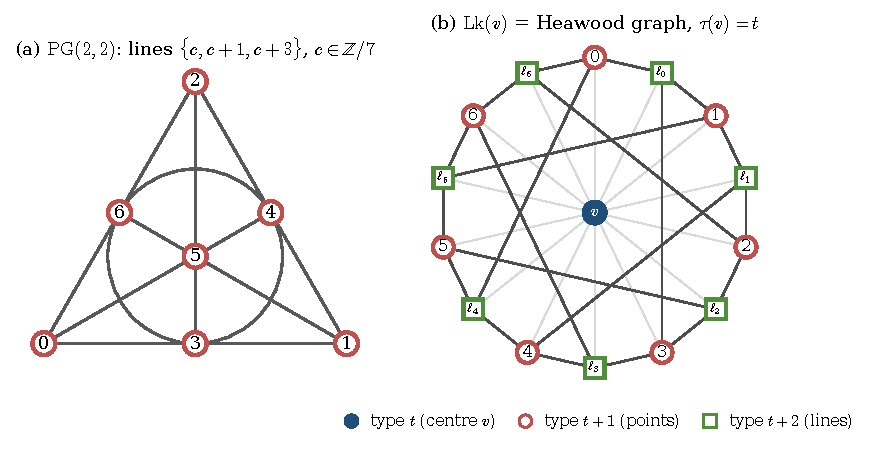
\includegraphics[width=\textwidth]{figures/fig_heawood_fano.pdf}
\caption{The local geometry of the complexes of Vol.~I--II for $q=2$. (a) The Fano plane
$\PG(2,2)$, labelled as in the triangle presentation: its seven lines are the translates
$\{c,c+1,c+3\}$, $c\in\Z/7$, of the Singer difference set $\{0,1,3\}$. (b) The link of a vertex $v$ of
type $t$, which by (L) is the incidence graph of (a), the Heawood graph: its $7$ vertices of type
$t+1$ are the points, its $7$ vertices of type $t+2$ are the lines $\ell_c=\{c,c+1,c+3\}$, and its $21$
edges are the flags, i.e.\ the chambers through $v$ (faint spokes). The three colours are the three
classes of the $\Z/3$ type grading used in Proposition~\ref{V3P1:prop:grading}. Drawn by
\texttt{code/make\_figures.py}.}
\label{V3P1:fig:heawood}
\end{figure}

\begin{lemma}[Counts from the links]\label{V3P1:lem:counts}
Assume \textup{(L)}. Then:
\begin{enumerate}
\item[(a)] $|E|=n(q^{2}+q+1)$, each edge lies in exactly $q+1$ triangles, and
$|F|=\tfrac13\,n(q^{2}+q+1)(q+1)$;
\item[(b)] $\Tr(A_1A_2)=|E|$;
\item[(c)] $\Tr A_1^{3}=3|F|+3s$, where $s\ge0$ is the number of $3$-cycles $x\to y\to z\to
x$ of type-increasing edges whose vertex set is \emph{not} a triangle. So
$\Tr A_1^{3}\ge3|F|$, with equality if and only if the flag condition
\textup{(iv)} of Vol.~I--II, Definition~\ref{M-X:def:a2} holds.
\end{enumerate}
\end{lemma}

\begin{proof}
(a) Count vertex--edge incidences. The edges at $v$ are the vertices of $\mathrm{Lk}(v)$, and
there are $2(q^{2}+q+1)$ of them by Lemma~\ref{V3P1:lem:pg}, so $2|E|=2n(q^{2}+q+1)$. The
triangles through an edge $\{v,w\}$ are the edges of $\mathrm{Lk}(v)$ at $w$, and there are
$q+1$ of them. The triangles at $v$ are the edges of $\mathrm{Lk}(v)$, i.e.\ the flags of
$\PG(2,q)$, so counting vertex--triangle incidences gives
$3|F|=n(q^{2}+q+1)(q+1)$.

(b) Each edge $\{x,y\}$ joins vertices of different types, and exactly one of its two
orientations is type-increasing: if $\tau(y)=\tau(x)+1$ it is $x\to y$, and if
$\tau(y)=\tau(x)+2$ then $\tau(x)=\tau(y)+1$ and it is $y\to x$. Hence $A_1$ has exactly
$|E|$ entries equal to $1$, and $\Tr(A_1A_1^{t})=\sum_{x,y}A_1(x,y)^{2}=|E|$.

(c) $\Tr A_1^{3}$ counts closed walks $x\to y\to z\to x$ of type-increasing edges. Such a walk
visits the three types, so $x,y,z$ are distinct. A triangle $\{a,b,c\}$ with
$\tau=(t,t+1,t+2)$ carries exactly one such cycle, $a\to b\to c\to a$ (the reverse is
type-decreasing), and that cycle contributes three closed walks, one for each starting
point. The remaining closed walks come in cyclic classes of three, one class for each
non-triangle $3$-cycle.
\end{proof}

For $q=2$: $|E|=|F|=7n$, and each vertex sees $14$ edges and $21$ triangles, which are the
$14$ vertices and $21$ edges of the Heawood graph (Figure~\ref{V3P1:fig:heawood}).

\section{The \texorpdfstring{$\Z/3$}{Z/3} grading and the cubic trace identity}\label{V3P1:sec:trace}

\paragraph{The rank-one obstruction.} For a $(q+1)$-regular graph, the companion
$C=\begin{psmallmatrix}T_p&-qI\\ I&0\end{psmallmatrix}$ of the Ihara pencil $1-uT_p+qu^{2}$
satisfies $\Tr C=0$ and
\[
\Tr C^{2}=\Tr T_p^{2}-2qn=n(q+1)-2qn=-n(q-1)<0
\]
[Vol.~I--II, Ch.~\ref{M-chap:II}, Lem.~\ref{M-II:lem:tracecomp}]. The positive term $\Tr T_p^{2}=2|E|$
counts closed walks that return by reversing an edge, and it is beaten by the $-qI$ block,
which is hit twice. By [Vol.~I--II, Ch.~\ref{M-chap:II}, Thm.~\ref{M-II:thm:traceany}] no non-negative
matrix of any size carries this spectrum.

In rank two the companion of the cubic pencil
$P(u)=I-uA_1+qu^{2}A_2-q^{3}u^{3}I$ is
\begin{equation}\label{V3P1:eq:C}
\Cthree=\begin{pmatrix}A_1&-qA_2&q^{3}I\\ I&0&0\\ 0&I&0\end{pmatrix}\in M_{3n}(\Z).
\end{equation}

\begin{proposition}[Grading conjugation]\label{V3P1:prop:grading}
Let $\omega=e^{2\pi i/3}$, $D_1=\operatorname{diag}(\omega^{-\tau(v)})_{v\in V}$ and
$D=\operatorname{diag}(D_1,\ \omega D_1,\ \omega^{2}D_1)$. Then
\[
D_1A_1D_1^{-1}=\omega A_1,\qquad D_1A_2D_1^{-1}=\omega^{2}A_2,\qquad D\,\Cthree D^{-1}=\omega\,\Cthree .
\]
Consequently $\Tr(\Cthree)^{k}=0$ for every $k$ with $3\nmid k$, the spectrum of $\Cthree$
\textup{(}with multiplicities\textup{)} is invariant under multiplication by $\omega$, and
$\det(I-u\Cthree)\in\Z[u^{3}]$.
\end{proposition}

\begin{proof}
$(D_1A_1D_1^{-1})_{xy}=\omega^{\tau(y)-\tau(x)}A_1(x,y)=\omega A_1(x,y)$, because $A_1(x,y)\neq0$
forces $\tau(y)=\tau(x)+1$. Transposing gives $\omega^{-1}=\omega^{2}$ for $A_2$. Write
$D=\operatorname{diag}(d_1D_1,d_2D_1,d_3D_1)$ with $(d_1,d_2,d_3)=(1,\omega,\omega^{2})$.
Block $(i,j)$ of $D\Cthree D^{-1}$ is $d_id_j^{-1}D_1\Cthree_{ij}D_1^{-1}$:
\[
(1,1)\colon\ \omega A_1;\quad
(1,2)\colon\ \omega^{-1}\cdot\omega^{2}(-qA_2)=\omega(-qA_2);\quad
(1,3)\colon\ \omega^{-2}q^{3}I=\omega q^{3}I;\quad
(2,1),(3,2)\colon\ \omega I .
\]
So $D\Cthree D^{-1}=\omega\Cthree$, and therefore $\Tr(\Cthree)^{k}=\omega^{k}\Tr(\Cthree)^{k}$,
which vanishes when $\omega^{k}\neq1$. Similarity of $\Cthree$ and $\omega\Cthree$ gives the
invariance of the spectrum. Then $\det(I-u\Cthree)=\det(I-\omega u\Cthree)$, so only powers
of $u^{3}$ occur.
\end{proof}

\begin{remark}[Walk form of the grading]\label{V3P1:rem:walks}
Every entry of $(\Cthree)^{k}$ is a signed, $q$-weighted sum over words in $A_1$ (one type
step up), $A_2$ (one type step down, i.e.\ two steps up modulo~$3$) and the identity blocks,
which shift the block index but not the vertex. A closed contribution to the trace must
return to its starting vertex, and hence to its starting type. With the block bookkeeping,
the net type change of a word of length $k$ is $\equiv k\pmod 3$. This is the combinatorial
content of $D\Cthree D^{-1}=\omega\Cthree$.
\end{remark}

\begin{theorem}[Cubic trace identity]\label{V3P1:thm:trace}
For every $\Atwo$ complex of order $q$, with or without the flag condition,
\begin{equation}\label{V3P1:eq:trace-general}
\Tr(\Cthree)^{3}=\Tr A_1^{3}-3q\,\Tr(A_1A_2)+3nq^{3}=\Tr A_1^{3}-3q|E|+3nq^{3}.
\end{equation}
Under \textup{(L)} this equals $n(q-1)^{2}(q+1)+3s$, with $s$ as in
Lemma~\ref{V3P1:lem:counts}(c). Under the flag condition,
\begin{equation}\label{V3P1:eq:trace-flag}
\Tr(\Cthree)^{3}=3|F|-3q|E|+3nq^{3}=n(q-1)^{2}(q+1)\ \ge 0,
\end{equation}
with equality if and only if $q=1$.
\end{theorem}

\begin{proof}
Write $\Cthree$ by columns: $\mathrm{col}_1=(A_1,I,0)^{t}$,
$\mathrm{col}_2=(-qA_2,0,I)^{t}$, $\mathrm{col}_3=(q^{3}I,0,0)^{t}$. The rows of $\Cthree$ are
$r_1=(A_1,-qA_2,q^{3}I)$, $r_2=(I,0,0)$ and $r_3=(0,I,0)$. Hence the rows of $(\Cthree)^{2}$
are
\[
r_1\Cthree=\bigl(A_1^{2}-qA_2,\ -qA_1A_2+q^{3}I,\ q^{3}A_1\bigr),\qquad
r_2\Cthree=r_1,\qquad r_3\Cthree=r_2 .
\]
The diagonal blocks of $(\Cthree)^{3}=(\Cthree)^{2}\Cthree$ are
\begin{align*}
\bigl((\Cthree)^{3}\bigr)_{11}&=(A_1^{2}-qA_2)A_1+(-qA_1A_2+q^{3}I)\cdot I+q^{3}A_1\cdot 0\\
&=A_1^{3}-qA_2A_1-qA_1A_2+q^{3}I,\\
\bigl((\Cthree)^{3}\bigr)_{22}&=r_1\cdot\mathrm{col}_2=A_1(-qA_2)+(-qA_2)\cdot0+q^{3}I\cdot I=-qA_1A_2+q^{3}I,\\
\bigl((\Cthree)^{3}\bigr)_{33}&=r_2\cdot\mathrm{col}_3=q^{3}I .
\end{align*}
Summing traces and using $\Tr(A_2A_1)=\Tr(A_1A_2)$ gives \eqref{V3P1:eq:trace-general}.
Each term has a walk meaning. $\Tr A_1^{3}$ counts closed type-increasing $3$-walks.
$\Tr(A_1A_2)=|E|$ counts the backtracking $2$-walks $x\to y\leftarrow x$; it enters three
times, once for each of the three cyclic positions at which the backtrack can sit inside a
$3$-step return, each with weight $-q$. The term $q^{3}$ is the pure constant term, entering
once per block. Under (L), Lemma~\ref{V3P1:lem:counts} gives $\Tr A_1^{3}=3|F|+3s$, and
\begin{align*}
3|F|-3q|E|+3nq^{3}
&=n\bigl[(q^{2}+q+1)(q+1)-3q(q^{2}+q+1)+3q^{3}\bigr]\\
&=n\bigl[(q^{3}+2q^{2}+2q+1)-(3q^{3}+3q^{2}+3q)+3q^{3}\bigr]\\
&=n\,(q^{3}-q^{2}-q+1)=n(q-1)^{2}(q+1).
\end{align*}
Under the flag condition $s=0$. The factor $(q-1)^{2}(q+1)$ vanishes only at $q=1$.
\end{proof}

\begin{remark}[Parity versus $\Z/3$]\label{V3P1:rem:parity}
In rank one a closed walk can return in two steps, so the negative block $-qI$ is felt
already at $k=2$, and it is felt twice. In rank two the grading makes $\Tr(\Cthree)^{k}$
blind to everything for $k=1,2$. At $k=3$ the chamber term $3|F|=n(q^{2}+q+1)(q+1)$, the flag
count of $\PG(2,q)$ times $n$, dominates the backtracking loss $3q|E|-3nq^{3}$. The
difference is exactly $n(q-1)^{2}(q+1)$. This is the proof behind
[Vol.~I--II, Ch.~\ref{M-chap:X}, Thm.~\ref{M-X:thm:notrace}], written out in full, and its consequence for
realizability is recorded in [Vol.~I--II, Ch.~\ref{M-chap:X}, Thm.~\ref{M-X:thm:realizable}].
\end{remark}

% Volume III, Chapter 1 -- addendum: the first nonzero trace of the PGL_{d+1} companion on
% A~_d complexes (open problem (a) of Remark V3P1:rem:scope).  Verified by code/v3p1_ad_trace.py.
\section{The first nonzero trace in every rank}\label{V3P1:sec:tracead}

This section settles open problem (a) of Remark~\ref{V3P1:rem:scope}: the value of the first
nonzero trace $\Tr(C^{(d+1)})^{d+1}$ on $\Atilde d$ complexes. The answer is
$n\prod_{i=1}^{d}(1-q^{i})$ under the $\Atilde d$ flag condition, which contains the rank-one value
$-n(q-1)$ and Theorem~\ref{V3P1:thm:trace} as the cases $d=1,2$.

\paragraph{Setting.} An $\Atilde d$ complex $Y$ has a type map $\tau\colon V\to\Z/(d+1)$, and for
$1\le j\le d$ we let $A_j$ be the $0/1$ matrix with $A_j(x,y)=1$ iff $\{x,y\}$ is an edge and
$\tau(y)=\tau(x)+j$; put $A_{d+1}=I$. The local hypothesis replacing (L) is
\begin{itemize}
\item[(L$_d$)] the link of every vertex $v$ is isomorphic to the flag complex of $\PG(d,q)$, the
neighbours of type $\tau(v)+i$ going to the subspaces of codimension $i$ in $\F_q^{d+1}$
($1\le i\le d$), adjacency in the link being containment. By the duality $U\mapsto U^{\perp}$ one
may equally send them to the subspaces of dimension $i$; for $d=2$ that is \textup{(L)}.
\end{itemize}
A \emph{closed walk of increments} $\mathbf j=(j_1,\dots,j_r)$, $j_i\ge1$, is a sequence
$x_0\to x_1\to\dots\to x_r=x_0$ with $A_{j_i}(x_{i-1},x_i)=1$ (the identity step for $j_i=d+1$). The
\emph{flag condition} of rank $d$ is
\begin{itemize}
\item[(F$_d$)] every closed walk whose increments sum to $d+1$ has all its vertices in one simplex.
\end{itemize}
For $d=2$ the only increments with sum $3$ are $(1,1,1)$, $(1,2)$, $(2,1)$ and $(3)$, and (F$_2$) is the
flag condition of Lemma~\ref{V3P1:lem:counts}(c). The companion is
\[
C^{(d+1)}=\begin{pmatrix}
R_1&R_2&\cdots&R_d&R_{d+1}\\ I&0&\cdots&0&0\\ &\ddots&&&\vdots\\ 0&\cdots&&I&0\end{pmatrix},
\qquad R_j=(-1)^{j-1}q^{\binom j2}A_j ,
\]
which is \eqref{V3P1:eq:C} for $d=2$. When the $A_j$ commute, $\det(xI-C^{(d+1)})=\sum_{j=0}^{d+1}(-1)^{j}
q^{\binom j2}A_jx^{d+1-j}$, the local Hecke polynomial of $\PGL_{d+1}$; the companion of
[Vol.~I--II, Ch.~\ref{M-chap:XX}, Thm.~\ref{M-XX:thm:hecke}] has the same excursion weights $R_j$
(see the proof of Lemma~\ref{V3P1:lem:excursion}), hence the same traces of all powers. With
$D_1=\operatorname{diag}(\zeta^{-\tau})$, $\zeta=e^{2\pi i/(d+1)}$, the proof of
Proposition~\ref{V3P1:prop:grading} gives $DC^{(d+1)}D^{-1}=\zeta C^{(d+1)}$ verbatim, so
$\Tr(C^{(d+1)})^{k}=0$ for $(d+1)\nmid k$.

\begin{lemma}[Excursion expansion]\label{V3P1:lem:excursion}
For every $k\ge1$, with no commutativity assumption,
\[
\Tr\bigl(C^{(d+1)}\bigr)^{k}=\sum_{\mathbf j}\,j_1\,(-1)^{k-r}\,q^{\sum_i\binom{j_i}2}\,
\Tr\bigl(A_{j_1}A_{j_2}\cdots A_{j_r}\bigr),
\]
the sum over the compositions $\mathbf j=(j_1,\dots,j_r)$ of $k$ with all parts $\le d+1$.
\end{lemma}

\begin{proof}
$\bigl((C^{(d+1)})^{k}\bigr)_{bb}$ is a sum over closed walks of length $k$ in the graph on the block
indices $1,\dots,d+1$ whose arcs are $1\to j$ (weight $R_j$) and $i+1\to i$ (weight $I$). From block
$1$, the arc $1\to j$ must be followed by $j\to j-1\to\dots\to1$, so every return to block $1$ is an
\emph{excursion} of length $j$ and weight $R_j$. A closed walk of length $k$ is therefore a cyclic
sequence of excursions of lengths $j_1,\dots,j_r$ with $\sum j_i=k$, together with the time at which
it starts. Label the excursions so that the walk starts inside the first one; there are $j_1$ such
starting times, and each contributes the trace of a cyclic rotation of $R_{j_1}\cdots R_{j_r}$, which
is $\Tr(R_{j_1}\cdots R_{j_r})$. Finally $\prod_i(-1)^{j_i-1}=(-1)^{k-r}$. For the companion of
[Vol.~I--II, Ch.~\ref{M-chap:XX}], whose row $0$ carries $q^{i}A_{i+1}$ and whose subdiagonal carries
$-q^{i}I$, an excursion of length $j$ has weight
$q^{j-1}A_j\prod_{l=0}^{j-2}(-q^{l})=(-1)^{j-1}q^{\binom j2}A_j=R_j$. Line (W) checks the expansion
as an identity of non-commutative polynomials for $d\le6$, $k\le d+1$.
\end{proof}

\begin{lemma}[Closed walks are flags]\label{V3P1:lem:flagwalks}
Let $\mathbf j$ be a composition of $d+1$ and let $\binom{d+1}{\mathbf j}_q=[d+1]_q!/\prod_i[j_i]_q!$ be
the $q$-multinomial coefficient, $[k]_q=1+q+\dots+q^{k-1}$.
\begin{enumerate}
\item[(i)] Under \textup{(L$_d$)}, $\Tr(A_{j_1}\cdots A_{j_r})=n\binom{d+1}{\mathbf j}_q+s_{\mathbf j}$,
where $s_{\mathbf j}\ge0$ is the number of closed walks of increments $\mathbf j$ whose vertices are not
contained in one simplex. Under \textup{(F$_d$)}, $s_{\mathbf j}=0$.
\item[(ii)] The Bruhat--Tits building of $\PGL_{d+1}$ over a non-archimedean local field with
residue field $\F_q$ satisfies \textup{(L$_d$)} and \textup{(F$_d$)}.
\end{enumerate}
\end{lemma}

\begin{proof}
(i) A closed walk of increments $\mathbf j$ starting at $x_0$ whose vertices lie in a simplex is
determined by $x_1,\dots,x_{r-1}$, which have types $\tau(x_0)+j_1+\dots+j_i$ and form a simplex of
$\mathrm{Lk}(x_0)$, i.e.\ by (L$_d$) a chain $\F_q^{d+1}\supsetneq U_1\supsetneq\dots\supsetneq
U_{r-1}\supsetneq0$ with $\operatorname{codim}(U_i\subset U_{i-1})=j_i$. Conversely every such chain gives
such a walk, the last step $x_{r-1}\to x_0$ having increment $j_r$. The number of chains is the
$q$-multinomial coefficient (choose $U_{r-1}$, then $U_{r-2}\supset U_{r-1}$, and so on), whatever the
order of the parts. The remaining closed walks are counted by $s_{\mathbf j}$.

(ii) The vertices are the homothety classes of lattices $L\subset K^{d+1}$, with uniformizer
$\pi$; $[L]\to[L']$ has increment $j$ iff there are representatives with $L\supset L'\supset\pi L$ and
$\dim L/L'=j$, and the simplices are the chains of such lattices. The link of $[L]$ is the flag complex
of $L/\pi L\cong\F_q^{d+1}$. Given a closed walk $x_0\to\dots\to x_r=x_0$ with increments summing to
$d+1$, choose $L_0$ in $x_0$ and inductively the unique representative $L_i$ of $x_i$ with
$L_{i-1}\supset L_i\supset\pi L_{i-1}$. Then $[L_0:L_r]=q^{d+1}$ and $L_r$ is homothetic to $L_0$,
so $L_r=\pi L_0$. Hence $L_0\supset L_1\supset\dots\supset L_{r-1}\supset\pi L_0$ is a chain, and the
vertices of the walk span a simplex.
\end{proof}

\begin{theorem}[First nonzero trace in rank $d$]\label{V3P1:thm:tracead}
Let $Y$ be a finite $\Atilde d$ complex satisfying \textup{(L$_d$)}, with $n$ vertices. Then
$\Tr(C^{(d+1)})^{k}=0$ for $(d+1)\nmid k$, and
\[
\Tr\bigl(C^{(d+1)}\bigr)^{d+1}=n\prod_{i=1}^{d}\bigl(1-q^{i}\bigr)
+\sum_{\mathbf j}j_1(-1)^{d+1-r}q^{\sum_i\binom{j_i}2}s_{\mathbf j}.
\]
Under the flag condition \textup{(F$_d$)},
\[
\Tr\bigl(C^{(d+1)}\bigr)^{d+1}=n\prod_{i=1}^{d}\bigl(1-q^{i}\bigr)=(-1)^{d}\,n\,(q-1)^{d}\,[d]_q!\,.
\]
For $d=1,2,3,4$ this is $-n(q-1)$, $n(q-1)^{2}(q+1)$, $-n(q-1)^{3}(q+1)(q^{2}+q+1)$ and
$n(q-1)^{4}(q+1)^{2}(q^{2}+1)(q^{2}+q+1)$.
\end{theorem}

\begin{proof}
By Lemmas~\ref{V3P1:lem:excursion} and~\ref{V3P1:lem:flagwalks} it remains to show, with $m=d+1$,
\[
T_m:=\sum_{\mathbf j\models m}j_1(-1)^{m-r}q^{\sum\binom{j_i}2}\binom{m}{\mathbf j}_q=\prod_{i=1}^{m-1}(1-q^{i}).
\]
Write $\binom{m}{\mathbf j}_q=[m]_q!\prod_iE_{j_i}$ with $E_j=q^{\binom j2}/[j]_q!$ and work in
$\Z[[q]][[t]]$. Put $F(t)=\sum_{j\ge1}(-1)^{j-1}E_jt^{j}$. Expanding $tF'(t)/(1-F(t))$ by the geometric
series gives $\sum_{\mathbf j}j_1\prod_i(-1)^{j_i-1}E_{j_i}t^{\sum j_i}$, the $j_1$ coming from the
derivative applied to the first factor; hence $T_m=[m]_q!\,[t^{m}]\bigl(-t\tfrac{d}{dt}\log(1-F(t))\bigr)$.
Now $1-F(t)=\sum_{j\ge0}q^{\binom j2}(-t)^{j}/[j]_q!$, and since $[j]_q!=(q;q)_j/(1-q)^{j}$, Euler's
identity $\sum_jq^{\binom j2}z^{j}/(q;q)_j=\prod_{i\ge0}(1+zq^{i})$ with $z=-(1-q)t$ gives
$1-F(t)=\prod_{i\ge0}\bigl(1-(1-q)q^{i}t\bigr)$. Therefore
\[
-t\frac{d}{dt}\log(1-F(t))=\sum_{i\ge0}\frac{(1-q)q^{i}t}{1-(1-q)q^{i}t}
=\sum_{k\ge1}t^{k}\,(1-q)^{k}\sum_{i\ge0}q^{ik}=\sum_{k\ge1}t^{k}\frac{(1-q)^{k}}{1-q^{k}},
\]
and $T_m=[m]_q!\,(1-q)^{m}/(1-q^{m})=\prod_{i=1}^{m}(1-q^{i})/(1-q^{m})=\prod_{i=1}^{m-1}(1-q^{i})$.
Both sides are polynomials in $q$, so the identity in $\Z[[q]]$ is an identity of polynomials. The
last form uses $1-q^{i}=-(q-1)[i]_q$.
\end{proof}

\begin{corollary}\label{V3P1:cor:tracead}
Assume \textup{(L$_d$)} and \textup{(F$_d$)}.
\begin{enumerate}
\item[(i)] As a polynomial in $q$, $\Tr(C^{(d+1)})^{d+1}/n$ vanishes at $q=1$ to order exactly $d$. A
thin complex ($q=1$) satisfying \textup{(F$_d$)} has $\Tr(C^{(d+1)})^{d+1}=0$.
\item[(ii)] For $q\ge2$ the sign of $\Tr(C^{(d+1)})^{d+1}$ is $(-1)^{d}$. For odd $d$ it is negative, so
no non-negative matrix, of any size, has the nonzero spectrum of $C^{(d+1)}$ (with multiplicities):
the obstruction of the rank-one paragraph of Section~\ref{V3P1:sec:trace} recurs in every odd rank,
and disappears in every even rank.
\item[(iii)] On the constants, $A_j$ acts by $\binom{d+1}j_q$ and the local factor is
$\prod_{i=0}^{d}(1-q^{i}u)$; its derivative at $u=1$ is $-\prod_{i=1}^{d}(1-q^{i})$. So the coincidence
of Remark~\ref{V3P1:rem:coincidence} persists in every rank: the first nonzero trace per vertex and the
derivative of the trivial local factor at $u=1$ are the same number up to sign.
\end{enumerate}
\end{corollary}

\begin{proof}
(i) Each factor $1-q^{i}$ has a simple zero at $q=1$. (ii) Each factor is negative for $q\ge2$. The
traces of the powers of a non-negative matrix are non-negative, and padding by zeros does not change
them. (iii) $\sum_j(-1)^{j}q^{\binom j2}\binom{d+1}j_qx^{d+1-j}=\prod_{i=0}^{d}(x-q^{i})$ by the
$q$-binomial theorem, and differentiate.
\end{proof}

\begin{remark}[Numerical record]\label{V3P1:rem:traceadnum}
\texttt{code/v3p1\_ad\_trace.py} (numpy, scipy, sympy; about two minutes) checks: the excursion
expansion as non-commutative words (W); the identity $T_m=\prod_{i<m}(1-q^{i})$ symbolically for
$d\le12$, the order of the zero at $q=1$ and the sign (Q); the chain counts in $\F_q^{d+1}$ by
enumeration of all subspaces for $(d,q)=(2,2),(3,2),(2,3),(3,3),(4,2)$, with per-vertex traces $3$,
$-21$, $16$, $-416$, $315$ (F); the thin $\Atilde d$ tori $(\Z/m)^{d+1}/\Z(1,\dots,1)$ for $d=2,3,4$, which
satisfy \textup{(F$_d$)} for $m\ge d+2$ and give $\Tr(C^{(d+1)})^{d+1}=0$ there, while for $m=d+1$ the
excess walks of increments $(1,\dots,1)$ give $\Tr=(d+1)n$ (T); and $Y_{21}$, where
$651=63+3\cdot196$ (Y). No finite thick $\Atilde3$ complex is constructed; for $d\ge3$ the thick case
rests on Lemma~\ref{V3P1:lem:flagwalks}(ii) and on the per-vertex count (F).
\end{remark}

\begin{remark}[Corrections to the proposed programme]\label{V3P1:rem:traceadcorr}
(1) The proposed $\Tr(C^{(4)})^{4}=n(q-1)^{3}(q+1)(q^{2}+1)$ is false: the value is
$-n(q-1)^{3}(q+1)(q^{2}+q+1)$, e.g.\ $-21n$ instead of $15n$ at $q=2$; the sign is negative and the
last factor is $[3]_q$, not $q^{2}+1$. (2) The proposed general form
$n(q-1)^{d}\prod_j(q^{j+1}-1)/(q-1)$ is false; the correct product is $(-1)^{d}n(q-1)^{d}[d]_q!$. (3) For
$d\ge3$ the trace is not a combination of the cell numbers $|F_k|$ alone: the words $A_{j_1}\cdots
A_{j_r}$ count partial flags of every type, which is why the $q$-multinomials enter. (4) The vertex
block of $L_E$ for $d\ge3$ (Chapter~\ref{chap:V3P4}, Remark~\ref{V3P4:rem:scope}(a)) is a different problem and is not
addressed here.
\end{remark}


\section{Garland rigidity by the local spectral gap}\label{V3P1:sec:garland}

\paragraph{Unitary local systems.} A rank-$N$ unitary local system $\mathcal E$ on a finite
simplicial complex $Y$ is given by a Hermitian space $\mathcal E_v\cong\C^{N}$ at each vertex
and a unitary transport $g_{uv}\colon\mathcal E_v\to\mathcal E_u$ for each oriented edge, with
$g_{vu}=g_{uv}^{-1}$ and $g_{ab}g_{bc}=g_{ac}$ on every triangle (flatness). Equivalently, it
is a representation $\rho\colon\pi_1(Y)\to U(N)$ up to conjugation, and the trivial system
$\mathcal E=\C$ gives ordinary cohomology. Cochains are
\[
C^{0}=\{\varphi(v)\in\mathcal E_v\},\quad
C^{1}=\{f(u,v)\in\mathcal E_u:\ f(v,u)=-g_{vu}f(u,v)\},
\]
and $C^{2}$ consists of alternating functions on oriented triangles with values in the fibre
at the first vertex. The differentials are
\[
(\delta\varphi)(u,v)=g_{uv}\varphi(v)-\varphi(u),\qquad
(\delta f)(a,b,c)=f(a,b)+g_{ab}f(b,c)+g_{ac}f(c,a).
\]
Flatness gives $\delta\delta=0$:
$(\delta\delta\varphi)(a,b,c)=g_{ab}g_{bc}\varphi(c)-g_{ac}\varphi(c)=0$.

\paragraph{Weights.} Let $m(e)$ be the number of triangles containing the edge $e$, and
$m(v)=\sum_{w\sim v}m(vw)$. We put
\[
\langle\varphi,\psi\rangle=\sum_vm(v)\langle\varphi(v),\psi(v)\rangle,\qquad
\langle f,h\rangle=\tfrac12\sum_{(u,v)}m(uv)\langle f(u,v),h(u,v)\rangle,
\]
where the second sum is over oriented edges. It is well defined because transport is unitary.
Under (L), $m(e)=q+1$ and $m(v)=2(q+1)(q^{2}+q+1)$ are constant, so these are scalar multiples
of the standard inner products, and the harmonic forms below are the standard ones.

\begin{lemma}[Adjoint and Hodge]\label{V3P1:lem:adjoint}
$(\delta^{*}f)(u)=-\frac1{m(u)}\sum_{v\sim u}m(uv)f(u,v)$, and
$H^{1}(Y;\mathcal E)\cong\ker\delta\cap\ker\delta^{*}\subseteq C^{1}$.
\end{lemma}

\begin{proof}
Start from $\langle\delta\varphi,f\rangle=\tfrac12\sum_{(u,v)}m(uv)\bigl(\langle g_{uv}\varphi(v),
f(u,v)\rangle-\langle\varphi(u),f(u,v)\rangle\bigr)$. By unitarity and antisymmetry,
$\langle g_{uv}\varphi(v),f(u,v)\rangle=\langle\varphi(v),g_{vu}f(u,v)\rangle
=-\langle\varphi(v),f(v,u)\rangle$. Relabelling $(u,v)\leftrightarrow(v,u)$ turns the first
sum into the second, so $\langle\delta\varphi,f\rangle=-\sum_{(u,v)}m(uv)\langle\varphi(u),
f(u,v)\rangle$, which is the stated adjoint. Since $C^{1}=\operatorname{im}\delta\oplus
(\operatorname{im}\delta)^{\perp}$ and $(\operatorname{im}\delta)^{\perp}=\ker\delta^{*}$,
every class in $\ker\delta/\operatorname{im}\delta$ has a unique representative in
$\ker\delta\cap\ker\delta^{*}$.
\end{proof}

\begin{lemma}[Spectrum of the link]\label{V3P1:lem:gap}
The adjacency eigenvalues of $\mathcal I(q)$ are $\pm(q+1)$, each simple, and $\pm\sqrt q$,
each with multiplicity $q^{2}+q$. The normalized Laplacian $I-\frac1{q+1}\mathrm{Adj}$
therefore has smallest positive eigenvalue
\[
\lambda(q)=1-\frac{\sqrt q}{q+1},\qquad\text{and}\qquad 2\lambda(q)-1=\frac{(\sqrt q-1)^{2}}{q+1}.
\]
So $\lambda(q)>\tfrac12$ for every $q\ge2$ and $\lambda(1)=\tfrac12$. For the Heawood graph,
$\lambda(2)=1-\sqrt2/3=0.528595\ldots$
\end{lemma}

\begin{proof}
Let $N$ be the point--line incidence matrix. By Lemma~\ref{V3P1:lem:pg},
$NN^{t}=(q+1)I+(J-I)=qI+J$, since a point lies on $q+1$ lines and two points share one line.
Its eigenvalues are $q+(q^{2}+q+1)=(q+1)^{2}$ on $\mathbf 1$ and $q$ on $\mathbf 1^{\perp}$.
The adjacency $\begin{psmallmatrix}0&N\\N^{t}&0\end{psmallmatrix}$ has eigenvalues
$\pm\sqrt{\,\cdot\,}$ of these, and the graph is $(q+1)$-regular. The simplicity of $q+1$
shows that $\mathcal I(q)$ is connected.
\end{proof}

For a $\mathcal E_v$-valued function $\phi$ on $\mathrm{Lk}(v)$ put
$\|\phi\|^{2}_{v}=\sum_{w}m(vw)|\phi(w)|^{2}$ and $\|d\phi\|^{2}_{v}=\sum_{\{w,x\}}|\phi(x)-\phi(w)|^{2}$,
the second sum running over link edges, i.e.\ over triangles $\{v,w,x\}$. The degree of $w$
in $\mathrm{Lk}(v)$ is $m(vw)$. So if $\sum_wm(vw)\phi(w)=0$, then
$\|d\phi\|_v^{2}\ge\lambda(q)\|\phi\|_v^{2}$, applying Lemma~\ref{V3P1:lem:gap} componentwise
in an orthonormal basis of $\mathcal E_v$.

\begin{theorem}[Garland vanishing, local form]\label{V3P1:thm:garland}
Let $Y$ be a finite two-dimensional simplicial complex satisfying \textup{(L)} with $q\ge2$.
No building, free action or flag condition is assumed. Then $H^{1}(Y;\mathcal E)=0$ for every
unitary local system $\mathcal E$ on $Y$. In particular:
\begin{enumerate}
\item[(i)] $b_1(Y;\R)=b_1(Y;\C)=0$, and $H_1(Y;\Z)$ is a finite abelian group;
\item[(ii)] $\coker_\Z\Delta_1=\Jac_1(Y)$, i.e.\ the edge critical group is the whole cokernel;
the group $K(Y)=\ker\partial_1/\operatorname{im}(\partial_2\partial_2^{t})$ is finite and
surjects onto $H_1(Y;\Z)$; and $b_2=\chi(Y)-1$;
\item[(iii)] every finite connected cover $Y'\to Y$ satisfies \textup{(L)}, hence (i)--(ii).
\end{enumerate}
\end{theorem}

\begin{proof}
Let $f\in\ker\delta\cap\ker\delta^{*}$ (Lemma~\ref{V3P1:lem:adjoint}). For each vertex $v$
define the localization $f_v(w):=f(v,w)\in\mathcal E_v$ for $w\in\mathrm{Lk}(v)$. All of its
values lie in the \emph{single} fibre $\mathcal E_v$, so no trivialization is needed. We prove
three identities.

\emph{(a) Mass.} $\sum_v\|f_v\|_v^{2}=\sum_v\sum_{w\sim v}m(vw)|f(v,w)|^{2}
=\sum_{(v,w)}m(vw)|f(v,w)|^{2}=2\|f\|^{2}$.

\emph{(b) Energy.} Fix a triangle $\{a,b,c\}$; it is the link edge $\{b,c\}$ of
$\mathrm{Lk}(a)$. Since $\delta f=0$ and $g_{ac}f(c,a)=-f(a,c)$,
\[
f_a(c)-f_a(b)=f(a,c)-f(a,b)=g_{ab}f(b,c),\qquad\text{so}\qquad |f_a(c)-f_a(b)|=|f(b,c)|.
\]
Summing over the three vertices of every triangle,
$\sum_v\|df_v\|_v^{2}=\sum_{\{a,b,c\}\in F}\bigl(|f(b,c)|^{2}+|f(c,a)|^{2}+|f(a,b)|^{2}\bigr)
=\sum_{e}m(e)|f(e)|^{2}=\|f\|^{2}$.

\emph{(c) Balance.} $\sum_{w}m(vw)f_v(w)=-m(v)(\delta^{*}f)(v)=0$.

By (c) and Lemma~\ref{V3P1:lem:gap}, $\|df_v\|_v^{2}\ge\lambda(q)\|f_v\|_v^{2}$ for every $v$.
Summing and using (a) and (b),
\[
\|f\|^{2}=\sum_v\|df_v\|_v^{2}\ \ge\ \lambda(q)\sum_v\|f_v\|_v^{2}=2\lambda(q)\|f\|^{2},
\qquad\text{i.e.}\qquad \frac{(\sqrt q-1)^{2}}{q+1}\,\|f\|^{2}\le0 .
\]
Hence $f=0$ for $q\ge2$. For (i), take $\mathcal E$ trivial: $H^{1}(Y;\C)=0$, so $b_1=0$, and
$H_1(Y;\Z)$ is finitely generated of rank $0$. For (ii), $\coker\Delta_1\cong\Z^{b_1}\oplus
\Jac_1(Y)$ by Vol.~I--II, Proposition~\ref{M-X:prop:hodge}. $K(Y)$ has rank $\rank\ker\partial_1-
\rank\partial_2=b_1=0$, and it surjects onto $\ker\partial_1/\operatorname{im}\partial_2=
H_1(Y;\Z)$ because $\operatorname{im}(\partial_2\partial_2^{t})\subseteq\operatorname{im}
\partial_2$. Finally $\chi=b_0-b_1+b_2$. For (iii), links are local, and a covering map is a
simplicial isomorphism on stars.
\end{proof}

\begin{remark}[Sharpness and provenance]\label{V3P1:rem:sharp}
At $q=1$ the link is the hexagon, $2\lambda(1)-1=0$, and the inequality is empty. The thin
tori of Vol.~I--II, Construction~\ref{M-X:con:thin} indeed have $b_1=2$, so the threshold
$\lambda>\tfrac12$ is exactly where rank two separates from flat. The argument is Garland's
local-to-global method \cite{Ga}, in the form isolated by Ballmann--\'Swi\k{a}tkowski
\cite{BSw} and \.Zuk \cite{Zuk96}. We have written it for unitary local systems because this
costs nothing and gives Proposition~\ref{V3P1:prop:rigid}. It sharpens
[Vol.~I--II, Ch.~\ref{M-chap:XII}, Thm.~\ref{M-XII:thm:noabelian}] in two respects: no group action is used,
and the flag condition is not needed. The latter matters because four of the five complexes
of [Vol.~I--II, Ch.~\ref{M-chap:X}] violate it.
\end{remark}

\begin{remark}[Correction to {[Vol.~I--II, Ch.~\ref{M-chap:Phys1}, Rem.~\ref{M-Phys1:rem:global}]}]\label{V3P1:rem:physcorr}
That remark asserts that ``no local inspection of a rank-two hyperbolic lattice reveals the
obstruction''. Theorem~\ref{V3P1:thm:garland} shows the opposite for $b_1$. The vanishing of
$b_1$ is certified by the vertex links alone, through the single number
$\lambda(2)=1-\sqrt2/3>\tfrac12$ of the Heawood graph. What is genuinely global is the finite
group $H_1(Y;\Z)$ itself, e.g.\ $(\Z/2)^{6}$ versus $(\Z/2)^{3}\oplus(\Z/4)^{2}$ for two
complexes with identical links, and property (T) of $\pi_1(Y)$.
\end{remark}

\begin{remark}[$\Atilde d$, $d\ge3$]\label{V3P1:rem:Ad}
Since $H^{1}$ depends only on the $2$-skeleton, the proof above applies to an $\Atilde d$
complex as soon as the $1$-skeleton of each vertex link (the spherical building of $\PG(d,q)$,
weighted by triangle counts) has normalized spectral gap $>\tfrac12$. We have not computed that
gap for $d\ge3$, and we do not claim it. For thick $\Atilde d$ buildings with $d\ge3$,
$b_1=0$ of finite free quotients follows instead from Tits' theorem that such buildings are
Bruhat--Tits and from Kazhdan's property (T) for simple groups of rank $\ge2$ over local
fields. These are quoted, not proved here, and nothing below uses them.
\end{remark}

\section{What rigidity removes: Brillouin zones, abelian towers, and the non-commutative turn}\label{V3P1:sec:turn}

\begin{proposition}[No continuous character families]\label{V3P1:prop:rigid}
Let $Y$ satisfy \textup{(L)} with $q\ge2$.
\begin{enumerate}
\item[(i)] $\Hom(\pi_1(Y),U(1))=\Hom(H_1(Y;\Z),U(1))$ is a finite group, isomorphic to
$H_1(Y;\Z)$. For every $\chi$ in it, $H^{1}(Y;\C_\chi)=0$.
\item[(ii)] For every unitary $\rho\colon\pi_1(Y)\to U(N)$, $H^{1}(\pi_1(Y);\mathfrak{gl}_N(\C)_{\mathrm{Ad}\rho})=0$.
Hence, by Weil's criterion, every first-order deformation of $\rho$ in
$\Hom(\pi_1(Y),\GL_N(\C))$ is tangent to its conjugation orbit: unitary representations are
infinitesimally rigid, and the unitary character variety has no positive-dimensional
component through any point.
\end{enumerate}
\end{proposition}

\begin{proof}
(i) $U(1)$ is abelian, $H_1(Y;\Z)$ is finite (Theorem~\ref{V3P1:thm:garland}), and a finite
abelian group is isomorphic to its Pontryagin dual. Then apply Theorem~\ref{V3P1:thm:garland}
to the rank-one system $\C_\chi$. (ii) $\mathrm{Ad}\rho$ preserves the Hilbert--Schmidt
product $\operatorname{tr}(X^{*}Y)$, so it defines a unitary local system of rank $N^{2}$. In
degree one, $H^{1}(\pi_1(Y);V)=H^{1}(Y;\mathcal V)$ for any connected CW complex. Apply
Theorem~\ref{V3P1:thm:garland}. Weil's criterion \cite{Wei64} identifies the Zariski tangent
space of the representation variety at $\rho$ with the cocycles $Z^{1}(\pi_1(Y);
\mathfrak{gl}_N)$, and the tangent space to the orbit with the coboundaries.
\end{proof}

\begin{remark}[Brillouin zones]\label{V3P1:rem:bz}
Bloch--Floquet theory for a $\Z^{d}$-periodic operator decomposes it over the torus
$\widehat{\Z^{d}}=\Hom(\Z^{d},U(1))$, the Brillouin zone. For a periodic operator on the
maximal abelian cover of $Y$ (Hecke operators, the Hodge Laplacians, or any tight-binding
Hamiltonian), the same decomposition runs over $\Hom(H_1(Y;\Z),U(1))$. By
Proposition~\ref{V3P1:prop:rigid}(i) this is a \emph{finite} set of $|H_1(Y;\Z)|$ points, and
the Bloch decomposition is a finite direct sum of twisted operators: $64$ of them for $Y_{21}$
and $128$ for $Y_{42}$ (Section~\ref{V3P1:sec:examples}). There is no continuous momentum, and
therefore no band, group velocity or effective mass. Part~(ii) says more: no continuous
family of \emph{non-abelian} unitary twists exists either, even infinitesimally. This is the
precise content of ``the Brillouin zone is erased'', and it strengthens
[Vol.~I--II, Ch.~\ref{M-chap:Phys1}, Thm.~\ref{M-Phys1:thm:nogo}]. That theorem obtained (iv) from property
(T) of the group; here the rigidity is derived from the links.
\end{remark}

\begin{proposition}[Galois towers over $Y$]\label{V3P1:prop:fab}
Let $Y$ satisfy \textup{(L)} with $q\ge2$, and let $G$ be the profinite Galois group of a tower
of finite connected Galois covers $(Y_U)_U$ of $Y$, indexed by the open normal subgroups
$U\le G$.
\begin{enumerate}
\item[(i)] Every open subgroup $U\le G$ has finite abelianization
$U^{\mathrm{ab}}=U/\overline{[U,U]}$.
\item[(ii)] In particular no open subgroup of $G$ surjects onto $\Z_\ell$. There are no
$\Z_\ell$-towers, and no $\Z_\ell^{r}$-towers for any $r\ge1$, over any finite cover of $Y$.
The commutative Iwasawa theory of {\rm[Vol.~I--II, Chs.~\ref{M-chap:IV}, \ref{M-chap:IX}]} has no rank-two
sector.
\item[(iii)] If $G$ is an infinite $\ell$-adic analytic group with Lie algebra $\mathfrak g$,
then $[\mathfrak g,\mathfrak g]=\mathfrak g$, and $\mathfrak g$ has a nonzero semisimple Levi
factor. So $\dim G\ge3$, and the Iwasawa algebra $\Z_\ell[[G]]$ is non-commutative.
\end{enumerate}
\end{proposition}

\begin{proof}
(i) The cover $Y_U$ is a finite connected cover of $Y$, so $H_1(Y_U;\Z)$ is finite by
Theorem~\ref{V3P1:thm:garland}(iii). The tower gives a homomorphism
$\pi_1(Y_U)\to U$ with dense image. Hence the image of $H_1(Y_U;\Z)=\pi_1(Y_U)^{\mathrm{ab}}$
in $U^{\mathrm{ab}}$ is dense, and being finite, it is closed; so $U^{\mathrm{ab}}$ is
finite. (ii) A continuous surjection $U\to\Z_\ell$ would factor through $U^{\mathrm{ab}}$.
(iii) Uses Lazard's theory \cite{Laz65,DDMS}, quoted. Suppose $[\mathfrak g,\mathfrak g]\neq
\mathfrak g$, and choose a nonzero $\Q_\ell$-linear $\mu\colon\mathfrak g\to\Q_\ell$ vanishing
on $[\mathfrak g,\mathfrak g]$. On a uniform open subgroup $U$, $\log\colon U\to\mathfrak g$
converts the group law into the Baker--Campbell--Hausdorff series. All terms of that series
beyond $\log x+\log y$ are iterated brackets, and $\mu$ kills them, so $\mu\circ\log$ is a
continuous homomorphism $U\to\Q_\ell$. It is nonzero, since $\log U$ spans $\mathfrak g$, and
its image is a nonzero compact subgroup of $\Q_\ell$, hence infinite. This contradicts (i).
A perfect Lie algebra is not solvable unless it is $0$, so by Levi's theorem it has a nonzero
semisimple part, of dimension $\ge3$.
\end{proof}

\begin{remark}[The non-commutative turn]\label{V3P1:rem:turn}
The proposed programme asks why, without abelian towers, one ``must turn to non-linear dynamical
modes and non-commutative group algebras''. The precise statements are the following.
(1) Abelian harmonic analysis over a continuous dual group, which underlies Brillouin zones,
Fourier analysis on $\Z_\ell$-towers and the Iwasawa module $\XX$ over $\Z_\ell[[T]]$, has
nothing to act on. By Propositions~\ref{V3P1:prop:rigid} and~\ref{V3P1:prop:fab}, every
infinite Galois structure over $Y$ is non-abelian of dimension $\ge3$, and its natural
coefficient ring is a non-commutative Iwasawa algebra $\Z_\ell[[G]]$ in the sense of
\cite{CFKSV}. On finite levels, the decomposition along irreducible representations of the
deck group is the character mechanism of [Vol.~I--II, Ch.~\ref{M-chap:XII}, Thm.~\ref{M-XII:thm:norm}].
Whether $\pi_1(Y)$ admits such an infinite $\ell$-adic analytic tower depends on its
linearity, which we do not decide for the complexes of [Vol.~I--II, Ch.~\ref{M-chap:X}].
(2) The infinite structures that survive without any group are \emph{dynamical}. They are the
symbolic dynamics of $\Cthree$ and of its three-step reduction $\Lambda_Q$
(Vol.~I--II, Definition~\ref{M-X:def:reduced}), the geodesic and chamber digraph towers $E_k$, $F_k$ of
[Vol.~I--II, Ch.~\ref{M-chap:XII}], and the Kirchberg algebras $\cO(Y,\DeltaH)$ of
[Vol.~I--II, Ch.~\ref{M-chap:X}, Thm.~\ref{M-X:thm:shadow}]. These are towers of shifts, not of covers. The
phrase ``non-linear dynamical modes'' is not given a mathematical meaning here, and we
replace it by (1) and (2).
\end{remark}

\section{The Hecke--Laplacian and the spectrum of the cubic pencil}\label{V3P1:sec:pencil}

Recall $P(u)=I-uA_1+qu^{2}A_2-q^{3}u^{3}I$ and $\DeltaH=-P(1)=(q^{3}-1)I+A_1-qA_2$
(Vol.~I--II, Definition~\ref{M-X:def:pencil}). Since $A_1$ is normal ($A_1A_1^{t}=A_1^{t}A_1$), $A_1$ and
$A_2=A_1^{*}$ are simultaneously unitarily diagonalizable. The joint eigenpairs are
$(a_j,\bar a_j)$, $j=1,\dots,n$, and $P_j(u)=1-a_ju+q\bar a_ju^{2}-q^{3}u^{3}$. Put
$\kappa:=q^{2}+q+1$.

\begin{theorem}[Pencil determinant]\label{V3P1:thm:det}
In $\Z[u]$,
\[
\det(I_{3n}-u\Cthree)=\det P(u)=\prod_{j=1}^{n}P_j(u),
\]
a polynomial of degree exactly $3n$ with leading coefficient $(-q^{3})^{n}$.
\end{theorem}

\begin{proof}
Let $V_u=\begin{psmallmatrix}I&0&0\\uI&I&0\\u^{2}I&uI&I\end{psmallmatrix}$, so
$\det V_u=1$. With
$I-u\Cthree=\begin{psmallmatrix}I-uA_1&quA_2&-q^{3}uI\\-uI&I&0\\0&-uI&I\end{psmallmatrix}$,
the first column of $(I-u\Cthree)V_u$ is
$\mathrm{col}_1+u\,\mathrm{col}_2+u^{2}\mathrm{col}_3=(P(u),\,0,\,0)^{t}$. The second and
third columns are $(quA_2-q^{3}u^{2}I,\,I,\,-uI)^{t}$ and $(-q^{3}uI,\,0,\,I)^{t}$. The
product is therefore block upper triangular with diagonal blocks $P(u)$ and
$\begin{psmallmatrix}I&0\\-uI&I\end{psmallmatrix}$, so $\det(I-u\Cthree)=\det P(u)$. Joint
diagonalization gives the product. The $u^{3n}$ coefficient is $\prod_j(-q^{3})$.
\end{proof}

\begin{lemma}[Sector lemma]\label{V3P1:lem:sector}
Let $Y$ be connected with $q\ge2$. The eigenvalue $\kappa$ of $A_1$ is simple, with
eigenvector $\mathbf 1$, and every eigenvalue $\mu_j=-P_j(1)=q^{3}-1+a_j-q\bar a_j$ of
$\DeltaH$ with $a_j\neq\kappa$ satisfies $\operatorname{Re}\mu_j>0$. In particular
$P_j(1)\neq0$ for every nontrivial $j$, so the hypothesis of Vol.~I--II, Theorem~\ref{M-X:thm:hecke}(ii) is
automatic.
\end{lemma}

\begin{proof}
$A_1\mathbf 1=\kappa\mathbf 1$ and $\mathbf 1^{t}A_1=\kappa\mathbf 1^{t}$. If $S\subsetneq V$
were a nonempty set closed under $A_1$-successors, then all $\kappa|S|$ arcs leaving $S$ would
end in $S$. These account for all $\kappa|S|$ arcs entering $S$, so no arc enters $S$ from
outside, and $S$ would be a union of components of the $1$-skeleton. Hence $A_1$ is
irreducible, and by Perron--Frobenius its spectral radius $\kappa$ is a simple eigenvalue.
Write $a_j=x+iy$ with $|a_j|\le\kappa$. Then
$\operatorname{Re}\mu_j=q^{3}-1-(q-1)x\ge q^{3}-1-(q-1)\kappa=0$, with equality only if
$x=\kappa$, i.e.\ $a_j=\kappa$.
\end{proof}

\begin{theorem}[The trivial orbit and the exponent of $1-u^{3}$]\label{V3P1:thm:orbit}
Let $Y$ be a connected $\Atwo$ complex of order $q\ge2$. Then
\[
\det(I-u\Cthree)=(1-u^{3})(1-q^{3}u^{3})(1-q^{6}u^{3})\,Q_0(u^{3}),
\qquad Q_0\in\Z[v],\ \deg Q_0=n-3,\ Q_0(1)\neq0 .
\]
Hence $1-u^{3}$ divides $\det(I-u\Cthree)$ exactly $b_0=1$ times. The Betti numbers $b_1,b_2$
do not appear in this factorization.
\end{theorem}

\begin{proof}
The vectors $\mathbf 1$, $\omega^{\tau}$ and $\omega^{2\tau}$ are joint eigenvectors with
pairs $(\kappa,\kappa)$, $(\omega\kappa,\omega^{2}\kappa)$ and
$(\omega^{2}\kappa,\omega\kappa)$. Indeed, $(A_1\omega^{i\tau})(x)=\sum_{x\to y}
\omega^{i(\tau(x)+1)}=\omega^{i}\kappa\,\omega^{i\tau(x)}$, and similarly for $A_2$. Since
$P_{(\omega a,\omega^{2}\bar a)}(u)=P_{(a,\bar a)}(\omega u)$, their product is
\[
\prod_{i=0}^{2}(1-\omega^{i}u)(1-q\omega^{i}u)(1-q^{2}\omega^{i}u)=(1-u^{3})(1-q^{3}u^{3})(1-q^{6}u^{3}).
\]
By Proposition~\ref{V3P1:prop:grading}, $\det P(u)=Q(u^{3})$ with $Q\in\Z[v]$. Each factor
$1-q^{3i}v$ is primitive, so by Gauss's lemma the quotient $Q_0$ is integral. If $Q_0(1)=0$,
some other joint eigenpair $j$ would have $P_j(\omega^{i})=0$ for some $i$. Then the pair
$j'=(\omega^{i}a_j,\omega^{-i}\bar a_j)$ is again a joint eigenpair (apply $D_1^{i}$),
distinct from the trivial one, and it has $P_{j'}(1)=0$, which contradicts
Lemma~\ref{V3P1:lem:sector}.
\end{proof}

\begin{theorem}[Derivative identity]\label{V3P1:thm:deriv}
Let $Y$ be a connected $\Atwo$ complex of order $q\ge2$. Then
\[
\frac{d}{du}\det(I-u\Cthree)\Big|_{u=1}=(-1)^{n}\,n(q-1)^{2}(q+1)\,|\JacH(Y)| .
\]
If $Y$ satisfies the flag condition, then $n(q-1)^{2}(q+1)=\Tr(\Cthree)^{3}$ by
Theorem~\ref{V3P1:thm:trace}, and
\[
\Bigl|\tfrac{d}{du}\det(I-u\Cthree)\big|_{u=1}\Bigr|=\Tr(\Cthree)^{3}\cdot|\JacH(Y)| .
\]
Equivalently, $|Q_0(1)|=\dfrac{n(q-1)^{2}(q+1)}{3(q^{3}-1)(q^{6}-1)}\,|\JacH(Y)|$.
\end{theorem}

\begin{proof}
By Theorem~\ref{V3P1:thm:det} and Jacobi's formula,
$\frac{d}{du}\det P(u)=\operatorname{tr}\bigl(\adj P(u)\,P'(u)\bigr)$, with
$P'(1)=-A_1+2qA_2-3q^{3}I$. By Lemma~\ref{V3P1:lem:sector}, $\DeltaH$ has rank $n-1$ with
right kernel $\Q\mathbf 1$ and left kernel $\Q\mathbf 1^{t}$ (Vol.~I--II, Theorem~\ref{M-X:thm:hecke}(i)).
Since $\DeltaH\adj\DeltaH=\adj\DeltaH\,\DeltaH=0$, we get $\adj\DeltaH=c\,\mathbf 1\mathbf 1^{t}$,
where $c$ is the common principal cofactor. It has two evaluations:
\begin{itemize}
\item $nc$ equals the sum of the principal $(n-1)$-minors, i.e.\ the product of the nonzero
eigenvalues $\prod_{a_j\neq\kappa}\mu_j$. Non-real $\mu_j$ occur in conjugate pairs, and real
ones are $>0$ by Lemma~\ref{V3P1:lem:sector}. So $c>0$.
\item $|c|=|\JacH(Y)|$. The image of $\DeltaH$ lies in the sum-zero lattice $L$, and
$\Z^{n}/L\cong\Z$ splits off. The last column is minus the sum of the others. Dropping the
last coordinate identifies $L$ with $\Z^{n-1}$, and the reduced matrix with $\DeltaH$ minus
its last row and column. So $L/\operatorname{im}\DeltaH$ has order $|c|$.
\end{itemize}
So $\adj P(1)=\adj(-\DeltaH)=(-1)^{n-1}|\JacH|\,\mathbf 1\mathbf 1^{t}$, and
\[
\tfrac{d}{du}\det P(u)\big|_{u=1}=(-1)^{n-1}|\JacH|\,\mathbf 1^{t}P'(1)\mathbf 1
=(-1)^{n-1}|\JacH|\cdot n\bigl(-\kappa+2q\kappa-3q^{3}\bigr).
\]
Finally $-\kappa+2q\kappa-3q^{3}=(2q-1)(q^{2}+q+1)-3q^{3}=-(q^{3}-q^{2}-q+1)=-(q-1)^{2}(q+1)$.
The expression for $Q_0(1)$ follows by differentiating the factorization of
Theorem~\ref{V3P1:thm:orbit} at $u=1$:
$\frac{d}{du}(\cdots)|_{1}=-3(1-q^{3})(1-q^{6})Q_0(1)$.
\end{proof}

\begin{remark}[The same number twice]\label{V3P1:rem:coincidence}
The integer $n(q-1)^{2}(q+1)$ plays two roles. It is the chamber-minus-backtrack count of
Theorem~\ref{V3P1:thm:trace}, and it is $n$ times the product $(1-q)(1-q^{2})$ of the
nontrivial values at $u=1$ of the trivial Satake factor $(1-u)(1-qu)(1-q^{2}u)$. The first
reading is combinatorial and needs the flag condition. The second is spectral and does not.
The derivative identity is where they meet. On the complexes without the flag condition, the
spectral reading survives and the trace does not (Table~\ref{V3P1:tab:examples}).
\end{remark}

\begin{remark}[Where Betti numbers do enter]\label{V3P1:rem:betti}
In rank one, Bass's identity reads
$\det(I-u\Anb)=(1-u^{2})^{m-n}\det(I-uT_p+qu^{2})$ [Vol.~I--II, Ch.~\ref{M-chap:I}]. The factor
$(1-u^{2})^{b_1-1}$ attaches to the \emph{edge} operator $\Anb$, of size $2m$, not to the
vertex companion $C$, of size $2n$, for which $\det(I-uC)=\det(I-uT_p+qu^{2})$ on the nose.
Rank two behaves the same way. Kang and Li \cite{KL} express the zeta function of an $\Atwo$
complex as a quotient with $(1-u^{3})^{\chi(Y)}$ in the numerator, and in the denominator
$\det P(u)$ together with the determinant of an edge (branch) operator. We quote only this
shape and use nothing from it. By Theorem~\ref{V3P1:thm:garland}, $\chi(Y)=1-b_1+b_2=1+b_2$,
and for $q=2$, $\chi(Y)=n$ (Vol.~I--II, Lemma~\ref{M-X:lem:counts}). The Betti numbers therefore belong to
the edge side of the zeta function. The vertex companion $\Cthree$ sees only $b_0$
(Theorem~\ref{V3P1:thm:orbit}).
\end{remark}

\section{Worked examples: \texorpdfstring{$Y_{21}$}{Y21}, \texorpdfstring{$Y_{24}$}{Y24} and \texorpdfstring{$Y_{42}$}{Y42}}\label{V3P1:sec:examples}

\paragraph{Construction, rebuilt.} Take the triangle presentation $T$ of
Vol.~I--II, Construction~\ref{M-X:con:thick}: $21$ triples over $\Z/7$, with the Singer cycle
$\lambda(x)=\{x+1,x+2,x+4\}$; axioms (A)--(C) are re-verified. The type-preserving subgroup
$\Gamma^{0}$ has Reidemeister--Schreier generators
$\gamma(s,x)=a_0^{s}a_xa_0^{-(s+1)}$ ($s\in\Z/3$, $x\in\Z/7$; two of them trivial) and $63$
relators $\gamma(s,x)\gamma(s{+}1,y)\gamma(s{+}2,z)$ for $(x,y,z)\in T$. The Smith form of the
abelianized relator matrix gives
\[
H_1(X_3;\Z)=\Gamma^{0,\mathrm{ab}}\cong\Z/2\oplus\Z/2\oplus\Z/14 ,
\]
in agreement with [Vol.~I--II, Ch.~\ref{M-chap:X}]. A homomorphism $\theta\colon\Gamma^{0}\to A$ to a finite
abelian group defines the voltage cover with vertices $(\alpha,s)\in A\times\Z/3$ and arcs
$(\alpha,s)\to(\alpha+\theta\gamma(s,x),s+1)$. Here $\dim\Hom(H_1,\F_7)=1$ and
$\dim\Hom(H_1,\F_2)=3$. Thus $A=\Z/7$ gives a unique $Y_{21}$, $A=(\Z/2)^{3}$ gives $Y_{24}$,
and $A=\Z/14$ gives \emph{seven} covers $Y_{42}$, one for each nonzero $\F_2$-functional. All
seven have identical invariants in every column of Table~\ref{V3P1:tab:examples}.

\paragraph{$Y_{21}$, step by step ($q=2$, $n=21$).}
\begin{enumerate}
\item \emph{Links.} Every vertex link is the Heawood graph, the incidence graph of the Fano
plane $\PG(2,2)$: $7$ points $\{i\}$, $7$ lines $\{i,i+1,i+3\}$, $21$ flags. So every vertex
has $7+7=14$ neighbours, $7$ of each foreign type, and $21$ triangles.
\item \emph{Edges.} $|E|=\tfrac12\cdot21\cdot14=147=n(q^{2}+q+1)$.
\item \emph{Chambers.} $|F|=\tfrac13\cdot21\cdot21=147=\tfrac13n(q^{2}+q+1)(q+1)$. Each edge
lies in $3=q+1$ triangles: $3\cdot147=441=3|F|$ edge--triangle incidences.
\item \emph{Flag part of the trace.} $3|F|-3q|E|+3nq^{3}=441-882+504=63=21\cdot1^{2}\cdot3$.
\item \emph{Actual trace.} Direct computation gives $\Tr A_1^{3}=1029=441+588$. So $s=196$
closed type-increasing $3$-cycles are not triangles; the flag condition fails, as recorded in
[Vol.~I--II, Ch.~\ref{M-chap:X}]. By \eqref{V3P1:eq:trace-general},
$\Tr(\Cthree)^{3}=1029-882+504=651=63+588$, confirmed by computing the $63\times63$ matrix
power directly. Also $\Tr(\Cthree)^{k}=0$ for $k=1,2,4,5$ and $\Tr(\Cthree)^{6}=15939$.
\item \emph{Garland.} Every link has normalized gap $0.528595=1-\sqrt2/3$. Exact ranks give
$(b_0,b_1,b_2)=(1,0,20)$ and $\chi=21$; $H_1(Y_{21};\Z)=(\Z/2)^{6}$, so the ``Brillouin zone''
is $64$ points.
\item \emph{Hecke side.} $\JacH(Y_{21})=(\Z/7)^{17}\oplus\Z/147$, of order $3\cdot7^{19}$.
The exact derivative is $\frac{d}{du}\det(I-u\Cthree)|_{u=1}=-2154391190035524027
=(-1)^{21}\cdot63\cdot3\cdot7^{19}$, as Theorem~\ref{V3P1:thm:deriv} requires, and
$Q_0(1)=7^{18}$. Note that the identity holds with $63=n(q-1)^{2}(q+1)$, \emph{not} with the
trace $651$: here the spectral and combinatorial readings of Remark~\ref{V3P1:rem:coincidence}
part ways.
\end{enumerate}

\paragraph{$Y_{42}$.} $|E|=|F|=294$, and the flag part is $3\cdot294-6\cdot294+3\cdot42\cdot8
=882-1764+1008=126$. Then $\Tr A_1^{3}=1386=882+504$ ($s=168$), so
$\Tr(\Cthree)^{3}=1386-1764+1008=630=126+504$ and $\Tr(\Cthree)^{6}=15414$. Further,
$(b_0,b_1,b_2)=(1,0,41)$, $H_1=(\Z/2)^{3}\oplus(\Z/4)^{2}$ ($128$ characters), and
$\JacH=(\Z/7)^{18}\oplus\Z/299593\oplus\Z/2097151\oplus\Z/176160684$, as in
[Vol.~I--II, Ch.~\ref{M-chap:X}]. The derivative is $126\cdot|\JacH(Y_{42})|$
$=22709397752337736246719794532064846488$ (exact, positive since $n$ is even).

\begin{table}[ht]
\centering\small
\renewcommand{\arraystretch}{1.2}
\resizebox{\textwidth}{!}{%
\begin{tabular}{lcccccccccl}
\toprule
$Y$ & $n$ & $|E|=|F|$ & flag & $\Tr A_1^{3}$ & $3|F|$ & $n(q-1)^{2}(q+1)$ & $\Tr(\Cthree)^{3}$ & $\Tr(\Cthree)^{6}$ & $(b_0,b_1,b_2)$ & $H_1(Y;\Z)$\\
\midrule
$Y_{21}$ & 21 & 147 & no & 1029 & 441 & 63 & 651 & 15939 & $(1,0,20)$ & $(\Z/2)^{6}$\\
$Y_{24}$ & 24 & 168 & no & 1008 & 504 & 72 & 576 & 12840 & $(1,0,23)$ & $(\Z/2)^{4}\oplus\Z/14$\\
$Y_{42}$ & 42 & 294 & no & 1386 & 882 & 126 & 630 & 15414 & $(1,0,41)$ & $(\Z/2)^{3}\oplus(\Z/4)^{2}$\\
$Y_{168}$ & 168 & 1176 & yes & 3528 & 3528 & 504 & 504 & --- & $(1,0,167)$ & ---\\
\bottomrule
\end{tabular}}
\medskip
\caption{Exact data. The rows $Y_{21},Y_{24},Y_{42}$ were recomputed from scratch by
\texttt{code/v3p1\_verify.py}; the row $Y_{168}$ is quoted from [Vol.~I--II, Ch.~\ref{M-chap:X}]. The
excess $\Tr(\Cthree)^{3}-n(q-1)^{2}(q+1)=\Tr A_1^{3}-3|F|$ equals $28n$, $21n$ and $12n$,
as in Vol.~I--II, Construction~\ref{M-X:con:thick}. For every row the link gap is $1-\sqrt2/3$ and $b_1=0$
(Theorem~\ref{V3P1:thm:garland}).}
\label{V3P1:tab:examples}
\end{table}

\section{Verification battery}\label{V3P1:sec:battery}

\begin{table}[ht]
\centering\scriptsize
\renewcommand{\arraystretch}{1.2}
\resizebox{\textwidth}{!}{%
\begin{tabular}{lcl}
\toprule
check & complexes & result\\
\midrule
(P) axioms (A)--(C) of $T$; $H_1(X_3)=\Z/2\oplus\Z/2\oplus\Z/14$ by Reidemeister--Schreier & $X_3$ & exact\\
(G) simplicial; $A_1A_2=A_2A_1$; Heawood links; $|E|=|F|=7n$ & $Y_{21},Y_{24}$, seven $Y_{42}$ & exact\\
(T) $\Tr(\Cthree)^{k}$, $k\le6$, by direct matrix powers; $=0$ for $3\nmid k$; \eqref{V3P1:eq:trace-general} & same & exact\\
(S) link normalized gap $=1-\sqrt2/3$ (Lemma~\ref{V3P1:lem:gap}) & same, all vertices & numeric $10^{-12}$\\
(B) $b_1=0$ from ranks of $\partial_1,\partial_2$; $H_1(Y;\Z)=\Tors\coker\partial_2$ by Smith form & same & exact\\
(H) $\JacH$ by Smith form; matches [Vol.~I--II, Ch.~\ref{M-chap:X}, \S\ref{M-X:sec:battery}] & same & exact\\
(D) $\frac{d}{du}\det P(u)|_{1}$ by Jacobi's formula, as $n$ Bareiss determinants, against $(-1)^{n}n(q-1)^{2}(q+1)|\JacH|$ & same & exact, equal\\
\bottomrule
\end{tabular}}
\medskip
\caption{Checks run by \texttt{code/v3p1\_verify.py}. The derivative in (D) is computed
column by column,
$\frac{d}{du}\det P=\sum_i\det\bigl(P(1)\text{ with column }i\text{ replaced by that of }P'(1)\bigr)$,
independently of the adjugate argument used in the proof.}
\label{V3P1:tab:battery}
\end{table}

\section{Scope, residue, corrections}\label{V3P1:sec:scope}

\begin{remark}[Solved, open]\label{V3P1:rem:scope}
\emph{Solved:} the grading conjugation and the cubic trace identity, with and without the
flag condition. The local Garland theorem with unitary coefficients, and its consequences for
Brillouin zones and towers. The unconditional form of Vol.~I--II, Theorem~\ref{M-X:thm:hecke}(ii), via the
sector lemma. The exact multiplicity of $1-u^{3}$, and the derivative identity linking
$\Tr(\Cthree)^{3}$ to $|\JacH|$. The first nonzero trace in every rank,
$\Tr(C^{(d+1)})^{d+1}=n\prod_{i=1}^{d}(1-q^{i})$ under the flag condition (formerly open problem (a);
Theorem~\ref{V3P1:thm:tracead}). \emph{Open:} (a) a finite thick $\Atilde d$ complex, $d\ge3$, on which
to evaluate the correction terms $s_{\mathbf j}$ of Theorem~\ref{V3P1:thm:tracead}. (b) The link gap $>\tfrac12$ for $\Atilde d$, $d\ge3$ (Remark~\ref{V3P1:rem:Ad}). (c) Whether
$\pi_1(Y_{21})$ is linear over a local field, i.e.\ whether infinite $\ell$-adic analytic
towers as in Proposition~\ref{V3P1:prop:fab}(iii) exist over the complexes computed here.
(d) Structure theorems for $\Z_\ell[[G]]$-modules attached to such towers.
\end{remark}

\begin{remark}[Corrections to the proposed programme]\label{V3P1:rem:corrections}
(1) The identity $\Tr(\Cthree)^{3}=3|F|-3q|E|+3nq^{3}=n(q-1)^{2}(q+1)$ needs the flag
condition. On $Y_{21}$, which violates it, the exact value is $651$, not $63$. The general
identity is \eqref{V3P1:eq:trace-general}, and $63$ is its flag part. (2) ``$\Jac_0(Y)$ is pure
torsion'' is not the content of $b_1=0$: $\Jac_0$ is finite for every connected complex, by
definition. The content is that $H_1(Y;\Z)$, $K(Y)$ and $\coker\Delta_1=\Jac_1(Y)$ are finite
(Theorem~\ref{V3P1:thm:garland}(ii)). (3) The factorization
$\det(I-u\Cthree)=(1-u^{3})^{b_2-b_1}P(u)$ is false: the left side has degree $3n$
(Theorem~\ref{V3P1:thm:det}), and the right side has degree $3(b_2-b_1)+3n>3n$, since
$b_2-b_1=\chi-1>0$. For $Y_{21}$ that is $123\neq63$. The correct statements are
Theorems~\ref{V3P1:thm:det}, \ref{V3P1:thm:orbit} and~\ref{V3P1:thm:deriv}, with Betti numbers
entering only on the edge side (Remark~\ref{V3P1:rem:betti}). (4) $\Cthree$ is the companion of
the vertex Hecke pencil, not a Hashimoto-type edge operator, and ``Ihara--Hashimoto--Kang''
conflates the two sides of Remark~\ref{V3P1:rem:betti}. (5) ``Garland--Ballmann--\'Swi\k{a}tkowski''
is proved here in a local form that is stronger in the respects needed
(Remark~\ref{V3P1:rem:sharp}), and it corrects [Vol.~I--II, Ch.~\ref{M-chap:Phys1},
Rem.~\ref{M-Phys1:rem:global}] (Remark~\ref{V3P1:rem:physcorr}). (6) ``Non-linear dynamical modes''
is replaced by the precise dichotomy of Remark~\ref{V3P1:rem:turn}. (7) For $\Atilde d$, $d\ge3$,
the first nonzero trace is proved in Section~\ref{V3P1:sec:tracead}; the Garland-type claim of
Remark~\ref{V3P1:rem:Ad} is quoted, not proved.
\end{remark}

\section*{Acknowledgement of provenance and caveats}

Unrefereed. Every numbered statement is proved from finite linear algebra and earlier
chapters, except Proposition~\ref{V3P1:prop:fab}(iii) (Lazard, quoted) and the tangent-space
identification in Proposition~\ref{V3P1:prop:rigid}(ii) (Weil, quoted). The Kang--Li formula
is cited for its shape only. The complexes of Section~\ref{V3P1:sec:examples} were rebuilt
independently of the script of [Vol.~I--II, Ch.~\ref{M-chap:X}], and every entry they share with
[Vol.~I--II, Chs.~\ref{M-chap:X}, \ref{M-chap:XII}, \ref{M-chap:Phys1}] agrees. The bibliographic data of
\cite{Laz65,DDMS,Wei64,Zuk96} have been checked against Crossref and zbMATH.

% Volume III, Chapter 2 (drafted as "Chapter 28")
\chapter{Simplicial Sandpiles on \texorpdfstring{$\Atwo$}{A2} Complexes: Sign Obstructions, Hodge Factorization, and Avalanche Statistics}\label{chap:V3P2}
\chaptermark{Simplicial Sandpiles}
\begin{chapterabstract}
The proposed programme asks for abelian sandpile dynamics on the $k$-simplices of an $\Atwo$
complex, toppled by the Hodge Laplacians $\Delta_k$, for a recurrent-configuration group
$\operatorname{Pic}_k(Y)$, and for critical avalanche exponents on buildings. This chapter
establishes what can be established and says what cannot.

(1) \emph{The sign obstruction.} A threshold rule $z\mapsto z-Me_i$ is an abelian sandpile in
Dhar's sense when $M$ is a Z-matrix, i.e.\ has non-positive off-diagonal entries. We prove
that on every $\Atwo$ complex of order $q\ge2$, none of $\Delta_1$, the up-Laplacian
$\partial_2\partial_2^{t}$, $\Delta_2$ or the Hecke--Laplacian $\DeltaH$ becomes a Z-matrix
under any choice of orientations. The obstructions are local and elementary: any three
points of $\PG(2,q)$ (pairwise non-adjacent in the link), one chamber, three chambers on one
edge, and the sign of
$\DeltaH_{xy}\DeltaH_{yx}=-q$. Consequently the edge and chamber toppling rules are not
abelian, which we show both by an explicit two-site example and by randomized
stabilizations on $Y_{21}$. Only the vertex sandpile of the $1$-skeleton survives. On thin
tori $\Delta_2$ \emph{is} coherent: it is the Laplacian of the dual honeycomb. So it is
thickness, not dimension, that destroys the dynamics.

(2) \emph{The Hodge factorization.} The algebraic groups $\operatorname{coker}\Delta_k$ are
well defined regardless. We prove
$|\Jac_1(Y)|\cdot\operatorname{disc}\ker_\Z\Delta_1=n\,|\Jac_0(Y)|\,|\Jac_2(Y)|\,
\operatorname{disc}H_2(Y;\Z)$. With Garland rigidity (Chapter~\ref{chap:V3P1}) this becomes
$|\Jac_1|=\det\Delta_1=n|\Jac_0||\Jac_2|\operatorname{disc}H_2$ on every thick complex. On
$Y_{21}$ the discriminant of the $2$-cycle lattice is $3\cdot7^{29}$.

(3) \emph{Exact avalanche statistics.} For the vertex sandpile with one sink we prove the
closed form $\langle s\rangle=n^{2}L^{+}_{ss}/(n-1)$ and the two-sided bound
$n/\lambda_{\max}\le\langle s\rangle\le n/\lambda_2$ for the mean avalanche size. So Ramanujan
families have $\langle s\rangle=\Theta(n)$, against $\Theta(n\log n)$ on two-dimensional
tori. This is the rigorous form of the ``divergence from the Euclidean lattice'', and it is
spectral, not topological. The exponents $\tau$ and $z$ requested by the proposed programme are
not provable on finite complexes. We state the mean-field values as a conjecture, derive them
for the approximating branching process, and explain why the dynamic exponent $z$ has no
meaning on expanders.

(4) \emph{Example.} The $1$-skeleton of $Y_{21}$ is the complete tripartite graph
$K_{7,7,7}$, which explains at once its flag defect ($343$ type-increasing $3$-cycles against
$147$ chambers). Its thresholds are $14,5,3,7$ (vertex, edge, chamber, Hecke); the mean
avalanche size is $\langle s\rangle=29/20$ exactly, and the entropy per vertex is $2.4070$.
\end{chapterabstract}

\section*{Status of the results}

Every numbered statement is proved, except Conjecture~\ref{V3P2:conj:mf} and the quoted
classical inputs: Dhar's recurrent-state theory \cite{Dhar90} (Proposition~\ref{V3P2:prop:dhar}),
limit theorems for critical branching processes \cite{Harris63}
(Proposition~\ref{V3P2:prop:gw}), and Lyons' tree-entropy theorem \cite{Lyons2005}
(Proposition~\ref{V3P2:prop:lyons}). All finite identities were checked exactly by
\texttt{code/v3p2\_verify.py} (Table~\ref{V3P2:tab:battery}); statements labelled
``numeric'' are floating point or Monte Carlo.

Notation follows Chapter~\ref{chap:V3P1}: $Y$ is an $\Atwo$ complex of order $q$ with $n$ vertices, edge set
$E$ oriented from type $t$ to $t+1$, chamber set $F$, boundary maps $\partial_1,\partial_2$,
and $\Delta_0=\partial_1\partial_1^{t}$,
$\Delta_1=\partial_1^{t}\partial_1+\partial_2\partial_2^{t}$, $\Delta_2=\partial_2^{t}\partial_2$,
$\Jac_k=\Tor\coker_\Z\Delta_k$ (Vol.~I--II, Definition~\ref{M-X:def:hodge}). For a vertex $v$
and an edge $e\ni v$ put $\varepsilon(v,e)=+1$ if $v$ is the head of $e$ and $-1$ if it is
the tail; for a chamber $t$ and an edge $e\subset t$, $[t:e]=\pm1$ is the incidence number.
Hypothesis (L) is that of Chapter~\ref{chap:V3P1}: every vertex link is the incidence graph of $\PG(2,q)$.

\section{Toppling matrices and the sign obstruction}\label{V3P2:sec:sign}

\begin{definition}[Threshold dynamics]\label{V3P2:def:toppling}
Let $M\in M_N(\Z)$ have positive diagonal. A \emph{configuration} is $z\in\Z^{N}$; site $i$
is \emph{unstable} if $z_i\ge M_{ii}$, and \emph{toppling} $i$ replaces $z$ by $z-Me_i$.
A \emph{stabilization} is a finite sequence of topplings of unstable sites ending in a
configuration with no unstable site. The dynamics is \emph{abelian} if every configuration
that has a stabilization has exactly one stable result, whatever the order.
\end{definition}

The proposed programme's $k$-simplicial sandpile is this dynamics with $M=\Delta_k$ on $C_k$.
Explicitly:

\begin{itemize}
\item[$k=0$.] $\Delta_0=2(q^{2}+q+1)I-(A_1+A_2)$ is the Laplacian of the $1$-skeleton. A
vertex holding at least $2(q^{2}+q+1)$ grains ($14$ for $q=2$) topples, sending one grain to
each neighbour.
\item[$k=1$.] By Lemma~\ref{V3P2:lem:D1} below, an edge holding at least $q+3$ grains
($5$ for $q=2$) topples: it loses $q+3$ grains, and each of its $2q(2q+1)$ ($=20$) neighbours
$f$ receives $-\Delta_1(f,e)=-\varepsilon(v,e)\varepsilon(v,f)\in\{\pm1\}$ grains, where $v$
is the vertex shared by $e$ and $f$. Edges of a common chamber exchange nothing.
\item[$k=2$.] A chamber holding at least $3$ grains topples; each chamber $t'$ sharing an
edge $e$ with it receives $-[t:e][t':e]\in\{\pm1\}$ grains.
\end{itemize}

\begin{lemma}[Entries of $\Delta_1$]\label{V3P2:lem:D1}
Assume \textup{(L)}. Then $\Delta_1(e,e)=q+3$. For $e\neq f$:
$\Delta_1(e,f)=\varepsilon(v,e)\varepsilon(v,f)$ if $e,f$ share a vertex $v$ and lie in no
common chamber, and $\Delta_1(e,f)=0$ otherwise. Each edge has exactly $2q(2q+1)$
neighbours in the support of $\Delta_1$.
\end{lemma}

\begin{proof}
The diagonal is $\|\partial_1e\|^{2}+\#\{t\supset e\}=2+(q+1)$. For $e\neq f$ sharing $v$,
the down term is $\langle\partial_1e,\partial_1f\rangle=\varepsilon(v,e)\varepsilon(v,f)$. The
up term is $\sum_t[t:e][t:f]$, over the at most one chamber $t=\{v,a,b\}$ containing
$e=\{v,a\}$ and $f=\{v,b\}$. Orient $t$ as $(v,a,b)$, so $\partial_2t=(v,a)+(a,b)+(b,v)$.
Then $[t:e]=+1$ exactly when $e$ points $v\to a$, i.e.\ $[t:e]=-\varepsilon(v,e)$, and
$[t:f]=+1$ exactly when $f$ points $b\to v$, i.e.\ $[t:f]=\varepsilon(v,f)$. The two terms
cancel. Edges without a common vertex have neither term. At each endpoint $v$ of $e$ there
are $2(q^{2}+q+1)-1$ other edges, of which $q+1$ (the link-neighbours of $e$ in
$\mathrm{Lk}(v)$) share a chamber with $e$. That leaves $2q^{2}+q$ at each end, and
$2q(2q+1)$ in total.
\end{proof}

\begin{definition}[Signed support, switching]\label{V3P2:def:signed}
For a symmetric $M\in M_N(\Z)$ the \emph{signed support graph} $\Sigma(M)$ has an edge
$\{i,j\}$, $i\neq j$, whenever $M_{ij}\neq0$, with sign $\operatorname{sgn}M_{ij}$.
\emph{Switching} by a signature $S=\operatorname{diag}(s_i)$, $s_i=\pm1$, replaces $M$ by
$SMS$. Reorienting edges (or chambers) of $Y$ switches $\Delta_1$ (or $\Delta_2$).
\end{definition}

\begin{lemma}[Switching criterion]\label{V3P2:lem:switch}
A symmetric $M$ can be switched to a Z-matrix if and only if every cycle
$i_1i_2\cdots i_\ell i_1$ of $\Sigma(M)$ has sign product
$\prod\operatorname{sgn}M_{i_ri_{r+1}}=(-1)^{\ell}$.
\end{lemma}

\begin{proof}
$SMS$ is a Z-matrix iff $s_is_jM_{ij}<0$ on every edge of $\Sigma(M)$, i.e.\
$\operatorname{sgn}M_{ij}=-s_is_j$. Along a cycle the product of $-s_is_j$ is
$(-1)^{\ell}\prod s_{i_r}^{2}=(-1)^{\ell}$, so the condition is necessary. Conversely, define
$s$ on each component by propagating $s_j=-s_i\operatorname{sgn}M_{ij}$ along a spanning
tree; the cycle condition applied to the fundamental cycles makes every non-tree edge
consistent.
\end{proof}

\begin{theorem}[Sign obstruction]\label{V3P2:thm:sign}
Let $Y$ satisfy \textup{(L)} with $q\ge2$, with any orientations of edges and chambers.
\begin{enumerate}
\item[(i)] $\Delta_0$ is a Z-matrix.
\item[(ii)] The up-Laplacian $U_1=\partial_2\partial_2^{t}$ cannot be switched to a Z-matrix.
This holds on every complex with at least one chamber.
\item[(iii)] $\Delta_1$ cannot be switched to a Z-matrix. This holds under \textup{(L)} for
every $q\ge1$.
\item[(iv)] $\Delta_2$ cannot be switched to a Z-matrix. On the thin tori ($q=1$) it can: with
the coherent orientation it is the Laplacian of the dual honeycomb graph.
\item[(v)] No signature $S$ makes $S\DeltaH S$ a Z-matrix.
\end{enumerate}
\end{theorem}

\begin{proof}
(i) $\Delta_0=2(q^{2}+q+1)I-(A_1+A_2)$.

(ii) For a chamber $t$ with edges $e_1,e_2,e_3$, the entries $U_1(e_i,e_j)=[t:e_i][t:e_j]$
(no other chamber contains two of the $e_i$) form a $3$-cycle of $\Sigma(U_1)$ with sign
product $\prod_{i<j}[t:e_i][t:e_j]=\prod_i[t:e_i]^{2}=+1\neq(-1)^{3}$.

(iii) Fix a vertex $v$. Three points $p_1,p_2,p_3$ of $\PG(2,q)$ are pairwise non-adjacent
in the incidence graph $\mathrm{Lk}(v)$, which is bipartite. Hence the edges $e_i=\{v,p_i\}$
pairwise share $v$ and lie in no common chamber. By Lemma~\ref{V3P2:lem:D1} they form a
$3$-cycle of $\Sigma(\Delta_1)$ with sign product
$\prod_{i<j}\varepsilon(v,e_i)\varepsilon(v,e_j)=+1$. For $q=1$ the three points exist as
well, since $\PG(2,1)$ has $3$ points.

(iv) Two distinct chambers share at most one edge, so
$\Delta_2(t,t')=[t:e][t':e]$ for chambers meeting in $e$, and $0$ otherwise. An edge lies in
$q+1\ge3$ chambers; three of them, $t_1,t_2,t_3$, give a $3$-cycle with sign product
$\prod_i[t_i:e]^{2}=+1$. In the thin case, orient every chamber of the planar Coxeter complex
counterclockwise. Two chambers sharing an edge then induce opposite orientations on it, so
$\Delta_2(t,t')=-1$, and $\Delta_2=3I-(\text{adjacency of the dual graph})$. The dual graph is
the honeycomb, and the construction descends to the quotient by $m\Z^{2}$.

(v) For an edge $x\to y$, $\DeltaH_{xy}=A_1(x,y)-qA_2(x,y)=1$ and
$\DeltaH_{yx}=A_1(y,x)-qA_2(y,x)=-q$, so $\DeltaH_{xy}\DeltaH_{yx}=-q<0$. Switching preserves
this product, while in a Z-matrix it is $\ge0$.
\end{proof}

\begin{corollary}[No abelian edge, chamber or Hecke sandpile]\label{V3P2:cor:nonabelian}
Let $M$ be $\Delta_1$, $U_1$ or $\Delta_2$ on a complex satisfying \textup{(L)}, $q\ge2$, with
any orientations, or $M=\DeltaH$. Then the threshold dynamics of $M$ is not abelian: some
configuration has two stabilizations with different results.
\end{corollary}

\begin{proof}
\emph{Symmetric $M$.} By Theorem~\ref{V3P2:thm:sign}, $M$ is not a Z-matrix. All its
off-diagonal entries lie in $\{0,\pm1\}$, so $M_{ef}=M_{fe}=+1$ for some $e\neq f$. Take
$z=M_{ee}e_e+M_{ff}e_f$. Toppling $e$ first lowers $z_f$ to $M_{ff}-1$; toppling $f$ first
lowers $z_e$ to $M_{ee}-1$. Every other site $g$ starts at $0$ and receives $-M_{ge}\le1$
(resp.\ $-M_{gf}\le1$), which is below $M_{gg}\ge3$. So $z-Me_e$ and $z-Me_f$ are both stable,
and they differ.

\emph{$M=\DeltaH$.} Take an edge $x\to y$, put $\theta=q^{3}-1$, and let $z=\theta(e_x+e_y)$.
A toppling at $u$ adds $-\DeltaH_{wu}\in\{-1,+q\}$ to each neighbour $w$ of $u$: $-1$ if
$w\to u$, and $+q$ if $u\to w$.
Order A: topple $y$. Then $z_x=\theta-1$, $z_y=0$, and every other site holds at most $q$.
The result $z-\DeltaH e_y$ is stable.
Order B: topple $x$. Then $z_y=\theta+q$ is still unstable, so topple $y$. Now $z_y=q$,
$z_x=-1$, and every other site holds at most $2q<\theta$. The result
$z-\DeltaH e_x-\DeltaH e_y$ is stable.
The two results differ by $\DeltaH e_x\neq0$.
\end{proof}

\begin{remark}[Numerics on $Y_{21}$]\label{V3P2:rem:numerics}
Take $300$ random configurations on the $147$ edges of $Y_{21}$ with $z_e\in[0,4]$, add $5$
grains at a random edge, and stabilize twice under $\Delta_1$: once always toppling the
lowest-indexed unstable edge, once in random order. Every stabilization terminated. The two
results differed in $113$ cases, and in $294$ cases the first result had negative entries
(fixed seed; Table~\ref{V3P2:tab:battery}, line (N)). We have no proof that stabilization
always terminates. Termination is irrelevant anyway: without abelianness there is no
recurrent class, no stationary measure independent of the protocol, and no
recurrent-configuration group.
\end{remark}

\begin{remark}[What this means for the proposed programme]\label{V3P2:rem:meaning}
The ``recurrent configuration group $\operatorname{Pic}_k(Y)$'' presupposes Dhar's theory,
and that theory needs a Z-matrix: the abelian property follows from the fact that toppling
one site can never stabilize another. By Theorem~\ref{V3P2:thm:sign}, for $k=1,2$ on thick
complexes there is no such group; there is no ``$1$-simplex circulation sandpile'' and no
avalanche of chambers. What survives is (a) the vertex sandpile, a genuine abelian sandpile
on a $2(q^{2}+q+1)$-regular graph (Section~\ref{V3P2:sec:vertex}), and (b) the \emph{algebraic}
groups $\coker\Delta_k$, which need no dynamics (Section~\ref{V3P2:sec:hodge}). The
Duval--Klivans--Martin group $K(Y)$ \cite{DKM} is algebraic in the same sense. On thin tori
the chamber sandpile is the honeycomb sandpile. The obstruction is exactly the thickness
$q+1\ge3$ of the edges.
\end{remark}

\section{Critical groups and the Hodge factorization}\label{V3P2:sec:hodge}

For $M\in M_N(\Z)$ write $\operatorname{Pic}(M):=\coker_\Z M$. For $k=0$ and connected $Y$,
$\operatorname{Pic}(\Delta_0)\cong\Z\oplus\Jac_0(Y)$, and
$\Jac_0(Y)\cong\Z^{n-1}/\operatorname{im}\widetilde\Delta_0$ for the reduced Laplacian
$\widetilde\Delta_0$ (one row and column deleted). The form $\Z^{|S_k|-1}/\operatorname{im}$
proposed in the proposed programme is this \emph{vertex} statement. It does not describe $k=1$:
there $\ker\Delta_1$ has rank $b_1$, not $1$.

\begin{lemma}[Lattice identity]\label{V3P2:lem:lattice}
Let $M\in M_N(\Z)$ be symmetric and let $K=\ker_\Z M$, a saturated lattice of rank $r$. Then
$\coker_\Z M\cong\Z^{r}\oplus\Tor\coker_\Z M$, and
\[
|\Tor\coker_\Z M|\cdot\operatorname{disc}K=\operatorname{pdet}M,
\]
where $\operatorname{disc}K$ is the Gram determinant of a basis of $K$ and
$\operatorname{pdet}$ is the product of the nonzero eigenvalues.
\end{lemma}

\begin{proof}
Let $K^{\perp}=\{x\in\Z^{N}:x\cdot K=0\}$, which is saturated of rank $N-r$. Symmetry gives
$\operatorname{im}M\subseteq K^{\perp}$, and $\Z^{N}/K^{\perp}$ is free of rank $r$, so
$\coker M\cong\Z^{r}\oplus K^{\perp}/\operatorname{im}M$. Since $K$ is saturated,
$Q=\Z^{N}/K$ is free, and the dot product identifies $K^{\perp}$ with
$\operatorname{Hom}(Q,\Z)$. Under this identification $M$ becomes the nondegenerate form
$B(\bar x,\bar y)=x\cdot My$ on $Q$, and $|K^{\perp}/\operatorname{im}M|=|\det B|$. Choose
lifts $y_1,\dots,y_{N-r}$ of a basis of $Q$, and let $p_i$ be their orthogonal projections to
$V=K_\R^{\perp}$. Then $B(\bar y_i,\bar y_j)=p_i\cdot Mp_j$, so
$\det B=\det(M|_V)\cdot\det(p_i\cdot p_j)$. The $p_i$ span the projection of $\Z^{N}$ to $V$.
That lattice is dual to $K^{\perp}$, of covolume $1/\operatorname{covol}K^{\perp}
=1/\operatorname{covol}K$, so $\det(p_i\cdot p_j)=1/\operatorname{disc}K$. Finally
$\det(M|_V)=\operatorname{pdet}M$.
\end{proof}

\begin{theorem}[Hodge factorization of the critical groups]\label{V3P2:thm:hodge}
Let $Y$ be a finite connected simplicial $2$-complex with $n$ vertices. Then
\[
|\Jac_1(Y)|\cdot\operatorname{disc}\bigl(\ker_\Z\Delta_1\bigr)
=n\,|\Jac_0(Y)|\cdot|\Jac_2(Y)|\cdot\operatorname{disc}H_2(Y;\Z),
\]
where $H_2(Y;\Z)=\ker_\Z\partial_2$ and $\ker_\Z\Delta_1=\ker\partial_1\cap\ker\partial_2^{t}$
is the lattice of integral harmonic $1$-chains. If $b_1(Y)=0$ (in particular under
\textup{(L)} with $q\ge2$, by Theorem~\ref{V3P1:thm:garland}), then $\Delta_1$ is
nonsingular, $\operatorname{Pic}(\Delta_1)=\Jac_1(Y)$, and
\[
|\Jac_1(Y)|=\det\Delta_1=n\,|\Jac_0(Y)|\cdot|\Jac_2(Y)|\cdot\operatorname{disc}H_2(Y;\Z).
\]
\end{theorem}

\begin{proof}
Write $D=\partial_1^{t}\partial_1$ and $U=\partial_2\partial_2^{t}$. Since $\partial_1\partial_2=0$,
$DU=UD=0$. Over $\R$, $C_1=\operatorname{im}\partial_1^{t}\oplus\operatorname{im}\partial_2
\oplus\ker\Delta_1$ orthogonally (Hodge). $D$ preserves the first summand and kills the other
two, and $U$ preserves the second and kills the other two. Hence
$\operatorname{pdet}\Delta_1=\operatorname{pdet}D\cdot\operatorname{pdet}U$. Since $AB$ and
$BA$ have the same nonzero eigenvalues,
$\operatorname{pdet}D=\operatorname{pdet}(\partial_1\partial_1^{t})=\operatorname{pdet}\Delta_0
=n\,\kappa(Y^{(1)})=n|\Jac_0|$ (matrix-tree theorem), and $\operatorname{pdet}U=
\operatorname{pdet}(\partial_2^{t}\partial_2)=\operatorname{pdet}\Delta_2$. Apply
Lemma~\ref{V3P2:lem:lattice} to $\Delta_1$ and $\Delta_2$, using
$\ker_\Z\Delta_2=\ker_\Z\partial_2$ (because $x^{t}\Delta_2x=\|\partial_2x\|^{2}$). If
$b_1=0$, then $\ker\Delta_1=0$, the discriminant is $1$, and $\operatorname{pdet}=\det>0$.
\end{proof}

\begin{remark}[An identity of orders, not of groups]\label{V3P2:rem:notgroups}
Theorem~\ref{V3P2:thm:hodge} does not split $\Jac_1$ as $\Jac_0\oplus\Jac_2$. On $Y_{21}$ the
orders differ by the factor $n\cdot\operatorname{disc}H_2=21\cdot3\cdot7^{29}$, and the
$2$-parts of the three groups have different shapes (Section~\ref{V3P2:sec:example}). The
proposed programme's statement ``$|\operatorname{Pic}_1|=\det'\Delta_1$'' is true, but under
$b_1=0$ it is the tautology $\det'=\det$. The content is the factorization: the edge group
is built from the vertex group, the chamber group, and the geometry of the $2$-cycle
lattice. On the thin torus $T_6$ ($b_1=2$) the general form holds with
$\operatorname{disc}\ker_\Z\Delta_1=3888$ and $\operatorname{disc}H_2=72$
(Table~\ref{V3P2:tab:battery}, line (H)).
\end{remark}

\section{The vertex sandpile: exact avalanche statistics}\label{V3P2:sec:vertex}

Fix a sink $s\in V$. The vertex sandpile has threshold $d=2(q^{2}+q+1)$ at each $v\neq s$;
grains reaching $s$ are lost. Write $\widetilde\Delta_0$ for $\Delta_0$ with the row and
column of $s$ removed, $G=\widetilde\Delta_0^{-1}$, and $L^{+}$ for the Moore--Penrose inverse
of $\Delta_0$.

\begin{proposition}[Dhar \cite{Dhar90}]\label{V3P2:prop:dhar}
The recurrent configurations form a group isomorphic to
$\Z^{n-1}/\operatorname{im}\widetilde\Delta_0\cong\Jac_0(Y)$. Adding a grain at $x$ acts on it
bijectively, so the uniform measure on recurrent configurations is stationary for the
dynamics ``add a grain at a uniformly chosen $x\neq s$, stabilize''.
\end{proposition}

\begin{theorem}[Mean avalanche size]\label{V3P2:thm:mean}
In the stationary state, the expected number of topplings at $y$ caused by adding a grain at
$x$ is $G(x,y)$. The mean avalanche size for a uniform addition site is
\[
\langle s\rangle=\frac{\mathbf 1^{t}G\mathbf 1}{n-1}=\frac{n^{2}}{n-1}\,L^{+}_{ss},
\qquad
\frac{n}{\lambda_{\max}(\Delta_0)}\ \le\ \langle s\rangle\ \le\ \frac{n}{\lambda_2(\Delta_0)} .
\]
If $Y^{(1)}$ is vertex-transitive, then
$\langle s\rangle=\frac{n}{n-1}\sum_{k\ge2}\lambda_k(\Delta_0)^{-1}$.
Moreover $\sum_yG(x,y)=\mathbb E_x[\tau_s]/d$, where $\tau_s$ is the hitting time of $s$ by
simple random walk.
\end{theorem}

\begin{proof}
Let $z$ be stationary and $n(x)\in\Z_{\ge0}^{n-1}$ the toppling vector of the avalanche. The
stabilized configuration is $z'=z+e_x-\widetilde\Delta_0n(x)$. Stationarity gives
$\mathbb Ez'=\mathbb Ez$, so $\widetilde\Delta_0\,\mathbb E\,n(x)=e_x$, i.e.\
$\mathbb E\,n(x)=Ge_x$, and $G$ is symmetric. For the closed form, put
$H(x,y)=L^{+}_{xy}-L^{+}_{xs}-L^{+}_{sy}+L^{+}_{ss}$. Using
$\Delta_0L^{+}=I-\frac1nJ$,
$\sum_z(\Delta_0)_{xz}H(z,y)=\delta_{xy}-\delta_{xs}$. Since $H(s,\cdot)=0$, the restriction
of $H$ to $V\setminus s$ inverts $\widetilde\Delta_0$, so $G=H|_{V\setminus s}$. Summing, and
using $L^{+}\mathbf 1=0$, gives $\mathbf 1^{t}G\mathbf 1=n^{2}L^{+}_{ss}$. With an orthonormal
eigenbasis $\varphi_k$ of $\Delta_0$,
$L^{+}_{ss}=\sum_{k\ge2}\varphi_k(s)^{2}/\lambda_k$ and
$\sum_{k\ge2}\varphi_k(s)^{2}=1-\frac1n$. This gives the bounds and, by averaging over $s$,
the transitive case. Finally
$\widetilde\Delta_0=d(I-\widetilde P)$, where $\widetilde P$ is the walk killed at $s$, and
$\sum_y(I-\widetilde P)^{-1}_{xy}=\mathbb E_x\tau_s$.
\end{proof}

\begin{corollary}[Linear mean avalanches on expanding families]\label{V3P2:cor:linear}
Suppose $(Y_j)$ satisfy \textup{(L)} for a fixed $q$ and $\lambda_2(\Delta_0(Y_j))\ge c>0$
(for instance Ramanujan complexes). Then
$n_j/(4(q^{2}+q+1))\le\langle s\rangle_j\le n_j/c$, so $\langle s\rangle=\Theta(n)$. On the
two-dimensional torus $(\Z/L)^{2}$ with $n=L^{2}$, by contrast, $\sum_k\lambda_k^{-1}\sim
\frac{n\log n}{4\pi}$, and $\langle s\rangle=\Theta(n\log n)$.
\end{corollary}

\begin{proof}
$\lambda_{\max}\le2d$. For the torus, $\lambda_{k}=4-2\cos\theta_1-2\cos\theta_2\approx|\theta|^{2}$
at the $n$ Fourier points $\theta\in(2\pi\Z/L)^{2}$, and
$\sum_{\theta\neq0}|\theta|^{-2}\sim\frac{L^{2}}{(2\pi)^{2}}\int_{1/L<|\theta|<1}
\frac{d^{2}\theta}{|\theta|^{2}}=\frac{L^{2}}{2\pi}\log L$.
\end{proof}

Figure~\ref{V3P2:fig:avalanche} shows the dichotomy on the complexes of this volume.

\begin{figure}[t]
\centering
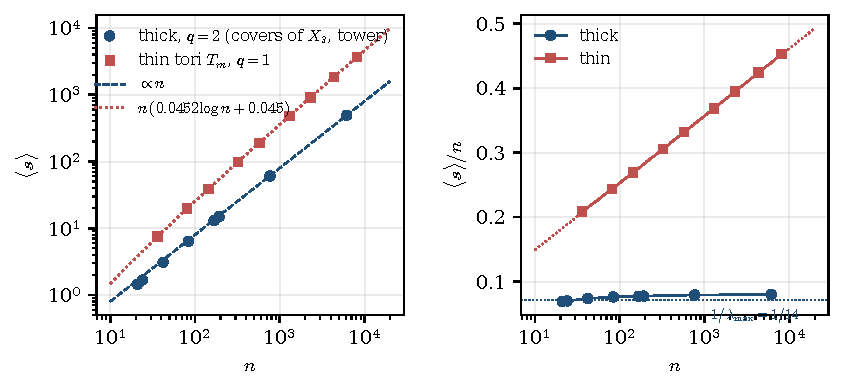
\includegraphics[width=\textwidth]{figures/fig_avalanche_distribution.pdf}
\caption{Exact mean avalanche size $\langle s\rangle=\mathbf 1^{t}G\mathbf 1/(n-1)$ of the vertex
sandpile (sink $=$ vertex $0$, Theorem~\ref{V3P2:thm:mean}), computed by solving the reduced Laplacian
system. Thick, $q=2$: the abelian covers $Y_{21},Y_{24},Y_{42},Y_{84},Y_{168}$ of $X_3$ and the levels
$n=192,768,6144$ of the canonical $2$-tower of Section~\ref{V3P6:sec:cs}. Thin, $q=1$: the tori
$T_m$, $m=6,\dots,90$ ($n=m^{2}$), whose $1$-skeleton is the triangular lattice. Left: $\langle s\rangle$
against $n$ on logarithmic axes, with the line $\propto n$ through the thick family and the fit
$n(a\log n+c)$ through the thin one. Right: $\langle s\rangle/n$, which stays between $0.069$ and $0.080$
on the thick family, as Corollary~\ref{V3P2:cor:linear} predicts ($\ge1/\lambda_{\max}=1/14$), and grows
like $a\log n$ on the thin family, with fitted $a=0.0452$; the triangular-lattice value is
$\sqrt3/(12\pi)=0.0459$, since there $\lambda(k)\approx\frac32|k|^{2}$ and the Brillouin zone has area
$8\pi^{2}/\sqrt3$ (the constant $\frac1{4\pi}$ of Corollary~\ref{V3P2:cor:linear} is that of the square
torus). Drawn by \texttt{code/make\_figures.py}; $\langle s\rangle(Y_{21})=29/20$ is checked there.}
\label{V3P2:fig:avalanche}
\end{figure}

\begin{proposition}[Lyons \cite{Lyons2005}]\label{V3P2:prop:lyons}
If finite $d$-regular graphs $G_j$ converge in the Benjamini--Schramm sense to a transitive
graph $G$, then
$\frac1{|V(G_j)|}\log|\Jac_0(G_j)|\to h(G)=\log d-\sum_{k\ge1}\frac{p_k(o,o)}{k}$, where
$p_k(o,o)$ is the $k$-step return probability of simple random walk on $G$.
\end{proposition}

For quotients $\Gamma_j\backslash B$ with injectivity radius tending to infinity, the limit
graph is the $1$-skeleton of the building. It is transitive, because the Cartwright--Mantero--Steger--Zappa
group acts simply transitively on vertices (Vol.~I--II, Construction~\ref{M-X:con:thick}).
Its entropy $h(B^{(1)})<\log(2(q^{2}+q+1))$ is the ``asymptotic principal exponent'' of the
vertex sandpile groups. We do not compute it. The finite complexes of this volume form a
bounded chain, not a Benjamini--Schramm sequence, and their values
(Table~\ref{V3P2:tab:covers}) are finite-size data only.

\section{Scaling: what can and cannot be claimed}\label{V3P2:sec:scaling}

\begin{proposition}[Critical branching \cite{Harris63}]\label{V3P2:prop:gw}
Let $(Z_t)$ be a Galton--Watson process with offspring mean $1$ and variance
$\sigma^{2}\in(0,\infty)$. Then $\mathbb P(Z_t>0)\sim2/(\sigma^{2}t)$. If the offspring law
is aperiodic, the total progeny $S$ satisfies
$\mathbb P(S=s)\sim(2\pi\sigma^{2})^{-1/2}s^{-3/2}$. Conditionally on survival to time $t$,
$Z_t/t$ converges to an exponential law (Yaglom). Hence the size exponent is $\tau=3/2$, the
duration exponent is $\tau_T=2$, and $s\sim T^{2}$.
\end{proposition}

\begin{conjecture}[Mean-field class]\label{V3P2:conj:mf}
Let $(Y_j)$ be finite quotients of a thick $\Atwo$ building of order $q$ with injectivity
radius $\to\infty$ and $\lambda_2(\Delta_0)$ bounded below. Then, in the scaling window, the
vertex-sandpile avalanche size and duration have the mean-field exponents $\tau=3/2$ and
$\tau_T=2$, with $s\sim T^{2}$.
\end{conjecture}

\emph{Heuristic.} The local limit is a transitive graph of exponential growth on which
simple random walk has spectral radius $<1$. A toppling at depth $r$ from the seed reaches,
with high probability, sites whose earlier history it has not influenced, so the avalanche
is locally a branching process. Criticality of the stationary state (mean offspring $1$)
then gives Proposition~\ref{V3P2:prop:gw}. The same reasoning is known to be exact on the
Bethe lattice \cite{DM90}. The $1$-skeleton, however, contains many triangles (the chambers),
so the tree approximation is uncontrolled. We do not claim a proof.

\begin{remark}[Corrections concerning exponents]\label{V3P2:rem:exponents}
(1) \emph{The dynamic exponent $z$.} Here $z$ is defined by $T\sim L^{z}$ with $L$ a linear
size. On expanders the diameter is $\Theta(\log n)$, so no power law in $L$ is meaningful.
The well-defined replacement is the size--duration exponent $\gamma$ in $s\sim T^{\gamma}$,
conjecturally $\gamma=2$. (2) \emph{The comparison value $1.22$.} The one-dimensional BTW
model has no power-law avalanches at all. The value $\tau\approx1.22$ is an early numerical
estimate for the \emph{two}-dimensional BTW model; later estimates range over roughly
$1.2$--$1.3$, and no value is proved. (3) \emph{Topology.} The divergence from Euclidean
lattices is not topological. The vertex sandpile does not see $b_1(Y)=0$: its graph has
first Betti number $|E|-n+1=6n+1$ for $q=2$. What it sees is expansion, and its rigorous
signature is Corollary~\ref{V3P2:cor:linear}: $\langle s\rangle=\Theta(n)$ against
$\Theta(n\log n)$. (4) \emph{Chambers.} There is no avalanche of chambers to renormalize
(Corollary~\ref{V3P2:cor:nonabelian}).
\end{remark}

\section{The example \texorpdfstring{$Y_{21}$}{Y21}}\label{V3P2:sec:example}

\begin{proposition}[$Y_{21}$ is dense]\label{V3P2:prop:k777}
The $1$-skeleton of $Y_{21}$ is the complete tripartite graph $K_{7,7,7}$. Consequently
$\Tr A_1^{3}=3\cdot7^{3}=1029$, and the $196=343-147$ non-chamber $3$-cycles of Chapter~\ref{chap:V3P1}
(Section~\ref{V3P1:sec:examples}) are all the type-increasing triangles of $K_{7,7,7}$ that
are not chambers.
\end{proposition}

\begin{proof}
Each vertex has $q^{2}+q+1=7$ neighbours of each other type, and there are exactly $7$
vertices of each type. So every pair of vertices of different types is adjacent, and every
choice of one vertex of each type gives a type-increasing $3$-cycle.
\end{proof}

\paragraph{Thresholds.} The threshold of site $i$ is $M_{ii}$, and the largest stable height is
$M_{ii}-1$:
\begin{center}
\begin{tabular}{lcccc}
\toprule
& vertex $\Delta_0$ & edge $\Delta_1$ & chamber $\Delta_2$ & Hecke $\DeltaH$\\
\midrule
threshold, general $q$ & $2(q^{2}+q+1)$ & $q+3$ & $3$ & $q^{3}-1$\\
threshold, $q=2$ & $14$ & $5$ & $3$ & $7$\\
neighbours in support & $14$ & $20$ & $3q=6$ & $14$\\
abelian dynamics & yes & no & no & no\\
\bottomrule
\end{tabular}
\end{center}

\paragraph{Groups.} By Smith forms, recomputed and in agreement with
Vol.~I--II, Ch.~\ref{M-chap:X}:
\begin{align*}
\Jac_0(Y_{21})&=\Z/2\oplus(\Z/14)^{15}\oplus\Z/98\oplus\Z/294,\quad
|\Jac_0|=21\cdot14^{18}=3\cdot2^{18}\cdot7^{19},\\
\Jac_1(Y_{21})&=(\Z/2)^{10}\oplus(\Z/14)^{10}\oplus(\Z/98)^{26}\oplus\Z/2058\oplus\Z/18522,\\
\Jac_2(Y_{21})&=(\Z/2)^{13}\oplus(\Z/14)^{15}\oplus\Z/98\oplus\Z/294 .
\end{align*}
Here $|\Jac_0|$ is the spanning-tree count $N^{k-2}\prod_i(N-n_i)^{n_i-1}=21\cdot14^{18}$ of
$K_{7,7,7}$. Moreover $H_2(Y_{21};\Z)\cong\Z^{20}$ has discriminant $3\cdot7^{29}$, and
Theorem~\ref{V3P2:thm:hodge} reads
$|\Jac_1|=21\cdot(3\cdot2^{18}\cdot7^{19})\cdot|\Jac_2|\cdot3\cdot7^{29}=2^{48}\cdot3^{4}\cdot7^{68}$.
The group exponents are $294=2\cdot3\cdot7^{2}$ for $\Jac_0$ and
$18522=2\cdot3^{3}\cdot7^{3}$ for $\Jac_1$.

\paragraph{Avalanches.} The spectrum of $\Delta_0(K_{7,7,7})$ is $0$, $14^{(18)}$, $21^{(2)}$,
and $K_{7,7,7}$ is vertex-transitive. By Theorem~\ref{V3P2:thm:mean},
\[
\langle s\rangle=\frac{21}{20}\Bigl(\frac{18}{14}+\frac{2}{21}\Bigr)=\frac{29}{20}=1.45 ,
\]
confirmed exactly by solving $\widetilde\Delta_0x=\mathbf 1$, and by Monte Carlo
($2\cdot10^{5}$ additions: $1.45006$). This number says nothing about criticality:
$Y_{21}$ is too dense (degree $14$ on $21$ vertices) to host a scaling regime.

\begin{table}[ht]
\centering\small
\renewcommand{\arraystretch}{1.2}
\begin{tabular}{lcccccc}
\toprule
$Y$ & $n$ & $\lambda_2(\Delta_0)$ & $\lambda_{\max}$ & $\langle s\rangle$ & $[n/\lambda_{\max},\,n/\lambda_2]$ & $\frac1n\log|\Jac_0|$\\
\midrule
$Y_{21}$ & 21 & 14 & 21 & $29/20=1.4500$ & $[1.00,\,1.50]$ & 2.407026\\
$Y_{24}$ & 24 & 13 & 21 & $7031/4186=1.6796$ & $[1.14,\,1.85]$ & 2.426183\\
$Y_{42}$ & 42 & 8.417424 & 21 & $489107/157768=3.1002$ & $[2.00,\,4.99]$ & 2.485136\\
$Y_{84}$ & 84 & 8.417424 & 21 & $6.3933$ & $[4.00,\,9.98]$ & 2.532442\\
$Y_{168}$ & 168 & 8.417424 & 21 & $12.9760$ & $[8.00,\,19.96]$ & 2.560221\\
\bottomrule
\end{tabular}
\medskip
\caption{Vertex sandpiles on the covers of Chapter~\ref{chap:V3P1} (sink $=$ vertex $0$). The values of
$\langle s\rangle$ are exact rationals for $n\le42$ and floating point otherwise. The
entropies for $Y_{84},Y_{168}$ agree with the $\Jac_0$ data of Vol.~I--II,
Ch.~\ref{M-chap:X} to six digits. $\lambda_{\max}=21$ throughout: it comes from the
$\omega$-twisted characters $\omega^{\tau}$, with $A_1+A_2$ eigenvalue $2\operatorname{Re}
(7\omega)=-7$. For comparison, $\log14=2.639057$.}
\label{V3P2:tab:covers}
\end{table}

\section{Verification battery}\label{V3P2:sec:battery}

\begin{table}[ht]
\centering\scriptsize
\renewcommand{\arraystretch}{1.2}
\resizebox{\textwidth}{!}{%
\begin{tabular}{lcl}
\toprule
check & complexes & result\\
\midrule
(S) switching to a Z-matrix: $\Delta_0$ yes; $\Delta_1,U_1$ no; $\Delta_2$ no (thick), yes ($T_6$); $\DeltaH_{xy}\DeltaH_{yx}=-q$ & $Y_{21},Y_{24},Y_{42},T_6$ & exact\\
(S') $\Delta_1$: diagonal $q+3$, entries $\{0,\pm1\}$, $20$ neighbours, $0$ inside chambers & $Y_{21}$ & exact\\
(N) two-site non-abelian example; $300$ random stabilizations: $0$ non-terminating, $113$ order-dependent, $294$ negative & $Y_{21}$ & exact / numeric (seed 1)\\
(K) $1$-skeleton $=K_{7,7,7}$; $\Tr A_1^{3}=1029$ & $Y_{21}$ & exact\\
(H) $|\Jac_1|\operatorname{disc}\ker\Delta_1=n|\Jac_0||\Jac_2|\operatorname{disc}H_2$; $\det\Delta_1=|\Jac_1|$ when $b_1=0$ & $Y_{21},Y_{24},T_6$ & exact\\
(D) $\langle s\rangle$ as exact rationals; Monte Carlo on $Y_{21}$ within $0.02$ & $Y_{21},Y_{24},Y_{42}$ & exact / numeric\\
(E) $\frac1n\log|\Jac_0|$ from spectra; agreement with Vol.~I--II, Ch.~\ref{M-chap:X} for $Y_{168}$ & five covers & numeric $10^{-6}$\\
\bottomrule
\end{tabular}}
\medskip
\caption{Checks run by \texttt{code/v3p2\_verify.py}; the complexes are built by
\texttt{code/a2\_common.py}.}
\label{V3P2:tab:battery}
\end{table}

\section{Scope, residue, corrections}\label{V3P2:sec:scope}

\begin{remark}[Solved, open]\label{V3P2:rem:scope}
\emph{Solved:} the sign obstruction for every higher toppling operator on thick complexes,
and its absence for chambers on thin ones; the Hodge factorization of the orders of the
critical groups; exact avalanche means, their spectral bounds, and the $\Theta(n)$ versus
$\Theta(n\log n)$ dichotomy; the structure of $Y_{21}$. \emph{Open:}
(a) Conjecture~\ref{V3P2:conj:mf};
(b) the entropy $h(B^{(1)})$ of the building's $1$-skeleton, computable in principle from
return probabilities through the spherical Hecke algebra of $(A_1,A_2)$;
(c) whether some non-sign-coherent generalization of chip-firing (a choice of firing cone
for a general nonsingular matrix) gives a meaningful dynamical avatar of $\Jac_1$;
(d) a structural (not merely numerical) relation between $\Jac_1$, $\Jac_0\oplus\Jac_2$ and
$H_2(Y;\Z)$ refining Theorem~\ref{V3P2:thm:hodge};
(e) the analogue of Theorem~\ref{V3P2:thm:sign} for $\Atilde d$, where the same $3$-cycles
exist.
\end{remark}

\begin{remark}[Corrections to the proposed programme]\label{V3P2:rem:corrections}
(1) The toppling rules built from $\Delta_1$ and $\Delta_2$ are not sandpiles: under every
orientation they are not abelian (Theorem~\ref{V3P2:thm:sign},
Corollary~\ref{V3P2:cor:nonabelian}). The ``recurrent configuration group
$\operatorname{Pic}_k$'' does not exist for $k=1,2$, and only the algebraic
$\coker\Delta_k$ remains. (2) $\operatorname{Pic}_k\cong\Z^{|S_k|-1}/\operatorname{im}\Delta_k'$
is the vertex statement. For $k=1$ and $b_1=0$, $\coker\Delta_1$ is finite of order
$\det\Delta_1$ with no reduction, and ``$|\operatorname{Pic}_1|=\det'\Delta_1$'' is a
tautology. The substantive statement is Theorem~\ref{V3P2:thm:hodge}. (3) Avalanche exponents
are not provable on finite complexes. $\tau=3/2$, $\tau_T=2$, $s\sim T^{2}$ are proved for the
branching approximation and conjectured for the sandpile; $z$ in the usual sense is undefined
on expanders. (4) The Euclidean value $1.22$ is a numerical estimate for the $2$D (not $1$D)
BTW model. (5) The divergence from Euclidean lattices is spectral (expansion), not
topological: it is Corollary~\ref{V3P2:cor:linear}, and $b_1(Y)=0$ plays no role in it.
(6) ``Local nontrivial toppling thresholds'' for $Y_{21}$ are $14,5,3,7$. The ``asymptotic
principal exponent'' is read as the growth rate of $|\Jac_0|$, which is
$2.4070$ per vertex on $Y_{21}$. Its limit along Benjamini--Schramm sequences is the entropy
of Proposition~\ref{V3P2:prop:lyons}, which is not computed here.
\end{remark}

\section*{Acknowledgement of provenance and caveats}

Unrefereed. The classical inputs are Dhar's theory of recurrent states \cite{Dhar90}, the
limit theorems for critical Galton--Watson processes \cite{Harris63}, Lyons' entropy theorem
\cite{Lyons2005}, and the Bethe-lattice computation \cite{DM90}, which is cited only for the
heuristic. Everything else is proved here or in Chapter~\ref{chap:V3P1}. The complexes are rebuilt by
\texttt{code/a2\_common.py} independently of the scripts of Vol.~I--II; where the data
overlap, they agree. The bibliographic data of \cite{Dhar90,DM90,Harris63} have been checked against Crossref and zbMATH.

% Volume III, Chapter 3 (drafted as "Chapter 29")
\chapter{Phase Oscillators on Buildings: Chiral Connections, Frustrated Ground States, and Transverse Bifurcations}\label{chap:V3P3}
\chaptermark{Phase Oscillators on Buildings}
\begin{chapterabstract}
The proposed programme asks for a gauge-covariant Kuramoto model on an $\Atwo$ complex, with pairwise
coupling $K_1$ through a connection $A$ of chamber flux $2\pi\alpha_0$ and a triadic chamber
coupling $K_2$ with lag $\Phi$. It then asks for proofs of four claims. (a) The flux breaks
time reversal and forbids static fixed points, forcing a permanent chiral limit cycle. (b) An
Ott--Antonsen reduction closes on the three type classes, and a supercritical Hopf
bifurcation produces a chimera with one class coherent and two incoherent. (c) The Berry phase
of the synchronized cycle is topological. (d) The frequency shift is fixed by the Euler
characteristic and the number of chambers. We prove what is true and correct what is not.

(1) \emph{Chiral connections.} The uniform connection $A^{\alpha}=\frac{2\pi\alpha}{3}\mathbf
1_E$ has flux $2\pi\alpha$ on every chamber of every $\Atwo$ complex. Chiral connections of a
given flux form a torsor under $\Hom(H_1(Y;\Z),U(1))$, which is finite on thick complexes by
Garland rigidity ($64$ classes on $Y_{21}$). The triadic lag $\Phi$ is \emph{not} a gauge
field: the only gauge-covariant triadic term is blind to the flux.

(2) \emph{The flux sector is a gradient flow.} For $K_2=0$ and identical frequencies, the
model is the gradient flow of a frustrated XY energy for every flux. Every trajectory
converges to an equilibrium, all Jacobians are symmetric, and there are no limit cycles and
no Hopf bifurcations. Claim (a) is therefore false. The ground states are the three
\emph{twisted states} $\theta_j=\frac{2\pi m}{3}\tau(j)$; we determine exactly which of them
minimize the energy. The flux produces static persistent currents, not rotation.

(3) \emph{The triadic lag.} For all parameters the twisted states are relative equilibria
rotating at $\Omega=\omega+K_2\sin\Phi$. Their Jacobian is $-c_m\Delta_0$, so its spectrum is
real, stability changes only through a real, $(n-1)$-fold degenerate crossing, and never
through a Hopf bifurcation. On the type-cluster subspace the whole system is a gradient flow
modulo rotation. At every cluster equilibrium the Jacobian splits into $3\times3$ blocks
$M(\lambda)$ indexed by the $\Z/3$-orbits of eigenvalues of $A_1$. On $Y_{21}$ every block is
real. On $Y_{168}$ a stable cluster state can lose stability through a complex pair of a transverse
block; this happens at about a fifth of the losses of stability found, always with multiplicity $21$,
and in every case examined the network then freezes into a locked state instead of a limit cycle.

(4) \emph{Ott--Antonsen and chimeras.} The OA manifold is invariant only for $K_2=0$: the
triadic term is second harmonic in $\theta_j$, and we prove non-closure. For $K_2=0$ we derive
the closed equations for $(r_t,\psi_t)$ and a Lyapunov function that excludes chimeras and
Hopf bifurcations for identical oscillators. For $K_2\ne0$ the chimera of (b) remains
unproved. Numerically it is never the primary instability of a stable cluster state, and it
did not appear in our runs.

(5) \emph{Phases and frequencies.} A rigid rotation has zero geometric phase. The genuine
geometric datum is the monodromy of the twisted states under threading one flux quantum per
chamber. It is the cyclic permutation $\Theta_m\mapsto\Theta_{m+1}$, implemented by the
grading character of Chapter~\ref{chap:V3P1}. The frequency shift is $K_2\langle m_\Delta\rangle_F$, a local
quantity. The identity $D_2=3|F|/\chi(Y)$ holds only for $q=2$; on the thin torus $\chi=0$
while the shift is not. Trees fail for two reasons: every connection on a tree is pure gauge,
and without $2$-cells the dynamics is a gradient flow.
\end{chapterabstract}

\section*{Status of the results}

Every numbered statement is proved. The exceptions are the numerical observations in
Remark~\ref{V3P3:rem:numerics}, Theorem~\ref{V3P3:thm:hopf} and Remark~\ref{V3P3:rem:hopfdyn}, which
are numerical, and two classical inputs: the \L{}ojasiewicz convergence
theorem for analytic gradient flows \cite{Loj63} and LaSalle's invariance principle
\cite{LaSalle60}. The Ott--Antonsen equations are derived here in the form used, together with
their failure for $K_2\ne0$. All finite identities, and the numerical statements, were checked
by \texttt{code/v3p3\_verify.py} (Table~\ref{V3P3:tab:battery}).

Notation follows Chapters~\ref{chap:V3P1}--\ref{chap:V3P2}. $Y$ is a finite $\Atwo$ complex satisfying (L) for some
$q\ge1$. For $q=1$ this means the thin tori, whose links are hexagons. Put
$\kappa=q^{2}+q+1$. Then every vertex has $\kappa$ out-neighbours (type $+1$) and $\kappa$
in-neighbours (type $-1$), every edge lies in $q+1$ chambers, every vertex lies in
$D_2=\kappa(q+1)$ chambers, and $|E|=\kappa n$, $3|F|=nD_2$. Edges are oriented
$j\to k$ with $\tau(k)=\tau(j)+1$, chambers are oriented $a\to b\to c\to a$, and
$P_t$ is the projection onto the class $V_t=\tau^{-1}(t)$, of size $n/3$. As in Vol.~I--II,
Definition~\ref{M-X:def:a2}, $A_1$ is normal: $A_1A_1^{t}=A_1^{t}A_1$.

\section{The model and its gauge structure}\label{V3P3:sec:model}

\begin{definition}[Connections and flux]\label{V3P3:def:conn}
A \emph{connection} is a function $A$ on ordered adjacent pairs with $A_{kj}=-A_{jk}$, taken
modulo $2\pi$. Equivalently, it is a $1$-cochain $A\in C^{1}(Y;\R/2\pi\Z)$ on the oriented
edges. Its \emph{flux} is the $2$-cochain $\delta A$, with
$(\delta A)(a,b,c)=A_{ab}+A_{bc}+A_{ca}$. $A$ is \emph{chiral of flux $2\pi\alpha$} if
$\delta A=2\pi\alpha$ on every (type-increasingly oriented) chamber. A \emph{gauge
transformation} $\chi\in C^{0}(Y;\R)$ acts by $\theta_j\mapsto\theta_j+\chi_j$,
$A_{jk}\mapsto A_{jk}-(\chi_k-\chi_j)$. It preserves the link variables
$\varphi_{jk}=\theta_k-\theta_j+A_{jk}$ and the flux.
\end{definition}

\begin{proposition}[Chiral connections]\label{V3P3:prop:chiral}
\begin{enumerate}
\item[(i)] For every $\alpha\in\R$ the uniform connection $A^{\alpha}$, equal to
$a=\frac{2\pi\alpha}{3}$ on every oriented edge, is chiral of flux $2\pi\alpha$.
\item[(ii)] $A^{\alpha+1}$ is gauge equivalent to $A^{\alpha}$, via the type gauge
$\chi=\frac{2\pi}{3}\tau$. In particular $A^{m}$ is pure gauge for $m\in\Z$.
\item[(iii)] The gauge classes of chiral connections of flux $2\pi\alpha$ form a torsor under
$\Hom(H_1(Y;\Z),U(1))$. If $q\ge2$, this group is finite of order $|H_1(Y;\Z)|$
(Theorem~\ref{V3P1:thm:garland}). On $Y_{21}$, where $H_1=(\Z/2)^{6}$, there are $64$ classes.
\end{enumerate}
\end{proposition}

\begin{proof}
(i) Each chamber has three oriented edges. (ii) $\chi_k-\chi_j=\frac{2\pi}{3}$ on every edge
$j\to k$. (iii) If $A,A'$ are both chiral of flux $2\pi\alpha$, then $\delta(A-A')=0$, so
$A-A'$ is a flat connection. Modulo gauge, flat connections form $H^{1}(Y;\R/2\pi\Z)$, which
equals $\Hom(H_1(Y;\Z),\R/2\pi\Z)$ by the universal coefficient theorem, because $\R/2\pi\Z$ is
divisible. When $b_1=0$ this is the Pontryagin dual of the finite group $H_1$.
\end{proof}

So the constant flux imposes no quantization. The $2$-cochain $\mathbf 1_F=\frac13\delta\mathbf
1_E$ is exact, and every integral $2$-cycle has zero chamber sum.

\begin{definition}[The model]\label{V3P3:def:model}
For $\omega\in\R$, $K_1,K_2\in\R$, $\alpha,\Phi\in\R$ and $a=\frac{2\pi\alpha}{3}$:
\begin{equation}\label{V3P3:eq:model}
\dot\theta_j=\omega_j+\frac{K_1}{2\kappa}\sum_{k\sim j}\sin(\theta_k-\theta_j+A^{\alpha}_{jk})
+\frac{K_2}{D_2}\sum_{\{j,k,l\}\in F}\sin(\theta_k+\theta_l-2\theta_j+\Phi).
\end{equation}
Unless stated otherwise, $\omega_j=\omega$ for all $j$. Write $\varphi_e$ for the link variable on a
type-increasing edge $e$, and for a chamber $\Delta$ with corner $j$ write
$x^{\Delta}_j=\theta_k+\theta_l-2\theta_j$ and $m_\Delta=\frac13\sum_{j\in\Delta}
\sin(x^{\Delta}_j+\Phi)$.
\end{definition}

\begin{remark}[The triadic lag is not a gauge field]\label{V3P3:rem:lag}
The pairwise term of \eqref{V3P3:eq:model} is gauge covariant, but the triadic term with a
corner-independent $\Phi$ is not: under $\chi$ its argument shifts by
$\chi_k+\chi_l-2\chi_j$. The covariant triadic term built from the connection is
$\sin(\varphi_{jk}+\varphi_{jl})$. Its three corner arguments sum to
$\sum(\varphi_{jk}+\varphi_{kj})=0$, whatever the flux, and in the gauge $A^{\alpha}$ it
equals the $\Phi=0$ term of \eqref{V3P3:eq:model}, because $A_{jk}+A_{jl}=a-a=0$. Thus the
flux $\alpha$ and the lag $\Phi$ are independent parameters. $\Phi$ is a Sakaguchi-type lag
\cite{SK86} on the triadic coupling of Skardal--Arenas type \cite{SA19}, not a curvature.
\end{remark}

\section{Symmetries and the gradient sector}\label{V3P3:sec:gradient}

The model is invariant under the global rotation $\theta\mapsto\theta+c\mathbf 1$. The
conjugation $C\colon\theta\mapsto-\theta$ maps the parameters $(\omega,\alpha,\Phi)$ to
$(-\omega,-\alpha,-\Phi)$. Since $\alpha$ matters only modulo $1$
(Proposition~\ref{V3P3:prop:chiral}(ii)), the flux is $C$-invariant exactly when
$\alpha\in\frac12\Z$. This is the precise sense in which the flux is ``T-odd''.

\begin{proposition}[Frequency sum rule]\label{V3P3:prop:sum}
For every state $\theta$ and arbitrary $\omega_j$,
\[
\frac1n\sum_j\dot\theta_j=\bar\omega+K_2\,\langle m_\Delta\rangle_F,\qquad
\langle m_\Delta\rangle_F=\frac1{|F|}\sum_{\Delta\in F}m_\Delta .
\]
Hence every frequency-locked state has $|\Omega-\bar\omega|\le|K_2|$, and for $K_2=0$ its
frequency is $\bar\omega$ whatever the flux.
\end{proposition}

\begin{proof}
Each edge contributes $\sin\varphi_e-\sin\varphi_e=0$ to the pairwise part, because all
degrees are equal to $2\kappa$. Each chamber contributes $3m_\Delta$ to the triadic part, and
$nD_2=3|F|$.
\end{proof}

\begin{theorem}[The flux sector is a gradient flow]\label{V3P3:thm:gradient}
Let $G$ be any finite graph and $A$ any connection on it. Suppose $K_2=0$ and
$\omega_j=\omega$. In the frame rotating at $\omega$, the model
$\dot\theta_j=\frac{K_1}{\deg j}\sum_{k\sim j}\sin\varphi_{jk}$ is the gradient flow of
\[
V_A(\theta)=-K_1\sum_{e}\cos\varphi_e
\]
for the metric $\sum_j\deg(j)\,d\theta_j^{2}$. Consequently:
\begin{enumerate}
\item[(i)] every trajectory converges to a single equilibrium;
\item[(ii)] at every equilibrium the Jacobian is self-adjoint for this metric, so its spectrum
is real;
\item[(iii)] there is no periodic orbit other than equilibria, and no Hopf bifurcation, for any
flux.
\end{enumerate}
In particular, in the model \eqref{V3P3:eq:model} with $K_2=0$ a nonzero flux does not
prevent static fixed points and does not force rotation.
\end{theorem}

\begin{proof}
$\partial V_A/\partial\theta_j=-K_1\sum_{k\sim j}\sin\varphi_{jk}$, because
$\varphi_{kj}=-\varphi_{jk}$. So $\dot\theta_j=-\deg(j)^{-1}\partial_jV_A$. $V_A$ is real
analytic on the compact torus, so by \L{}ojasiewicz \cite{Loj63} every trajectory has finite
length and converges. The Jacobian is $-g^{-1}\operatorname{Hess}V_A$, which is self-adjoint
for $g$. Along a non-constant orbit $V_A$ strictly decreases, which excludes periodic orbits.
\end{proof}

\begin{lemma}[Triangle lemma]\label{V3P3:lem:triangle}
Let $S\in[-\pi,\pi]$. On $\{x\in\R^{3}:x_1+x_2+x_3\equiv S\bmod2\pi\}$,
$\max\sum_i\cos x_i=3\cos(S/3)$. For $|S|<\pi$ the maximum is attained only at
$x_i\equiv S/3$.
\end{lemma}

\begin{proof}
At a critical point the Lagrange condition gives $\sin x_1=\sin x_2=\sin x_3$, so each
$x_i\in\{u,\pi-u\}$ modulo $2\pi$. If all three equal $u$ (or all equal $\pi-u$), the value is
$3\cos\frac{S+2\pi k}{3}$ for some $k$, and it is largest for $k=0$ because $|S|\le\pi$. If the
two values are mixed, then either $(u,u,\pi-u)$ with $u\equiv S-\pi$, of value $\cos u$, or
$(u,\pi-u,\pi-u)$ with $u\equiv-S$, of value $-\cos u$; both equal $-\cos S$. Put
$c=S/3\in[-\frac\pi3,\frac\pi3]$. Then
$3\cos c-(-\cos3c)=4\cos^{3}c>0$.
\end{proof}

\begin{theorem}[Frustrated ground states]\label{V3P3:thm:ground}
Let $K_1>0$ and $K_2=0$. Write $\alpha=\operatorname{round}(\alpha)+\beta$ with
$\beta\in[-\frac12,\frac12]$, and define the \emph{twisted states}
$\Theta_m=\frac{2\pi m}{3}\tau$, $m\in\Z/3$. Then
\[
\min V_{A^{\alpha}}=-K_1|E|\cos\tfrac{2\pi\beta}{3}.
\]
The minimizers are the rotations of $\Theta_{m_*}$, $m_*\equiv-\operatorname{round}(\alpha)$.
At a minimizer every type-increasing edge carries the same link variable $\frac{2\pi\beta}{3}$,
and hence the static current $K_1\sin\frac{2\pi\beta}3$. For $|\beta|<\frac12$ the minimizer
is unique up to rotation. For $\alpha\in\frac12+\Z$ there are exactly two minimizers, with link
variables $\pm\frac\pi3$, and $C$ exchanges them.
\end{theorem}

\begin{proof}
Around each chamber $\varphi_{ab}+\varphi_{bc}+\varphi_{ca}=3a=2\pi\alpha\equiv2\pi\beta$,
because the $\theta$-differences cancel. Each edge lies in $q+1$ chambers, so by
Lemma~\ref{V3P3:lem:triangle}
\[
\sum_e\cos\varphi_e=\frac1{q+1}\sum_{\Delta}\sum_{e\subset\Delta}\cos\varphi_e
\le\frac{3|F|}{q+1}\cos\tfrac{2\pi\beta}3=|E|\cos\tfrac{2\pi\beta}3 .
\]
On $\Theta_m$ every link variable is $\frac{2\pi(m+\alpha)}{3}$, which gives equality for
$m=m_*$. If $|\beta|<\frac12$, equality forces $\varphi_e\equiv\frac{2\pi\beta}3$ on every
edge. Then $\theta_k-\theta_j\equiv\frac{2\pi m_*}{3}$ along every edge $j\to k$, so $\theta$ is
a rotation of $\Theta_{m_*}$ ($Y$ is connected). At $|\beta|=\frac12$, equality forces each
chamber to carry $\frac\pi3$ on all three edges or $-\frac\pi3$ on all three. Two chambers
sharing an edge agree. $Y$ is gallery connected, because it is connected and its links are
connected. So the value is the same everywhere, and $\theta$ is a rotation of one of the two
twisted states with link variables $\pm\frac\pi3$. $C$ reverses link variables, so it exchanges
them.
\end{proof}

\section{Twisted states and the triadic lag}\label{V3P3:sec:twisted}

\begin{theorem}[Twisted states for all parameters]\label{V3P3:thm:twisted}
For all $K_1,K_2,\alpha,\Phi$ and $m\in\Z/3$, the state $\Theta_m+\Omega t$ with
$\Omega=\omega+K_2\sin\Phi$ is a solution of \eqref{V3P3:eq:model}. The Jacobian at $\Theta_m$ is
\[
J_m=-c_m\,\Delta_0,\qquad
c_m=\frac{K_1\cos\frac{2\pi(m+\alpha)}3+2K_2\cos\Phi}{2\kappa}.
\]
Its eigenvalues are $-c_m\lambda_i(\Delta_0)$. $\Theta_m$ is linearly stable modulo rotation
if and only if $c_m>0$. When $c_m$ changes sign, all $n-1$ transverse eigenvalues cross zero
together, along the real axis. In particular no Hopf bifurcation ever occurs at a twisted
state.
\end{theorem}

\begin{proof}
On $\Theta_m$ every link variable is $\pm\frac{2\pi(m+\alpha)}{3}$, and the pairwise
contributions from out- and in-neighbours cancel. Every triadic argument is
$\frac{2\pi m}{3}(\tau_k+\tau_l-2\tau_j)+\Phi=2\pi m+\Phi$. Differentiating the pairwise term
gives $-\frac{K_1}{2\kappa}\cos\frac{2\pi(m+\alpha)}{3}\Delta_0$. For the triadic term,
$\partial_{\theta_k}$ of the $j$-th equation is $\frac{K_2}{D_2}\cos\Phi$ times the number
$q+1$ of chambers containing $j$ and $k$, and $\partial_{\theta_j}$ is $-2K_2\cos\Phi$. Since
$D_2=\kappa(q+1)$, the triadic part is $\frac{K_2\cos\Phi}{\kappa}(A_1+A_2-2\kappa
I)=-\frac{K_2\cos\Phi}{\kappa}\Delta_0$.
\end{proof}

\begin{corollary}[Multistability]\label{V3P3:cor:bistable}
Let $K_2=0$ and $K_1>0$. $\Theta_m$ is stable iff the distance from $m+\alpha$ to $3\Z$ is less
than $\frac34$. Two twisted states are stable exactly when the fractional part of $\alpha$
lies in $(\frac14,\frac34)$, and otherwise only the ground state is. Varying $\alpha$ therefore
produces hysteresis.
\end{corollary}

\paragraph{The type-cluster subspace.} If $\omega_j=\omega$, the subspace
$\{\theta_j=\psi_{\tau(j)}\}$ is invariant: a vertex of type $t$ sees $\kappa$ neighbours of
types $t\pm1$, and each of its chambers has one vertex of each type. With
$d_t=\psi_{t+1}-\psi_t$ (indices mod $3$) the reduced equations are
\begin{equation}\label{V3P3:eq:cluster}
\dot\psi_t=\omega+\tfrac{K_1}{2}\bigl[\sin(d_t+a)-\sin(d_{t-1}+a)\bigr]+K_2\sin(d_t-d_{t-1}+\Phi).
\end{equation}

\begin{theorem}[Gradient structure modulo rotation]\label{V3P3:thm:clustergrad}
Put $U(\psi)=-\frac{K_1}2\sum_t\cos(d_t+a)-\frac{K_2}3\sum_t\cos(d_t-d_{t-1}+\Phi)$. Then
\eqref{V3P3:eq:cluster} reads
$\dot\psi=\omega\mathbf 1-\nabla U+\bar m(\psi)\mathbf 1$ with
$\bar m=\frac{K_2}3\sum_t\sin(d_t-d_{t-1}+\Phi)$. Modulo rotation it is therefore the
gradient flow of $U$. Every cluster trajectory converges to a relative equilibrium, the reduced
Jacobian is symmetric, and there are no periodic orbits or Hopf bifurcations inside the
cluster subspace. For the full network,
\[
\dot\theta=\omega\mathbf 1-\nabla\Bigl(\tfrac{1}{2\kappa}V_{A^{\alpha}}+\tfrac{K_2}{D_2}
\sum_\Delta W_\Delta\Bigr)+\tfrac{K_2}{D_2}\sum_{\Delta}m_\Delta(\theta)\,\mathbf 1_\Delta ,
\qquad W_\Delta=-\tfrac13\sum_{j\in\Delta}\cos(x^{\Delta}_j+\Phi),
\]
so the only non-gradient part is the \emph{chamber drive} $\sum_\Delta m_\Delta\mathbf
1_\Delta$. It is parallel to $\mathbf 1$ whenever all $m_\Delta$ are equal.
\end{theorem}

\begin{proof}
For one chamber,
$-\partial_{\theta_s}W_\Delta=\sin(x^{\Delta}_s+\Phi)-m_\Delta$, because
$\partial x^{\Delta}_j/\partial\theta_s$ is $-2$ for $j=s$ and $1$ otherwise. Summing over chambers
gives the decomposition. On the cluster subspace all $m_\Delta$ equal $\bar m/K_2$, and
$\sum_\Delta\mathbf 1_\Delta=D_2\mathbf 1$. The reduced flow on $T^{3}/S^{1}$ is then the
gradient of $U$, and the \L{}ojasiewicz argument of Theorem~\ref{V3P3:thm:gradient} applies.
\end{proof}

\begin{theorem}[Block decomposition at cluster equilibria]\label{V3P3:thm:blocks}
Let $\psi$ be an equilibrium of \eqref{V3P3:eq:cluster} and $\theta=\psi\circ\tau$. Put
$p_t=\frac{K_1}{2\kappa}\cos(d_t+a)$ and $c_t=\frac{K_2}{\kappa}\cos(d_t-d_{t-1}+\Phi)$, and
\[
\alpha_t=p_t+c_t,\qquad \gamma_t=p_{t-1}+c_t,\qquad \sigma_t=\kappa(\alpha_t+\gamma_t).
\]
Then $J=-\sum_t\sigma_tP_t+\sum_tP_t(\alpha_tA_1+\gamma_tA_2)$, and
$\C^{n}=W_0\oplus\bigoplus_{[\lambda]}W_{[\lambda]}$ is a $J$-invariant decomposition. Here
$W_0=\ker A_1$, and $W_{[\lambda]}=E_\lambda\oplus E_{\omega\lambda}\oplus
E_{\omega^{2}\lambda}$ runs over the $\Z/3$-orbits of nonzero eigenvalues of $A_1$, with
$\omega=e^{2\pi i/3}$. On $W_0$, $J$ acts as $-\sigma_t$ on $W_0\cap\C^{V_t}$. On
$W_{[\lambda]}$ it acts as $M(\lambda)\otimes I_{\dim E_\lambda}$, where
\[
M(\lambda)=\begin{pmatrix}-\sigma_0&\alpha_0\lambda&\gamma_0\bar\lambda\\
\gamma_1\bar\lambda&-\sigma_1&\alpha_1\lambda\\ \alpha_2\lambda&\gamma_2\bar\lambda&-\sigma_2
\end{pmatrix}.
\]
The orbit of $\lambda=\kappa$ is the tangent space of the cluster subspace, and $M(\kappa)$ is
the Jacobian of \eqref{V3P3:eq:cluster}. The rates $\sigma_t$ are the mean-field transverse
rates of the classes.
\end{theorem}

\begin{proof}
The entries of $J$ follow as in Theorem~\ref{V3P3:thm:twisted}. Row $j\in V_t$ has $\alpha_t$ at
each out-neighbour, $\gamma_t$ at each in-neighbour, and $-\sigma_t$ on the diagonal, because
rows sum to zero. Let $D_1=\operatorname{diag}(\omega^{-\tau})$. Then $D_1A_1D_1^{-1}=\omega
A_1$ (Proposition~\ref{V3P1:prop:grading}), so $D_1$ permutes the eigenspaces within an orbit
and $P_t=\frac13\sum_k\omega^{kt}D_1^{k}$ preserves $W_{[\lambda]}$ and $W_0$. $A_1$ is
normal, so $A_2=A_1^{*}$ acts as $\bar\lambda$ on $E_\lambda$. For $v\in E_\lambda$ we have
$A_1P_sv=P_{s-1}A_1v=\lambda P_{s-1}v$ and $A_2P_sv=\bar\lambda P_{s+1}v$. If $P_sv=0$ for one
$s$, these relations force $v=0$, since $\lambda\neq0$. So $\{P_sv_i\}$, for an orthonormal
basis $(v_i)$ of $E_\lambda$, is a basis of $W_{[\lambda]}$, and
$J(P_sv)=-\sigma_sP_sv+\alpha_{s-1}\lambda P_{s-1}v+\gamma_{s+1}\bar\lambda P_{s+1}v$, which
is the stated matrix. On $W_0$ both $A_1$ and $A_2$ vanish.
\end{proof}

\begin{corollary}\label{V3P3:cor:Y21real}
On $Y_{21}$ the Jacobian at every type-cluster equilibrium has real spectrum. So no Hopf
bifurcation occurs at any cluster state of $Y_{21}$.
\end{corollary}

\begin{proof}
The $1$-skeleton is $K_{7,7,7}$ (Proposition~\ref{V3P2:prop:k777}), so
$A_1=C_3\otimes J_7$, with spectrum $7\{1,\omega,\omega^{2}\}$ and $0^{(18)}$. The only block is
$M(7)$, whose spectrum is that of the reduced cluster Jacobian, and this is real by
Theorem~\ref{V3P3:thm:clustergrad}. The remaining eigenvalues are the real numbers $-\sigma_t$.
\end{proof}

On complexes where $A_1$ has nontrivial eigenvalue orbits, $M(\lambda)$ can have complex
eigenvalues. On $Y_{168}$ this happened at $6$ of the equilibria sampled in line (B) of
Table~\ref{V3P3:tab:battery}. A Hopf bifurcation \emph{transverse} to the cluster subspace is
therefore not excluded in general. Section~\ref{V3P3:sec:hopf} shows that it occurs on $Y_{168}$, with
multiplicity $21$ forced by the symmetry, and that the resulting loss of stability is hard.

\section{Mean field and Ott--Antonsen reduction}\label{V3P3:sec:oa}

Replace neighbour sums by class averages $Z_t=r_te^{i\psi_t}=\frac3n\sum_{j\in
V_t}e^{i\theta_j}$, and the pair sum over chambers by $Z_{t+1}Z_{t-1}$. For $j\in V_t$ this
gives
\begin{equation}\label{V3P3:eq:mf}
\dot\theta_j=\omega_j+\operatorname{Im}\bigl(H_te^{-i\theta_j}\bigr)+\operatorname{Im}\bigl(G_te^{-2i\theta_j}\bigr),
\quad H_t=\tfrac{K_1}2\bigl(e^{ia}Z_{t+1}+e^{-ia}Z_{t-1}\bigr),\quad G_t=K_2e^{i\Phi}Z_{t+1}Z_{t-1}.
\end{equation}
On $Y_{21}=K_{7,7,7}$ the pairwise part is \emph{exact}, because every vertex is adjacent to
all of the other two classes. The triadic part is not exact: a vertex lies in $21$ of the $49$
possible cross-class pairs.

For a continuum of oscillators in each class with frequency density $g$, the Ott--Antonsen
ansatz takes the density of class $t$ to be
$f_t=\frac{g(\omega)}{2\pi}\bigl[1+\sum_{n\ge1}(z_t^{n}e^{-in\theta}+\bar z_t^{n}e^{in\theta})\bigr]$,
with $|z_t|<1$ and $z_t=z_t(\omega,\cdot)$ \cite{OA08}.

\begin{proposition}[Closure and non-closure]\label{V3P3:prop:oa}
For the velocity field of \eqref{V3P3:eq:mf}, the continuity equation for the Fourier
coefficient $c_n$ of $e^{-in\theta}$, evaluated on the ansatz, reads
\begin{align*}
\dot z&=i\omega z+\tfrac12(H-\bar Hz^{2})+\tfrac12(G\bar z-\bar Gz^{3})&&(n=1),\\
\dot z&=i\omega z+\tfrac12(H-\bar Hz^{2})+\tfrac12(Gz^{-1}-\bar Gz^{3})&&(n\ge2).
\end{align*}
The ansatz is therefore invariant if and only if $G_t\equiv0$, i.e.\ $K_2=0$. For $K_2=0$ and
a Lorentzian $g$ of centre $\omega_0$ and width $\Delta\ge0$, the class order parameters obey
\[
\dot r_t=-\Delta r_t+\tfrac{K_1(1-r_t^{2})}4\bigl[r_{t+1}\cos(\psi_{t+1}-\psi_t+a)+r_{t-1}\cos(\psi_{t-1}-\psi_t-a)\bigr],
\]
\[
\dot\psi_t=\omega_0+\tfrac{K_1(1+r_t^{2})}{4r_t}\bigl[r_{t+1}\sin(\psi_{t+1}-\psi_t+a)+r_{t-1}\sin(\psi_{t-1}-\psi_t-a)\bigr].
\]
\end{proposition}

\begin{proof}
$\dot c_n=in\omega c_n+\frac n2(Hc_{n-1}-\bar Hc_{n+1}+Gc_{n-2}-\bar Gc_{n+2})$, with
$c_0=1$, $c_n=z^{n}$ and $c_{-n}=\bar z^{n}$. For $n=1$ the term $c_{-1}=\bar z$ appears; for
$n\ge2$ it is $z^{n-2}$. The two equations agree iff $G(\bar z-z^{-1})=0$, i.e.\ $G=0$ or
$|z|=1$. For $G=0$, closing the contour in the half plane where $z(\omega)$ is analytic gives
$Z_t=z_t(\omega_0+i\Delta)$ and $\dot Z_t=(i\omega_0-\Delta)Z_t+\frac12(H_t-\bar H_tZ_t^{2})$.
Taking real and imaginary parts of $\dot Z_te^{-i\psi_t}$ gives the polar form.
\end{proof}

\begin{theorem}[No gauge chimera]\label{V3P3:thm:nochimera}
Let $K_2=0$, $K_1\ne0$ and $\Delta=0$ (identical oscillators), and let
$V(Z)=-\frac12\sum_t\operatorname{Re}(\bar Z_tH_t)$. Along the reduced system of
Proposition~\ref{V3P3:prop:oa},
\[
\dot V\le-\tfrac12\sum_t|H_t|^{2}(1-r_t^{2})\le0 .
\]
Every $\omega$-limit point therefore satisfies, for each $t$, either $H_t=0$, or $r_t=1$ and
$H_t\bar Z_t\in\R$. Consequently:
\begin{enumerate}
\item[(i)] no $\omega$-limit point has $r_0=1>r_1,r_2$ (or any rotation of this);
\item[(ii)] a class with $r_t<1$ at an $\omega$-limit point feels zero field, so it does not
drift: all limit sets are relative equilibria rotating at $\omega_0$;
\item[(iii)] there are no periodic orbits other than rigid rotations, and no Hopf
bifurcation.
\end{enumerate}
The same holds for the finite network by Theorem~\ref{V3P3:thm:gradient}.
\end{theorem}

\begin{proof}
$V=-\frac12Z^{*}WZ$ with $W$ Hermitian, $W_{t,t+1}=\frac{K_1}2e^{ia}$. So $\dot
V=-\operatorname{Re}\sum_t\bar{\dot Z}_tH_t$. Substituting $\dot
Z_t=i\omega_0Z_t+\frac12(H_t-\bar H_tZ_t^{2})$, the $\omega_0$-term is
$\omega_0\operatorname{Im}(Z^{*}WZ)=0$, and
$\dot V=-\frac12\sum_t\bigl(|H_t|^{2}-\operatorname{Re}\bigl((H_t\bar Z_t)^{2}\bigr)\bigr)$,
where $|\operatorname{Re}(w^{2})|\le|w|^{2}$ and $|H_t\bar Z_t|^{2}=|H_t|^{2}r_t^{2}$. Equality
requires, for each $t$, either $H_t=0$, or $r_t=1$ and $(H_t\bar Z_t)^{2}\ge0$. The closed polydisc is invariant,
since $\frac{d}{dt}|Z_t|^{2}=(1-|Z_t|^{2})\operatorname{Re}(\bar Z_tH_t)$. LaSalle
\cite{LaSalle60} gives the first claim. For (i): $H_1=0$ means $e^{ia}Z_2=-e^{-ia}Z_0$, so
$r_2=r_0=1$. For (ii): if $H_t=0$ then $\dot Z_t=i\omega_0Z_t$. For (iii): on a periodic
orbit $V$ is constant, so the orbit lies in the LaSalle set, where the motion is rigid
rotation by (ii).
\end{proof}

\begin{remark}[What is and is not known about chimeras]\label{V3P3:rem:chimera}
Chimeras in the sense of \cite{KB02,AMSW08}, a coherent population beside a drifting one,
need a non-gradient coupling. With the gauge coupling alone they are impossible
(Theorems~\ref{V3P3:thm:gradient}, \ref{V3P3:thm:nochimera}). The triadic lag is the only
non-gradient ingredient of \eqref{V3P3:eq:model}, and its second harmonic removes the OA
closure (Proposition~\ref{V3P3:prop:oa}). For $\Delta>0$ we have no Lyapunov function, and
the question is open. Theorem~\ref{V3P3:thm:blocks} gives the exact criterion for the
\emph{onset} of a type-selective state. At a cluster equilibrium that is stable within the
cluster subspace, class $t$ desynchronizes first iff $\sigma_t<0$ while the other $\sigma_s>0$
(on $Y_{21}$; on other complexes the blocks $M(\lambda)$ must also be stable).
\end{remark}

\begin{remark}[Numerical observations]\label{V3P3:rem:numerics}
(1) We sampled $1500$ random parameter sets $(K_1=\pm1,\ K_2\in[-2,2],\ a,\Phi)$. Among the
$2196$ cluster equilibria found that are stable within the cluster subspace, none had
exactly one class with $\sigma_t>0$. The pattern of the proposed programme ($r_0\approx1$, classes
$1,2$ incoherent) is therefore never the primary instability. The observed pattern is the
opposite: one unstable class, in $124$ cases.
(2) Take $(K_1,K_2,a,\Phi)=(1,-1.99322,-1.01389,-0.06786)$ at the equilibrium
$\psi=(0,1.66481,2.08094)$, where $\sigma=(3.3251,-0.1916,3.2556)$. Started there, class $1$
breaks up, and the network settles into a \emph{frozen} state with a common frequency: on
$Y_{21}$, $r=(1,0.7463,1)$ and $\Omega=1.18831$; on $Y_{168}$, $r=(0.9917,0.9001,0.9909)$ and
$\Omega=1.29345$. This is not a chimera.
(3) An exploratory search on $Y_{168}$ (120 random parameter sets and initial conditions, not
part of the battery) found non-locked states only for $|K_2|\gtrsim1.4$, of two kinds. In
\emph{solitary} states at most two oscillators drift. In \emph{disordered} states most
oscillators of \emph{every} class drift: in the run kept in the battery, $53,52,55$ of the $56$
per class. We found no state in which one class is coherent while the other two are
macroscopically incoherent.
(4) Finite populations ($3\times3000$) started on the OA manifold stay on it for $K_2=0$ up to
sampling error ($|Z_2-Z_1^{2}|\le0.013$). For $K_2=1$ they leave it ($|Z_2-Z_1^{2}|$ reaches
$0.36$).
\end{remark}

\section{Frequency shift and geometric phase}\label{V3P3:sec:berry}

\begin{theorem}[Frequency shift]\label{V3P3:thm:shift}
On every frequency-locked state, $\Omega-\omega=K_2\langle m_\Delta\rangle_F$. On the
twisted states the shift is $\Delta\Omega=K_2\sin\Phi$, independent of $K_1$, $\alpha$, $q$,
$n$, $|F|$ and $\chi(Y)$. If the triadic sum in \eqref{V3P3:eq:model} is not normalized by
$D_2$, the shift becomes $D_2K_2\sin\Phi$ with $D_2=3|F|/n=(q+1)(q^{2}+q+1)$, a count read off
the vertex link.
\end{theorem}

\begin{proof}
Proposition~\ref{V3P3:prop:sum} and Theorem~\ref{V3P3:thm:twisted}.
\end{proof}

\begin{remark}[The Euler characteristic does not enter]\label{V3P3:rem:euler}
Under (L), $\chi(Y)=n-|E|+|F|=n\bigl(1+\frac{\kappa(q-2)}{3}\bigr)$. For $q=2$ this is $n$
($|E|=|F|=7n$), so $D_2=3|F|/\chi(Y)$. That identity is the only sense in which ``the shift
is set by $\chi$ and the number of chambers'' holds, and it is a coincidence of $q=2$. On the
thin torus $T_6$, $\chi=0$ while $D_2=6$ and $\Delta\Omega=K_2\sin\Phi\ne0$. Both $|F|$ and
$\chi$ are multiplied by the degree under coverings, and $\Delta\Omega$ is a local
quantity.
\end{remark}

\begin{proposition}[Geometric phase of a rigid rotation]\label{V3P3:prop:berry}
Let $\theta(t)=\theta^{*}+\Omega t\mathbf 1$ be a relative equilibrium, $\Omega\ne0$, and
$u(t)=n^{-1/2}(e^{i\theta_j(t)})_j$. Over one period $T=2\pi/\Omega$, the total phase
$\arg\langle u(0),u(T)\rangle$ equals the dynamical phase
$\int_0^{T}\operatorname{Im}\langle u,\dot u\rangle\,dt=2\pi$. The Aharonov--Anandan
geometric phase is therefore $0$.
\end{proposition}

\begin{proof}
$u(t)=e^{i\Omega t}u(0)$, so its projective class is constant and encloses no area in
$\C\PP^{n-1}$.
\end{proof}

\begin{proposition}[Flux-threading monodromy]\label{V3P3:prop:monodromy}
Consider the loop $\alpha\mapsto\alpha+1$ in the circle of chiral fluxes, with fibres
identified by the gauge $\chi=\frac{2\pi}3\tau$ of
Proposition~\ref{V3P3:prop:chiral}(ii). The continuation of $\Theta_m$ over the loop ends at
$\Theta_{m+1}$. So the monodromy of the triple $\{\Theta_0,\Theta_1,\Theta_2\}$ is the cyclic
permutation, implemented by multiplying $e^{i\theta}$ by the grading character
$\omega^{\tau}=D_1^{-1}$ of Proposition~\ref{V3P1:prop:grading}. The three states are
pairwise orthogonal ($\sum_j\omega^{\tau(j)}=0$), so the monodromy is a permutation, not a
phase. It has order $3$. If $K_2=0$ and $K_1>0$, the branch on which $m+\alpha$ runs from
$-\frac12$ to $\frac12$ stays linearly stable over the whole loop
(Corollary~\ref{V3P3:cor:bistable}).
\end{proposition}

\begin{proof}
In the gauge $A^{\alpha}$, $\Theta_m$ does not depend on $\alpha$. The gauge taking
$A^{\alpha+1}$ to $A^{\alpha}$ maps $\theta$ to $\theta+\frac{2\pi}3\tau$, and so maps
$\Theta_m$ to $\Theta_{m+1}$. Along the loop $m+\alpha$ runs over an interval of length
$1$, from $-\frac12$ to $\frac12$, where $\cos\frac{2\pi(m+\alpha)}{3}\ge\frac12>0$.
\end{proof}

\section{Why a tree cannot carry the mechanism}\label{V3P3:sec:tree}

\begin{proposition}[Graphs and trees]\label{V3P3:prop:tree}
Let $G$ be a finite graph, a $1$-complex.
\begin{enumerate}
\item[(i)] $G$ has no chambers, so there is neither a flux $2$-form nor a triadic term. Every
connection is flat, and the gauge classes form the torus $U(1)^{b_1(G)}$ of Aharonov--Bohm
phases through $1$-cycles. On a tree every connection is pure gauge.
\item[(ii)] The dynamics is a gradient flow (Theorem~\ref{V3P3:thm:gradient}), with no
frequency shift, no limit cycle, no Hopf bifurcation, and no chimera for identical
frequencies.
\item[(iii)] On a tree with $K_1>0$, after gauging $A$ away, the equilibria are the states in
which every edge difference is $0$ or $\pi$. The only stable one is the in-phase state.
\end{enumerate}
\end{proposition}

\begin{proof}
(i) and (ii) were shown above. (iii) At a leaf $j$ with neighbour $k$, the equation
$\sin(\theta_k-\theta_j)=0$ forces a difference of $0$ or $\pi$. Removing the leaf leaves an
equilibrium of the smaller tree, since the removed term vanishes. Now suppose some edge $e$
has difference $\pi$. Let $v$ be the indicator of one component of $G\setminus e$. Then
$v^{t}(\operatorname{Hess}V)v=K_1\cos\pi<0$, so the equilibrium is a saddle.
\end{proof}

The mechanism needs $2$-cells, not thickness. The thin torus $T_6$ ($q=1$) carries all of it;
Theorems~\ref{V3P3:thm:ground}--\ref{V3P3:thm:blocks} hold there, and so does line (J) of the
battery. Thickness only makes the flat twists finite, through Garland rigidity. On $T_6$,
$b_1=2$ and they form a $2$-torus.

\section{The example \texorpdfstring{$Y_{21}$}{Y21}}\label{V3P3:sec:example}

On $Y_{21}$: $\kappa=7$, the degree is $14$, $D_2=21$, $|E|=|F|=147$, and
$\chi=21=1+b_2$. $H_1=(\Z/2)^{6}$, so there are $64$ chiral connections per flux up to gauge.
The spectrum of $\Delta_0$ is $0,14^{(18)},21^{(2)}$. For $K_2=0$ the ground-state energy per
edge is $-K_1\cos\frac{2\pi\beta}3$, which is $-K_1$, $-0.809017K_1$ and $-\frac12K_1$ for
$\alpha=0$, $0.3$ and $\frac12$, with currents $0$, $0.587785K_1$ and $\pm0.866025K_1$.

Take $K_1=1$, $K_2=0.2$, $\alpha=0.3$, $\Phi=\pi/4$. All three twisted states rotate at
$\Omega-\omega=0.2\sin\frac\pi4=0.141421$, and
\begin{center}
\begin{tabular}{lccc}
\toprule
& $c_m$ & transverse eigenvalues $-14c_m,\ -21c_m$ & stable\\
\midrule
$\Theta_0$ & $0.077990$ & $-1.09186^{(18)},\ -1.63779^{(2)}$ & yes\\
$\Theta_1$ & $-0.045050$ & $0.630703^{(18)},\ 0.946054^{(2)}$ & no\\
$\Theta_2$ & $0.027669$ & $-0.387371^{(18)},\ -0.581057^{(2)}$ & yes\\
\bottomrule
\end{tabular}
\end{center}
Two twisted states are stable, as Corollary~\ref{V3P3:cor:bistable} predicts for
fractional part $0.3\in(\frac14,\frac34)$. The $K_2$ term only shifts every $c_m$ by
$2K_2\cos\Phi/14=0.020203$. By Corollary~\ref{V3P3:cor:Y21real}, no parameter change produces a
Hopf bifurcation at any cluster state of $Y_{21}$.

% Volume III, Chapter 3 -- addendum: transverse Hopf bifurcations of type-cluster equilibria
% (open problem (a) of Remark V3P3:rem:scope).  Verified by code/v3p3_hopf_search.py.
\section{Transverse Hopf bifurcations on \texorpdfstring{$Y_{168}$}{Y168}}\label{V3P3:sec:hopf}

Theorem~\ref{V3P3:thm:clustergrad} excludes Hopf bifurcations inside the cluster subspace, and
Corollary~\ref{V3P3:cor:Y21real} excludes them on $Y_{21}$. On $Y_{168}$ the blocks $M(\lambda)$ of
Theorem~\ref{V3P3:thm:blocks} can have complex spectrum, and the question left open at the end of
Section~\ref{V3P3:sec:twisted} is whether a stable cluster equilibrium can lose stability through a
complex pair of a transverse block, and what happens then. The answer has three parts: the
structure of such a crossing is forced by the symmetry (Proposition~\ref{V3P3:prop:hopfstruct}); such
crossings exist and are common (Theorem~\ref{V3P3:thm:hopf}); and in every case examined the loss
of stability is hard, ending in a frequency-locked state, not on a small limit cycle
(Remark~\ref{V3P3:rem:hopfdyn}). Throughout, $K_1=1$, $\omega_j=\omega$, and the numbers come from
\texttt{code/v3p3\_hopf\_search.py} (numpy, mpmath; seeded; about $25$ minutes; data and figures in
\texttt{data/}).

\begin{proposition}[Structure of a transverse crossing]\label{V3P3:prop:hopfstruct}
Let $\psi$ be a cluster equilibrium, $\lambda\ne0$ an eigenvalue of $A_1$, and $M(\lambda)$ as in
Theorem~\ref{V3P3:thm:blocks}.
\begin{enumerate}
\item[(i)] $M(\omega\lambda)=DM(\lambda)D^{-1}$ with $D=\operatorname{diag}(1,\bar\omega,\omega)$, and
$M(\bar\lambda)=\overline{M(\lambda)}$. So the spectrum of $M(\lambda)$ depends only on the orbit
$[\lambda]$, and if $\lambda^{3}\in\R$ then $M(\lambda)$ is similar to a real matrix.
\item[(ii)] Every eigenvalue $\mu$ of $M(\lambda)$ is an eigenvalue of the Jacobian $J$ with
multiplicity at least $\dim E_\lambda$, and $\bar\mu$ is one of $M(\bar\lambda)$. A crossing of the
imaginary axis at $\mu=i\Omega_H$, $\Omega_H\ne0$, through a transverse block is therefore a Hopf point
at which $i\Omega_H$ and $-i\Omega_H$ each have multiplicity at least $\dim E_\lambda$; the conjugate
comes from $M(\bar\lambda)$ if $[\bar\lambda]\ne[\lambda]$, and from $M(\lambda)$ itself otherwise.
\item[(iii)] On $Y_{168}$ the nonzero eigenvalues of $A_1$ are $7$, the $21$ eigenvalues with
$\lambda^{3}=-1$ (the orbit of $e^{i\pi/3}$, which contains $-1$; $\dim E_\lambda=7$), and the $126$
eigenvalues with $\lambda^{3}=4(5\pm\sqrt{-7})$, i.e.\ $\lambda=2\sqrt2\,e^{\pm i\varphi}\omega^{k}$
with $\varphi=0.162232$ ($\dim E_\lambda=21$ for each sign); $0$ has multiplicity $18$. Hence a
transverse Hopf point through the blocks $2\sqrt2\,e^{\pm i\varphi}$ has $21$ eigenvalues at
$+i\Omega_H$ and $21$ at $-i\Omega_H$, and one through the block of $e^{i\pi/3}$ has a conjugate
pair of multiplicity $7$ each inside the real block $M(-1)$.
\end{enumerate}
\end{proposition}

\begin{proof}
(i) With $d_t=\omega^{-t}$, conjugation by $\operatorname{diag}(d_t)$ multiplies the entry $(t,t+1)$ by
$d_t/d_{t+1}=\omega$ and the entry $(t,t-1)$ by $\bar\omega$, also across the wrap-around $2\to0$,
$0\to2$, since $\omega^{3}=1$. This turns $\alpha_t\lambda$ into $\alpha_t\omega\lambda$ and
$\gamma_t\bar\lambda$ into $\gamma_t\overline{\omega\lambda}$. The coefficients
$\alpha_t,\gamma_t,\sigma_t$ are real, which gives $M(\bar\lambda)=\overline{M(\lambda)}$. If
$\lambda^{3}\in\R$, then $\bar\lambda=\omega^{k}\lambda$ for some $k$, so $M(\lambda)$ is similar to its
complex conjugate; on the orbit of $e^{i\pi/3}$ it is similar to $M(-1)$, which is real. (ii) $J$
acts on $W_{[\lambda]}$ as $M(\lambda)\otimes I_{\dim E_\lambda}$ (Theorem~\ref{V3P3:thm:blocks}), and
$J$ is real. (iii) The spectrum of $A_1$ is computed from the $56$ character blocks of the deck group
$(\Z/2)^{3}\times\Z/7$ (line (A)); the identities $\lambda^{3}=-1$ and $\lambda^{3}=20\pm4\sqrt{-7}$ hold to
$3\cdot10^{-13}$, and the field $\Q(\sqrt{-7})$ is the one met in Chapter~\ref{chap:V3P4},
Remark~\ref{V3P4:rem:blocks}.
\end{proof}

So on $Y_{168}$ no transverse Hopf point is simple, and the classical Hopf theorem, together with
its first Lyapunov coefficient, does not apply. The symmetry group of the problem (the deck
group extended by the lifted automorphisms of $X_3$) acts on the $42$-dimensional real centre
space, and the equivariant Hopf theorem \cite{GSS88} gives a branch of periodic solutions for each
$\C$-axial isotropy subgroup; their direction and stability are decided by the equivariant cubic
normal form, which we have not computed. The numerics below test the dynamics directly.

\begin{theorem}[Transverse Hopf points exist on $Y_{168}$; numerical]\label{V3P3:thm:hopf}
\begin{enumerate}
\item[(a)] Let $K_1=1$, $\alpha=0.55$ and $\Phi=-1.40$. The cluster equilibrium with
$d_0=-1.7681332468697411$, $d_1=2.5493466590522488$ undergoes a transverse Hopf bifurcation in the
block $\lambda=2\sqrt2\,e^{-i\varphi}$ at
\begin{gather*}
K_2^{*}=-0.54407328841619305538826,\qquad \Omega_H=0.0074143951488903915028,\\
\frac{d\operatorname{Re}\mu}{dK_2}\Big|_{K_2^{*}}=5.0116061224789490 .
\end{gather*}
At $K_2^{*}$ the full $168\times168$ Jacobian has exactly $21$ eigenvalues at $i\Omega_H$, $21$ at
$-i\Omega_H$, the rotation eigenvalue $0$, and all others in $\operatorname{Re}\le-0.0180$; the
equilibrium rotates at $\Omega-\omega=-0.0973938$. Along the branch the rest of the spectrum stays
in $\operatorname{Re}<0$ on $[K_2^{*}-0.4,K_2^{*}]$, and the critical pair crosses once, from left to
right. The next crossing is that of a real eigenvalue of the block of $e^{i\pi/3}$, at
$\delta_{\mathrm{next}}=K_2-K_2^{*}=0.0035$; for $0<K_2-K_2^{*}<0.0035$ exactly the $42$ Hopf modes are
unstable.
\item[(b)] Over $150$ random slices $(\alpha,\Phi)$ with $K_2\in[-3,3]$, the $274$ losses of stability of
stable cluster equilibria (rotated copies counted once) are: $191$ real crossings inside the
cluster subspace, $52$ transverse Hopf points, $23$ real crossings of a rate $-\sigma_t$, and $8$ real
crossings in a transverse block. All $52$ Hopf points lie in the blocks $2\sqrt2\,e^{\pm i\varphi}$,
none in the block of $e^{i\pi/3}$, at $K_2\in[-2.74,0.61]$.
\item[(c)] At $\alpha=0.55$, on $72$ values of $\Phi$, there are $26$ Hopf points, on two arcs with
$1.0\lesssim|\Phi|\lesssim2.1$ and $K_2^{*}\in[-2.4,-0.4]$; there $\Omega_H\in[0.0068,0.0074]$, and the
crossing speed $d\operatorname{Re}\mu/dK_2$ is positive at every point.
\end{enumerate}
\end{theorem}

\begin{proof}[Method]
(a) The four real equations ``reduced cluster field $=0$'' and $\det(M(\lambda)-i\omega I)=0$ in the
unknowns $(d_0,d_1,K_2,\omega)$ are solved by Newton's method at $40$ digits, with $\lambda$ computed to
$40$ digits from a character block of $A_1$; the residual is $3\cdot10^{-41}$, and the slope is a
central difference with step $10^{-15}$. This is a high-precision numerical solution of an
analytic system with nonsingular Jacobian, not an interval certificate. The count of eigenvalues
on the axis uses the numerical Jacobian of the $168$ oscillators. (b), (c) Equilibria are found by
vectorized Newton from $36$ seeds at each of $601$ values of $K_2$; each stable one is continued one
step and its leading eigenvalue classified; Hopf points are refined by bisection.
\end{proof}

\begin{figure}[t]
\centering
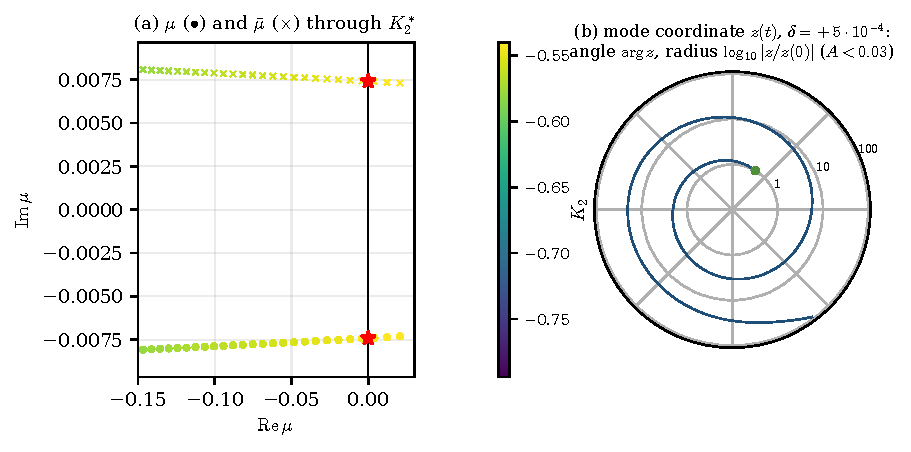
\includegraphics[width=\textwidth]{figures/fig_hopf_orbit.pdf}
\caption{The transverse Hopf point of Theorem~\ref{V3P3:thm:hopf}(a) on $Y_{168}$,
$(K_1,\alpha,\Phi)=(1,0.55,-1.40)$. (a) Along the branch of cluster equilibria, the leading eigenvalue
$\mu$ of the block $M(\lambda)$, $\lambda=2\sqrt2\,e^{-i\varphi}$ (dots), and its conjugate partner
$\bar\mu$ in $M(\bar\lambda)$ (crosses), coloured by $K_2\in[K_2^{*}-0.25,K_2^{*}+0.004]$; they cross the
imaginary axis at $\pm i\Omega_H$, $\Omega_H=0.0074144$ (stars), with speed
$d\operatorname{Re}\mu/dK_2=5.0116$, each with multiplicity $21$. (b) The full $168$-oscillator
network at $K_2=K_2^{*}+5\cdot10^{-4}$, started at amplitude $10^{-4}$ in the $42$-dimensional critical
space: the critical-mode coordinate $z(t)$ in log-polar form (angle $\arg z$, radius
$\log_{10}|z/z(0)|$), shown while the rms deviation $A<0.03$. It turns at the rate $\Omega_H$ and grows at
the linear rate $\operatorname{Re}\mu$ at first, then faster (Remark~\ref{V3P3:rem:hopfdyn}(2)), and
leaves the neighbourhood without settling on a cycle; the trajectory ends in a frequency-locked state.
Drawn by \texttt{code/make\_figures.py}.}
\label{V3P3:fig:hopf}
\end{figure}

\begin{remark}[Numerical: what happens beyond the crossing]\label{V3P3:rem:hopfdyn}
Full-network simulations (RK4, $dt=0.25$) at the point of Theorem~\ref{V3P3:thm:hopf}(a), with
$\delta=K_2-K_2^{*}$:
\begin{enumerate}
\item[(1)] \emph{Linear regime.} For $\delta=+0.0005$ the linearization gives
$\mu=0.00252+0.00740i$. Started at amplitude $10^{-4}$ in the centre space, the rms deviation $A$
grows at rate $0.00255$ and the critical-mode coordinate turns at rate $0.00743$ while
$A\in[2\cdot10^{-4},10^{-3}]$: the instability is the predicted oscillatory one
(Figure~\ref{V3P3:fig:hopf}).
\item[(2)] \emph{No saturation.} The growth then accelerates, to rates $0.0103$ for
$A\in[3\cdot10^{-3},10^{-2}]$ and $0.087$ for $A\in[10^{-2},3\cdot10^{-2}]$: the nonlinearity is
destabilizing, and there is no small-amplitude cycle to land on. The trajectory ends at a state that
is frequency-locked (spread of $\dot\theta_j$ below $2\cdot10^{-13}$) and stationary in the rotating
frame (shape change $4\cdot10^{-16}$), with $A=0.442$ and $r=(0.9994,0.9965,0.8155)$: a relative
equilibrium off the cluster subspace, in which one class is partly desynchronized.
\item[(3)] \emph{All initial directions.} For $\delta=+0.001$ and $+0.002$ (exactly the $42$ Hopf
modes are unstable there), three generic perturbations in the centre space and three pure
character modes (each of the $42$ unstable characters of the deck group spans an invariant
$3$-dimensional subspace) all end in frequency-locked stationary states, with $A$ between $0.40$ and
$0.52$.
\item[(4)] \emph{Below threshold.} The equilibrium is linearly stable, but a perturbation of size
$\varepsilon$ in a fixed generic centre direction escapes to a locked state once
$\varepsilon>\varepsilon_c$, with $\varepsilon_c=0.0053$, $0.0184$, $0.0537$ at $\delta=-0.002$,
$-0.008$, $-0.032$. So $\varepsilon_c\to0$ as $\delta\to0^{-}$, as for a subcritical bifurcation; the
fitted exponent is $0.83$, not the $\frac12$ of a generic cubic normal form, so we do not claim a
normal-form classification.
\item[(5)] \emph{A nearby steady-state crossing.} At every Hopf point examined, a real eigenvalue of
the block of $e^{i\pi/3}$ crosses zero shortly after the Hopf pair: $\delta_{\mathrm{next}}=0.0035$ at
the point of Theorem~\ref{V3P3:thm:hopf}(a), and $0.0005$, $0.0020$, $0.0020$ at three representative
points of (b). This is structural rather than accidental: all blocks share the diagonal $-\sigma_t$, so
when one block reaches the axis the others are close. The transverse Hopf points of $Y_{168}$ thus
sit near a Hopf/steady-state interaction of codimension two.
\item[(6)] \emph{Survey.} At those three representative points, each run at
$\delta=\delta_{\mathrm{next}}/5$ (so that exactly the $42$ Hopf modes are unstable) from a perturbation
of size $10^{-3}$ in the centre space, the outcome is a frequency-locked stationary state in all three
cases ($A=0.27$, $0.22$, $0.32$, each with one class partly desynchronized). An earlier survey of
$12$ Hopf points at $\operatorname{Re}\mu=+0.01$ gave the same outcome in all $12$ cases, with $A$ from
$0.30$ to $1.46$ (at the largest, $r=(0.45,0.45,0.22)$) and $\Omega_H\in[0.0027,0.0076]$.
\item[(7)] \emph{Order parameters.} The critical modes lie in $W_{[\lambda]}\oplus W_{[\bar\lambda]}$,
which is orthogonal to the class indicators (they span $W_{[\kappa]}$, and $A_1$ is normal). So the
class means of the deviation vanish, and $1-r_t=\frac12\operatorname{Var}_{V_t}(\theta)+O(A^{3})$:
the oscillation is visible in $r_0,r_1,r_2$ only at second order, and the time series of the
$r_t$ show the growth (with $1-r_t\propto A^{2}$) and the final jump, not the rotation. The rotation
is seen in the critical-mode coordinate (figure \texttt{v3p3\_hopf\_dynamics.png}).
\end{enumerate}
So transverse Hopf bifurcations exist and account for about a fifth of the losses of stability of
stable cluster states on $Y_{168}$, but no stable limit cycle, chiral or otherwise, was found near
any of them: the loss of stability is hard, and the network freezes into a locked state of the kind
seen in Remark~\ref{V3P3:rem:numerics}(2). This happens even where only the Hopf modes are linearly
unstable, but the nearby steady-state crossing of (5) means that the relevant normal form is that of a
Hopf/steady-state interaction on a $42+7$-dimensional centre space, not of an isolated Hopf point.
Whether some isotropy branch of the equivariant bifurcation is supercritical is open.
\end{remark}

\begin{remark}[Corrections to the proposed programme]\label{V3P3:rem:hopfcorrections}
(1) The crossing is not a simple Hopf bifurcation: on $Y_{168}$ the pair $\pm i\Omega_H$ has
multiplicity $21$ each, forced by the deck-group symmetry (Proposition~\ref{V3P3:prop:hopfstruct}), so
``supercritical'' in the sense of a single first Lyapunov coefficient is not defined. (2) The
bifurcation point $(K_1^{*},K_2^{*},\alpha^{*},\Phi^{*})$ is a curve family, not a point: for fixed
$(\alpha,\Phi)$ there is a value $K_2^{*}$, and Theorem~\ref{V3P3:thm:hopf} gives one to $23$ digits
and the locus at $\alpha=0.55$. (3) Beyond the crossing ($\operatorname{Re}\mu>0$) the simulations do not
produce a stable chiral limit cycle; they produce frequency-locked relative equilibria off the cluster
subspace. (4) The class order parameters $r_t(t)$ see the oscillation only at second order and are
not a good detector of it. (5) The Hopf points are not isolated codimension-one events: a real
crossing in the block of $e^{i\pi/3}$ follows within $\delta_{\mathrm{next}}=0.0005$--$0.0035$.
\end{remark}


\section{Verification battery}\label{V3P3:sec:battery}

\begin{table}[ht]
\centering\scriptsize
\renewcommand{\arraystretch}{1.2}
\resizebox{\textwidth}{!}{%
\begin{tabular}{lcl}
\toprule
check & complexes & result\\
\midrule
(G) $\delta A^{\alpha}=2\pi\alpha$; type gauge shifts $a$ by $2\pi/3$; $H_1(Y_{21})=(\Z/2)^{6}$, $64$ classes & $Y_{21},Y_{24},T_6$ & exact\\
(L) triangle lemma on a $721^{2}$ grid, $200$ values of $S$ & --- & numeric $10^{-4}$\\
(V) twisted state attains $-|E|\cos\frac{2\pi\beta}3$; $30$ random descents never lower & $Y_{21},T_6$ & numeric\\
(J) $J_m=-c_m\Delta_0$, rotation at $K_2\sin\Phi$; the $Y_{21}$ example table & $Y_{21},Y_{24},T_6$ & numeric $10^{-7}$\\
(F) $\frac1n\sum\dot\theta_j=\omega+K_2\langle m_\Delta\rangle_F$ at random states & $Y_{21},Y_{168},T_6$ & numeric $10^{-12}$\\
(R) reduced cluster Jacobian symmetric ($685$ equilibria); field $=-\nabla U+\bar m\mathbf 1$ & --- & numeric\\
(B) spectrum $=\bigcup\operatorname{spec}M(\lambda)\cup\{-\sigma_t\}$ at $46$ equilibria; real on $Y_{21}$; complex on $Y_{168}$ in $6$ & $Y_{21},Y_{168}$ & numeric $10^{-5}$\\
(O) Lyapunov inequality ($2000$ points); $60$ OA runs without chimera limit; OA defect $0.013$ vs $0.36$ & --- & numeric (seeds fixed)\\
(N) $2196$ stable cluster equilibria, none with exactly one stable class; frozen end states; solitary / disordered drift & $Y_{21},Y_{168}$ & numeric (seeds fixed)\\
(E) $\chi=n$ for $q=2$; $\chi(T_6)=0$ & $Y_{21},Y_{24},Y_{168},T_6$ & exact\\
\bottomrule
\end{tabular}}
\medskip
\caption{Checks run by \texttt{code/v3p3\_verify.py}; the complexes are built by
\texttt{code/a2\_common.py}. Section~\ref{V3P3:sec:hopf} is checked by
\texttt{code/v3p3\_hopf\_search.py}.}
\label{V3P3:tab:battery}
\end{table}

\section{Scope, residue, corrections}\label{V3P3:sec:scope}

\begin{remark}[Solved, open]\label{V3P3:rem:scope}
\emph{Solved:} the classification of chiral connections; the gradient structure of the flux
sector, with its frustrated ground states and multistability; the twisted states and their
exact spectra for all parameters; the gradient structure of the cluster subspace; the block
decomposition of the Jacobian at cluster states; OA closure and non-closure; the exclusion of
gauge chimeras for identical oscillators; the frequency sum rule; the monodromy of flux
threading. \emph{Open:}
(a) whether \eqref{V3P3:eq:model} with $K_2\ne0$ has a type-selective chimera on some family
of complexes; transverse Hopf bifurcations through a block $M(\lambda)$ do occur on $Y_{168}$
(Theorem~\ref{V3P3:thm:hopf}), and what remains open is whether any branch of this
multiplicity-$21$ equivariant bifurcation is supercritical (Remark~\ref{V3P3:rem:hopfdyn});
(b) a low-dimensional closure for the triadic term, perhaps for an OA-compatible variant that
is first harmonic in $\theta_j$;
(c) the case $\Delta>0$ of Theorem~\ref{V3P3:thm:nochimera};
(d) the role of the $|H_1|$ flat twists, which break the $\Z/3$ cluster symmetry.
\end{remark}

\begin{remark}[Corrections to the proposed programme]\label{V3P3:rem:corrections}
(1) A nonzero flux does not remove static fixed points or force a limit cycle. For $K_2=0$
the model is a gradient flow for every flux (Theorem~\ref{V3P3:thm:gradient}). Its ground
states are twisted states that carry static persistent currents
(Theorem~\ref{V3P3:thm:ground}). Breaking the conjugation $C$ is not breaking
gradient-ness. (2) $\Phi_\Delta$ is not part of the gauge field. The gauge-covariant triadic
term is blind to the flux (Remark~\ref{V3P3:rem:lag}); the only non-gradient ingredient is
the triadic lag, through the chamber drive (Theorem~\ref{V3P3:thm:clustergrad}). (3) The OA
reduction closes only for $K_2=0$ (Proposition~\ref{V3P3:prop:oa}). (4) There is no Hopf
bifurcation at twisted states, anywhere in the cluster subspace, anywhere for $K_2=0$, or at
any cluster state of $Y_{21}$ (Theorems~\ref{V3P3:thm:twisted}, \ref{V3P3:thm:clustergrad},
\ref{V3P3:thm:gradient}, Corollary~\ref{V3P3:cor:Y21real}). On $Y_{168}$ transverse Hopf points
exist, but they have multiplicity $21$ and, numerically, lead to a hard loss of stability
(Section~\ref{V3P3:sec:hopf}). A supercritical Hopf route to a chimera is not established. (5) The chimera ``$r_0\approx1$, $r_1,r_2$ incoherent'' is
impossible for $K_2=0$ and identical oscillators (Theorem~\ref{V3P3:thm:nochimera}). For
$K_2\ne0$ it is unproved, and it was not seen numerically
(Remark~\ref{V3P3:rem:numerics}). (6) The geometric phase of the synchronized rotation is
$0$. The geometric content is the $\Z/3$ monodromy of flux threading
(Propositions~\ref{V3P3:prop:berry}, \ref{V3P3:prop:monodromy}). (7) $\Delta\Omega=K_2\sin
\Phi$ is local and does not involve $\chi(Y)$ (Theorem~\ref{V3P3:thm:shift},
Remark~\ref{V3P3:rem:euler}). (8) Trees fail because every connection on a tree is pure gauge
and a graph has no $2$-cells, hence no triadic term and no non-gradient dynamics
(Proposition~\ref{V3P3:prop:tree}).
\end{remark}

\section*{Acknowledgement of provenance and caveats}

Unrefereed. The classical inputs are \L{}ojasiewicz's gradient inequality \cite{Loj63} and
LaSalle's invariance principle \cite{LaSalle60}. The Ott--Antonsen ansatz \cite{OA08} is used
only through the computation in Proposition~\ref{V3P3:prop:oa}. The chimera and triadic-coupling
literature \cite{KB02,AMSW08,SK86,SA19} is cited for context and terminology only. The
numerical observations of Remark~\ref{V3P3:rem:numerics} are exploratory and fixed-seed. The
bibliographic data of \cite{Loj63,LaSalle60,OA08,AMSW08,SK86,SA19} have been checked against Crossref and
zbMATH; \cite{KB02}, which neither indexes, was checked against the reference lists of later work.

% Volume III, Chapter 4 (drafted as "Chapter 30")
\chapter{The Geodesic Edge Operator: Unitary Remainders, Ramanujan Equivalence, and Quantum Spectral Chaos}\label{chap:V3P4}
\chaptermark{The Geodesic Edge Operator}
\begin{chapterabstract}
The proposed programme concerns the geodesic edge operator $L_E$ of an $\Atilde d$ complex. It
asks for four claims. (a) After removing the Perron root $q^{d}$, the remainder $R$ has
spectral radius exactly $q^{(d-1)/2}$ in a suitable inner product, so the Riemann hypothesis
for the edge zeta function holds \emph{unconditionally}. (b) Under the $\PGL_{d+1}(\F_q)$
symmetry the degenerate spectrum has Poisson spacings $e^{-s}$. (c) An arbitrarily small
perturbation $\varepsilon V$ produces level repulsion, with a Brody crossover to GOE ($\beta=1$)
or GUE ($\beta=2$). (d) All this ``unifies'' the Ramanujan property with quantum chaos. We
prove the correct form of (a) and correct (b)--(d).

(1) \emph{Structure.} $L_E$ is $q^{2}$-biregular and block-cyclic in the $\Z/3$ tail type,
not block-tridiagonal. It satisfies four intertwining relations with the vertex operators.
The subspace $\operatorname{im}\Psi=S^{t}\C^{V}+T^{t}\C^{V}+Q\C^{V}$ is invariant, and on it
$L_E$ is a quotient of a $3n\times3n$ matrix whose characteristic polynomial is the Hecke
pencil $\det P(u)$ of Chapter~\ref{chap:V3P1}.

(2) \emph{The unitary remainder, unconditionally.} On
$W=(\operatorname{im}\Psi)^{\perp}=\ker S\cap\ker T\cap\ker Q^{t}$, $L_E^{t}$ is exactly $\sqrt
q$ times an isometry. So the compression of $L_E$ to $W$ is $\sqrt q$ times a unitary (in fact
real orthogonal) operator, for every complex satisfying (L). The mechanism is local: the
point--hyperplane incidence of $\PG(d,q)$ is a $2$-design. The same argument works on
$\Atilde d$ with $q^{(d-1)/2}$, which is the circle of the proposed programme. Every eigenvalue of
$L_E$ has $|\lambda|\ge\sqrt q$, so $L_E$ has no Betti-number factor.

(3) \emph{The Ramanujan equivalence.} $\det(I-uL_E)=\det
P(u)\det(I-u\bar L)/\bigl((1-u^{3})(1-q^{3}u^{3})\bigr)$, where $\bar L$ is the remainder. This
holds whenever no nontrivial vertex eigenvalue lies on an explicit exceptional curve, and in
particular for all Ramanujan complexes. The nontrivial spectrum of $L_E$ lies on the two
circles $|\lambda|=q$ and $|\lambda|=\sqrt q$ \emph{if and only if} $Y$ is Ramanujan. Claim (a)
is thus false as stated: $\rho(R)=q$, not $\sqrt q$. On $Y_{21}$, $54$ eigenvalues have
modulus $2$. The Riemann hypothesis is equivalent to the Ramanujan property, not
unconditional. On $Y_{21}$,
$\det(I-uL_E)=(1-64u^{3})(1-8u^{3})^{18}(1-2u^{3}+8u^{6})^{9}(1+5u^{3}+8u^{6})^{6}$; this is
checked in full numerically and exactly at eight values of $u$.

(4) \emph{Level statistics.} A spectrum with multiplicities has an atom at $s=0$, so it is not
Poisson. On $Y_{168}$ the $226$ remainder phases of one graded piece take only $16$ values,
and $93\%$ of the spacings are exactly $0$. Under a perturbation the spectrum moves
continuously, so no arbitrarily small $\varepsilon$ gives Wigner--Dyson statistics. Numerically,
for $\varepsilon\le10^{-2}$, $93\%$ of the spacings are still below a tenth of the mean.
Brody's family is phenomenological: its $b=1$ is the GOE surmise, but its $b=2$ is \emph{not}
the GUE surmise. The symmetry class is set by antiunitary symmetries: a real $V$ gives
GUE-like statistics here. Ramanujan (where the spectrum sits) and chaos (how phases
correlate) are logically independent. What links them is the decomposition
$\C^{E}=\operatorname{im}\Psi\oplus W$.
\end{chapterabstract}

\section*{Status of the results}

Every numbered statement is proved except the numerical observations in
Remark~\ref{V3P4:rem:numerics}. The classical inputs are analytic perturbation theory
\cite{Kato}, which is used only in Proposition~\ref{V3P4:prop:split}, and the definition of
Ramanujan complexes \cite{LSV05}. The equivalence of Theorem~\ref{V3P4:thm:ramanujan} is in the
spirit of Kang--Li--Wang \cite{KLW10}. We prove it here, and we do not rely on their
statement. All identities were checked by \texttt{code/v3p4\_verify.py}
(Table~\ref{V3P4:tab:battery}).

Notation follows Chapters~\ref{chap:V3P1}--\ref{chap:V3P3}. $Y$ satisfies (L) with $q\ge2$, and $\kappa=q^{2}+q+1$. $E$ is
the set of type-increasing edges $x\to y$. $S,T\colon\C^{E}\to\C^{V}$ sum over edges with a
given tail and head: $(Sf)(x)=\sum_{x\to y}f(x\to y)$ and $(Tf)(y)=\sum_{x\to y}f(x\to y)$. For
a vertex $y$, $\mathrm{In}(y)$ and $\mathrm{Out}(y)$ are the edges into and out of $y$. In
$\mathrm{Lk}(y)$ the in-neighbours are lines and the out-neighbours are points of $\PG(2,q)$,
and $x\to y\to z$ lie in a chamber iff the point $z$ is on the line $x$. $\operatorname{Inc}_y$
is the line--point incidence matrix, $J$ the all-ones matrix. $P(u)=I-uA_1+qu^{2}A_2-q^{3}u^{3}I$
and $P_a(u)=1-au+q\bar au^{2}-q^{3}u^{3}$ for a joint eigenvalue $(a,\bar a)$ of
$(A_1,A_2)$.

\section{The geodesic edge operator}\label{V3P4:sec:LE}

\begin{definition}\label{V3P4:def:LE}
$L_E\in M_E(\Z)$ has $L_E(x\to y,\,y\to z)=1$ when $x,y,z$ do \emph{not} span a chamber, and
all other entries $0$. Define $Q\colon\C^{V}\to\C^{E}$ by $(Q\varphi)(x\to y)=\sum_{z:\{x,y,z\}\in
F}\varphi(z)$.
\end{definition}

\begin{lemma}[Local form]\label{V3P4:lem:local}
$L_E=\bigoplus_yM_y$, where $M_y=J-\operatorname{Inc}_y$ maps $\C^{\mathrm{Out}(y)}\to
\C^{\mathrm{In}(y)}$. Moreover $M_y\mathbf 1=q^{2}\mathbf 1$, $\mathbf 1^{t}M_y=q^{2}\mathbf
1^{t}$, and $M_y^{t}M_y=M_yM_y^{t}=qI+(q^{2}-q)J$. So on the complements of the constants,
$M_y$ is $\sqrt q$ times an isometry.
\end{lemma}

\begin{proof}
The continuations of $x\to y$ are the $\kappa-(q+1)=q^{2}$ points of $\mathrm{Lk}(y)$ off the
line $x$. Two distinct points lie on one common line, so
$\operatorname{Inc}^{t}\operatorname{Inc}=qI+J$; dually, $\operatorname{Inc}\operatorname{Inc}^{t}=qI+J$.
Then $M^{t}M=\kappa J-2(q+1)J+qI+J$.
\end{proof}

\begin{proposition}[Perron root and grading]\label{V3P4:prop:perron}
$L_E$ has all row and column sums equal to $q^{2}$, so $\rho(L_E)=q^{2}$ with eigenvector
$\mathbf 1_E$. $L_E$ maps edges with tail type $t$ to edges with tail type $t+1$. So
$D_EL_ED_E^{-1}=\omega L_E$ for $D_E=\operatorname{diag}(\omega^{-\tau(\mathrm{tail})})$, and the
spectrum is invariant under multiplication by $\omega$. The block structure is \emph{cyclic}
of period $3$, not tridiagonal. On $\Atilde d$ it is cyclic of period $d+1$.
\end{proposition}

\begin{proposition}[Intertwining relations]\label{V3P4:prop:relations}
\[
TL_E=q^{2}S,\qquad L_ES^{t}=q^{2}T^{t},\qquad L_ET^{t}=T^{t}A_1-Q,\qquad L_EQ=qT^{t}A_2-qS^{t},
\]
and $SS^{t}=TT^{t}=\kappa I$, $ST^{t}=A_1$, $SQ=(q+1)A_2$, $TQ=(q+1)A_1$.
\end{proposition}

\begin{proof}
The first two relations are the column and row sums of the $M_y$. For the third,
$(L_ET^{t}\varphi)(x\to y)=\sum_{z\in\mathrm{Out}(y),\,z\notin x}\varphi(z)=(A_1\varphi)(y)-(Q\varphi)(x\to y)$.
For the fourth, $(L_EQ\varphi)(x\to y)=\sum_{z\notin x}\sum_{w\ni z}\varphi(w)$, with $w$
ranging over lines of $\mathrm{Lk}(y)$. The line $w=x$ contributes nothing, and each line
$w\ne x$ contains exactly $q$ points off $x$. So the sum is
$q\bigl((A_2\varphi)(y)-\varphi(x)\bigr)$. The rest are incidence counts: each edge lies in
$q+1$ chambers.
\end{proof}

Let $\Psi\colon\C^{V}\otimes\C^{3}\to\C^{E}$, $\Psi(\varphi_1,\varphi_2,\varphi_3)=S^{t}\varphi_1+T^{t}\varphi_2+Q\varphi_3$, and
\[
\widehat N=\begin{pmatrix}0&0&-qI\\ q^{2}I&A_1&qA_2\\ 0&-I&0\end{pmatrix}.
\]

\begin{theorem}[The vertex block]\label{V3P4:thm:vertex}
$L_E\Psi=\Psi\widehat N$ and $\det(I-u\widehat N)=\det P(u)$. So $\operatorname{im}\Psi$ is
$L_E$-invariant, and $\ker\Psi$ is $\widehat N$-invariant. On a joint eigenvector with
eigenvalue $a$, $\widehat N$ acts by a $3\times3$ matrix with characteristic polynomial
$\lambda^{3}-a\lambda^{2}+q\bar a\lambda-q^{3}$.
\end{theorem}

\begin{proof}
The identity is Proposition~\ref{V3P4:prop:relations} read column by column. For the
determinant, expand $\det(\lambda I-N(a))$ with
$N(a)=\begin{psmallmatrix}0&0&-q\\q^{2}&a&q\bar a\\0&-1&0\end{psmallmatrix}$ and diagonalize
$(A_1,A_2)$ jointly.
\end{proof}

\section{The unitary remainder}\label{V3P4:sec:remainder}

\begin{theorem}[Unitary remainder, unconditional]\label{V3P4:thm:unitary}
Put $W=(\operatorname{im}\Psi)^{\perp}=\ker S\cap\ker T\cap\ker Q^{t}$. Then $L_E^{t}W\subseteq
W$ and $\|L_E^{t}f\|=\sqrt q\,\|f\|$ for $f\in W$. Hence the compression $\bar L=P_WL_E|_W$
satisfies $\bar L^{*}=L_E^{t}|_W$, and $\bar L=\sqrt q\,U$ with $U$ real orthogonal. In
particular $\rho(\bar L)=\sqrt q$, every eigenvalue of $\bar L$ lies on $|\lambda|=\sqrt q$,
and $\bar L$ is diagonalizable. No assumption beyond \textup{(L)} is used.
\end{theorem}

\begin{proof}
$W$ is the orthogonal complement of an $L_E$-invariant subspace, so it is $L_E^{t}$-invariant.
$W\subseteq\ker T$ means that $f|_{\mathrm{In}(y)}\perp\mathbf 1$ for every $y$. Now
$(L_E^{t}f)|_{\mathrm{Out}(y)}=M_y^{t}f|_{\mathrm{In}(y)}$, and both families
$\{\mathrm{In}(y)\}$ and $\{\mathrm{Out}(y)\}$ partition $E$. By Lemma~\ref{V3P4:lem:local},
$\|L_E^{t}f\|^{2}=\sum_y\|M_y^{t}f|_{\mathrm{In}(y)}\|^{2}=q\|f\|^{2}$. The rest is linear
algebra: $\langle\bar Lf,g\rangle=\langle f,L_E^{t}g\rangle$ for $f,g\in W$, and $L_E$ is real.
\end{proof}

\begin{theorem}[Lower bound]\label{V3P4:thm:lower}
Every eigenvalue of $L_E$ satisfies $|\lambda|\ge\sqrt q$, with equality iff its eigenvectors
lie in $\ker S\cap\ker T$. Consequently $1-u^{3}$ does not divide $\det(I-uL_E)$, and the Betti
numbers of $Y$ do not enter $\det(I-uL_E)$. This is unlike rank one, where the Hashimoto
operator has the eigenvalues $\pm1$ with multiplicity governed by $b_1$.
\end{theorem}

\begin{proof}
Let $L_Ef=\lambda f$, and write $f|_{\mathrm{Out}(y)}=\sigma(y)\mathbf 1+g_y$ and
$f|_{\mathrm{In}(y)}=\tau(y)\mathbf 1+h_y$ with $g_y,h_y\perp\mathbf 1$. By
Lemma~\ref{V3P4:lem:local}, $\lambda\tau=q^{2}\sigma$ and $\|h_y\|=\frac{\sqrt q}{|\lambda|}\|g_y\|$. Put
$s=\kappa\sum|\sigma|^{2}$, $G=\sum\|g_y\|^{2}$ and $\ell=|\lambda|^{2}$. Computing $\|f\|^{2}$ in
both partitions gives $s+G=\frac{q^{4}}{\ell}s+\frac q\ell G$, i.e.\
$s(\ell-q^{4})=G(q-\ell)$. If $\ell<q$, then the left side is $\le0$ and the right side is
$\ge0$, so $s=G=0$ and $f=0$. If $\ell=q$, then $s=0$, i.e.\ $Sf=0$, and then $Tf=0$.
\end{proof}

\begin{remark}\label{V3P4:rem:betti}
This sharpens Remark~\ref{V3P1:rem:betti}, which placed the factor $(1-u^{3})^{\chi(Y)}$ of the
Kang--Li zeta function on the ``edge (branch)'' side. It cannot come from the edge operator
$L_E$, which has no eigenvalue of modulus $1$. It must come from the branch operator.
\end{remark}

\begin{theorem}[The $\Atilde d$ version]\label{V3P4:thm:Ad}
Let $Y$ be a finite complex all of whose vertex links are the flag complex of $\PG(d,q)$, with
type-increasing edges $E$. Let $L_E$ continue $x\to y$ to $y\to z$ when $z\not\subset x$ in
$\mathrm{Lk}(y)$. Let $\mathcal V$ be the smallest $L_E$-invariant subspace containing
$T^{t}\C^{V}$. Then $L_E$ has Perron root $q^{d}$, and $L_E^{t}$ is $q^{(d-1)/2}$ times an
isometry on $\mathcal V^{\perp}$. Every eigenvalue satisfies $|\lambda|\ge q^{(d-1)/2}$. For
$d=2$, $\mathcal V=\operatorname{im}\Psi$.
\end{theorem}

\begin{proof}
Points and hyperplanes of $\PG(d,q)$ form a symmetric $2$-design. Each point lies on
$r=\frac{q^{d}-1}{q-1}$ hyperplanes, two points on $\lambda_2=\frac{q^{d-1}-1}{q-1}$, and
$r-\lambda_2=q^{d-1}$. So $M_y=J-\operatorname{Inc}_y$ has sums $q^{d}$, and on the complements
of the constants $M_y^{t}M_y=M_yM_y^{t}=q^{d-1}I$. The proofs of
Theorems~\ref{V3P4:thm:unitary} and~\ref{V3P4:thm:lower} go through verbatim, with
$(q^{2},q)$ replaced by $(q^{d},q^{d-1})$. For $d=2$, $\operatorname{im}\Psi$ contains
$T^{t}\C^{V}$ and is invariant, and $L_ET^{t}$ and $L_EQ$ generate $Q$ and $S^{t}$.
\end{proof}

\begin{remark}\label{V3P4:rem:local}
The proposed programme attributes the remainder circle to a ``global'' $\PGL_{d+1}(\F_q)$ symmetry.
What is used is local: the double transitivity of $\PGL_{d+1}(\F_q)$ on points of the link
makes the incidence matrix a design, and the design makes the remainder an exact isometry.
No global group acts on $Y$ for this.
\end{remark}

\section{Factorization and the Ramanujan equivalence}\label{V3P4:sec:ramanujan}

Call a joint eigenvalue $a$ \emph{trivial} if $a\in\{\kappa,\kappa\omega,\kappa\omega^{2}\}$.
These are simple, with eigenvectors $\mathbf 1,\omega^{\tau},\omega^{2\tau}$
(Lemma~\ref{V3P1:lem:sector}, Proposition~\ref{V3P1:prop:grading}). $Y$ is \emph{Ramanujan}
\cite{LSV05} if every nontrivial $a$ is tempered: $a=q(z_1+z_2+z_3)$ with $|z_i|=1$ and
$z_1z_2z_3=1$. Equivalently, every reciprocal root of $P_a$ has modulus $q$. In general the
Satake parameters have the shape $\{re^{i\alpha},r^{-1}e^{i\alpha},e^{-2i\alpha}\}$, because
$z\mapsto1/\bar z$ permutes them. Define the \emph{exceptional curve}
\[
\Gamma_q=\bigl\{(q+1)\lambda+q^{2}\lambda^{-2}:\ |\lambda|=\sqrt q\bigr\}.
\]
Then $a\in\Gamma_q$ iff $P_a$ has a reciprocal root of modulus $\sqrt q$, i.e.\ $r=q^{\pm1/2}$.
In particular $\Gamma_q$ contains no tempered value.

\begin{lemma}[The kernel of $\Psi$]\label{V3P4:lem:kernel}
$\ker\Psi=K_t\oplus K_n$, where $K_t$ is $6$-dimensional and lies over the trivial
eigenvalues. There $\widehat N$ has the eigenvalues $\omega^{k}$ and $q\omega^{k}$. $K_n\neq0$
only if some nontrivial $a$ lies on $\Gamma_q$.
\end{lemma}

\begin{proof}
$\Psi$ maps the trivial part $(\bigoplus_{\text{triv}}E_a)\otimes\C^{3}$ onto the span of
$S^{t}\chi$ for the three trivial characters $\chi$, because $S^{t}\chi$, $T^{t}\chi$ and $Q\chi$
are proportional. It maps the nontrivial part into the orthogonal complement of that span: for
instance, $\langle S^{t}\chi,\Psi v\rangle=\langle\chi,S\Psi v\rangle=0$, since $S\Psi v$ lies
in the nontrivial part. Hence $\ker\Psi$ splits, and $K_t$ has dimension $9-3=6$. On the image,
$L_ES^{t}\chi=q^{2}T^{t}\chi$ has eigenvalue $q^{2}\omega^{k}$, so the other two roots
$\omega^{k},q\omega^{k}$ of $P_{\kappa\omega^{k}}$ lie in $K_t$.

Now let $v=(\varphi_1,\varphi_2,\varphi)\in K_n$ with $\widehat Nv=\lambda v$. Then $\lambda\ne0$,
$\varphi_1=-\frac q\lambda\varphi$, $\varphi_2=-\lambda\varphi$, and $\Psi v=0$ reads
$(Q\varphi)(x\to y)=\frac q\lambda\varphi(x)+\lambda\varphi(y)$ on every edge. At a vertex $y$
this says $\operatorname{Inc}_y\varphi_{\mathrm{Out}}=\frac q\lambda\varphi_{\mathrm{In}}+
\lambda\varphi(y)\mathbf 1$, and on the edges out of $y$ it says
$\operatorname{Inc}_y^{t}\varphi_{\mathrm{In}}=\frac q\lambda\varphi(y)\mathbf
1+\lambda\varphi_{\mathrm{Out}}$. Applying $\operatorname{Inc}^{t}$ to the first, and using
$\operatorname{Inc}^{t}\operatorname{Inc}=qI+J$, gives
$A_1\varphi=a(\lambda)\varphi$ with $a(\lambda)=(q+1)\lambda+q^{2}\lambda^{-2}$.
Symmetrically, $A_2\varphi=(\lambda^{2}+q(q+1)\lambda^{-1})\varphi$. $A_1$ is normal, so the two
values are complex conjugate. Write $\bar\lambda=qt/\lambda$ with $t=|\lambda|^{2}/q$. Then
the conjugacy condition becomes $(t-1)\bigl[q(q+1)\lambda^{-1}-\lambda^{2}(1+t)t^{-2}\bigr]=0$.
Either $t=1$, i.e.\ $a\in\Gamma_q$; or $\lambda^{3}=q(q+1)t^{2}/(1+t)>0$, which forces
$|\lambda|\in\{1,q\}$ and $a(\lambda)$ trivial. The latter is impossible for $\varphi$ in
the nontrivial part. Since $K_n$ is $\widehat N$-invariant, it is $0$ unless it contains such
an eigenvector.
\end{proof}

\begin{theorem}[Factorization]\label{V3P4:thm:factor}
If no nontrivial $a$ lies on $\Gamma_q$ (in particular, if $Y$ is Ramanujan), then
$\dim W=|E|-3n+6=(q-1)(q+2)n+6$ and
\[
\det(I-uL_E)=\frac{\det P(u)}{(1-u^{3})(1-q^{3}u^{3})}\,\det(I-u\bar L),
\]
where all reciprocal roots of $\det(I-u\bar L)$ have modulus $\sqrt q$
(Theorem~\ref{V3P4:thm:unitary}).
\end{theorem}

\begin{proof}
With respect to $\C^{E}=\operatorname{im}\Psi\oplus W$, $L_E$ is block upper triangular with
diagonal blocks $L_E|_{\operatorname{im}\Psi}$ and $\bar L$. $L_E|_{\operatorname{im}\Psi}$ is
conjugate, via $\Psi$, to the map induced by $\widehat N$ on $\C^{3n}/\ker\Psi$. By
Lemma~\ref{V3P4:lem:kernel}, $\ker\Psi=K_t$, which carries
$\prod_k(1-\omega^{k}u)(1-q\omega^{k}u)=(1-u^{3})(1-q^{3}u^{3})$.
\end{proof}

\begin{theorem}[Riemann hypothesis $\Leftrightarrow$ Ramanujan]\label{V3P4:thm:ramanujan}
The eigenvalues of $L_E$ other than $q^{2}\omega^{k}$ all lie on the two circles
$|\lambda|=q$ and $|\lambda|=\sqrt q$ if and only if $Y$ is Ramanujan. Equivalently, the
nontrivial poles of $Z_E(u)=\det(I-uL_E)^{-1}$ lie on $|u|=q^{-1}$ or $|u|=q^{-1/2}$. The
circle $|u|=q^{-1/2}$ carries the $\dim W$ poles of the remainder unconditionally. On a
Ramanujan complex the circle $|u|=q^{-1}$ carries $3(n-3)$ poles, and its occupation is
\emph{exactly} the Ramanujan condition.
\end{theorem}

\begin{proof}
($\Leftarrow$) Theorem~\ref{V3P4:thm:factor}: the nontrivial $P_a$ have reciprocal roots
$qz_i$ with $|z_i|=1$, the trivial ones leave only $q^{2}\omega^{k}$, and $\bar L$ lives on the
$\sqrt q$-circle. ($\Rightarrow$) Suppose a nontrivial $a$ is not tempered, with $r>1$. Then
$N(a)$ has an eigenvector $v$ over $E_a$ with eigenvalue $\mu=qre^{i\alpha}$, and $|\mu|>q$. If
$\Psi v=0$, Lemma~\ref{V3P4:lem:kernel} forces $|\mu|=\sqrt q$, which is false. So $\Psi v$ is an
eigenvector of $L_E$ with $|\mu|\notin\{q,\sqrt q\}$.
\end{proof}

\begin{remark}[What the proposed programme's theorem gets right and wrong]\label{V3P4:rem:spec}
The circle $q^{(d-1)/2}$ is right, for the remainder $W$ (Theorems~\ref{V3P4:thm:unitary},
\ref{V3P4:thm:Ad}), and unconditionally so. It is wrong for ``$L_E$ minus its Perron root''.
That operator has spectral radius $q$ on every Ramanujan complex with $n>3$: $54$ eigenvalues
of modulus $2$ on $Y_{21}$, and $495$ on $Y_{168}$. Its $q$-circle is equivalent to the
Ramanujan property, which is a global arithmetic input, not a consequence of (L). The five
covers of this volume are all Ramanujan (line (F) of Table~\ref{V3P4:tab:battery}). ``In
a suitable inner product'' is not needed: the standard one works, provided one compresses to $W$
rather than restricting (W is $L_E^{t}$-invariant, not $L_E$-invariant).
\end{remark}

\section{Level statistics: what is provable}\label{V3P4:sec:stats}

For a finite spectrum $\{\theta_1,\dots,\theta_N\}$ on the circle, counted with multiplicity
and sorted, the \emph{empirical spacing measure} is $\frac1N\sum_i\delta_{s_i}$ with
$s_i=\frac{N}{2\pi}(\theta_{i+1}-\theta_i)$.

\begin{proposition}[Degenerate spectra are not Poisson]\label{V3P4:prop:atom}
If the spectrum has $k<N$ distinct values, the spacing measure has an atom of mass $(N-k)/N$ at
$s=0$. So it is not $e^{-s}\,ds$, and a sequence of such spectra with $(N-k)/N$ bounded below
cannot converge to it.
\end{proposition}

\begin{proof}
Exactly $N-k$ consecutive differences vanish. The measure $e^{-s}ds$ has no atoms.
\end{proof}

On $Y_{168}$, the remainder of one graded piece, $U^{3}$ on $W\cap\C^{E_0}$, has $N=226$
eigenphases with $k=16$ distinct values. The atom has mass $210/226=0.929$. The
``arithmetic Poisson spectrum'' of the proposed programme is really an arithmetic
\emph{degenerate} spectrum. The deck groups of our covers are abelian
($\Z/7$, $(\Z/2)^{3}$, $\Z/14$, $\Z/2\oplus\Z/14$, $(\Z/2)^{2}\oplus\Z/14$), so they force no
degeneracy through irreducible dimensions. Decomposing along the characters $\chi$ of the deck
group $A$, one expects pieces of dimension $18$ for $\chi=1$ (the remainder of $X_3$) and $12$
for $\chi\ne1$. This is consistent with $18+12(|A|-1)=4n+6$, but we have not verified it
piece by piece. The coincidences of values between pieces are observed, not explained.

\begin{proposition}[Splitting, but not immediately]\label{V3P4:prop:split}
Let $H_0$ be Hermitian with a repeated eigenvalue, and let $V$ be Hermitian with simple
spectrum. Then:
\begin{enumerate}
\item[(i)] $H_0+\varepsilon V$ has simple spectrum for all but finitely many $\varepsilon\in\R$;
\item[(ii)] an eigenvalue $E$ of $H_0$ of multiplicity $m$ splits as
$E+\varepsilon\mu_i+O(\varepsilon^{2})$, where the $\mu_i$ are the eigenvalues of
$P_EVP_E$ \cite{Kato};
\item[(iii)] for fixed $N$, as $\varepsilon\to0$ the spacing measure of $H_0+\varepsilon V$
converges weakly to that of $H_0$, which has an atom at $0$.
\end{enumerate}
So ``any $\varepsilon>0$ removes the degeneracy'' is true in the sense of (i), but ``any
$\varepsilon>0$ produces Wigner--Dyson statistics'' is false in the sense of (iii). The same holds
for the unitary family $U_0e^{i\varepsilon V}$ on compact $\varepsilon$-intervals.
\end{proposition}

\begin{proof}
(i) The discriminant of $\det(\lambda-H_0-\varepsilon V)$ is a polynomial in $\varepsilon$. It is
not identically zero, because $\varepsilon^{-1}(H_0+\varepsilon V)\to V$ has simple spectrum. (ii) is
first-order degenerate perturbation theory. (iii) Eigenvalues depend continuously on
$\varepsilon$. For the unitary family, the discriminant is real analytic in $\varepsilon$.
\end{proof}

\begin{proposition}[Brody is not Dyson]\label{V3P4:prop:brody}
Let $P_b(s)=(b+1)\alpha_bs^{b}\exp(-\alpha_bs^{b+1})$ with
$\alpha_b=\Gamma\bigl(\frac{b+2}{b+1}\bigr)^{b+1}$, normalized to unit mass and mean. Then
$P_0=e^{-s}$, and $P_1=\frac\pi2se^{-\pi s^{2}/4}$ is the GOE Wigner surmise. But
$P_2\neq\frac{32}{\pi^{2}}s^{2}e^{-4s^{2}/\pi}$, the GUE surmise: their logarithms decay like
$-s^{3}$ and $-s^{2}$ respectively. The Brody parameter is therefore not Dyson's index. The
family is an interpolation \cite{Brody73}, not a consequence of perturbation theory, and no
``crossover formula'' $P_\beta$ with $\beta=2$ for GUE follows from it.
\end{proposition}

\begin{remark}[Numerical observations]\label{V3P4:rem:numerics}
Let $U_3$ be the orthogonal $226\times226$ remainder of $Y_{168}$ above. Take
$U_\varepsilon=U_3e^{i\varepsilon V}$, with $V=(A+A^{*})/(2\sqrt N)$ and $A$ a complex (``GUE'') or
real (``GOE'') Gaussian matrix, and $12$ samples per $\varepsilon$ (seed fixed). We use the
unfolding-free ratio $\langle r\rangle$ of consecutive spacings; the reference values are
$0.386$ (Poisson), $0.531$ (GOE), $0.600$ (GUE) \cite{Atas13}.
\begin{center}
\begin{tabular}{lccccc}
\toprule
$\varepsilon$ & $10^{-3}$ & $10^{-2}$ & $10^{-1}$ & $1$ & $3$\\
\midrule
GUE-type $V$: $\langle r\rangle$ & 0.509 & 0.513 & 0.527 & 0.595 & 0.593\\
\quad spacings $<0.1\times$mean & 0.929 & 0.929 & 0.134 & 0.001 & 0.001\\
GOE-type $V$: $\langle r\rangle$ & 0.523 & 0.510 & 0.538 & 0.601 & 0.595\\
\quad spacings $<0.1\times$mean & 0.929 & 0.929 & 0.261 & 0.003 & 0.001\\
\bottomrule
\end{tabular}
\end{center}
(1) For $\varepsilon\le10^{-2}$ the spectrum is still $93\%$ clustered. The moderate
$\langle r\rangle$ there is an artefact: the ratios inside a split cluster follow
$P_EVP_E$ (Proposition~\ref{V3P4:prop:split}(ii)). (2) The crossover occurs around
$\varepsilon\sim0.1$, the scale at which the splittings reach the mean spacing $2\pi/226$.
(3) At saturation both kinds of $V$ give GUE-like values. $U_\varepsilon$ has no antiunitary
symmetry even for real $V$, since $\overline{U_\varepsilon}=U_3e^{-i\varepsilon V}$. GOE statistics
would require a time-reversal symmetry of the perturbed operator, not ``saturation''.
\end{remark}

\begin{remark}[Ramanujan and chaos]\label{V3P4:rem:unify}
The two properties are about different things. Ramanujan is a statement about \emph{where} the
nontrivial spectrum lies: the $q$-circle, Theorem~\ref{V3P4:thm:ramanujan}. Chaos is about
\emph{how} the phases on the $\sqrt q$-circle correlate. The five covers of this volume are all
Ramanujan, and their remainders are maximally degenerate. What is true is structural. The
decomposition $\C^{E}=\operatorname{im}\Psi\oplus W$ separates the two questions. On
$\operatorname{im}\Psi$ the vertex pencil lives, and there sits the Ramanujan condition. On $W$
lives an exact unitary quantum map $U$, in the sense of quantum graphs \cite{KS97}, whose
eigenphase statistics is the natural object for a Bohigas--Giannoni--Schmit type question
\cite{BGS84,JMRR99}. We do not prove any universality statement for $U$.
\end{remark}

\section{The example \texorpdfstring{$Y_{21}$}{Y21}}\label{V3P4:sec:example}

On $Y_{21}$, $|E|=147$. The joint eigenvalues are $7\omega^{k}$ (trivial) and $a=0$ with
multiplicity $18$ (Corollary~\ref{V3P3:cor:Y21real}), and $0$ is tempered ($z=(1,\omega,\omega^{2})$).
$\dim W=90$ and $\operatorname{rank}\Psi=57$. The characteristic polynomial is
\[
\det(I-uL_E)=(1-64u^{3})\,(1-8u^{3})^{18}\,(1-2u^{3}+8u^{6})^{9}\,(1+5u^{3}+8u^{6})^{6},
\]
The eigenvalues on both sides agree numerically, and the two integer polynomials agree exactly
at $u=1,2,3,-1,-2,5,7,-3$ (Bareiss determinants). Eight points do not determine a polynomial of
degree $147$, so the identity is checked, not proved. The factors $1-64u^{3}$ and
$(1-8u^{3})^{18}$ are proved by Theorem~\ref{V3P4:thm:factor}. The first
factor is the Perron orbit. The second is $P_0(u)=1-8u^{3}$, giving $54$ eigenvalues of modulus
$2$. The last two are the remainder: $\lambda^{3}\in\{1\pm i\sqrt7,\,(-5\pm i\sqrt7)/2\}$, all
of modulus $2^{3/2}$. The spectrum is therefore highly degenerate: only $4$ distinct values of
$\lambda^{3}$ on $W$. For the other covers, see Table~\ref{V3P4:tab:battery}.

% Volume III, Chapter 4, additional section: open problem (d) of Remark V3P4:rem:scope
\section{Breaking the arithmetic degeneracy: the crossover to GUE}\label{V3P4:sec:chaos}

This section takes up open problem (d) of Remark~\ref{V3P4:rem:scope}, and on the way settles
most of (b). Throughout, $Y=Y_{168}$, $q=2$, and $U_3$ denotes the compression of $U^{3}$ to
$W\cap\C^{E_0}$, the real orthogonal $N\times N$ matrix of Remark~\ref{V3P4:rem:numerics},
$N=226$. Its $16$ distinct eigenphases have multiplicities $21^{8},9^{2},7^{4},6^{2}$, the
spacing measure has the atom $210/226$ at $s=0$ (Proposition~\ref{V3P4:prop:atom}), and the mean
spacing is $2\pi/N=0.0278$. We perturb along one-parameter families
\[
U_\varepsilon=U_3\,e^{i\varepsilon V},\qquad V=V^{*},\qquad \Tr V^{2}=N,
\]
so that the eigenvalues of $V$ have root mean square $1$, and we ask three questions. At which
$\varepsilon$ does the degeneracy give way to level repulsion, and is that scale predicted by
first-order perturbation theory? Which Wigner--Dyson class appears at saturation, and what decides
it? Which perturbations respect the symmetry that produced the degeneracy, and what do they
leave behind? Every numerical statement below is produced by
\texttt{code/v3p4\_quantum\_chaos.py} (seed $2026$, numpy and scipy, about six minutes) and is
labelled as numerical; the propositions are proved.

\subsection*{Four kinds of perturbation}

Let $W_0\colon\C^{N}\to\C^{E}$ be an orthonormal basis of $W\cap\C^{E_0}$.
\begin{itemize}
\item[(G)] \emph{GUE-type:} $V=(A+A^{*})/2$, $A$ a complex Gaussian matrix, rescaled.
\item[(O)] \emph{GOE-type:} the same with $A$ real.
\item[(S)] \emph{On-site (gauge-type):} $d_e$ independent and uniform in $(-\pi,\pi)$ on the edges,
and $V=W_0^{t}\operatorname{diag}(d)W_0$. The diagonal operator $\operatorname{diag}(d)$ does not
preserve $W$, so $e^{i\varepsilon\operatorname{diag}(d)}$ is not a map of $W$; its compression
$V$ is Hermitian (real symmetric), and $e^{i\varepsilon V}$ is unitary on $W\cap\C^{E_0}$. This is
a random $U(1)$ potential on the edges, seen from the remainder.
\item[(L)] \emph{Local $0/\pm1$:} $M$ real symmetric on $\C^{E_0}$, with independent entries in
$\{-1,0,1\}$ on the $2352$ pairs of type-$0$ edges that share their tail or their head, and on the
diagonal; $V=W_0^{t}MW_0$.
\end{itemize}
(S) and (L) are built from the geometry, and (L) is sparse; (G) and (O) are not. All four are
rescaled to $\Tr V^{2}=N$, so that the first-order scales of Proposition~\ref{V3P4:prop:firstorder}
are comparable.

\subsection*{The first-order scale}

\begin{proposition}[First-order splitting of a unitary family]\label{V3P4:prop:firstorder}
Let $U_0$ be unitary, $V$ Hermitian, and $U_\varepsilon=U_0e^{i\varepsilon V}$. Let $e^{i\theta}$ be
an eigenvalue of $U_0$ of multiplicity $m$, with orthogonal eigenprojection $P$, and let
$\mu_1\le\dots\le\mu_m$ be the eigenvalues of $PVP$ on $\operatorname{ran}P$. Then for small
$\varepsilon$ the $m$ eigenvalues of $U_\varepsilon$ near $e^{i\theta}$ have the phases
\[
\theta+\varepsilon\mu_j+o(\varepsilon),\qquad j=1,\dots,m .
\]
In particular the $m-1$ spacings inside the cluster are $\varepsilon(\mu_{j+1}-\mu_j)+o(\varepsilon)$.
\end{proposition}

\begin{proof}
$U_\varepsilon=U_0+\varepsilon\,iU_0V+O(\varepsilon^{2})$ is analytic in $\varepsilon$, and
$e^{i\theta}$ is a semisimple eigenvalue of $U_0$, because $U_0$ is normal. By the reduction
process of analytic perturbation theory \cite{Kato}, the eigenvalues of $U_\varepsilon$ in the
$e^{i\theta}$-group are $e^{i\theta}+\varepsilon\nu_j+o(\varepsilon)$, where the $\nu_j$ are the
eigenvalues of $P(iU_0V)P=ie^{i\theta}PVP$ on $\operatorname{ran}P$; so $\nu_j=ie^{i\theta}\mu_j$,
and $e^{i\theta}(1+i\varepsilon\mu_j)+o(\varepsilon)=e^{i(\theta+\varepsilon\mu_j)}+o(\varepsilon)$.
Since the eigenvalues of $U_\varepsilon$ lie on the unit circle, their phases are
$\theta+\varepsilon\mu_j+o(\varepsilon)$.
\end{proof}

Write $\delta\mu$ for the collection of the within-cluster first-order gaps $\mu_{j+1}-\mu_j$ over
the $16$ clusters ($210$ gaps), and let $f(\varepsilon)$ be the fraction of spacings of
$U_\varepsilon$ below one tenth of the mean. Proposition~\ref{V3P4:prop:firstorder} gives two
predictions. First, $f(\varepsilon)=f_1(\varepsilon)+o(1)$ with
$f_1(\varepsilon)=N^{-1}\#\{\delta\mu:\ \varepsilon\,\delta\mu<0.2\pi/N\}$, because the spacings
between distinct clusters stay above $1.6$ mean spacings; let $\varepsilon_{1/2}$ be the solution
of $f_1(\varepsilon_{1/2})=\tfrac12$. Second, the first-order splittings reach the mean spacing at
\[
\varepsilon_1=\frac{2\pi/N}{\overline{\delta\mu}}.
\]
For (G) the matrix $PVP$ on an $m$-dimensional eigenspace is an $m\times m$ GUE matrix with entries
of variance $1/N$, so its eigenvalues fill a semicircle of radius $2\sqrt{m/N}$ and
$\overline{\delta\mu}\approx4\sqrt{m/N}/(m-1)$; for $m=21$ this is $0.061$, and
\[
\varepsilon_1\approx\frac{\pi(m-1)}{2\sqrt{mN}}=0.46 .
\]
This is sixteen times the ``naive'' scale $2\pi/N=0.028$ of a splitting of order $\varepsilon$:
inside a $21$-fold cluster the first-order spread $4\sqrt{m/N}\approx1.2$ is divided among $20$
gaps. The naive scale happens to agree with $\varepsilon_{1/2}\approx0.1\,\varepsilon_1$ within a
factor of two, but for the wrong reason.

\begin{remark}[Numerical: the crossover window]\label{V3P4:rem:crossover}
Table~\ref{V3P4:tab:cross} reports $\langle r\rangle$ (the ratio statistic of
Remark~\ref{V3P4:rem:numerics}; Poisson $0.3863$, GOE $0.5307$, GUE $0.5996$ \cite{Atas13}) and
$f(\varepsilon)$ on a grid of $26$ values $\varepsilon=10^{-4},\dots,10$ (ratio $10^{0.2}$),
averaged over $20$ samples of $V$, for the four families (G), (O), (S), (L), for the time-reversal
symmetric family (T) of Proposition~\ref{V3P4:prop:symfam} and for the deck-equivariant family
(B) of Proposition~\ref{V3P4:prop:equiv}. The observed $\varepsilon_{1/2}$ is the log-linear
crossing of $f$ through $\tfrac12$; $\varepsilon_{\mathrm{sat}}$ is the first grid value at
which $\langle r\rangle$ comes within $0.01$ of its saturation value (the mean over
$\varepsilon\ge2$; the sampling error of one grid value is about $0.004$). The findings are:
\begin{itemize}
\item[(1)] For $\varepsilon\le10^{-2}$ the spectrum is still $93\%$ clustered, for every family.
\item[(2)] The first-order prediction $\varepsilon_{1/2}$ of Proposition~\ref{V3P4:prop:firstorder},
computed from the same samples of $V$, agrees with the observed value to within $10\%$ in all six
families ($0.047$--$0.050$ against $0.048$--$0.051$), far inside the factor $3$ one might have
asked for. The scale is the same for all four non-symmetric families, including the sparse
geometric ones, because the normalization $\Tr V^{2}=N$ fixes $\overline{\delta\mu}$ to
$0.059$--$0.062$.
\item[(3)] Saturation of $\langle r\rangle$ needs splittings of a few mean spacings:
$\varepsilon_{\mathrm{sat}}/\varepsilon_1$ lies between $1.5$ and $3.5$ (the grid resolves a
factor $10^{0.2}$). The crossover window therefore spans more than a decade, from
$\varepsilon_{1/2}\approx0.05$, where the clusters have opened, to
$\varepsilon_{\mathrm{sat}}\approx1$, where the correlations between former clusters are those of
the Wigner--Dyson ensemble. At $\varepsilon=0.1$ only $13\%$ of the spacings are small, but
$\langle r\rangle=0.537$ is still far from $0.60$.
\item[(4)] At saturation all four non-symmetric families give the GUE value, $0.599$--$0.602$,
the symmetric family gives the GOE value $0.532$, and the deck-equivariant family gives the Poisson
value $0.385$.
\end{itemize}
\end{remark}

\begin{table}[ht]
\centering\small
\renewcommand{\arraystretch}{1.15}
\begin{tabular}{lcccccccc}
\toprule
family & $\varepsilon_{1/2}$ obs. & $\varepsilon_{1/2}$ 1st order & $\overline{\delta\mu}$ &
$\varepsilon_1$ & $\varepsilon_{\mathrm{sat}}$ & $\varepsilon_{\mathrm{sat}}/\varepsilon_1$ &
$\langle r\rangle_{\mathrm{sat}}$ & class\\
\midrule
(G) GUE-type       & 0.0485 & 0.0470 & 0.0615 & 0.452 & 1.00 & 2.21 & 0.599 & GUE\\
(O) GOE-type       & 0.0482 & 0.0473 & 0.0620 & 0.449 & 1.58 & 3.53 & 0.599 & GUE\\
(S) on-site        & 0.0507 & 0.0498 & 0.0585 & 0.475 & 1.00 & 2.10 & 0.600 & GUE\\
(L) local $0/\pm1$ & 0.0488 & 0.0481 & 0.0608 & 0.458 & 1.58 & 3.46 & 0.602 & GUE\\
(T) symmetric, real $V$ & 0.0488 & 0.0476 & 0.0631 & 0.441 & 1.00 & 2.27 & 0.532 & GOE\\
(B) deck-equivariant & 0.0343 & 0.0314 & 0.1403 & 0.198 & 0.10 & 0.50 & 0.385 & Poisson\\
\bottomrule
\end{tabular}
\medskip
\caption{Crossover scales (numerical; $N=226$, $20$ samples per $\varepsilon$, $\Tr V^{2}=N$).
The first-order columns are computed from the eigenvalues of $PVP$ on the $16$ eigenspaces of
$U_3$ (for (T), of $S_0$); the reference scale $2\pi/N$ is $0.0278$.}
\label{V3P4:tab:cross}
\end{table}

\subsection*{Which class, and why}

\begin{proposition}[No antiunitary time reversal for generic $V$]\label{V3P4:prop:noT}
Let $U_0$ be unitary and $V$ Hermitian, and $U_\varepsilon=U_0e^{i\varepsilon V}$.
\begin{enumerate}
\item[(i)] An antiunitary $T$ satisfies $TU_\varepsilon T^{-1}=U_\varepsilon^{-1}$ for all real
$\varepsilon$ if and only if $TU_0T^{-1}=U_0^{-1}$ and $TVT^{-1}=U_0VU_0^{-1}$.
\item[(ii)] If such a $T$ exists, then for all integers $b,c$
\[
\kappa_{b,c}(V):=\Tr\bigl(VU_0^{b}VU_0^{c}V\bigr)-\Tr\bigl(VU_0^{c}VU_0^{b}V\bigr)=0 .
\]
\item[(iii)] $\kappa_{b,c}$ is a cubic polynomial in the entries of $V$. Hence if
$\kappa_{b,c}(V_0)\ne0$ for one Hermitian (resp.\ real symmetric) $V_0$, then no such $T$ exists
for $V$ outside a proper algebraic subset of the Hermitian (resp.\ real symmetric) matrices, which
has Lebesgue measure zero.
\item[(iv)] For $U_0=U_3$: numerically $|\kappa_{1,2}(V_0)|=0.38$ for a sample of the real
symmetric family (O). So for generic real or complex $V$ the family $U_3e^{i\varepsilon V}$ has no
antiunitary time reversal, and the real structure of $U_3$ does not help: complex conjugation
$K$ commutes with $U_3$ instead of inverting it, and $KU_\varepsilon K=U_3e^{-i\varepsilon\bar V}$
is $U_{-\varepsilon}$ for real $V$, not a symmetry of $U_\varepsilon$.
\end{enumerate}
\end{proposition}

\begin{proof}
(i) If the two relations hold, then
$Te^{i\varepsilon V}T^{-1}=e^{-i\varepsilon TVT^{-1}}=U_0e^{-i\varepsilon V}U_0^{-1}$, so
$TU_\varepsilon T^{-1}=U_0^{-1}U_0e^{-i\varepsilon V}U_0^{-1}=U_\varepsilon^{-1}$. Conversely,
$\varepsilon=0$ gives the first relation. $T$ is real-linear and continuous, so it commutes with
$d/d\varepsilon$; differentiating at $\varepsilon=0$ gives
$T(iU_0V)T^{-1}=-iU_0^{-1}TVT^{-1}$ on the left and
$\frac{d}{d\varepsilon}e^{-i\varepsilon V}U_0^{-1}|_{0}=-iVU_0^{-1}$ on the right, whence
$U_0^{-1}TVT^{-1}=VU_0^{-1}$.

(ii) For antiunitary $T$ and any $A$, $\Tr(TAT^{-1})=\overline{\Tr A}$: in an orthonormal
basis $T=ZK$ with $Z$ unitary, and $TAT^{-1}=Z\bar AZ^{*}$. Apply this to
$A=VU_0^{b}VU_0^{c}V$. By (i),
$TAT^{-1}=(U_0VU_0^{-1})U_0^{-b}(U_0VU_0^{-1})U_0^{-c}(U_0VU_0^{-1})=U_0VU_0^{-b}VU_0^{-c}VU_0^{-1}$,
whose trace is $\Tr(VU_0^{-b}VU_0^{-c}V)$. On the other hand
$\overline{\Tr A}=\Tr A^{*}=\Tr(VU_0^{-c}VU_0^{-b}V)$. Equating and replacing $(b,c)$ by
$(-b,-c)$ gives $\kappa_{b,c}(V)=0$.

(iii) is clear, and (iv) is the numerical certificate; the check also confirms
$\kappa_{1,2}=0$ to machine precision for the two symmetric constructions of
Proposition~\ref{V3P4:prop:symfam}, as (ii) requires.
\end{proof}

So the GUE value in Remark~\ref{V3P4:rem:numerics} and in Table~\ref{V3P4:tab:cross} is not a
property of the perturbations: it is forced by the absence of an antiunitary symmetry compatible
with the perturbation. The converse is a construction. $U_3$ is far from symmetric
($\max|U_3-U_3^{t}|=0.51$), and it cannot be made symmetric without changing it: a real orthogonal
symmetric matrix is an involution. But $U_3$ has symmetric unitary partners with the same
spectrum.

\begin{proposition}[Time-reversal symmetric families with the spectrum of $U_3$]\label{V3P4:prop:symfam}
Let $U_3=ORO^{t}$ be a real Schur form, $O$ real orthogonal and $R$ block diagonal with $2\times2$
rotation blocks $\begin{psmallmatrix}a&b\\-b&a\end{psmallmatrix}$ ($U_3$ is normal and has no
real eigenvalue). Let $\Lambda$ be the diagonal matrix with the entries $a\pm ib$ in the place of
each block, and $D$ the diagonal matrix with the entries $1,-1$ in the place of each block.
\begin{enumerate}
\item[(a)] $S_0=O\Lambda O^{t}$ is a symmetric unitary matrix with the spectrum of $U_3$. For
real symmetric $V$ the family $U'_\varepsilon=e^{i\varepsilon V/2}S_0e^{i\varepsilon V/2}$ consists
of symmetric unitaries, has the time reversal $K$ ($KU'_\varepsilon K=U'^{-1}_\varepsilon$), and is
unitarily equivalent to $S_0e^{i\varepsilon V}$.
\item[(b)] $Z=ODO^{t}$ is a real symmetric involution with $ZU_3Z=U_3^{-1}$, so $T=ZK$ is an
antiunitary involution with $TU_3T^{-1}=U_3^{-1}$. For a real symmetric $V$ the family
$U_3e^{i\varepsilon V}$ has the time reversal $T$ if and only if $V=OMO^{t}$ with $M=YMY$, where
$Y=DR$ is a real symmetric involution; these are the matrices $O(A+YAY)O^{t}$, $A$ real symmetric.
\end{enumerate}
\end{proposition}

\begin{proof}
(a) $S_0$ is unitary and symmetric since $O$ is real and $\Lambda$ is diagonal unitary, and
$S_0=O\Lambda O^{-1}$ has the eigenvalues of $\Lambda$, which are those of $R$. For $V^{t}=V$,
$(e^{i\varepsilon V/2}S_0e^{i\varepsilon V/2})^{t}=e^{i\varepsilon V/2}S_0e^{i\varepsilon V/2}$. A
symmetric unitary $U'$ satisfies $KU'K=\bar U'=(U'^{*})^{t}=(U'^{-1})^{t}=U'^{-1}$. Finally
$e^{-i\varepsilon V/2}U'_\varepsilon e^{i\varepsilon V/2}=S_0e^{i\varepsilon V}$.

(b) A reflection conjugates a rotation to its inverse, so $DRD=R^{t}$ blockwise, and
$ZU_3Z=ODRDO^{t}=OR^{t}O^{t}=U_3^{t}=U_3^{-1}$; $Z$ is real symmetric with $Z^{2}=1$, so
$T^{2}=Z\bar Z=1$. By Proposition~\ref{V3P4:prop:noT}(i) the family has the time reversal $T$ iff
$Z\bar VZ=U_3VU_3^{-1}$. For real $V=OMO^{t}$ this reads $DMD=RMR^{t}$, i.e.\ $M=DRMR^{t}D$. From
$DRD=R^{t}$ one gets $R^{t}D=DR$, so $Y=DR$ is symmetric and $Y^{2}=DRDR=R^{t}R=1$, and the
condition is $M=YMY$. The map $A\mapsto(A+YAY)/2$ is the orthogonal projection onto this
subspace.
\end{proof}

\begin{remark}[Numerical: symmetric families are GOE]\label{V3P4:rem:sym}
Both constructions were run with real symmetric Gaussian $V$ (rescaled), the time-reversal
relations were verified to $10^{-10}$, and at saturation ($\varepsilon=3$, $40$ samples):
$\langle r\rangle=0.534$ for (a) and $0.528$ for (b), against the COE/GOE value $0.531$ and a
Haar-COE reference of $0.532$ at $N=226$. The non-symmetric families give $0.600$--$0.604$, the
Haar-CUE reference $0.602$. Note that (a) and (b) have the \emph{same} unperturbed spectrum as
(G)--(L); what differs is the position of the real structure relative to the unperturbed
operator: $K$ inverts $S_0$ but commutes with $U_3$. The reality of $U_3$, which comes from the
integrality of $L_E$, is a symmetry of the type ``spectrum closed under conjugation'', not a time
reversal; Haar-random real orthogonal matrices have GUE bulk statistics (the Weyl density of
$O(N)$ is a $\beta=2$ ensemble in $\cos\theta$), and numerically their eigenphases in $(0,\pi)$
give $\langle r\rangle=0.600$ at $N=226$. Dyson's classification applies to the pair
(operator, antiunitary symmetry), never to the operator alone.
\end{remark}

\subsection*{The saturated spacing distribution, and Brody once more}

\begin{remark}[Numerical: unfolded spacings at saturation]\label{V3P4:rem:brodyfit}
On the circle the density of eigenphases is uniform, so unfolding is the rescaling
$s_i=\frac N{2\pi}(\theta_{i+1}-\theta_i)$, which has mean exactly $1$ in every sample. For
$\varepsilon=3$ and $40$ samples ($9040$ spacings per family) Table~\ref{V3P4:tab:sat} gives the
maximum-likelihood Brody parameter $b$ of Proposition~\ref{V3P4:prop:brody}, the Kolmogorov
distance $\sup_s|F_{\mathrm{emp}}-F|$ to the Poisson, GOE and GUE surmises and to the Brody
curves with $b=2$ and with the fitted $b$, and the Kullback--Leibler divergence
$\sum_ip_i\log(p_i/q_i)$ on bins of width $0.1$. Three Haar ensembles at $N=226$ calibrate the
finite-$N$ and finite-sample effects.
\begin{itemize}
\item[(1)] For the four non-symmetric families the empirical distribution is the GUE surmise to
within the sampling resolution: Kolmogorov distance $0.006$--$0.009$, the same as for Haar CUE
($0.007$), while the distance to the Brody $b=2$ curve is $0.044$--$0.050$, which is the exact
distance $\sup|F_{P_2}-F_{\mathrm{GUE}}|=0.043$ between the two curves. The Kullback--Leibler
divergence to GUE is $0.001$--$0.002$ against $0.044$--$0.050$ to GOE.
\item[(2)] The fitted Brody parameter of a GUE spectrum is $b=1.5\pm0.05$, both here and for Haar
CUE. This is Proposition~\ref{V3P4:prop:brody} seen from the data: $\log P_b(s)$ decays like
$-\alpha_bs^{b+1}$, i.e.\ like $-s^{3}$ for $b=2$, whereas the GUE surmise decays like
$-4s^{2}/\pi$; the likelihood balances the small-$s$ behaviour $s^{2}$ (which wants $b=2$) against
the Gaussian tail (which wants $b=1$) and settles in between. A fitted $b\approx2$ would be
evidence \emph{against} GUE, not for it. For the symmetric families $b=0.93$--$0.95$, as for Haar
COE ($0.94$), and the Kolmogorov distance to the GOE surmise is $0.008$--$0.014$.
\item[(3)] For the deck-equivariant family (B) the fitted $b$ is $0.02$ and the Kolmogorov
distance to the Poisson law is $0.013$: a superposition of $56$ independent spectra of sizes $4$
and $6$ is Poisson to this resolution.
\end{itemize}
\end{remark}

\begin{table}[ht]
\centering\small
\renewcommand{\arraystretch}{1.15}
\begin{tabular}{lcccccccc}
\toprule
 & $\langle r\rangle$ & $b$ & $d_{\mathrm{Poi}}$ & $d_{\mathrm{GOE}}$ & $d_{\mathrm{GUE}}$ &
$d_{P_2}$ & $d_{P_b}$ & $\mathrm{KL}_{\mathrm{GOE}}/\mathrm{KL}_{\mathrm{GUE}}$\\
\midrule
(G) GUE-type        & 0.603 & 1.51 & 0.283 & 0.070 & 0.006 & 0.048 & 0.015 & 0.047 / 0.001\\
(O) GOE-type        & 0.602 & 1.51 & 0.284 & 0.071 & 0.009 & 0.049 & 0.017 & 0.049 / 0.002\\
(S) on-site         & 0.600 & 1.48 & 0.280 & 0.069 & 0.007 & 0.050 & 0.017 & 0.044 / 0.002\\
(L) local $0/\pm1$  & 0.604 & 1.54 & 0.286 & 0.073 & 0.006 & 0.044 & 0.016 & 0.050 / 0.002\\
(T$_a$) symmetric, $S_0$ & 0.534 & 0.95 & 0.211 & 0.008 & 0.076 & 0.111 & 0.006 & 0.002 / 0.078\\
(T$_b$) $T$-real $V$ & 0.528 & 0.93 & 0.209 & 0.014 & 0.080 & 0.118 & 0.007 & 0.003 / 0.083\\
(B) deck-equivariant & 0.386 & 0.02 & 0.013 & 0.207 & 0.271 & 0.303 & 0.006 & 0.565 / 1.251\\
(P) pull-back on-site & 0.359 & 0.01 & 0.071 & 0.247 & 0.311 & 0.337 & 0.071 & 0.852 / 1.731\\
\midrule
Haar CUE            & 0.602 & 1.52 & 0.283 & 0.073 & 0.007 & 0.043 & 0.016 & 0.049 / 0.002\\
Haar COE            & 0.532 & 0.94 & 0.211 & 0.014 & 0.078 & 0.115 & 0.008 & 0.003 / 0.081\\
Haar $O(N)$, $(0,\pi)$ & 0.600 & 1.52 & 0.284 & 0.070 & 0.008 & 0.043 & 0.018 & 0.049 / 0.004\\
\bottomrule
\end{tabular}
\medskip
\caption{Saturated regime, $\varepsilon=3$, $40$ samples, $9040$ unfolded spacings per row
(numerical). $b$ is the maximum-likelihood Brody parameter, $d_{F}$ the Kolmogorov distance of
the empirical distribution to $F$, and $P_2,P_b$ the Brody curves with $b=2$ and with the fitted
$b$. (T$_a$) is $e^{i\varepsilon V/2}S_0e^{i\varepsilon V/2}$ and (T$_b$) is $U_3e^{i\varepsilon V}$ with
$V=O(A+YAY)O^{t}$ (Proposition~\ref{V3P4:prop:symfam}); for Haar $O(N)$ the eigenphases in $(0,\pi)$
are used.}
\label{V3P4:tab:sat}
\end{table}

\subsection*{The deck group, its blocks, and what explains the coincidences}

The remaining question is what the degeneracy of $U_3$ is made of, and which perturbations
respect it. $Y_{168}\to X_3$ is the voltage cover of \texttt{a2\_common} with group
$A=(\Z/2)^{3}\times\Z/7$: its vertices are the pairs $(a,s)$, $a\in A$, $s\in\Z/3$ the type, and
the edge with label $x\in\Z/7$ out of $(a,s)$ ends at $(a+\theta(s,x),s+1)$, where
$\theta\colon\{0,1,2\}\times\Z/7\to A$ is the voltage assignment.

\begin{proposition}[Deck equivariance and the character blocks]\label{V3P4:prop:deck}
$A$ acts on $Y_{168}$ by $g\cdot(a,s)=(a+g,s)$, and this action is by type-preserving simplicial
automorphisms. Consequently the induced permutations $P_g$ of $E$ commute with $L_E$, $S$, $T$,
$Q$, preserve $W$ and each graded piece $W\cap\C^{E_t}$, and their compressions $D_g$ to
$W\cap\C^{E_0}$ are orthogonal and commute with $U_3$. Hence
\[
W\cap\C^{E_0}=\bigoplus_{\chi\in\widehat A}W_\chi,\qquad U_3W_\chi\subseteq W_\chi ,
\]
over the $56$ characters of $A$. Numerically, $\dim W_\chi=6$ for $\chi=1$ (the type-$0$ remainder of
$X_3$) and $4$ for $\chi\ne1$, so $6+55\cdot4=226$; this is the type-$0$ third of the count
$18+12\cdot55=678$ anticipated in Section~\ref{V3P4:sec:stats}.
\end{proposition}

\begin{proof}
Translation by $g$ commutes with the step maps $(a,s)\mapsto(a+\theta(s,x),s+1)$, so it maps the
edge with label $x$ out of $(a,s)$ to the edge with the same label out of $(a+g,s)$, and the
chambers, which are the closed label paths $(x,y,z)$ of the triangle presentation, to chambers.
Types are preserved by definition. $L_E,S,T,Q$ are defined from edges, types and chambers alone,
so they commute with $P_g$; then $W=\ker S\cap\ker T\cap\ker Q^{t}$ and the graded pieces are
invariant, and the compression of $(L_E^{t})^{3}$ commutes with that of $P_g$. $A$ is abelian, so
$\C^{E_0}$ is the direct sum of the isotypic subspaces of its characters, each $D_g$-invariant
subspace splits accordingly, and $U_3$ preserves the pieces since it commutes with all $D_g$. The
dimensions are counted by the script (the $\chi$-isotypic part of $\C^{E_0}$ is $7$-dimensional,
since $A$ acts freely on $E_0$ with $7$ orbits, and $W_\chi$ is cut out by the three
$\chi$-twisted constraints $S,T,Q^{t}$).
\end{proof}

\begin{remark}[Numerical: inside and across the blocks]\label{V3P4:rem:blocks}
The block spectra are as follows (phases of $U_3$ in degrees; $\mu=2^{3/2}\lambda$ is the
corresponding eigenvalue of $(L_E^{t})^{3}$).
\begin{center}
\begin{tabular}{llll}
\toprule
order of $\chi$ & blocks & phases & block polynomial in $\mu$\\
\midrule
$1$ & $1$ & $152.11^{3},\,207.89^{3}$ & $(\mu^{2}+5\mu+8)^{3}$\\
$7$, $\chi(1)\in\{\zeta,\zeta^{2},\zeta^{4}\}$ & $3$ & $69.30^{3},\,152.11$ & $(\mu-2\pi)^{3}(\mu-\bar\pi^{3})$\\
$7$, $\chi(1)\in\{\zeta^{3},\zeta^{5},\zeta^{6}\}$ & $3$ & $207.89,\,290.71^{3}$ & $(\mu-2\bar\pi)^{3}(\mu-\pi^{3})$\\
$2$ & $7$ & $66.72,\,113.28,\,246.72,\,293.28$ & $\mu^{4}+11\mu^{2}+64$\\
$14$, $\chi|_{\Z/7}$ a square & $21$ & $59.32,\,178.57,\,201.67,\,280.44$ & \\
$14$, $\chi|_{\Z/7}$ a non-square & $21$ & $79.56,\,158.33,\,181.43,\,300.68$ & \\
\bottomrule
\end{tabular}
\end{center}
Here $\zeta=e^{2\pi i/7}$ and $\pi=\frac{1+\sqrt{-7}}2$, the prime above $2$ in
$\Q(\sqrt{-7})$; the phases of the $\Z/7$ sector are $\pm\varphi$ and $\pm3\varphi$ with
$\varphi=\arg\pi=\arctan\sqrt7=69.295^\circ$, and the four values of $\lambda^{3}$ there are
$2^{-3/2}$ times the four elements $2\pi,2\bar\pi,\pi^{3},\bar\pi^{3}$ of norm $8$ in
$\Z[\pi]$. The $\Z/7$ sector (characters trivial on $(\Z/2)^{3}$) is the pull-back of the type-$0$
remainder of $Y_{21}$, of dimension $6+6\cdot4=30=90/3$, and the exponents $9$ and $6$ of the
polynomial of Section~\ref{V3P4:sec:example} are visible as the multiplicities $9=3\cdot3$ of
$2\pi,2\bar\pi$ and $6=3+3\cdot1$ of $\pi^{3},\bar\pi^{3}$. The block polynomials were verified
to $10^{-6}$.

(i) \emph{Within a block.} The $49$ blocks of characters of order $2$ and $14$ have simple
spectrum, with a smallest gap of $0.40$ rad, i.e.\ $14.5$ mean spacings. The $7$ blocks of the
$\Z/7$ sector are not simple: they carry triple eigenvalues. (ii) \emph{Across blocks.} Of the
$1866$ coincident pairs of eigenphases, $24$ lie inside one block and $1842$ across blocks; every
one of the $16$ values occurs in at least $3$ blocks. The $56$ block spectra form exactly the $6$
multisets of the table.
\end{remark}

The six classes are not a coincidence. The triangle presentation of \texttt{a2\_common} has the
chambers $(c,c+1,c+3)$, $c\in\Z/7$ (cyclic triples): the translates of the Singer difference set
$\{0,1,3\}$ of $\PG(2,2)$.

\begin{proposition}[Automorphisms of $X_3$ explain the cross-block coincidences]\label{V3P4:prop:aut}
\begin{enumerate}
\item[(i)] The affine maps $x\mapsto ax+b$ of $\Z/7$ with $a\in\{1,2,4\}$ preserve the chamber
list, hence act on $X_3$ as type-preserving automorphisms fixing the three vertices; they form
the Frobenius group $F_{21}=\Z/7\rtimes\Z/3$.
\item[(ii)] Every automorphism of $X_3$ lifts to $Y_{168}$, and the lift normalizes $A$; it acts
on $A$ by an automorphism $\phi$ and maps $W_\chi$ isometrically onto $W_{\chi\circ\phi^{-1}}$,
commuting with $U_3$. Blocks in one orbit of this action are isospectral.
\item[(iii)] (Numerical.) The lifts of $x\mapsto x+1$ and $x\mapsto2x$ were constructed
explicitly (vertex maps $(a,s)\mapsto(\phi(a)+c_s,s)$; the lift of $x\mapsto x+1$ acts trivially on
$\Z/7$ and by an element of order $7$ of $\GL_3(\F_2)$ on $(\Z/2)^{3}$, the lift of
$x\mapsto2x$ by multiplication by $2$ on $\Z/7$ and by an element of order $3$). Their orbits on
the $56$ characters have sizes $1,3,3,7,21,21$ and coincide with the six spectral classes. So
$1824$ of the $1842$ cross-block coincidences are between blocks in one orbit, and are explained.
\end{enumerate}
\end{proposition}

\begin{proof}
(i) Translation is obvious. Doubling maps the cyclic triple $(c,c+1,c+3)$ to $(2c,2c+2,2c+6)$,
which is the cyclic rotation $(d,d+1,d+3)$ with $d=2c+6$. The maps generate $F_{21}$, and the
chamber condition and the types are preserved, so these are automorphisms of $X_3$.
(ii) $Y_{168}$ is the cover of $X_3$ defined by the kernel of
$\pi_1(X_3)\to H_1(X_3;\Z)\to H_1(X_3;\Z)\otimes\Z/14=A$, since the voltages are a basis of the
null spaces of the relator matrix modulo $2$ and modulo $7$. This kernel is characteristic, so
every automorphism of $X_3$ lifts, and the lift normalizes the deck group and induces an
automorphism $\phi$ of $A$. A lift $\tau$ is a type-preserving automorphism of $Y_{168}$, so it
commutes with $L_E,S,T,Q$, preserves $W\cap\C^{E_0}$ and commutes with $U_3$ there; and
$\tau D_g\tau^{-1}=D_{\phi(g)}$ gives $\tau W_\chi=W_{\chi\circ\phi^{-1}}$. (iii) is checked by
the script: the lifts are found by solving $\phi(\theta(s,x))-\theta(s,\pi(x))=c_s-c_{s+1}$
over $\phi\in\GL_3(\F_2)\times(\Z/7)^{\times}$ (one solution each), the resulting edge permutations
commute with $L_E,S,T,Q$ and with $U_3$ and normalize $A$, and the orbit count is $1,3,3,7,21,21$.
\end{proof}

What is \emph{not} explained by $A$ and $\operatorname{Aut}(X_3)$ is confined to the $\Z/7$
sector: the $24$ coincidences inside a block (the triple $2\pi$ in each order-$7$ block, the
triples $\pi^{3},\bar\pi^{3}$ in the trivial block) and the $18$ coincidences between the trivial
block and the order-$7$ blocks. These are the exponents $9$ and $6$ of the $Y_{21}$ polynomial,
and the identification of the values with the norm-$8$ elements of $\Z[\pi]$, $\Q(\sqrt{-7})$
being the field of the quadratic Gauss sum of $\Z/7$, is as far as we go. This is what remains of
open problem (b) for $Y_{168}$.

\begin{proposition}[Deck-equivariant perturbations]\label{V3P4:prop:equiv}
Let $V$ be Hermitian and commute with all $D_g$, i.e.\ $V=\bigoplus_\chi V_\chi$. Then
$U_\varepsilon=U_3e^{i\varepsilon V}$ preserves every $W_\chi$, and
$\det(\lambda-U_\varepsilon)=\prod_\chi\det(\lambda-U_{\chi,\varepsilon})$. Along such a family,
eigenphases of different blocks cross: their coincidence is one real equation in $\varepsilon$,
so for generic $V$ it happens at isolated $\varepsilon$ and transversally, without repulsion.
Eigenphases of one block do not cross for generic $V$: the unitary $d\times d$ matrices with a
repeated eigenvalue form a set of real codimension $3$. Consequently the saturated statistics of
the family is that of a superposition of $56$ independent spectra of sizes $4$ and $6$, and in
particular not Wigner--Dyson.
\end{proposition}

\begin{proof}
$e^{i\varepsilon V}=\bigoplus e^{i\varepsilon V_\chi}$ and $U_3=\bigoplus U_\chi$ by
Proposition~\ref{V3P4:prop:deck}, so the blocks are preserved and the characteristic polynomial
factors. Two eigenphases from different blocks are two analytic functions of $\varepsilon$ with
independent perturbations, and their difference vanishes on a discrete set for generic $V$. For
the codimension count, a unitary $d\times d$ matrix with exactly one double eigenvalue is
$W\operatorname{diag}(\lambda_1,\lambda_1,\lambda_3,\dots,\lambda_d)W^{*}$, and the stabilizer of
the diagonal matrix is $U(2)\times U(1)^{d-2}$ of dimension $d+2$, so these matrices form a set of
dimension $(d-1)+d^{2}-(d+2)=d^{2}-3$. Levels of distinct blocks are therefore uncorrelated, and
levels within a block repel; this is a superposition.
\end{proof}

\begin{remark}[Numerical: deck-equivariant and pull-back perturbations]\label{V3P4:rem:equiv}
(B) \emph{Independent blocks.} $V=\bigoplus_\chi B_\chi H_\chi B_\chi^{*}$ with independent
GUE blocks $H_\chi$ of sizes $4$ and $6$, rescaled. The commutation with the $D_g$ and the block
invariance of $U_\varepsilon$ were verified; a generic $V$ of type (G) does not commute. At
saturation every exact coincidence is lifted (no zero spacings in $40$ samples), but
$\langle r\rangle=0.386$ (Poisson $0.3863$), $f=0.09$ (Poisson $1-e^{-0.1}=0.095$), and the
Kolmogorov distance to the Poisson law is $0.013$: the cross-block degeneracy is replaced by the
absence of cross-block repulsion, which is what Proposition~\ref{V3P4:prop:equiv} predicts.
The first-order scale is larger ($\overline{\delta\mu}=0.14$, since a $4\times4$ block has few,
wide gaps) and the crossover is correspondingly earlier ($\varepsilon_{1/2}=0.034$, again within
$10\%$ of the first-order prediction $0.031$).

(P) \emph{Pull-backs from $X_3$.} An on-site potential constant on the $21$ deck orbits of edges
(the pull-back of an on-site potential on $X_3$; $7$ free parameters on the type-$0$ edges) is
deck-equivariant, and it keeps an exact degeneracy: in every sample, at every $\varepsilon$ tested,
the three blocks of each class $\{\chi,\chi^{2},\chi^{4}\}$ of characters of order $7$ remain
isospectral, so the spectrum has $8$ triple eigenphases ($16$ zero spacings per sample, $640$ in
$40$), and $\langle r\rangle=0.359$. The lifted automorphism $x\mapsto2x$ of
Proposition~\ref{V3P4:prop:aut} maps $W_\chi$ to $W_{\chi^{2}}$ but conjugates the potential
$d$ to $d\circ(2x)^{-1}$, so it does not explain this; the entrywise moduli of the orthogonal
projections onto $W_\chi$ and $W_{\chi^{2}}$ agree to $10^{-16}$, while the obvious gauge
$\operatorname{diag}(\chi(a_e))$ does not map $W_\chi$ to $W_{\chi^{2}}$. We record the
observation without a proof.

So the ``discrete subgroup symmetry'' statement is this: the degeneracy of $U_3$ is the
$A$-block structure together with the $F_{21}$ permutation of the blocks and the arithmetic of
$\Q(\sqrt{-7})$ inside the $\Z/7$ sector. A perturbation that commutes with $A$ keeps the blocks
and produces Poisson statistics at best; the GUE statistics of Table~\ref{V3P4:tab:sat} require a
perturbation that mixes the blocks, and the GOE statistics require in addition an antiunitary
symmetry of the perturbed family, which the real structure of $U_3$ does not provide.
\end{remark}

\subsection*{The full remainder on $W$ and the window $\varepsilon\le1/\dim W$}

The question is sometimes posed for the remainder $U$ itself, on all of $W$ ($\dim W=4n+6=678$),
and for the window $0\le\varepsilon\le1/\dim W$: does $\langle r\rangle$ cross over to the GUE value
there? It does not, and the reason is a limit that can be computed exactly. Everything below is
produced by \texttt{code/v3p4\_gue\_transition.py} (seed $2027$, about $25$ minutes; data and figures
in \texttt{data/}).

Let $U_0=W^{t}L_EW/\sqrt q$ on $W$, $N=\dim W=678$. It is real orthogonal, and the grading
$J=\omega^{\mathrm{type}}$ ($\omega=e^{2\pi i/3}$) satisfies $JU_0J^{-1}=\omega^{-1}U_0$, because
$L_E$ raises the type by one. Hence $\operatorname{spec}U_0$ is invariant under rotation by
$2\pi/3$ and consists of the cube roots of $\operatorname{spec}U_3$: $48$ distinct eigenphases with
multiplicities $21^{24},9^{6},7^{12},6^{6}$, and the same atom $630/678=0.929$ at $s=0$. Every
eigenvalue is non-real, so every eigenspace $P_k$ is a complex subspace on which $P_kVP_k$ is a
complex Hermitian matrix even for real $V$. Besides (G) and (O) we use the geometric phase
perturbation (S): a random $U(1)$ potential $d_e\in(-\pi,\pi)$ on the edges, $V=W^{t}\operatorname{diag}(d)W$.
It commutes with $J$, so $U_0e^{i\varepsilon V}$ stays $\Z/3$-covariant; for all three families
$\kappa_{1,2}(V)\ne0$, so no family has an antiunitary time reversal
(Proposition~\ref{V3P4:prop:noT}).

\begin{proposition}[The first-order plateau]\label{V3P4:prop:plateau}
Let $U_0$ be unitary on $\C^{N}$ with distinct eigenvalues $e^{i\theta_k}$ of multiplicities
$m_k\ge2$ and eigenprojections $P_k$, let $V$ be Hermitian such that every $P_kVP_k$ has simple
spectrum $\mu_{k,1}<\dots<\mu_{k,m_k}$ on $\operatorname{ran}P_k$, and put
$g_{k,j}=\mu_{k,j+1}-\mu_{k,j}$. Let $\langle r\rangle(\varepsilon)$ be the mean over the $N$
consecutive pairs of spacings of $U_\varepsilon=U_0e^{i\varepsilon V}$ on the circle of
$\min(s_i,s_{i+1})/\max(s_i,s_{i+1})$. Then
\[
\lim_{\varepsilon\to0^{+}}\langle r\rangle(\varepsilon)=\langle r\rangle_1:=\frac1N\sum_k
\sum_{j=1}^{m_k-2}\frac{\min(g_{k,j},g_{k,j+1})}{\max(g_{k,j},g_{k,j+1})}
\ \le\ \frac{N-2K}{N},
\]
$K$ the number of clusters, while $\langle r\rangle(0)$ is undefined (pairs $0/0$).
\end{proposition}

\begin{proof}
By Proposition~\ref{V3P4:prop:firstorder} the eigenphases near $\theta_k$ are
$\theta_k+\varepsilon\mu_{k,j}+o(\varepsilon)$, so for small $\varepsilon>0$ they stay ordered as
the $\mu_{k,j}$, the $m_k-1$ spacings inside the cluster are $\varepsilon g_{k,j}+o(\varepsilon)$,
and the $K$ spacings between neighbouring clusters tend to the positive gaps of
$\operatorname{spec}U_0$. Among the $N$ pairs of consecutive spacings, $m_k-2$ lie inside the
$k$-th cluster, and their ratios tend to $\min(g_{k,j},g_{k,j+1})/\max(g_{k,j},g_{k,j+1})$ because
the ratio is homogeneous of degree $0$; the remaining $2K$ pairs consist of one spacing $O(\varepsilon)$
and one bounded below, so their ratio tends to $0$. Each ratio is at most $1$.
\end{proof}

So the ratio statistic does not see the size of the splitting at all, only the shape of the
first-order spectra $P_kVP_k$: it jumps at $\varepsilon=0^{+}$ to $\langle r\rangle_1$ and stays
there as long as the clusters have not met. For $Y_{168}$, $N-2K=582$, and if each $P_kVP_k$ is
a GUE-like matrix the internal ratios average about $0.59$, which predicts
$\langle r\rangle_1\approx0.858\cdot0.59\approx0.51$, between Poisson and GOE and \emph{not}
the GUE value.

\begin{figure}[t]
\centering
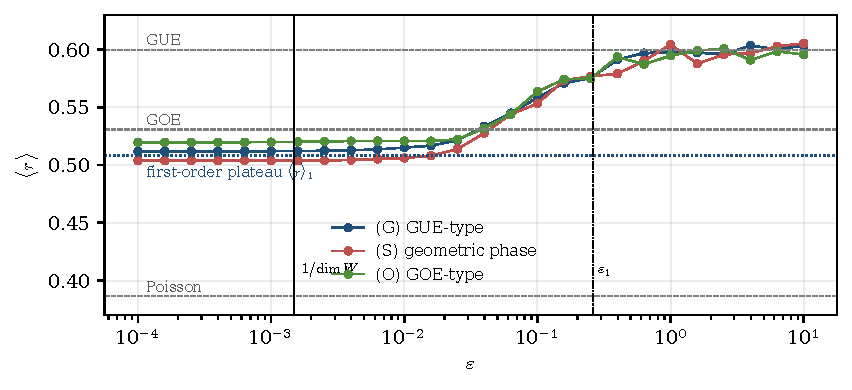
\includegraphics[width=\textwidth]{figures/fig_quantum_chaos_crossover.pdf}
\caption{The ratio statistic $\langle r\rangle$ of $U_0e^{i\varepsilon V}$ on the full space $W$ of
$Y_{168}$ ($\dim W=678$) against the perturbation strength, $\varepsilon=10^{-4},\dots,10$ ($26$ values,
$8$ samples each), for a GUE-type perturbation (G), the geometric phase perturbation (S) and a GOE-type
perturbation (O), all with $\Tr V^{2}=\dim W$. The dotted line is the first-order plateau
$\langle r\rangle_1=0.5083$ of Proposition~\ref{V3P4:prop:plateau}; the sample-to-sample scatter of the
plateau is visible below $\varepsilon\approx10^{-2}$. The solid vertical line marks the window edge
$\varepsilon=1/\dim W$, deep inside the plateau, and the dash-dotted line the first-order scale
$\varepsilon_1=0.26$ at which the mean splitting reaches the mean spacing. Saturation at the GUE value
$0.600$ occurs for $\varepsilon\gtrsim0.4$. Data of \texttt{code/v3p4\_gue\_transition.py}, drawn by
\texttt{code/make\_figures.py}.}
\label{V3P4:fig:crossover}
\end{figure}

\begin{remark}[Numerical: the window and beyond]\label{V3P4:rem:window}
\begin{enumerate}
\item[(1)] \emph{Window} $0\le\varepsilon\le1/N=1.475\cdot10^{-3}$, $21$ values, $16$ samples. For
all three families $\langle r\rangle$ is flat on the whole window and equal to the first-order
plateau computed from the same $V$:
\begin{center}\small
\begin{tabular}{lccccc}
\toprule
family & $\varepsilon=\frac1{20N}$ & $\frac1{4N}$ & $\frac1{2N}$ & $\frac1N$ & $\langle r\rangle_1$ (Prop.~\ref{V3P4:prop:plateau})\\
\midrule
(G) GUE-type & 0.5083 & 0.5084 & 0.5085 & 0.5087 & $0.5083\pm0.0030$\\
(S) geometric phase & 0.5082 & 0.5082 & 0.5083 & 0.5085 & $0.5082\pm0.0072$\\
(O) GOE-type & 0.5096 & 0.5096 & 0.5097 & 0.5099 & $0.5095\pm0.0031$\\
\bottomrule
\end{tabular}
\end{center}
At $\varepsilon=1/N$ the fraction of spacings below $0.1$ is still $0.929$, the atom itself, and the
first-order spread of a $21$-fold cluster is $0.11$ mean spacings. The real family (O) gives the
same plateau as (G) because the eigenspaces of $U_0$ are complex.
\item[(2)] \emph{Extended scan} $\varepsilon=10^{-4},\dots,10$ ($26$ values, $8$ samples;
Figure~\ref{V3P4:fig:crossover}).
$\langle r\rangle$ stays on the plateau ($0.50$--$0.52$ with $8$ samples) up to
$\varepsilon\approx10^{-2}$, rises through the GOE value near $\varepsilon\approx0.03$, and reaches
the GUE value; above $\varepsilon\approx0.4$ it fluctuates around $0.60$. The scales are
$\varepsilon_{1/2}=0.028$ (half of the spacings have opened), $\varepsilon_1=0.26$ (mean first-order
splitting $=$ mean spacing; the formula $\pi(m-1)/(2\sqrt{mN})$ with $m=21$ gives $0.263$), and
$\varepsilon_{\mathrm{sat}}=0.40$ for (G), (O) and $0.63$ for (S), i.e.\ $270$--$430$ times $1/N$;
$\langle r\rangle_{\mathrm{sat}}=0.601$, $0.600$, $0.596$.
\item[(3)] \emph{Spacing distributions} ($24$ samples, $16272$ spacings each). At $\varepsilon=1/N$
the empirical $P(s)$ is the atom plus a small continuous part; the maximum-likelihood Brody
parameter sits at the boundary $b=0$ of the family, which cannot represent an atom, and the
Kolmogorov distances to the Poisson, GOE and GUE laws are $0.91$--$0.93$. At $\varepsilon=\varepsilon_1$:
$\langle r\rangle=0.577$ and $0.580$, still $b=0$ because of the excess of small spacings. At
$\varepsilon=3$: $\langle r\rangle=0.601$ (G), $0.597$ (S), $b=1.53$ and $1.51$ (the GUE value of
the estimator, Remark~\ref{V3P4:rem:brodyfit}), Kolmogorov distance $0.005$ and $0.010$ to the GUE
surmise against $0.069$ and $0.072$ to GOE.
\end{enumerate}
So the answer to the question is negative in the window and positive outside it: on
$0<\varepsilon\le1/\dim W$ the statistic is pinned at the plateau $\langle r\rangle_1\approx0.51$
of Proposition~\ref{V3P4:prop:plateau}, and the GUE value $0.600$ is reached only for
$\varepsilon\gtrsim0.4$, where the first-order splittings exceed the mean spacing; the scale is
$\varepsilon_1\propto(m-1)/\sqrt{mN}$, not $1/N$.
\end{remark}

\begin{remark}[Scope]\label{V3P4:rem:chaosscope}
Proved: Propositions~\ref{V3P4:prop:firstorder}, \ref{V3P4:prop:noT}(i)--(iii),
\ref{V3P4:prop:symfam}, \ref{V3P4:prop:deck} except the block dimensions,
\ref{V3P4:prop:aut}(i)--(ii), \ref{V3P4:prop:equiv}, \ref{V3P4:prop:plateau}. Numerical, with the
code as the record: Tables~\ref{V3P4:tab:cross} and~\ref{V3P4:tab:sat}, Remark~\ref{V3P4:rem:window}, the block dimensions and spectra, the lifts and
their orbits, the certificate $\kappa_{1,2}(V_0)\ne0$, and the persistence of the Galois triples
under pull-back potentials. Not proved: any universality statement for the family
$U_\varepsilon$ as $n\to\infty$; the numbers here concern one complex, $Y_{168}$, and what they
establish is that on this complex the crossover scale is the first-order splitting scale, and the
symmetry class is decided by the antiunitary symmetries of the perturbed family, in the sense of
\cite{BGS84,KS97}, not by the arithmetic that produced the degeneracy.
\end{remark}


\section{Verification battery}\label{V3P4:sec:battery}

\begin{table}[ht]
\centering\scriptsize
\renewcommand{\arraystretch}{1.2}
\resizebox{\textwidth}{!}{%
\begin{tabular}{lcl}
\toprule
check & complexes & result\\
\midrule
(R) sums $q^{2}$; block-cyclic; the relations of Proposition~\ref{V3P4:prop:relations} & five covers & exact\\
(U) $W$ is $L_E^{t}$-invariant, $\|L_E^{t}f\|=\sqrt2\|f\|$; $\operatorname{rank}\Psi=3n-6$, $\dim W=4n+6$ & five covers & numeric $10^{-10}$\\
(F) $\operatorname{spec}L_E$ as in Theorem~\ref{V3P4:thm:factor}; $|\lambda|\ge\sqrt2$; Ramanujan; circle counts $(q,\sqrt q)$: & & \\
\quad $Y_{21}$ $(54,90)$, $Y_{24}$ $(63,102)$, $Y_{42}$ $(117,174)$, $Y_{84}$ $(243,342)$, $Y_{168}$ $(495,678)$ & five covers & numeric $10^{-6}$\\
(X) the $Y_{21}$ product formula at $u=1,2,3,-1,-2,5,7,-3$ & $Y_{21}$ & exact\\
(K) $\ker\Psi$ $6$-dimensional, trivial characters; $\Gamma_q$ property and disjointness from tempered $a$ ($q\le5$) & five covers & numeric\\
(D) $J-\operatorname{Inc}(\PG(d,q))$: sums $q^{d}$, $q^{d-1}$ on $\mathbf 1^{\perp}$, $(d,q)\in\{(2,2),(2,3),(3,2),(3,3),(4,2)\}$ & --- & numeric $10^{-8}$\\
(S) distinct $\lambda^{3}$ on $W$: $4,6,16,16,16$; atom $210/226$; perturbation table & $Y_{168}$ & numeric (seed 1)\\
(B) Brody $b=1$ is the GOE surmise; $b=2$ differs from GUE by $0.162$ (sup) & --- & numeric\\
\bottomrule
\end{tabular}}
\medskip
\caption{Checks run by \texttt{code/v3p4\_verify.py}. Section~\ref{V3P4:sec:chaos} is checked by
\texttt{code/v3p4\_quantum\_chaos.py} and \texttt{code/v3p4\_gue\_transition.py}.}
\label{V3P4:tab:battery}
\end{table}

\section{Scope, residue, corrections}\label{V3P4:sec:scope}

\begin{remark}[Solved, open]\label{V3P4:rem:scope}
\emph{Solved:} the local form and intertwining relations of $L_E$; the unconditional unitary
remainder, for all $d$; the lower bound $|\lambda|\ge q^{(d-1)/2}$; the factorization and the
Ramanujan equivalence for $d=2$; the exact kernel of $\Psi$; the exact polynomial for $Y_{21}$.
\emph{Open:} (a) the vertex block for $d\ge3$, which needs one operator like $Q$ for each
intermediate type; (b) an explanation of the few distinct remainder values on abelian covers;
(c) a (L)-complex with $q\ge2$ that is not Ramanujan, or a proof that none exists among
quotients of a given building; (d) any universality statement for the eigenphases of $U$ along
families.
\end{remark}

\begin{remark}[Corrections to the proposed programme]\label{V3P4:rem:corrections}
(1) The block structure of $L_E$ is cyclic in the type grading, not tridiagonal. (2) The
unconditional theorem is the unitary remainder on $W$, with $\rho=q^{(d-1)/2}$. The spectral
radius of $L_E$ away from the Perron orbit is $q$, not $q^{(d-1)/2}$, and the full
Riemann hypothesis for $\det(I-uL_E)$, in its two-circle form, is \emph{equivalent} to the
Ramanujan property (Theorem~\ref{V3P4:thm:ramanujan}). (3) Degenerate spectra have an atom at
$0$ and are not Poisson (Proposition~\ref{V3P4:prop:atom}). $\PGL_{d+1}(\F_q)$ acts on links,
not on $Y$. (4) $L_E$ is not Hermitian, so $L_E+\varepsilon V$ is not a Hamiltonian. The
natural unitary object is $U$ on $W$. A ``nonlinear'' perturbation has no spectrum; we use
linear ones. (5) Small $\varepsilon$ splits degeneracies but does not produce Wigner--Dyson
statistics (Proposition~\ref{V3P4:prop:split}); the crossover requires splittings of the order
of the mean spacing. (6) Brody's parameter is not Dyson's $\beta$: $b=2$ is not GUE
(Proposition~\ref{V3P4:prop:brody}). GOE versus GUE is decided by antiunitary symmetries
(Remark~\ref{V3P4:rem:numerics}(3)). (7) The ``unification'' is the decomposition
$\operatorname{im}\Psi\oplus W$, not an implication between Ramanujan and chaos
(Remark~\ref{V3P4:rem:unify}).
\end{remark}

\section*{Acknowledgement of provenance and caveats}

Unrefereed. The definition of Ramanujan complexes is that of \cite{LSV05}. The two-circle
characterization is in the spirit of \cite{KLW10}, and it is proved here independently. The
perturbation-theoretic and random-matrix references \cite{Kato,Brody73,Atas13,KS97,BGS84,JMRR99}
are cited for standard facts and terminology. The bibliographic data of these references
have been checked against Crossref and zbMATH.

% Volume III, Paper 5 (drafted as "Chapter 31")
\chapter{Chamber Games and Higher-Order Interactions: Pairwise Reductions, Interfaces, and Entrainment}\label{chap:V3P5}
\chaptermark{Chamber Games}
\begin{chapterabstract}
The proposed programme places a three-player public-goods game on every chamber of an $\Atwo$
complex, with strategies updated by the Fermi rule. It asks for four claims. (a) A ``topological
shielding cage'' built from the $\PG(2,q)$ flags lowers the critical synergy to
$r_c=1+2/(q+1)$. (b) This is far below the value $r_c>3$ of ``traditional regular networks'',
a ``topological catalysis'' that grows with the thickness $q$. (c) A $\Z/3$-chiral
rock--paper--scissors variant has a torus attractor and persistent oscillations in the
replicator dynamics. (d) There is a global phase diagram in $|F|/|V|$. We prove the
following.

(1) \emph{Pairwise reduction.} The public-goods payoff is linear in the strategies. On
\emph{every} $2$-complex the chamber game is therefore the additive pairwise game
$\pi_i=(\frac r3-1)D_2(i)s_i+\frac r3\sum_jw_{ij}s_j$ on the $1$-skeleton, where $w_{ij}$ is
the number of chambers on the edge $ij$. Under (L), $w\equiv q+1$. After normalization by
$D_2$, the flag geometry disappears entirely, and only the degree $2\kappa$ of the
$1$-skeleton remains. There is no higher-order mechanism to exploit.

(2) \emph{Thresholds.} Defection is strictly dominant in every configuration for $r<3$. The
mean-field (replicator/Fermi) threshold is exactly $r_c=3$, for every $q$ and every $|F|/|V|$.
At zero noise, a cooperator cluster $A$ is stable iff $r>3\kappa/(\kappa+\delta(A))$, where
$\delta(A)$ is an integer boundary margin. So $5/3=1+2/(q+1)$ at $q=2$ is not the threshold of
any cluster on any $q=2$ complex. A single mutant needs $r>3\kappa/(\kappa-1)$ ($=3.5$ for
$q=2$). The best natural cage, the vertex star of $Y_{168}$, gives $7/3$. On $Y_{21}=K_{7,7,7}$
no cluster resists below $r=3$.

(3) \emph{No catalysis.} In Monte Carlo runs at noise $K=0.1$, $Y_{168}$ behaves like a random
$14$-regular graph: cooperators die at $r=2.7$, and the transition is near $3$. The
\emph{thin} complex, the triangular lattice $T_{12}$, keeps $40\%$ cooperators at $r=2.7$.
Thickness makes the complex an expander, and expanders are mean-field. The effect claimed in
(b) is reversed.

(4) \emph{Cyclic dominance.} For the three-strategy replicator dynamics,
$\frac{d}{dt}\log(x_1x_2x_3)=(a-b)(1-3\sigma)$. So there is global convergence ($a>b$), a
heteroclinic attractor ($a<b$), or a neutral family of closed orbits ($a=b$). There are never
limit cycles, and never a torus, since the phase space is a triangle. With mutation rate
$\mu$ a Hopf bifurcation occurs at $\mu_H=(b-a)/18$. Below it there is a stable limit cycle
(numerically supercritical): this is the correct form of ``persistent oscillations''.

(5) \emph{Nonlinear and chiral chamber games (Sections~\ref{V3P5:sec:nonlinear},
\ref{V3P5:sec:chiral}).} A chamber game is pairwise iff its synergy is affine. Symmetric
chamber games are exact potential games, so best-response learning selects a state that does not
depend on the geometry. Role-dependent (chiral) games break the potential. In the
supply-chain game with hold-up, logit learning in the mean field has a Hopf bifurcation at noise
$K_H=\frac14$ and periodic orbits below it. On large sparse complexes, however, the
oscillation of class densities decays with size. Under imitation, flat walls of the thin
lattice give the threshold $\frac{18}{11}$, while thick stars give $\frac{63}{19}$. We find no
spectral-gap law, and we show that the economic ``iff' proposed for dominant voluntary
cooperation is false.
\end{chapterabstract}

\section*{Status of the results}

Every numbered statement is proved, with two exceptions. The finite-noise thresholds are
Monte Carlo observations (Remark~\ref{V3P5:rem:mc}). In Theorem~\ref{V3P5:thm:mutation} the
uniqueness of the interior equilibrium and the supercriticality are verified numerically. All
checks are in \texttt{code/v3p5\_verify.py} (Table~\ref{V3P5:tab:battery}). Notation follows
Chapters~\ref{chap:V3P1}--\ref{chap:V3P4}: $Y$ satisfies (L), $\kappa=q^{2}+q+1$, the $1$-skeleton is $2\kappa$-regular,
every vertex lies in $D_2=\kappa(q+1)$ chambers, and $|F|/|V|=\kappa(q+1)/3$.

\section{The model and its pairwise reduction}\label{V3P5:sec:model}

\begin{definition}[Chamber public-goods game]\label{V3P5:def:pgg}
A configuration is $s\in\{0,1\}^{V}$, with $1=C$. In a chamber $\Delta$ each cooperator pays
$1$; the pool is multiplied by $r$ and shared equally among the three members. The payoff of
$i$ is
$\pi_i(s)=\sum_{\Delta\ni i}\bigl(\frac r3\,n_C(\Delta)-s_i\bigr)$, and the normalized payoff is
$\hat\pi_i=\pi_i/D_2(i)$. Under the \emph{Fermi rule} \cite{ST98} a uniformly random vertex $i$
picks a uniformly random neighbour $j$ and adopts $s_j$ with probability
$f(\hat\pi_i-\hat\pi_j)$, where $f(z)=1/(1+e^{z/K})$. The master equation is
\[
\frac{d}{dt}P(s)=\sum_{i}\bigl[w_i(s^{(i)})P(s^{(i)})-w_i(s)P(s)\bigr],\qquad
w_i(s)=\frac1{n\deg i}\sum_{j\sim i,\ s_j\ne s_i}f(\hat\pi_i-\hat\pi_j),
\]
where $s^{(i)}$ is $s$ with $s_i$ flipped.
\end{definition}

\begin{theorem}[Pairwise reduction]\label{V3P5:thm:reduction}
On any finite $2$-complex,
\[
\pi_i=\Bigl(\frac r3-1\Bigr)D_2(i)\,s_i+\frac r3\sum_{j}w_{ij}s_j,\qquad w_{ij}=\#\{\Delta\in F:\ i,j\in\Delta\}.
\]
So the chamber game is an additive pairwise game on the weighted $1$-skeleton. Under (L),
$w_{ij}=(q+1)[i\sim j]$, $D_2=\kappa(q+1)$, and
\[
\hat\pi_i=\Bigl(\frac r3-1\Bigr)s_i+\frac{r}{3\kappa}N_C(i),\qquad N_C(i)=\#\{j\sim i:s_j=1\}.
\]
The normalized dynamics depends on the complex only through its $1$-skeleton.
\end{theorem}

\begin{proof}
$n_C(\Delta)=\sum_{j\in\Delta}s_j$. Summing $\frac r3n_C(\Delta)$ over the chambers at $i$
counts $s_i$ $D_2(i)$ times and $s_j$ $w_{ij}$ times. Under (L), each edge lies in $q+1$
chambers.
\end{proof}

\begin{remark}\label{V3P5:rem:noflags}
The ``shielding cage from the $\PG(2,q)$ flags'' has no separate existence. The flags enter
only through the constant $q+1$, which cancels after normalization. Any two complexes with the
same $1$-skeleton and constant $w$ have identical dynamics, whether or not they satisfy the
flag condition. This is a structural feature of public goods, which are linear. A nonlinear
group payoff (threshold or volunteer games) would be genuinely higher-order.
\end{remark}

\begin{proposition}[Dominance and the mean-field threshold]\label{V3P5:prop:mf}
\begin{enumerate}
\item[(i)] In every configuration, switching $i$ from $D$ to $C$ changes $\pi_i$ by
$D_2(r/3-1)$. So $D$ is strictly dominant for $r<3$ and $C$ for $r>3$.
\item[(ii)] In the well-mixed (mean-field) limit the Fermi dynamics gives
$\dot x=x(1-x)\tanh\bigl(\frac{r/3-1}{2K}\bigr)$, and the replicator dynamics gives
$\dot x=x(1-x)(r/3-1)$. Both have the threshold $r_c=3$, independent of $q$ and $|F|/|V|$.
\end{enumerate}
\end{proposition}

\begin{proof}
(i) is read off Theorem~\ref{V3P5:thm:reduction}. (ii) With independent neighbours,
$\mathbb E(\hat\pi_C-\hat\pi_D)=r/3-1$. The rates $D\to C$ and $C\to D$ are
$x(1-x)f(-\Delta)$ and $x(1-x)f(\Delta)$, and $f(-\Delta)-f(\Delta)=\tanh(\Delta/2K)$.
\end{proof}

\section{Zero noise: pairs, clusters, cages}\label{V3P5:sec:zero}

As $K\to0$ the Fermi rule becomes ``imitate a strictly better neighbour''.

\begin{lemma}[Pair criterion]\label{V3P5:lem:pair}
For adjacent $i$ ($C$) and $j$ ($D$), $\hat\pi_i>\hat\pi_j$ iff
$\kappa+N_C(i)-N_C(j)>0$ and $r>3\kappa/(\kappa+N_C(i)-N_C(j))$. Moreover
$N_C(i)-N_C(j)\le2\kappa-2-c_{ij}\le2\kappa-q-3$, where $c_{ij}\ge q+1$ is the number of
common neighbours.
\end{lemma}

\begin{proof}
$\hat\pi_i-\hat\pi_j=\frac r3-1+\frac r{3\kappa}(N_C(i)-N_C(j))$. Let $C_{ij}$ be the set of
common neighbours and $m$ the number of cooperators in it. Since $s_j=0$, $N_C(i)\le
m+(2\kappa-1-c_{ij})$. Since $s_i=1$, $N_C(j)\ge m+1$. The edge $ij$ lies in $q+1$ chambers,
whose third vertices are common neighbours.
\end{proof}

For a set $A\subsetneq V$ of cooperators, define the \emph{boundary margin}
$\delta(A)=\min\{N_A(i)-N_A(j):i\in A,\ j\notin A,\ i\sim j\}$, where $N_A(x)$ is the number
of neighbours of $x$ in $A$.

\begin{theorem}[Cluster stability at zero noise]\label{V3P5:thm:cluster}
Under the zero-noise rule, no cooperator of $A$ ever imitates a defector iff
$\kappa+\delta(A)>0$ and $r>r_A:=3\kappa/(\kappa+\delta(A))$. In particular:
\begin{enumerate}
\item[(i)] a cluster can resist for some $r<3$ only if $\delta(A)>0$;
\item[(ii)] a single defector in a sea of cooperators, and a single cooperator in a sea of
defectors, both change sides at $r_*=3\kappa/(\kappa-1)=3+\frac3{q(q+1)}$. This is $3.5$ for
$q=2$, and it is \emph{above} the mean-field value;
\item[(iii)] every zero-noise cluster threshold on a $q=2$ complex has the form $21/(7+\delta)$
with $\delta\in\Z$. Since $21/(7+\delta)=5/3$ would need $\delta=5.6$, the value
$1+2/(q+1)=5/3$ is not the threshold of any cluster.
\end{enumerate}
\end{theorem}

\begin{proof}
Apply Lemma~\ref{V3P5:lem:pair} to every boundary pair. For (ii), use the sets $V\setminus\{v\}$
($\delta=-1$) and $\{v\}$: a lone $C$ beats a $D$ neighbour with one cooperating neighbour iff
$\frac r3-1>\frac r{3\kappa}$.
\end{proof}

\begin{proposition}[$Y_{21}$ has no cages]\label{V3P5:prop:Y21}
On $Y_{21}$ every proper nonempty $A$ has $\delta(A)\le0$, with equality iff $|A\cap V_t|$ is
the same for all three types. So $r_A\ge3$, and no cluster resists below the mean-field
threshold.
\end{proposition}

\begin{proof}
The $1$-skeleton is $K_{7,7,7}$ (Proposition~\ref{V3P2:prop:k777}), so
$N_A(x)=|A|-a_{\tau(x)}$ with $a_t=|A\cap V_t|$, and $\delta(A)=\min(a_{t'}-a_t)$ over
$t\ne t'$ with $a_t>0$, $a_{t'}<7$. Let $a_{t_0}=\max a_t\ge1$. If some $a_{t'}<a_{t_0}$, the
pair $(t_0,t')$ gives $\le-1$. Otherwise all $a_t$ are equal and $<7$, and every pair gives
$0$.
\end{proof}

\begin{remark}[Natural cages on the covers]\label{V3P5:rem:cages}
Computed margins: vertex stars have $\delta=-6,0,2$ on $Y_{21},Y_{84},Y_{168}$; chambers have
$\delta=0$ and edges $\delta=-1$ everywhere. The star of $Y_{168}$ is stable exactly for
$r>21/9=7/3$, which is checked directly. On the thin torus $T_{12}$ ($\kappa=3$), stars have
$\delta=1$ ($r>9/4$) and a half-torus strip has $\delta=2$ ($r>9/5$). These are statements
about zero noise only.
\end{remark}

\section{Finite noise: no topological catalysis}\label{V3P5:sec:mc}

\begin{remark}[Monte Carlo]\label{V3P5:rem:mc}
We ran the Fermi dynamics with normalized payoffs, starting from $50\%$ cooperators, with $60$
replicas and $400$ Monte Carlo steps. The table gives the final cooperator fraction.
\begin{center}
\small
\begin{tabular}{llcccccc}
\toprule
$K$ & structure & $r=2.4$ & $2.7$ & $2.9$ & $3.0$ & $3.1$ & $3.3$\\
\midrule
$0.5$ & $Y_{168}$ & 0.00 & 0.00 & 0.00 & 0.29 & 0.95 & 1.00\\
& $Y_{84}$ & 0.00 & 0.00 & 0.05 & 0.27 & 0.80 & 1.00\\
& random $14$-regular & 0.00 & 0.00 & 0.00 & 0.17 & 0.96 & 1.00\\
& $T_{12}$ (thin) & 0.00 & 0.00 & 0.09 & 0.64 & 0.93 & 1.00\\
\midrule
$0.1$ & $Y_{168}$ & 0.00 & 0.00 & 0.31 & 0.80 & 1.00 & 1.00\\
& $Y_{84}$ & 0.00 & 0.00 & 0.00 & 0.50 & 0.97 & 1.00\\
& random $14$-regular & 0.00 & 0.00 & 0.01 & 0.76 & 1.00 & 1.00\\
& $T_{12}$ (thin) & 0.00 & 0.40 & 0.69 & 0.79 & 0.89 & 1.00\\
\bottomrule
\end{tabular}
\end{center}
The rows for $K=0.1$ and $Y_{168}$, $T_{12}$ and the random graph are reproduced by the
battery. The $K=0.5$ rows and $Y_{84}$ come from the same code in an exploratory run. The
thick complexes are indistinguishable from a random $14$-regular graph, and their transition is
near the mean-field value $3$. The thin (Euclidean) complex supports cooperation at lower $r$:
this is the classical network reciprocity of lattices \cite{NM92,SPS09}. The ``topological
catalysis'' of the proposed programme is reversed. The $1$-skeleton of a thick complex is an
expander (Chapter~\ref{chap:V3P1}), its neighbourhoods are large ($2\kappa=14$), and the dynamics is close to
mean field. The sizes are small ($n\le168$), and we claim no critical values beyond this table.
\end{remark}

\begin{remark}[The comparison value ``$r_c>3$'']\label{V3P5:rem:three}
For groups of size $G$ the well-mixed threshold is $r=G$, here $3$. On lattices with
overlapping groups, network reciprocity gives $r_c<G$; for example $r_c/G\approx0.75$ on the
square lattice with $G=5$ \cite{SPS09}. ``$r_c>3$ on traditional regular networks'' is not the
correct baseline: our random $14$-regular graph has its transition near $3$.
\end{remark}

\paragraph{The ``global phase diagram''.} Under (L), $|F|/|V|=\kappa(q+1)/3$ is a function of
$q$ ($7$ for $q=2$). The proved thresholds are the mean-field $r_c=3$ for all $q$ and the
single-mutant $r_*=3+3/(q(q+1))$; both come from the table in line (E) of the battery. The
normalized dynamics does not contain $|F|/|V|$ at all (Theorem~\ref{V3P5:thm:reduction}). A
phase diagram in $|F|/|V|$ therefore carries no information beyond $q$, and no finite-noise
phase boundary is proved.

\section{Cyclic dominance and oscillations}\label{V3P5:sec:rps}

Give each vertex a strategy in $\Z/3$. In every chamber it plays the rock--paper--scissors
matrix $A=\begin{psmallmatrix}0&a&-b\\-b&0&a\\a&-b&0\end{psmallmatrix}$ against the two other
members: $k$ beats $k+1$ (gain $a$) and loses to $k-1$ (loss $b$). The chiral asymmetry is
$a\ne b$. By the argument of Theorem~\ref{V3P5:thm:reduction} the chamber game is again
$(q+1)$ times a pairwise game, and its mean field is the replicator equation
$\dot x_i=x_i((Ax)_i-x^{t}Ax)$ on the triangle $\Delta^{2}$.

\begin{theorem}[No limit cycles, no torus]\label{V3P5:thm:rps}
Let $V=x_1x_2x_3$ and $\sigma=x_1x_2+x_2x_3+x_3x_1\le\frac13$. Along the replicator flow,
$\frac{d}{dt}\log V=(a-b)(1-3\sigma)$. Hence:
\begin{enumerate}
\item[(i)] if $a>b$, every interior orbit converges to the barycentre;
\item[(ii)] if $a<b$, every interior orbit other than the barycentre converges to the
heteroclinic boundary cycle, and its oscillations slow down without bound;
\item[(iii)] if $a=b$, $V$ is conserved and interior orbits are closed. This family is neutral,
not an attractor.
\end{enumerate}
In no case is there an isolated periodic orbit. Since the phase space is two-dimensional, there
is no invariant torus.
\end{theorem}

\begin{proof}
$\frac{d}{dt}\log V=\sum_i(Ax)_i-3x^{t}Ax$. The column sums of $A$ are $a-b$, and
$x^{t}Ax=(a-b)\sigma$. Also $\sigma\le(\sum x_i)^{2}/3$, with equality only at the barycentre.
In (i) and (ii), $V$ is a strict Lyapunov function on the interior minus the barycentre; LaSalle
\cite{LaSalle60} gives the limits. In (iii) the level sets of $V$ are closed curves. A torus
does not embed in the plane.
\end{proof}

\begin{theorem}[Mutation creates a limit cycle]\label{V3P5:thm:mutation}
Consider $\dot x_i=x_i((Ax)_i-x^{t}Ax)+\mu(1-3x_i)$ with $\mu>0$. At the barycentre the
linearization has eigenvalues $\frac{b-a}6-3\mu\pm i\frac{\sqrt3(a+b)}6$. For $a<b$ a Hopf
bifurcation occurs at $\mu_H=(b-a)/18$. For $0<\mu<\mu_H$, the triangle is forward invariant and
the barycentre is a repelling focus. So, if the barycentre is the only equilibrium, every other
orbit accumulates on a periodic orbit by Poincaré--Bendixson.
\end{theorem}

\begin{proof}
On $\{\sum\xi=0\}$ the linearization is $\frac13A-3\mu I$, because $\delta(x^{t}Ax)=0$ there.
The eigenvalues of the circulant $A$ on that plane are $a\omega-b\omega^{2}$ and its conjugate,
i.e.\ $\frac{b-a}2\pm i\frac{\sqrt3(a+b)}2$. On the face $x_i=0$ we have $\dot x_i=\mu>0$.
\end{proof}

Numerically, for $(a,b)=(1,2)$ the barycentre is the only equilibrium, on a $400\times400$ grid
and for four parameter sets. The cycle is reached from inside and from near the boundary, with
amplitudes $0.397,0.160,0.048$ at $\mu/\mu_H=0.5,0.9,0.99$. The squared amplitude scales like
$1-\mu/\mu_H$, which indicates a supercritical bifurcation, and the cycle is gone at
$1.05\mu_H$. This agrees with \cite{Mob10}. It is a limit cycle, a one-dimensional attractor,
not a torus. A quasi-periodic torus would need at least three dimensions, for example the three
type classes as separate populations; we do not treat that case.

\section{Nonlinear chamber games}\label{V3P5:sec:nonlinear}

This section treats open problem (d) of Remark~\ref{V3P5:rem:scope}. Let $f\colon\{0,1,2,3\}\to\R$
with $f(0)=0$ be the synergy of a chamber. Every chamber pays each member $f(n_C)/3$ and charges
each cooperator $1$, so
\[
\pi_i(s)=\sum_{\Delta\ni i}\Bigl(\tfrac13f(n_C(\Delta))-s_i\Bigr).
\]
The examples are the linear game $f=r(0,1,2,3)$, the threshold game $f=r(0,0,2,3)$ (so
$f(0)=f(1)=0$, $f(2)=2r$, $f(3)=3r$), and the quadratic game $f(n)=rn^{2}$. On $\{0,1\}^{3}$,
\[
f(s_1+s_2+s_3)=c_1(s_1+s_2+s_3)+c_2(s_1s_2+s_1s_3+s_2s_3)+c_3s_1s_2s_3,
\]
with $c_1=f(1)$, $c_2=f(2)-2f(1)$ and $c_3=f(3)-3f(2)+3f(1)$. The threshold game has
$(c_1,c_2,c_3)=(0,2r,-3r)$.

\begin{theorem}[Irreducibility]\label{V3P5:thm:irreducible}
Call a game \emph{pairwise} if every $\pi_i$ is a sum of a function of $s_i$ and functions of
$(s_i,s_j)$ over the neighbours $j$ of $i$. On a $2$-complex in which every vertex lies in a
chamber, the chamber game is pairwise iff $c_2=c_3=0$, i.e.\ iff $f$ is affine on
$\{0,1,2,3\}$. Otherwise $\pi_i$ contains the monomials $\frac{c_2}3s_js_k$ and
$\frac{c_3}3s_is_js_k$ for every chamber $\{i,j,k\}$, which are genuine three-body terms.
\end{theorem}

\begin{proof}
Multilinear expansions of functions on $\{0,1\}^{V}$ are unique. A pairwise payoff contains only
the monomials $1$, $s_i$, $s_j$ and $s_is_j$ with $j\sim i$. The monomial $s_js_k$, for
$\{i,j,k\}\in F$, arises only from that chamber, with coefficient $c_2/3$. Likewise
$s_is_js_k$ arises only from that chamber, with coefficient $c_3/3$. For affine $f$ we are back in
Theorem~\ref{V3P5:thm:reduction}.
\end{proof}

\begin{theorem}[Exact potential]\label{V3P5:thm:potential}
For every $f$ and every $2$-complex, $\Phi(s)=\sum_{\Delta}\bigl(\frac13f(n_C(\Delta))-n_C(\Delta)\bigr)$
is an exact potential: switching $i$ changes $\pi_i$ and $\Phi$ by the same amount. Hence:
\begin{enumerate}
\item[(i)] the Nash equilibria are the local maxima of $\Phi$ under single switches;
\item[(ii)] logit (best-response) dynamics is reversible, with Gibbs measure $\propto e^{\Phi/K}$;
\item[(iii)] if $\psi(n)=\frac13f(n)-n$ is maximized over $\{0,1,2,3\}$ at $n\in\{0,3\}$ (true for
convex $f$ and for the threshold game), then as $K\to0$ the stochastically stable state is all-$D$
if $f(3)<9$ and all-$C$ if $f(3)>9$, \emph{on every complex}.
\end{enumerate}
In particular the threshold game switches at $r=3$, and $f=rn^{\gamma}$ switches at $r=3^{2-\gamma}$,
whatever the geometry.
\end{theorem}

\begin{proof}
The change of $\pi_i$ is $\sum_{\Delta\ni i}\bigl(\frac13(f(k_\Delta+1)-f(k_\Delta))-1\bigr)$, where
$k_\Delta$ counts the other cooperators, and this is also the change of $\Phi$. (ii) is standard
for exact potential games. (iii) Every chamber contributes at most $\max\psi$, and the uniform
states attain that bound in every chamber simultaneously. For the threshold game,
$\psi=(0,-1,\frac{2r}3-2,r-3)$, and $\psi(2)\le\max(0,r-3)$.
\end{proof}

\begin{proposition}[Type-stratified equilibria]\label{V3P5:prop:typeNash}
On any complex in which every chamber has one vertex of each type ($\Atwo$ complexes, thick or
thin), the state ``$D$ exactly on one type class'' puts two cooperators in every chamber. It is a
Nash equilibrium iff $f(2)-f(1)\ge3\ge f(3)-f(2)$. For the threshold game this is
$\frac32\le r\le3$. For $r\in(\frac32,3)$ it is a strict local maximum of $\Phi$, but not the
global one, so it is metastable under logit dynamics. Under imitation it is unstable: a
cooperator and a neighbouring defector see identical chambers, and the defector earns $D_2$
more.
\end{proposition}

\begin{proof}
A cooperator's other chamber members are one $C$ and one $D$, so switching changes its payoff by
$D_2(1-\frac13(f(2)-f(1)))$. A defector's other members are two $C$'s, so switching changes its
payoff by $D_2(\frac13(f(3)-f(2))-1)$.
\end{proof}

This is the one place where the $2$-cells matter for equilibria. What it uses is
partiteness (the $\Z/3$ grading), not $q$ and not the flag structure.

\paragraph{Imitation: mean field.} For the Fermi rule in the well-mixed limit,
$\dot x=x(1-x)\tanh(\Delta(x)/2K)$ with
$\Delta(x)=\frac13\sum_{k=0}^{2}\binom2kx^{k}(1-x)^{2-k}\bigl(f(k+1)-f(k)\bigr)-1$. For the threshold
game, $\Delta(x)=\frac r3(4x-3x^{2})-1$. All-$D$ is always stable. For $r>\frac94$ a stable mixed
state appears, and all-$C$ is stable iff $r>3$. So nonlinearity lowers the mean-field threshold
from $3$ to $\frac94$. This effect does not depend on the geometry.

\begin{proposition}[Star cages under imitation, $q\in\{1,2\}$]\label{V3P5:prop:starNL}
Let $A$ be the star of a vertex in a complex whose radius-$3$ balls are those of an $\Atwo$
building of order $q\in\{1,2\}$. Put $\varphi=f/r$. Then $A$ loses no cooperator at zero noise iff
$r>r_{\mathrm{star}}$, where
\[
r_{\mathrm{star}}(q)=\frac{3(q+1)(q^{2}+q+1)}{(q+1)\bigl(\varphi(3)+q\varphi(2)+q^{2}\varphi(1)\bigr)-\varphi(2)-2q\varphi(1)}.
\]
This gives $\frac73,\frac{63}{19},\frac{63}{55}$ for $q=2$ (linear, threshold, quadratic) and
$\frac94,\frac94,\frac9{11}$ for $q=1$.
\end{proposition}

\begin{proof}
A boundary vertex $u$ of the star has $q+1$ chambers through $v$ (three cooperators), $q(q+1)$
chambers with exactly one other cooperator, and $q^{2}(q+1)$ chambers with none. This follows from
the link: its neighbours in the star are the $q+1$ link-neighbours of $u$ in $\mathrm{Lk}(v)$, and
these are pairwise non-adjacent. The most dangerous outside neighbour $j$ is the third vertex of a
chamber over a boundary edge. It has one chamber with two cooperators and $2q$ chambers with one.
Then apply the zero-noise pair criterion. For $q=2$ the count at $j$, and the maximality of that
$j$, are verified exactly in the radius-$3$ ball of the building (a level-$12$ cover of the
canonical tower of Chapter~\ref{chap:V3P6}, whose ball sizes $1,14,98,560$ agree with those of the building) and
on $Y_{168}$. For $q=1$ they are verified on $T_{12}$ (line (NL4)).
\end{proof}

For large $q$ the displayed formula grows like $\frac32q$ for the threshold game and tends to $3$
in the other two cases, assuming the same counts. A linear $3$-uniform hypertree with the same
chamber degree $D_2$ gives $3D_2/(\varphi(3)+(D_2-2)\varphi(1))$ for the star, i.e.\ $21$ for the
threshold game when $D_2=21$. So the building's star beats the hypertree's star. The mechanism
is the $(q+1)$-fold overlap of chambers along edges, not the incidence ``two points on one line''.
The star does not beat the thin lattice, and it gets worse as $q$ grows.

\begin{remark}[Exhaustive comparison on $21$ vertices]\label{V3P5:rem:exhaustive}
For hypergraphs on $21$ vertices with $D_2=21$ we enumerated all $2^{21}-2$ cooperator sets and
computed the best zero-noise cage threshold $\min_A r_A$ (line (NL3)).
\begin{center}
\small
\begin{tabular}{lccc}
\toprule
hypergraph & linear & threshold & quadratic\\
\midrule
$Y_{21}$ (chambers) & $3$ & $\frac94$ & $0.677$\\
random tripartite, $3$ seeds & $2.739$ & $2.10$--$2.17$ & $0.670$--$0.685$\\
random $3$-uniform, $3$ seeds & $2.86$--$3$ & $2.17$--$2.25$ & $0.663$--$0.685$\\
\bottomrule
\end{tabular}
\end{center}
$Y_{21}$ is never better than the random models; for the linear game it is worse. The battery
reproduces seed $0$ of each random model. The quadratic cages are almost full cooperation. They
sit near the mean-field stability value $\frac35$ of all-$C$, where $\Delta(1)=\frac53r-1$.
\end{remark}

\begin{remark}[Monte Carlo]\label{V3P5:rem:nlmc}
Threshold game, Fermi rule, $K=0.1$, $50\%$ initial cooperators, $60$ replicas, $300$ sweeps.
Final cooperator fraction:
\begin{center}
\small
\begin{tabular}{lcccccc}
\toprule
structure & $r=2.25$ & $2.5$ & $2.75$ & $3.0$ & $3.25$ & $3.5$\\
\midrule
$Y_{21}$ & 0.00 & 0.00 & 0.50 & 0.77 & 0.85 & 0.90\\
$Y_{168}$ & 0.00 & 0.59 & 0.94 & 1.00 & 1.00 & 1.00\\
random, $n=168$, $D_2=21$ & 0.00 & 0.60 & 0.94 & 1.00 & 1.00 & 1.00\\
$T_{12}$ (thin) & 0.09 & 0.87 & 0.99 & 1.00 & 1.00 & 1.00\\
random, $n=144$, $D_2=6$ & 0.00 & 0.48 & 0.90 & 0.98 & 1.00 & 1.00\\
\bottomrule
\end{tabular}
\end{center}
For comparison, the linear game on the same structures (exploratory run) switches between $3.0$
and $3.25$. The exceptions are $T_{12}$, which already has $0.50$ at $2.75$, and $Y_{21}$, which
still has only $0.27$ at $3.25$. The battery reproduces the columns $2.25$--$3.0$ for $Y_{21}$, $T_{12}$,
$Y_{168}$ and the $D_2=21$ random hypergraph. Three facts stand out. Nonlinearity lowers the
transition from about $3$ to about $2.4$--$2.5$, in line with the mean-field value $\frac94$. The
thick complex $Y_{168}$ is indistinguishable from a random hypergraph with the same chamber
degree. The thin lattice is the most favourable structure, and the dense $Y_{21}=K_{7,7,7}$ the
least.
\end{remark}

\begin{remark}[Answer to the deepening request]\label{V3P5:rem:deep}
(1) ``Pairwise iff linear'' is true (Theorem~\ref{V3P5:thm:irreducible}); nonlinear chamber games
are genuinely three-body. (2) The incidence fact that is actually used is ``each edge lies in $q+1$
chambers''. Two edges at a vertex lie in at most one common chamber, not ``exactly one''. (3)
Under best-response learning the geometry is irrelevant for the selected state
(Theorem~\ref{V3P5:thm:potential}). The one structural effect, the type-stratified equilibria of
Proposition~\ref{V3P5:prop:typeNash}, comes from partiteness and is metastable. (4) Under
imitation, the $\Atwo$ star cage is much better than a hypertree star, but its threshold grows with
$q$ and exceeds the thin-lattice value (Proposition~\ref{V3P5:prop:starNL}). Exhaustively, $Y_{21}$
is no better than random hypergraphs with the same parameters (Remark~\ref{V3P5:rem:exhaustive}).
At finite noise the thick complex matches a random hypergraph (Remark~\ref{V3P5:rem:nlmc}). A
``topological shielding threshold significantly below that of random regular hypergraphs'' is
therefore not established, and the data contradict it. What nonlinearity does lower, uniformly,
is the mean-field threshold, from $3$ to $\frac94$.
\end{remark}

\section{Chiral games, interfaces, and an economic reading}\label{V3P5:sec:chiral}

Every chamber has one vertex of each type. Let the vertex of type $\rho$ play \emph{role} $\rho$ in
all its chambers, so that roles are ordered cyclically, $0\to1\to2\to0$. A \emph{chiral chamber
game} gives role $\rho$ the per-chamber payoff $u_\rho(s_0,s_1,s_2)=s_\rho\,g_\rho(s_{\rho-1},s_{\rho+1})$.
The gain $g_\rho$ may depend on the upstream member $\rho-1$ and the downstream member $\rho+1$
differently. A vertex's payoff is the average of $u_{\tau(i)}$ over its $D_2$ chambers. The
\emph{supply-chain game} has roles technology (0), manufacturing (1) and channel (2), with
\[
g_0=1-2s_2,\qquad g_1=2s_0-1,\qquad g_2=2s_1-1 .
\]
Manufacturing's investment pays only if technology invested; the channel's pays only if
manufacturing did; technology is held up once the channel invests. The \emph{three-body variant}
replaces $g_2$ by $4s_0s_1-1$: the channel's return is activated only when both upstream partners
invest.

\begin{theorem}[Potential criterion]\label{V3P5:thm:potcrit}
Let $Y$ satisfy \textup{(L)}, and for $\rho\ne\sigma$ let $D_{\rho\sigma}u_\rho$ be the mixed
difference of $u_\rho$ in $(s_\rho,s_\sigma)$, a function of the third strategy $s_\kappa$. The
network game has an exact potential iff $D_{\rho\sigma}u_\rho\equiv D_{\rho\sigma}u_\sigma$ for
all $\rho\ne\sigma$. It has a weighted potential iff there are $w_\rho>0$ with
$w_\rho D_{\rho\sigma}u_\rho\equiv w_\sigma D_{\rho\sigma}u_\sigma$. The symmetric games of
Section~\ref{V3P5:sec:nonlinear} satisfy the exact criterion. The supply-chain game and its
three-body variant satisfy neither. Their Monderer--Shapley circulation on an upstream edge is
$\pm(q+1)\cdot2/D_2$ ($\pm2/7$ on $Y_{21}$), and a single chamber has a $6$-cycle of strict
improvements
$(0,0,0)\to(1,0,0)\to(1,1,0)\to(1,1,1)\to(0,1,1)\to(0,0,1)\to(0,0,0)$. So there is not even an
ordinal potential.
\end{theorem}

\begin{proof}
A finite game has an exact potential iff every $2\times2$ subgame has zero circulation, i.e.\
$D_{ij}\pi_i=D_{ij}\pi_j$ for all players $i,j$ and all profiles of the others \cite{MS96}.
Players interact only along edges. For an edge $ij$ with roles $(\rho,\sigma)$, the $q+1$
chambers containing it all assign the same roles, and their third vertices are distinct. So
$D_{ij}\pi_i=\frac1{D_2}\sum_{\Delta\supset ij}D_{\rho\sigma}u_\rho(s_{k_\Delta})$. Setting all
third vertices to $0$, or all to $1$, gives necessity of the per-chamber identity; sufficiency is
clear. The weighted case is the same computation with $w_i\pi_i$. For the supply-chain game,
$D_{10}u_1=2$ while $D_{10}u_0=0$, which cannot be balanced by any positive weights. The
improvement cycle is read off the signs of $g_\rho$.
\end{proof}

In the well-mixed limit each type class is a population with cooperator fraction $x_\rho$, and
logit learning at noise $K$ gives
\begin{equation}\label{V3P5:eq:logitmf}
\dot x_\rho=\sigma\bigl(G_\rho(x)/K\bigr)-x_\rho,\qquad \sigma(z)=\frac1{1+e^{-z}},\qquad
G_\rho(x)=\mathbb E\,g_\rho .
\end{equation}

\begin{proposition}[Potential mean fields converge]\label{V3P5:prop:lyap}
If $w_\rho G_\rho=\partial\Phi/\partial x_\rho$ for some $\Phi$ and weights $w_\rho>0$, then
$L=\Phi/K+\sum_\rho w_\rho H(x_\rho)$, with $H(x)=-x\log x-(1-x)\log(1-x)$, increases strictly
along \eqref{V3P5:eq:logitmf} away from equilibria. So there are no periodic orbits.
\end{proposition}

\begin{proof}
$\dot L=\sum_\rho w_\rho\bigl(G_\rho/K-\operatorname{logit}x_\rho\bigr)\bigl(\sigma(G_\rho/K)-x_\rho\bigr)\ge0$,
because $\sigma$ is increasing. Equality holds iff every factor vanishes.
\end{proof}

\begin{theorem}[Endogenous cycles in cyclic chiral games]\label{V3P5:thm:cycle}
Suppose $G_\rho=G_\rho(x_{\rho-1})$ is strictly monotone with sign $\varepsilon_\rho$. Then
\eqref{V3P5:eq:logitmf} is a monotone cyclic feedback system on $[0,1]^{3}$.
\begin{enumerate}
\item[(i)] If $\varepsilon_0\varepsilon_1\varepsilon_2=+1$, the system is cooperative and
irreducible, and no nontrivial periodic orbit is asymptotically stable \cite{Smith95}.
\item[(ii)] If $\varepsilon_0\varepsilon_1\varepsilon_2=-1$, the equilibrium $x^{*}$ is unique.
Its linearization has eigenvalues $-1+|P|^{1/3}e^{i\pi(2k+1)/3}$, $k=0,1,2$, where
$P=\prod_\rho\sigma'\bigl(G_\rho(x^{*}_{\rho-1})/K\bigr)G_\rho'(x^{*}_{\rho-1})/K<0$. So $x^{*}$
is stable iff $|P|<8$. At $|P|=8$ a pair of eigenvalues crosses the imaginary axis at $\pm
i\sqrt3$. For $|P|>8$ a nonconstant periodic orbit exists (Mallet-Paret--Smith
\cite{MPS90}).
\end{enumerate}
For the supply-chain game $x^{*}=(\frac12,\frac12,\frac12)$ and $|P|=(2K)^{-3}$. The Hopf point is
$K_H=\frac14$, and the period there is $2\pi/\sqrt3=3.628$.
\end{theorem}

\begin{proof}
(i) With positive feedback the off-diagonal Jacobian entries are $\ge0$, and they form an
irreducible cyclic pattern in the interior. (ii) An equilibrium solves $x_\rho=F_\rho(x_{\rho-1})$
with $F_\rho=\sigma\circ(G_\rho/K)$ monotone of sign $\varepsilon_\rho$. The composite
$F_0\circ F_2\circ F_1$ is decreasing, so it has exactly one fixed point. The Jacobian is $-I+C$,
where $C$ is the cyclic matrix with entries $\sigma'G_\rho'/K$, and $C$ has eigenvalues $P^{1/3}$.
The real part of $-1+|P|^{1/3}e^{\pm i\pi/3}$ is $-1+|P|^{1/3}/2$. For $|P|>8$ the equilibrium is
unique and has a two-dimensional unstable manifold. The Poincar\'e--Bendixson theory for monotone
cyclic feedback systems \cite{MPS90} (quoted) then gives a nonconstant periodic orbit.
\end{proof}

\begin{remark}[Mean-field numerics]\label{V3P5:rem:cyclenum}
For the supply-chain game the cycle amplitude of $x_0$ is $0.294,0.287,0.263,0.206,0.098$ at
$K=0.05,0.10,0.15,0.20,0.24$, and $0$ for $K\ge0.26$. The period is $3.00,3.26,3.47,3.59,3.63$,
approaching $2\pi/\sqrt3$. The squared amplitude scales like $K_H-K$, which indicates a
supercritical bifurcation. The three-body variant is not a cyclic feedback system, since $x_2$
responds to both $x_0$ and $x_1$. Its Jacobian at $(\frac12,\frac12,\frac12)$ is
$-I+\frac1{4K}M$, where $M$ has characteristic polynomial $\lambda^{3}+4\lambda+8$. So its Hopf point
is $K_H=0.170582$, a quarter of the real part of the complex root. Numerically the
cycle exists below $K_H$ (amplitude $0.186$ at $K=0.05$) and not above. Its existence beyond the
local Hopf regime is not proved. Line (NC4) checks both Hopf points and the amplitudes.
\end{remark}

\begin{remark}[Networks: the cycle is a mean-field phenomenon]\label{V3P5:rem:cyclenet}
Logit dynamics of the supply-chain game on the complexes themselves, at $K=0.1$ (below $K_H$), gives
the following standard deviation of the class density $x_0(t)$ (exploratory runs over $120$ time
units):
\begin{center}
\small
\begin{tabular}{lcccccc}
\toprule
& $Y_{24}$ & $Y_{768}$ & $Y_{6144}$ & $T_{12}$ & $T_{24}$ & $T_{48}$\\
$n$ & $24$ & $768$ & $6144$ & $144$ & $576$ & $2304$\\
\midrule
std $x_0$, $K=0.1$ & $0.262$ & $0.091$ & $0.023$ & $0.094$ & $0.044$ & $0.025$\\
std $x_0$, $K=0.4$ & $0.224$ & $0.041$ & $0.015$ & $0.074$ & $0.036$ & $0.021$\\
\bottomrule
\end{tabular}
\end{center}
Here $Y_{768}$ and $Y_{6144}$ are levels $4$ and $5$ of the canonical $2$-tower of Chapter~\ref{chap:V3P6}. In the
mean field the standard deviation would be about $0.2$. On both thick and thin complexes it
decays with $n$. The single-site autocorrelation has only a weak negative lobe ($-0.06$ on
$Y_{768}$, $-0.09$ on $T_{24}$ at lag $3$), so local oscillations are weak and incoherent. The
limit cycle of Theorem~\ref{V3P5:thm:cycle} describes well-mixed populations; on $Y_{21}=K_{7,7,7}$
the drift is exactly mean-field. No coherent network rhythm was found on large sparse
complexes, thick or thin. Line (NC6) reproduces the decay for $Y_{24}\to Y_{168}$ and
$T_{12}\to T_{48}$.
\end{remark}

\begin{proposition}[Flat interfaces]\label{V3P5:prop:flat}
In the thin complex $T_m$ ($3\mid m$), let $A$ be a half-torus bounded by two walls parallel to a
lattice direction. At zero noise under imitation, $A$ loses no cooperator iff
\[
r>\frac{18}{3\varphi(3)+\varphi(2)-\varphi(1)},
\]
i.e.\ $r>\frac95$, $\frac{18}{11}$, $\frac35$ for the linear, threshold and quadratic games.
\end{proposition}

\begin{proof}
A boundary cooperator has $6$ chambers: three with three cooperators, two with two, and one with
one. Its defecting neighbour across the wall has one chamber with two cooperators, two with one,
and three with none. So the gap in normalized payoffs is
$r(3\varphi(3)+\varphi(2)-\varphi(1))/18-1$, with $D_2=6$. The two boundary vertices of each type are equivalent by translation.
\end{proof}

The flat wall is the exact mechanism behind the advantage of the thin lattice
(Remark~\ref{V3P5:rem:nlmc}). A boundary cooperator on a wall has only one ``lonely'' chamber out of
$6$. At the boundary of a thick star it has $q^{2}(q+1)=12$ out of $21$
(Proposition~\ref{V3P5:prop:starNL}). Enlarging the cluster to balls of radius $2$ and $3$ in the
thick building gives exactly the star thresholds again, as we computed in the level-$14$ cover. Thick
buildings have no flat interfaces: their spheres grow exponentially.

\begin{remark}[Why no analytic law $r_c(q+1,\lambda_2)$]\label{V3P5:rem:nolaw}
A finite-noise critical value is not sharply defined on finite complexes, where the dynamics is
absorbing. On the infinite building, the existence of a phase transition for this non-reversible
particle system is itself open. The data also rule out $\lambda_2$ as the controlling variable.
With normalized gaps $\lambda_2/\deg=0.089$ ($T_{12}$), $0.441$ (random, $D_2=6$), $0.601$
($Y_{168}$), $0.697$ (random, $D_2=21$) and $1.000$ ($Y_{21}$), the threshold-game transitions of
Remark~\ref{V3P5:rem:nlmc} lie at about $2.38$, $2.51$, $2.48$, $2.48$ and $2.75$. The ordering is
roughly monotone, but $Y_{168}$ sits below a hypergraph with a smaller gap. Interfaces are what the
proved statements identify (Propositions~\ref{V3P5:prop:starNL}, \ref{V3P5:prop:flat}). A
chamber-cluster approximation could be written down, but it would be an uncontrolled closure,
and we do not present its output as a law.
\end{remark}

\paragraph{An economic reading.} Firms (vertices) join three-party projects (chambers). Each
project has one firm of each role, and each firm has $D_2$ projects. Axioms:
\begin{itemize}
\item[(A1)] a firm chooses one policy, contribute ($1$) or not ($0$), for all its projects;
\item[(A2)] contributing costs $1$ per project;
\item[(A3)] a project's output depends on its contributors through a technology, which is
symmetric, $f(n_C)$ shared equally, or role-dependent, $u_\rho$;
\item[(A4)] payoffs are averaged over projects.
\end{itemize}
An R\&D consortium is the symmetric case, with a threshold technology when a breakthrough needs at
least two partners. A syndicated credit line is the same with ``lend'' for ``contribute''. A supply
chain with hold-up is the chiral case.

\begin{proposition}[Free riding, equilibrium and selection]\label{V3P5:prop:econ}
In the symmetric case:
\begin{enumerate}
\item[(i)] contributing is a dominant strategy iff $\min_{k=0,1,2}\bigl(f(k+1)-f(k)\bigr)\ge3$. In
particular it is \emph{never} dominant under a threshold technology ($f(1)=f(0)$);
\item[(ii)] universal contribution is a Nash equilibrium iff $f(3)-f(2)\ge3$;
\item[(iii)] under logit learning, universal contribution is selected as $K\to0$ iff $f(3)>9$
(when $\psi$ peaks at the ends), \emph{whatever the contract network}.
\end{enumerate}
The network matters only for non-equilibrium social learning (imitation), through its
interfaces (Proposition~\ref{V3P5:prop:flat}).
\end{proposition}

\begin{proof}
(i) A firm's gain from contributing in a project with $k$ other contributors is
$\frac13(f(k+1)-f(k))-1$; dominance must hold for every $k$ in every project. (ii) is the case
$k=2$. (iii) is Theorem~\ref{V3P5:thm:potential}(iii).
\end{proof}

The proposed programme asks to prove that voluntary cooperation is a globally dominant equilibrium
\emph{iff} the technology has a threshold and the network is moderately local. This is false in
both directions. A threshold technology rules out dominance (i). Equilibrium selection
under best-response learning ignores the network (iii). What locality does is help
\emph{imitation} spread cooperation across flat interfaces. In the chiral (supply-chain) case,
hold-up creates negative feedback and endogenous investment cycles for low noise. These are
coherent in a well-mixed market (Theorem~\ref{V3P5:thm:cycle}) but not across a large sparse
contract network (Remark~\ref{V3P5:rem:cyclenet}).

\section{Clocks, entrainment and anchors}\label{V3P5:sec:clocks}

The two obstacles found above are the decay of network oscillations
(Remark~\ref{V3P5:rem:cyclenet}) and the absence of flat interfaces in thick buildings
(Proposition~\ref{V3P5:prop:flat}). This section tests the two remedies proposed in the
programme. The first is a settlement clock carried by the gauge field of Chapter~\ref{chap:V3P3}. The second is
a committed core (``chain leader''). The first produces coherence, but by entrainment rather than
endogenously. The second cannot overcome the geometry.

\paragraph{The clock.} Each vertex carries a phase $\theta_i$ evolving by the flux sector of
Chapter~\ref{chap:V3P3}: identical frequencies $\omega$, coupling $K_1>0$, flux $2\pi\alpha$. Its settlement cycle
enters the supply-chain gain as $g_{\tau(i)}+\varepsilon\cos\theta_i$. The coupling is one-way:
strategies do not act on phases.

\begin{proposition}[The clock locks with a flux-selected twist]\label{V3P5:prop:clock}
The phases converge to an equilibrium of the flux sector in the rotating frame
(Theorem~\ref{V3P3:thm:gradient}). The ground states are the twisted states
$\theta_i=\omega t+c+\frac{2\pi m^{*}}3\tau(i)$ with $m^{*}\equiv-\operatorname{round}(\alpha)$
(Theorem~\ref{V3P3:thm:ground}). So a synchronized clock forces the three roles with a relative
phase lag of $\frac{2\pi m^{*}}3$, and the flux selects this chirality. From random initial phases
the clock reached the ground state, with order $>0.999$, on $Y_{24}$ and $Y_{168}$ for
$\alpha=0.3,1.2,-0.8$ (so $m^{*}=0,2,1$), and on $Y_{768}$. On the thin torus $T_{48}$ it stopped at
order $0.41$, trapped in a non-ground equilibrium. Expansion, which hurts cooperation, helps the
clock.
\end{proposition}

\begin{theorem}[Entrained cycle: linear response]\label{V3P5:thm:entrain}
Let $K>K_H=\frac14$, so that the mean-field equilibrium $x^{*}=(\frac12,\frac12,\frac12)$ of the
supply-chain game is a stable focus (Theorem~\ref{V3P5:thm:cycle}). Force it with a clock of
twist $m$, i.e.\ $\dot x_\rho=\sigma\bigl((G_\rho(x)+\varepsilon\cos(\omega t+\frac{2\pi
m\rho}3))/K\bigr)-x_\rho$. For small $\varepsilon$ this has a unique attracting periodic solution
$x^{*}+\varepsilon\operatorname{Re}\bigl(e^{i\omega t}X_m(\omega)\bigr)+O(\varepsilon^{2})$, with
\[
X_m(\omega)=\frac1{4K}\bigl(i\omega I+I-C\bigr)^{-1}f_m,\qquad f_m=\bigl(e^{2\pi im\rho/3}\bigr)_\rho,
\]
where $C$ is the cyclic matrix with entries $C_{02}=-\frac1{2K}$ and $C_{10}=C_{21}=\frac1{2K}$. The response peaks near the
endogenous frequency $\sqrt3/(4K)$. At $K=0.4$ and resonance the $x_0$-amplitude per unit
$\varepsilon$ is $0.94$, $0.78$, $1.20$ for $m=0,1,2$. If the clock is only partly synchronized,
with class order parameters $r_\rho=|\langle e^{i\theta_i}\rangle_{V_\rho}|$, the first-order
forcing is multiplied by $r_\rho$. So a macroscopic response exists at first order iff the clock
is synchronized ($r>0$).
\end{theorem}

\begin{proof}
The linearization at $x^{*}$ is $-I+C$, which is hyperbolic and stable for $K>\frac14$. The forcing
enters through $\sigma'(0)/K=1/(4K)$. The periodic solution and its expansion follow from the
implicit function theorem for periodic forcing of a hyperbolic equilibrium. For a partly
synchronized clock, the class average of $\cos\theta_i$ equals $r_\rho\cos\psi_\rho$ to first
order.
\end{proof}

\begin{remark}[Coherence on large complexes]\label{V3P5:rem:coherent}
On the complexes themselves, the class-density standard deviation of the forced logit dynamics
($\varepsilon=0.3$, clock from the flux sector with $\alpha=0.3$) is:
\begin{center}
\small
\begin{tabular}{llccc}
\toprule
& clock & $Y_{24}$ & $Y_{768}$ & $Y_{6144}$\\
\midrule
$K=0.4$, $\omega=1.083$ & synchronized & $0.215$ & $0.110$ & $0.103$\\
& random offsets & $0.201$ & $0.037$ & $0.013$\\
& none & $0.222$ & $0.035$ & $0.013$\\
\midrule
$K=0.1$, $\omega=1.927$ & synchronized & $0.233$ & $0.156$ & $0.148$\\
& random offsets & $0.239$ & $0.041$ & $0.022$\\
& none & $0.247$ & $0.069$ & $0.028$\\
\bottomrule
\end{tabular}
\end{center}
With a synchronized clock the macroscopic oscillation no longer decays with $n$, both above and
below $K_H$. With random offsets it decays like the unforced dynamics. Line (NA3) checks the
$Y_{168}$ case. What produces coherence is the \emph{common clock}. The cycle is entrained,
i.e.\ imposed by an external rhythm whose phases were synchronized separately. It is not an
endogenous macroscopic cycle of the game. The game contributes the resonance and the chirality
dependence of Theorem~\ref{V3P5:thm:entrain}. The ``iff'' of the proposed programme holds in this
sense: coherent macroscopic response iff the clock order parameter is positive. For
heterogeneous clock frequencies that is the classical Kuramoto synchronization condition, which
concerns the clock and not the game.
\end{remark}

\paragraph{Anchors.} A \emph{committed set} $Z$ never changes strategy; it cooperates always.
A chain leader enforcing cooperation in its own chambers is the case $Z=$ the star of a
vertex.

\begin{proposition}[Frontier principle]\label{V3P5:prop:frontier}
Under zero-noise imitation, a committed set changes only the inequalities at its own boundary.
In the thick building ($q=2$, computed in the level-$14$ cover, whose balls of radius $4$ have
$1,14,98,560,2912$ vertices), we find the following.
\begin{enumerate}
\item[(i)] From an anchored ball of radius $1$ (the leader's star), cooperation spreads to the
next sphere iff $r>\frac73,\frac{63}{19},\frac{63}{55}$ (linear, threshold, quadratic).
\item[(ii)] From an anchored ball of radius $2$, it spreads iff $r>\frac{21}{10},3,\frac{21}{20}$.
But the newly reached ball of radius $3$ is not anchored, and it is stable only for
$r>\frac73,\frac{63}{19},\frac{63}{55}$.
\end{enumerate}
So sustained growth beyond an anchor of radius $\le2$ needs $r>\frac{63}{19}$ in the threshold
game, whatever the anchor. In the thin lattice an anchored wall spreads, and every new front is
again a flat wall, stable for $r>\frac95,\frac{18}{11},\frac35$.
\end{proposition}

\begin{proof}
A defector $j$ adjacent to the cooperating set converts iff some cooperating neighbour earns more.
This gives the thresholds $\min_i D_2/(\Phi_i-\Phi_j)$, maximized over the frontier. An
unanchored cooperator keeps its strategy iff it earns more than every defecting neighbour
(Theorem~\ref{V3P5:thm:cluster}). The values are exact computations over the ball (line (NA4)).
\end{proof}

The mechanism-design reading is negative. A leader's enforced contract protects its own
neighbourhood, but the moving front has the geometry of spheres, and spheres in a thick building
have the star thresholds. The absence of flat interfaces is a property of the geometry, and no
finite anchor removes it. Only an \emph{infinite} anchored set shaped like a wall would help, and
thick buildings have no sets with the small boundary of a wall.

\begin{remark}[Anchors at finite noise]\label{V3P5:rem:anchorsmc}
Threshold game, Fermi rule, $K=0.1$. Cooperator fraction among the non-committed vertices:
\begin{center}
\small
\begin{tabular}{lcccc}
\toprule
& $r=2.0$ & $2.25$ & $2.4$ & $2.5$\\
\midrule
$Y_{168}$, no anchor & 0.00 & 0.00 & 0.27 & 0.57\\
$Y_{168}$, leader star ($15$ committed) & 0.00 & 0.00 & 0.65 & 0.82\\
$Y_{168}$, $15$ random committed & 0.00 & 0.00 & 0.68 & 0.80\\
$T_{12}$, no anchor & 0.00 & 0.04 & 0.72 & 0.89\\
$T_{12}$, committed row ($12$) & 0.01 & 0.64 & 0.87 & 0.95\\
$T_{12}$, $12$ random committed & 0.00 & 0.60 & 0.87 & 0.92\\
\bottomrule
\end{tabular}
\end{center}
About $9\%$ of committed vertices raises cooperation near the transition on both geometries. The
leader's star does no better than random commitment. On the thick complex cooperation is still
absent at $r=2.25$, where the thin lattice with a committed row already has $0.64$. Anchors
shift the transition slightly; they do not pin it low. Line (NA5) checks the $r=2.25$ and $2.5$
columns.
\end{remark}

\section{Verification battery}\label{V3P5:sec:battery}

\begin{table}[ht]
\centering\scriptsize
\renewcommand{\arraystretch}{1.2}
\resizebox{\textwidth}{!}{%
\begin{tabular}{lcl}
\toprule
check & complexes & result\\
\midrule
(R) chamber payoff $=$ reduced additive payoff; $w=q+1$ on edges, $0$ elsewhere; $D_2=\kappa(q+1)$ & $Y_{21},Y_{168},T_9$ & numeric $10^{-9}$\\
(Dm) own switch changes own payoff by $D_2(r/3-1)$ & same & numeric\\
(Z) $r_*=3.5$ both ways; margins of stars, chambers, edges; star of $Y_{168}$ at $7/3$; $5/3\notin\{21/(7+\delta)\}$ & $Y_{21},Y_{84},Y_{168},T_{12}$ & exact\\
(MC) Fermi, $K=0.1$: $Y_{168}$, random $14$-regular graph, $T_{12}$ & --- & Monte Carlo (seeded)\\
(P) $\frac{d}{dt}\log V$ identity; $\mu_H$ and frequency; cycle amplitudes; unique equilibrium & --- & numeric\\
(E) $|F|/|V|$, $D_2$, $r_*$ for $q=2,3,4,5,7,8$ & --- & exact\\
(NL1) multilinear coefficients; pairwise iff $f$ affine; $s_js_k$ coefficient $c_2/3$ & $Y_{21}$ & exact\\
(NL2) exact potential; type-stratified Nash window $[\frac32,3]$ & $Y_{21},Y_{168},T_{12}$ & exact\\
(NL3) best cages by enumeration of $2^{21}$ sets; $\max\Phi$ switches at $r=3$ & $Y_{21}$, random & exact\\
(NL4) star cages $=$ closed form & $Y_{168},T_{12}$ & exact\\
(NL5) threshold game, Fermi, $K=0.1$ & $Y_{21},T_{12},Y_{168}$, random & Monte Carlo (seeded)\\
(NC1)--(NC2) circulation $\pm2/7$; strict improvement $6$-cycle & $Y_{21}$ & exact\\
(NC3) Lyapunov function of potential mean fields & --- & numeric\\
(NC4) Hopf points $\frac14$ and $0.170582$; amplitudes; period $2\pi/\sqrt3$; unique equilibrium & --- & numeric\\
(NC5) flat interfaces $18/(3\varphi_3+\varphi_2-\varphi_1)$ & $T_{12}$ & exact\\
(NC6) class-density oscillation shrinks with $n$ & $Y_{24},Y_{168},T_{12},T_{48}$ & Monte Carlo (seeded)\\
(NA1) gauge clock reaches $m^{*}=-\operatorname{round}(\alpha)$ with order $>0.999$ & $Y_{24},Y_{168}$ & numeric\\
(NA2) linear response $X_m(\omega)$ vs forced ODE ($3\%$); resonance & --- & numeric\\
(NA3) synchronized vs random clock vs none & $Y_{168}$ & Monte Carlo (seeded)\\
(NA4) spreading from anchored balls; stability of the radius-$3$ ball; anchored wall & building (level $14$), $T_{24}$ & exact\\
(NA5) committed star vs random vs none; committed row & $Y_{168},T_{12}$ & Monte Carlo (seeded)\\
\bottomrule
\end{tabular}}
\medskip
\caption{Checks run by \texttt{code/v3p5\_verify.py}.}
\label{V3P5:tab:battery}
\end{table}

\section{Scope, residue, corrections}\label{V3P5:sec:scope}

\begin{remark}[Solved, open]\label{V3P5:rem:scope}
\emph{Solved:} the pairwise reduction; dominance and the mean-field threshold; the exact
zero-noise cluster criterion, with its integrality consequence and the absence of cages on
$Y_{21}$; the trichotomy for cyclic replicator dynamics; the Hopf point with mutation.
\emph{Open:} (a) finite-noise thresholds on families of thick complexes of growing size; (b) a
pair or cluster approximation adapted to the $\Atwo$ $1$-skeleton; (c) a proof that the
interior equilibrium with mutation is unique, and the sign of the first Lyapunov coefficient;
(d) genuinely higher-order (nonlinear) chamber games, treated in
Section~\ref{V3P5:sec:nonlinear}. What remains open there is the star formula for $q\ge3$, the
optimal cages on large thick complexes, and finite-noise thresholds along growing families;
(e) three-population versions with a three-dimensional mean field, where tori are possible.
\end{remark}

\begin{remark}[Corrections to the proposed programme]\label{V3P5:rem:corrections}
(1) The chamber public-goods game is a pairwise game on the $1$-skeleton
(Theorem~\ref{V3P5:thm:reduction}). The $\PG(2,q)$ flags enter only through the constant
$q+1$, and there is no separate ``shielding cage''. (2) $r_c=1+2/(q+1)$ is not derived by any
of the available notions. The mean-field threshold is $3$ (Proposition~\ref{V3P5:prop:mf}),
and zero-noise cluster thresholds are $3\kappa/(\kappa+\delta)$, which never equals $5/3$ for
$q=2$ (Theorem~\ref{V3P5:thm:cluster}). The best cage found, the star of $Y_{168}$, needs
$r>7/3$, and $Y_{21}$ has none (Proposition~\ref{V3P5:prop:Y21}). (3) There is no topological
catalysis. Thick complexes behave like random regular graphs, and the thin lattice supports
cooperation better (Remark~\ref{V3P5:rem:mc}). ``$r_c>3$ on regular networks'' is not the
correct baseline (Remark~\ref{V3P5:rem:three}). (4) The three-strategy replicator dynamics has
no limit cycle and no torus (Theorem~\ref{V3P5:thm:rps}). Persistent oscillations arise as a
limit cycle once mutation is added (Theorem~\ref{V3P5:thm:mutation}). (5) $|F|/|V|$ is a
function of $q$ and does not enter the normalized dynamics.
\end{remark}

\section*{Acknowledgement of provenance and caveats}

Unrefereed. The Fermi rule is that of \cite{ST98}. Lattice reciprocity and the $r_c/G$ values
are quoted from \cite{NM92,SPS09}, and the mutation-driven cycle is compared with \cite{Mob10}.
LaSalle's principle \cite{LaSalle60} is classical. The bibliographic data of
\cite{ST98,NM92,SPS09,Mob10} have been checked against Crossref and zbMATH.




% Volume III, Paper 6 (drafted as "Chapter 32")
\chapter{Hecke Algebras on Chambers, Iwasawa Modules, and the \texorpdfstring{$2$}{2}-adic Valuation Tower}\label{chap:V3P6}
\chaptermark{Hecke Algebras and Iwasawa Modules}
\begin{chapterabstract}
The proposed programme asks for three things. (a) The operators of this volume --- $\DeltaH$, $L_E$
and the chiral Kuramoto derivative --- are to be realized in representations of the degenerate
affine Hecke algebra $\mathbb H_d$. (b) A non-commutative $p$-adic $L$-element $L_p(Y)\in
K_1(\Sigma^{-1}\Lambda)$ is to be built from $\det(I-uC^{(d+1)})$, where $\Lambda=\Z_p[[G]]$.
(c) A ``main conjecture'' $\partial L_p(Y)=[\mathrm{Sel}(Y/G)^{\vee}]$ is to be proved by a
five-step scheme. This closing chapter states what is true.

(1) \emph{Hecke algebras.} We give $\mathbb H_d$ and its polynomial representation, checked
exactly. Every operator $L$ is $x_1$ in the $\mathbb H_d$-module $s_i\mapsto1$, $x_i\mapsto
L+(i-1)c$, so ``realized in a representation of $\mathbb H_d$'' has no content. The algebra that
acts naturally is the Iwahori--Hecke algebra $H_q(\Atwo)$ with parameter $q$, acting on
functions on chambers. We prove that the quadratic and braid relations hold on every complex
satisfying (L), including $Y_{21}$, which fails the flag condition. In this language
$\Delta_2=3+T_0+T_1+T_2$, $A_1=(q+1)^{-1}\sum_t\pi_t\pi_{t+1}^{t}$, and
$L_E=(q(q+1))^{-1}\,p\,T_tT_{t+2}T_t\,p^{t}$ blockwise. The vertex operators are images of
symmetric polynomials under the Satake parameters: $A_1=qe_1$, $A_2=qe_2$, $e_3=1$. The
Kuramoto derivative is nonlinear and is not an algebra representation. Its linearization at the
twisted states is $-c_m\Delta_0$, which is central in this sense.

(2) \emph{Localization.} We state Cohn localization and its $K$-theory sequence correctly, and
note that the ``$\to0$'' holds when $K_0(\Lambda)\to K_0(\Sigma^{-1}\Lambda)$ is injective.
Garland rigidity (Chapter~\ref{chap:V3P1}) implies that every open subgroup of a tower group has \emph{finite}
abelianization. So no quotient $G/H\cong\Z_p$ exists, and the Ore set of
Coates--Fukaya--Kato--Sujatha--Venjakob, with its category $\mathfrak M_H(G)$, is \emph{not
available} for any tower over a thick complex. One must localize at all nonzero elements of the
domain $\Lambda$.

(3) \emph{The theorem that replaces the conjecture.} For every infinite pro-$p$ tower, the
equivariant Hecke--Laplacian $\DeltaH_\Lambda\in M_n(\Lambda)$ is injective. If the tower group is
moreover $p$-adic analytic, then $X=\coker\DeltaH_\Lambda$ is a torsion module of projective
dimension $\le1$, and $\mathcal L=[\DeltaH_\Lambda]\in K_1(Q(\Lambda))$ satisfies
$\partial\mathcal L=[X]$. In all cases descent gives $X_U\cong\Z_p\oplus\JacH(Y_U)\otimes\Z_p$. For every
nontrivial Artin representation $\rho$, $\rho(\mathcal L)=\det\DeltaH_\rho\neq0$, and there is
an analytic class number formula
$\prod_{\rho\ne1}\det(\DeltaH_\rho)^{\dim\rho}=[G:U]\,|\JacH(Y_U)|/|\JacH(Y)|$. This formula is
checked exactly on the abelian covers of $X_3$; on $Y_{21}$ the product is $7^{18}$. The
``Selmer group'' has no definition for a complex. Replacing it by $X$ makes $\partial\mathcal
L=[X]$ a theorem, whose content is the descent and the class number formula. Of the five
proposed steps, one is used in a different role, one is not needed, and three do not apply
(Section~\ref{V3P6:sec:five}).

(4) \emph{The canonical tower (Sections~\ref{V3P6:sec:cs}--\ref{V3P6:sec:growth}).} The
triples of the Vol.~I--II presentation satisfy $x+2y+4z\equiv0\pmod7$. So $a_x\mapsto1+\alpha^{x}\varphi$
embeds $\Gamma$ in the cyclic division algebra $(\F_8(t)/\F_2(t),\mathrm{Frob},t)$. The building
is therefore the Bruhat--Tits building of $\PGL_3(\F_2((s)))$, $s=1+t$; it is not exotic. The
closure of $\pi_1(X_3)$ in the units of the maximal order at $t=0$ is a pro-$2$ group $P$ with
$d(P)=3$ and \emph{infinite rank}. This gives an unconditional exhausting pro-$2$ tower, whose
level~$2$ is $Y_{24}$. Its group is \emph{not} $p$-adic analytic: the proposed ``uniform pro-$p$
group with Lie algebra $\mathfrak{pgl}_3$'' does not exist here. $\Gamma$ is discrete in
$\PGL_3(\F_2((s)))$, so no congruence map exists at that place. Along any exhausting tower
$\frac1n\log|\JacH|\to h_H(2)=2.063693$, a Plancherel integral; the tower gives $1.8629$,
$2.0416$, $2.0544$, $2.0625$. The growth of the $2$-part stays open.

(5) \emph{Retrospect and outlook.} We summarize the six chapters of Volume~III, and we list the
open problems that Volume~IV inherits.
\end{chapterabstract}

\section*{Status of the results}

Every numbered statement is proved, apart from the classical inputs, which are marked where
they are used: the PBW theorem and the center of $\mathbb H_d$ \cite{Lus89}, Neumann's theorem
that $\Z_p[[G]]$ is a domain \cite{Neu88}, and the localization sequences \cite{NR04}.
Parts (i$'$) and (ii) of Theorem~\ref{V3P6:thm:main} need a $p$-adic analytic tower
(Hypothesis~(T)); the other parts need only an infinite pro-$p$ tower (T$_p$). Such a tower exists
over $X_3$ for $p=2$ (Theorem~\ref{V3P6:thm:tower}), which answers Chapter~\ref{chap:V3P1},
Remark~\ref{V3P1:rem:scope}(c), for the Vol.~I--II complexes. Further quoted inputs are
Lazard's rank criterion \cite{DDMS}, Oppenheim's trickling-down theorem \cite{Opp18}, Macdonald's
Plancherel measure \cite{Mac71}, and, only in Remark~\ref{V3P6:rem:analytic}, Margulis
\cite{Mar91}. The identities are checked by \texttt{code/v3p6\_verify.py} and
\texttt{code/v3p6\_deep\_verify.py} (Table~\ref{V3P6:tab:battery}).

\section{Hecke algebras}\label{V3P6:sec:hecke}

\begin{definition}[Degenerate affine Hecke algebra \cite{Dri86,Lus89}]\label{V3P6:def:dah}
Let $c\in\C$. $\mathbb H_d$ is generated by $s_1,\dots,s_d$ and $x_1,\dots,x_{d+1}$ subject to
the relations: the $s_i$ satisfy the Coxeter relations of $S_{d+1}$; $x_ix_j=x_jx_i$;
$s_ix_j=x_js_i$ for $j\notin\{i,i+1\}$; and $s_ix_{i+1}-x_is_i=c$. By the PBW theorem,
$\mathbb H_d=\C[S_{d+1}]\otimes\C[x_1,\dots,x_{d+1}]$ as vector spaces. Its center is
$\C[x]^{S_{d+1}}$, and its finite-dimensional irreducible modules have dimension at most
$(d+1)!$ \cite{Lus89}.
\end{definition}

\begin{proposition}[Two representations]\label{V3P6:prop:reps}
\begin{enumerate}
\item[(i)] On $\C[y_1,\dots,y_{d+1}]$, the assignment $x_i\mapsto y_i$ and $s_i\mapsto\sigma_i-c\,\partial_i$,
where $\partial_if=(f-\sigma_if)/(y_i-y_{i+1})$, is a representation.
\item[(ii)] For \emph{every} endomorphism $L$ of a vector space $M$, the assignment
$s_i\mapsto1$, $x_i\mapsto L+(i-1)c$ is a representation on $M$ with $x_1=L$.
\end{enumerate}
In particular, ``$L$ is realized in a representation of $\mathbb H_d$'' holds for every $L$,
and it says nothing about $L$.
\end{proposition}

\begin{proof}
(i) We have $\partial_i\sigma_i=-\partial_i$, $\sigma_i\partial_i=\partial_i$ and $\partial_i^{2}=0$, so
$(\sigma_i-c\partial_i)^{2}=1$. Also $\partial_i(y_{i+1}f)-y_i\partial_if=-f$, which gives the
cross relation. The braid relation is checked on all polynomials of degree $\le4$ in line (Dg).
(ii) The $x_i$ commute, and $x_{i+1}-x_i=c$.
\end{proof}

The algebra that acts naturally is the one-parameter Iwahori--Hecke algebra of the affine Weyl
group of type $\Atwo$ \cite{IM65}, acting on functions on chambers. For $i\in\Z/3$, the
\emph{panel of cotype $i$} of a chamber is its edge that misses type $i$. Define $T_i$ on
$\C^{F}$ by $(T_if)(c)=\sum f(c')$, the sum over chambers $c'\ne c$ with the same cotype-$i$
panel.

\begin{theorem}[Iwahori--Hecke action]\label{V3P6:thm:iwahori}
If $Y$ satisfies \textup{(L)}, then $T_i^{2}=(q-1)T_i+q$ and $T_iT_jT_i=T_jT_iT_j$ for
$i\neq j$. So $\C^{F}$ is a module over $H_q(\Atwo)=\langle T_0,T_1,T_2\rangle$. The flag
condition is not needed.
\end{theorem}

\begin{proof}
Each panel lies in $q+1$ chambers, which gives the quadratic relation. A gallery of type
$(i,j,i)$ or $(j,i,j)$ pivots around the vertex $v$ of $c$ of the third type $k$. By (L), the
chambers containing $v$ are the flags of $\PG(2,q)$. Write $c=(P,\ell)$. A non-stuttering
gallery of type $(i,j,i)$ runs $(P,\ell)\to(P',\ell)\to(P',\ell')\to(P'',\ell')$, and it ends at
a flag opposite to $c$: $P''\notin\ell$ and $P\notin\ell'$. Conversely, each opposite flag is
reached by exactly one such gallery, with $P'=\ell\cap\ell'$. The same holds for $(j,i,j)$. So
both products equal the ``opposite flag'' matrix of the star.
\end{proof}

Let $\pi_t\colon\C^{F}\to\C^{V_t}$ sum over the chambers at a vertex of type $t$. For each
cotype $i$, let $p_i\colon\C^{F}\to\C^{E_i}$ sum over the chambers on an edge of that cotype.

\begin{theorem}[The operators of Volume~III in Hecke language]\label{V3P6:thm:ops}
Assume \textup{(L)}. Then:
\begin{enumerate}
\item[(i)] $\Delta_2=3+T_0+T_1+T_2$, with the type-increasing orientation of chambers;
\item[(ii)] $A_1=\frac1{q+1}\sum_t\pi_t\pi_{t+1}^{t}$, so $\DeltaH=(q^{3}-1)+A_1-qA_2$ and
$\Delta_0=2\kappa-A_1-A_2$;
\item[(iii)] $L_E$ maps $\C^{E_t}$ to $\C^{E_{t+2}}$, and on this block
$L_E=\frac1{q(q+1)}\,p_{t+2}\,T_tT_{t+2}T_t\,p_t^{t}$;
\item[(iv)] on the joint eigenspace with Satake parameters $z$ (where $z_1z_2z_3=1$), $A_1=qe_1(z)$
and $A_2=qe_2(z)$. So $\DeltaH$, $\Delta_0$ and $\det P(u)=\prod_i(1-qx_iu)$ are images of
symmetric polynomials, i.e.\ of central elements of $\mathbb H_2$ or of $H_q$ modulo $e_3-1$.
The Kuramoto field of Chapter~\ref{chap:V3P3} is nonlinear. Its linearization at the twisted states,
$-c_m\Delta_0$, is of this central form.
\end{enumerate}
\end{theorem}

\begin{proof}
(i) All incidences $[t:e]$ are $+1$, and distinct chambers share at most one panel.
(ii) $\pi_t\pi_{t+1}^{t}(v,w)$ counts the chambers containing both $v$ and $w$, which is
$q+1$ for an edge $v\to w$. (iii) An edge $e=x\to y$ has cotype $\tau(y)+1$, and $f=y\to z$ has
cotype $\tau(y)-1$. The product $T_tT_{t+2}T_t$ connects exactly the opposite flags at $y$
(proof of Theorem~\ref{V3P6:thm:iwahori}). For $z\notin x$ there are $q(q+1)$ opposite pairs:
$q+1$ lines through $z$, and $q$ points of $x$ off each such line. For $z\in x$ there are none.
(iv) If $P_a(u)=\prod(1-qz_iu)$, then $a=qe_1(z)$ and $q\bar a=q^{2}e_2(z)$.
\end{proof}

\begin{remark}\label{V3P6:rem:graded}
The degenerate algebra $\mathbb H_d$ is Lusztig's graded version of $H_q$, obtained by
filtering at a central character \cite{Lus89}. It models the representations of $H_q$ near a
given Satake parameter. It does not act on the chain spaces of $Y$, and nothing in this volume
needs it. The spectral data of Chapters~\ref{chap:V3P1}--\ref{chap:V3P4} are central characters, i.e.\ Satake parameters; the
non-central operators ($L_E$, $\Delta_2$) live in $H_q$ and its parabolic modules.
\end{remark}

\section{Localization and the absence of a \texorpdfstring{$\Z_p$}{Zp}-direction}\label{V3P6:sec:loc}

\begin{definition}[Cohn localization \cite{Coh85}]\label{V3P6:def:cohn}
Let $\Sigma$ be a set of maps between finitely generated projective $\Lambda$-modules. A ring
map $\Lambda\to\Sigma^{-1}\Lambda$ is the \emph{Cohn localization} if it makes every
$\sigma\in\Sigma$ invertible and is universal with that property. If $\Lambda\to\Sigma^{-1}\Lambda$
is injective and stably flat (for instance, an Ore localization), there is an exact sequence
\cite{NR04}
\[
K_1(\Lambda)\to K_1(\Sigma^{-1}\Lambda)\xrightarrow{\ \partial\ }K_0(\Lambda,\Sigma)\to
K_0(\Lambda)\to K_0(\Sigma^{-1}\Lambda).
\]
Here $K_0(\Lambda,\Sigma)$ is the $K_0$ of $\Sigma$-torsion modules of projective dimension
$\le1$, and $\partial[\alpha]=[\coker\alpha]$ for injective $\alpha\colon\Lambda^{n}\to\Lambda^{n}$
in $\Sigma$ (this is our sign convention). $\partial$ is surjective when $K_0(\Lambda)\to
K_0(\Sigma^{-1}\Lambda)$ is injective, e.g.\ when $\Lambda$ is local and $\Sigma^{-1}\Lambda$
is a skew field.
\end{definition}

The Ore set of \cite{CFKSV} is
$S=\{s\in\Lambda(G):\Lambda(G)/\Lambda(G)s\text{ is finitely generated over }\Lambda(H)\}$.
It requires a closed normal subgroup $H$ with $G/H\cong\Z_p$, and its torsion category is
$\mathfrak M_H(G)$. The proposed programme's $\Sigma$ (``$M/M[p^{\infty}]$ finite, pseudo-null'') is not
this set.

\begin{theorem}[No $\Z_p$-direction]\label{V3P6:thm:nozp}
Let $Y$ satisfy \textup{(L)} with $q\ge2$. Let $G$ be a profinite group that receives
$\pi_1(Y)$ with dense image, so that its open subgroups $U$ correspond to finite covers $Y_U$.
Then every open $U\le G$ has finite abelianization. In particular no open subgroup of $G$ has a
quotient $\Z_p$, and the Ore set $S$ and the category $\mathfrak M_H(G)$ of \cite{CFKSV} do not
exist for any open subgroup of $G$.
\end{theorem}

\begin{proof}
This is Proposition~\ref{V3P1:prop:fab}(i),(ii). $H_1(Y_U;\Z)$ is finite by Garland rigidity,
and it surjects onto a dense subgroup of $U^{\mathrm{ab}}$.
\end{proof}

So the only natural localization is the Goldie quotient. Under the following hypothesis,
$\Lambda$ is a Noetherian domain \cite{Laz65,Neu88}, and the nonzero elements form an Ore set
with skew field of fractions $Q(\Lambda)$.

\begin{itemize}
\item[(T$_p$)] $\pi_1(Y)\to G$ has dense image, where $G$ is an infinite pro-$p$ group. Put
$\Lambda=\Z_p[[G]]$.
\item[(T)] In addition, $G$ is a torsion-free $p$-adic Lie group. (Such $G$ has dimension $\ge3$
and perfect Lie algebra, by Proposition~\ref{V3P1:prop:fab}(iii).)
\end{itemize}
Section~\ref{V3P6:sec:cs} shows that (T$_2$) holds \emph{unconditionally} over $X_3$, for a
canonical tower. It also shows that this tower does \emph{not} satisfy (T).

\section{The Iwasawa module of Hecke Jacobians}\label{V3P6:sec:main}

Under (T$_p$), choose lifts of the vertices of $Y$ to the tower. Each arc $e\colon v\to w$ of $Y$
acquires a voltage $g_e\in G$. Define $\DeltaH_\Lambda\in M_n(\Lambda)$ by
\[
(\DeltaH_\Lambda)_{vw}=(q^{3}-1)\delta_{vw}+\sum_{e:v\to w}g_e-q\sum_{e:w\to v}g_e^{-1},
\]
and put $X(Y/G)=\coker\DeltaH_\Lambda$. For $U$ open normal, $\Z_p[G/U]\otimes_\Lambda\DeltaH_\Lambda$
is $\DeltaH(Y_U)\otimes\Z_p$, after identifying $\Z_p[G/U]^{n}$ with $\Z_p^{V(Y_U)}$.

\begin{theorem}[Main theorem, replacing the main conjecture]\label{V3P6:thm:main}
Assume \textup{(L)}, $q\ge2$, and \textup{(T$_p$)}. Then \textup{(i)}, \textup{(iii)},
\textup{(iv)} and \textup{(v)} hold. If moreover \textup{(T)} holds, so do \textup{(i$'$)} and
\textup{(ii)}.
\begin{enumerate}
\item[(i)] $\DeltaH_\Lambda$ is injective, and $0\to\Lambda^{n}\to\Lambda^{n}\to X\to0$ is exact.
\item[(i$'$)] $\DeltaH_\Lambda$ is invertible over $Q(\Lambda)$, and $X$ is a finitely generated
torsion $\Lambda$-module of projective dimension $\le1$.
\item[(ii)] $\mathcal L(Y/G):=[\DeltaH_\Lambda]\in K_1(Q(\Lambda))$ satisfies
$\partial\mathcal L(Y/G)=[X(Y/G)]$, and every characteristic element of $X$ differs from
$\mathcal L$ by an element of the image of $K_1(\Lambda)$.
\item[(iii)] Descent: $\Z_p[G/U]\otimes_\Lambda X\cong\Z_p\oplus\bigl(\JacH(Y_U)\otimes\Z_p\bigr)$.
\item[(iv)] Interpolation: for every irreducible representation $\rho\ne1$ of $G/U$,
$\rho(\DeltaH_\Lambda)=\DeltaH_\rho$ and $\det\DeltaH_\rho\neq0$. Moreover
\[
\prod_{\rho\neq1}\det(\DeltaH_\rho)^{\dim\rho}=[G:U]\,\frac{|\JacH(Y_U)|}{|\JacH(Y)|}.
\]
\item[(v)] In the variable $u$: $\det P_{Y_U}(u)=\prod_\rho\det P_\rho(u)^{\dim\rho}$, and the
trivial factor is governed by the derivative identity of Theorem~\ref{V3P1:thm:deriv}.
\end{enumerate}
\end{theorem}

\begin{proof}
(i) Let $x\in\Lambda^{n}$ with $\DeltaH_\Lambda x=0$, and let $x_U$ be its image at level $U$.
Then $\DeltaH(Y_U)x_U=0$, so $x_U$ is constant (Lemma~\ref{V3P1:lem:sector} applied to $Y_U$).
That is, $x_U=c_UN_U\mathbf 1$, where $N_U=\sum_{g\in G/U}g$. Compatibility under $U'\subset U$
gives $c_U=[U:U']c_{U'}$. Since $G$ is infinite pro-$p$, the indices $[U:U']$ are unbounded
powers of $p$, so $c_U=0$ and $x=0$. Only (T$_p$) has been used so far. (i$'$) Under (T),
$\Lambda$ is an Ore domain, and an injective square matrix
stays injective over $Q(\Lambda)$ (clear denominators), hence is invertible. Its cokernel has
rank $0$, and $0\to\Lambda^{n}\to\Lambda^{n}\to X\to0$ is a free resolution. (ii) is the
definition of $\partial$. Two characteristic elements have the same image under $\partial$, so
by exactness they differ by an element of the image of $K_1(\Lambda)$. (iii) Tensor products are
right exact. In the proof of Theorem~\ref{V3P1:thm:deriv}, $\coker\DeltaH(Y_U)\cong\Z\oplus\JacH(Y_U)$.
(iv) Over $\C$, $\DeltaH(Y_U)\cong\bigoplus_\rho(\DeltaH_\rho)^{\oplus\dim\rho}$. The kernel is
$\C\mathbf 1$, in the trivial summand. The other eigenvalues have positive real part by the
sector lemma. The product of the nonzero eigenvalues of $\DeltaH(Y_U)$ is
$n_U|\JacH(Y_U)|$ (proof of Theorem~\ref{V3P1:thm:deriv}), and similarly for $Y$. Divide, using
$n_U/n_Y=[G:U]$. (v) The same decomposition applies to $P(u)$.
\end{proof}

\begin{remark}[Finite abelian check]\label{V3P6:rem:check}
Statement (iv) is a finite-level identity, and it holds for every finite regular cover. For the
abelian covers of $X_3$ it is checked exactly (line (CN)):
$|\JacH(X_3)|=147$, and $\prod_{\chi\ne1}\det\DeltaH_\chi$ equals
$7\cdot3\cdot7^{19}/147=7^{18}$ for $Y_{21}$, $8|\JacH(Y_{24})|/147$ for $Y_{24}$, and
$14|\JacH(Y_{42})|/147$ for $Y_{42}$. On $Y_{21}$ the value $7^{18}$ is also $Q_0(1)$ of
Chapter~\ref{chap:V3P1}: two readings of the same determinant. By Theorem~\ref{V3P6:thm:nozp} no infinite
abelian tower exists. $Y_{21}$ and $Y_{42}$ illustrate (iv) only, while $Y_{24}$ is level~$2$
of the canonical $2$-tower of Section~\ref{V3P6:sec:cs}.
\end{remark}

\begin{remark}[What happened to the Selmer group]\label{V3P6:rem:selmer}
``$\mathrm{Sel}(Y/G)$'' has no definition for a simplicial complex. The natural candidate is the
Iwasawa module $X(Y/G)$ of Hecke Jacobians, with $\Z_p$-coinvariants the $p$-parts of the
$\JacH(Y_U)$. With this choice $\partial\mathcal L=[X]$ holds by construction. The non-formal
content is the descent (iii) and the class number formula (iv), in the spirit of Iwasawa theory
for graphs. Because $G^{\mathrm{ab}}$ is finite, there is no Iwasawa $\mu$--$\lambda$ formula
along a $\Z_p$-direction. The total order $|\JacH(Y_U)|$ grows like $e^{h_Hn_U}$
(Theorem~\ref{V3P6:thm:growth}). The growth of the $p$-part is open
(Remark~\ref{V3P6:rem:twopart}).
\end{remark}

\section{The Cartwright--Steger model and the canonical \texorpdfstring{$2$}{2}-tower}\label{V3P6:sec:cs}

Let $E=\F_8=\F_2(\alpha)$ with $\alpha^{3}=\alpha+1$, and let $\sigma(a)=a^{2}$. Put $K=\F_2(t)$ and
let $D$ be the cyclic algebra $(E(t)/K,\sigma,t)$:
$D=\bigoplus_{j<3}E(t)\varphi^{j}$, $\varphi a=\sigma(a)\varphi$, $\varphi^{3}=t$. It is a division
algebra of degree $3$, because $t$ is not a norm from $E(t)$ ($v_t$ of a norm is divisible by $3$).
Let $\Gamma$ be the group of the triangle presentation of Vol.~I--II,
Construction~\ref{M-X:con:thick}, with generators $a_x$ ($x\in\Z/7$) and relations $a_xa_ya_z=1$
for $(x,y,z)\in T$. It acts simply transitively on the vertices of an $\Atwo$ building $B$, and
$\Gamma^{0}=\pi_1(X_3)$ is its type-preserving subgroup of index $3$.

\begin{theorem}[The Cartwright--Steger model, in the style of \cite{CS98}]\label{V3P6:thm:cs}
\begin{enumerate}
\item[(i)] The assignment $a_x\mapsto u_x:=1+\alpha^{x}\varphi$ defines a homomorphism
$\rho\colon\Gamma\to D^{\times}/K^{\times}$. Indeed $u_xu_yu_z=1+t$ for every $(x,y,z)\in T$.
\item[(ii)] Put $s=1+t$. Then $D\otimes\F_2((s))\cong M_3(\F_2((s)))$. The group $\rho(\Gamma)$
acts on the Bruhat--Tits building $B_s$ of $\PGL_3(\F_2((s)))$, and the $\rho(a_x)v_0$ are the
$7$ neighbours of one type of the base vertex $v_0$.
\item[(iii)] $\rho$ is injective, $\rho(\Gamma)$ acts simply transitively on the vertices of
$B_s$, and $B\cong B_s$. In particular the building of Vol.~I--II is Bruhat--Tits, not exotic,
and $X_3,Y_{21},\dots,Y_{168}$ are quotients of the building of $\PGL_3(\F_2((s)))$.
\end{enumerate}
\end{theorem}

\begin{proof}
(i) For $\beta_i\in E$,
$(1+\beta_1\varphi)(1+\beta_2\varphi)(1+\beta_3\varphi)=1+(\beta_1+\beta_2+\beta_3)\varphi
+(\beta_1\sigma\beta_2+\beta_1\sigma\beta_3+\beta_2\sigma\beta_3)\varphi^{2}
+\beta_1\sigma(\beta_2)\sigma^{2}(\beta_3)\,t$. Take $\beta=(\alpha^{x},\alpha^{y},\alpha^{z})$ with
$(x,y,z)\in T$. The triples of $T$ satisfy $x+2y+4z\equiv0\pmod7$, so the last coefficient is
$1$, and the other two coefficients vanish (line (CS); the $\varphi$-coefficient vanishes
because $\{x,y,z\}$ is a line of $\PG(2,2)=\F_8^{\times}/\F_2^{\times}$).

(ii) At $s$, $E\otimes\F_2((s))=\F_8((s))$ is unramified and $t=1+s$ is a unit. So $t=N(e)$ for
some unit $e\in\F_8[[s]]$. Then $\varphi'=e^{-1}\varphi$ satisfies $\varphi'^{3}=1$, so
$D_s\cong(\F_8((s)),\sigma,1)=\operatorname{End}_{\F_2((s))}(\F_8((s)))$, with $\varphi'$ acting as
Frobenius. Let $v_0$ be the class of the lattice $L_0=\F_8[[s]]$. Since
$(\alpha^{x}\varphi)^{3}=t$, the reduced norm is $\mathrm{Nrd}(u_x)=1+t=s$. Also
$u_x=1+\alpha^{x}e\varphi'$ is integral, so $sL_0\subset u_xL_0\subset L_0$ with
$u_xL_0/sL_0=\operatorname{im}\bar u_x$, where $\bar u_x(y)=y+\beta_xy^{2}$,
$\beta_x=\alpha^{x}\bar e$. Similarly $su_y^{-1}L_0/sL_0=\ker\bar u_y=\{0,\beta_y^{-1}\}$. Line (NB)
checks, for every $\bar e\ne0$, that the seven images are the seven hyperplanes of $\F_8$, that the
seven kernels are the seven lines, and that $\ker\bar u_y\subset\operatorname{im}\bar u_x$ iff
$(x,z,y)\in T$ for some $z$. So the link of $v_0$ in $B_s$ is matched with the link of the base
vertex of $B$, incidence for incidence.

(iii) Define $f\colon B\to B_s$ on vertices by $f(\gamma v)=\rho(\gamma)v_0$. This is well defined
because $\Gamma$ is simply transitive on the vertices of $B$. It is simplicial and equivariant,
and by (ii) it is an isomorphism from each vertex star onto the image star. Hence $f$ is a
covering map. $B_s$ is contractible, and $B$ is connected, so $f$ is an isomorphism. If
$\rho(\gamma)=1$, then $f(\gamma v)=f(v)$, so $\gamma v=v$ and $\gamma=1$.
\end{proof}

At $t=0$ the algebra $D_0=D\otimes\F_2((t))$ is a division algebra, with maximal order
$\mathcal O=\F_8[[\varphi;\sigma]]$ and uniformizer $\varphi$. Put
\[
P=(1+\varphi\mathcal O)\big/\bigl(1+t\F_2[[t]]\bigr),\qquad P_m=\text{image of }1+\varphi^{m}\mathcal O .
\]

\begin{theorem}[The canonical $2$-tower]\label{V3P6:thm:tower}
\begin{enumerate}
\item[(i)] $\rho(\Gamma^{0})\subset P$, and its closure is all of $P$.
\item[(ii)] $\Phi(P)=P_2$, so $d(P)=3$, and $|P/P_m|=2^{3(m-1)-\lfloor(m-1)/3\rfloor}$.
\item[(iii)] $d(P_k)\ge\dim_{\F_2}P_k/P_{2k}\ge2k$. So $P$ has infinite rank, and it is not a
$p$-adic analytic group for any $p$.
\item[(iv)] The groups $U_m=\Gamma^{0}\cap\rho^{-1}(P_m)$ are normal in $\Gamma^{0}$, with
$\Gamma^{0}/U_m\cong P/P_m$ and $\bigcap_mU_m=1$. The covers $Y_m=U_m\backslash B$ satisfy
\textup{(L)}, $Y_1=X_3$, and $Y_2=Y_{24}$.
\end{enumerate}
\end{theorem}

\begin{proof}
(i) Each $u_x\equiv1\bmod\varphi$, and $\mathrm{Nrd}(u_x)=1+t$ is a unit at $t=0$, so
$\rho(\Gamma)\subset\mathcal O^{\times}/\F_2[[t]]^{\times}$ and $\rho(\Gamma^{0})\subset P$. The
Schreier generators $u_0^{s}u_xu_0^{-((s+1)\bmod3)}$ reduce modulo $P_2$ to
$\alpha^{x}+1$ or $\alpha^{x}$, and these span $P/P_2\cong\F_8$ (line (FR)). By the Burnside basis
theorem for pro-$p$ groups and (ii), $\overline{\rho(\Gamma^{0})}=P$.

(ii) The level-$k$ quotient $(1+\varphi^{k}\mathcal O)/(1+\varphi^{k+1}\mathcal O)$ is $\F_8$, via
$1+c\varphi^{k}\mapsto c$. In $P$ the centre removes $\F_2$ when $3\mid k$. We have
$[1+a\varphi^{i},1+b\varphi^{j}]\equiv1+(a\sigma^{i}(b)+b\sigma^{j}(a))\varphi^{i+j}$ and
$(1+a\varphi^{i})^{2}=1+a\sigma^{i}(a)\varphi^{2i}$. For $k\ge2$ these values span the level-$k$
quotient of $P$. This depends only on $k\bmod 6$, and it is checked for $k=2,\dots,13$ in line (FR).
By successive approximation in the complete filtered group, $P_2\subset\Phi(P)$. The reverse
inclusion holds because $P/P_2$ is elementary abelian. The order formula counts $3$ bits per
level, minus one at each level divisible by $3$.

(iii) In characteristic $2$, $(1+x)^{2}=1+x^{2}$, and commutators of elements of $P_k$ lie in
$P_{2k}$. So $\Phi(P_k)\subset P_{2k}$ and $d(P_k)\ge\dim P_k/P_{2k}$. A pro-$p$ group is
$p$-adic analytic iff it has finite rank \cite{DDMS}. An infinite pro-$2$ group is not
$p$-adic analytic for odd $p$, because its open pro-$p$ subgroups would be trivial.

(iv) The $U_m$ are preimages of normal subgroups, and they surject by density. Their
intersection is $\ker\rho\cap\Gamma^{0}=1$ (Theorem~\ref{V3P6:thm:cs}(iii)). Covers are local
isomorphisms, so (L) is inherited. $P/P_2\cong(\Z/2)^{3}$ is the maximal elementary abelian
$2$-quotient of $\Gamma^{0}$, since $\dim H_1(X_3;\F_2)=3$. So $Y_2$ is the unique such cover,
$Y_{24}$, and its Hecke Jacobian agrees (line (L2)).
\end{proof}

\begin{corollary}[Status of the hypotheses]\label{V3P6:cor:status}
Over $X_3$ (and each $Y_m$), (T$_2$) holds unconditionally, with $G=P$. Hence
Theorem~\ref{V3P6:thm:main}(i),(iii),(iv),(v) hold unconditionally along the canonical
$2$-tower. The tower does not satisfy (T). Parts (i$'$) and (ii) remain open for it, because we do
not know whether $\Z_2[[P]]$ is Noetherian or has a skew field of fractions.
\end{corollary}

\begin{remark}[Analytic towers]\label{V3P6:rem:analytic}
$\Gamma$ is a cocompact lattice in $\PGL_3(\F_2((s)))$, a rank-$2$ group over a local field of
characteristic $2$, and it is $S$-arithmetic in $D$. Congruence towers at the other places of
$\F_2(t)$ are again characteristic-$2$ groups of infinite rank. By Margulis' superrigidity and
arithmeticity \cite{Mar91}, one expects every representation of $\Gamma$ over a field of
characteristic $0$ to have finite image (we have not re-checked the precise statement). If so, no
infinite $p$-adic Lie tower exists over $X_3$ for any $p$, and (T) is false for every complex of
Vol.~I--II. The request to make (T) unconditional is therefore answered by
Theorem~\ref{V3P6:thm:tower} and Corollary~\ref{V3P6:cor:status}: the natural tower is pro-$2$
and not analytic, and the theory has to be based on (T$_2$), not on (T).
\end{remark}

\section{Growth of Hecke Jacobians}\label{V3P6:sec:growth}

Let $\nu_q$ be the spectral measure of $A_1$ at a vertex of an $\Atwo$ building of order $q$. It
depends only on $q$, because closed-walk counts do. For the Bruhat--Tits building it is
Macdonald's spherical Plancherel measure \cite{Mac71}: $a=q(z_1+z_2+z_3)$ on
$\{|z_i|=1,\ z_1z_2z_3=1\}$, with density proportional to
$\prod_{i<j}|1-z_j/z_i|^{2}/|1-q^{-1}z_j/z_i|^{2}$.

\begin{theorem}[Exponential growth of the Hecke Jacobian]\label{V3P6:thm:growth}
Let $Y_m$ be an exhausting tower of normal covers of a complex satisfying \textup{(L)} with $q\ge2$,
i.e.\ $U_m$ normal, decreasing, and $\bigcap U_m=1$. Then
\[
\lim_{m\to\infty}\frac{\log|\JacH(Y_m)|}{n_m}=h_H(q):=\int\log|q^{3}-1+a-q\bar a|\,d\nu_q(a).
\]
For $q=2$, $h_H(2)=2.063693$. Along the canonical $2$-tower the values are $1.862909$,
$2.041580$ and $2.054414$ at $m=2,3,4$ (line (J)), and $2.062520$ at $m=5$, where $n=6144$
(exploratory run).
\end{theorem}

\begin{proof}
Normality and $\bigcap U_m=1$ make the injectivity radius tend to infinity. Hence the moments
$\frac1{n_m}\Tr(A_1^{j}A_2^{k})$ converge to those of $\nu_q$, and the empirical measures of the
joint eigenvalues converge weakly. They live on a compact subset of $\C$, where polynomials in
$a$ and $\bar a$ are dense. By Theorem~\ref{V3P1:thm:deriv},
$\log|\JacH(Y_m)|=\sum_{a_i\neq\kappa}\log|\mu_i|-\log n_m$. The only zero of $a\mapsto
q^{3}-1+a-q\bar a$ is $a=\kappa$. Trickling down \cite{Opp18} from the link gap gives a uniform
bound: every nontrivial eigenvalue of the normalized $1$-skeleton walk is at most
$\sqrt q/(q+1-\sqrt q)$. Hence
$\operatorname{Re}\mu_i\ge(q^{3}-1)(\sqrt q-1)^{2}/(q+1-\sqrt q)>0$ for all levels and all
$a_i\ne\kappa$. So $\log|\mu|$ is bounded and continuous on a set carrying all the measures, and
the integrals converge.
\end{proof}

\begin{remark}[The $2$-part]\label{V3P6:rem:twopart}
Along the canonical tower, $v_2|\JacH(Y_m)|=0,18,99,289$ for $m=1,2,3,4$, with $n=3,24,192,768$
($|\JacH(X_3)|=147$ is odd). Per vertex this is $0,0.75,0.52,0.38$; per unit of index it is
$0,2.25,1.55,1.13$. No asymptotic law is proved. $P$ is not analytic, so the growth theorems of
analytic Iwasawa theory do not apply, and ``pseudo-null'' and ``characteristic divisor'' have no
established meaning over $\Z_2[[P]]$. The total order grows like $e^{h_Hn}$
(Theorem~\ref{V3P6:thm:growth}). Whether $v_2$ grows linearly in $n$ is open.
\end{remark}

\section{The five-step scheme}\label{V3P6:sec:five}

\begin{center}
\small
\begin{tabular}{p{0.3\textwidth}p{0.62\textwidth}}
\toprule
proposed step & status\\
\midrule
\textcircled{1} Garland excludes $H^{1}$ poles & True fact (Theorem~\ref{V3P1:thm:garland}), but it plays another role. It makes every $U^{\mathrm{ab}}$ finite and so \emph{removes} the $\Z_p$-direction (Theorem~\ref{V3P6:thm:nozp}). The only degenerate factor of $\mathcal L$ is the trivial representation, which is handled in (iv).\\
\textcircled{2} unitary remainder fixes Euler factors & Not used. The remainder of $L_E$ (Chapter~\ref{chap:V3P4}) lives on edges and does not enter the vertex Jacobians.\\
\textcircled{3} $\Z/3$ chirality cancels odd obstructions & Does not apply. What is true is $\det P(u)\in\Z[u^{3}]$ and $\Tr(\Cthree)^{k}=0$ for $3\nmid k$ (Proposition~\ref{V3P1:prop:grading}). No ``odd obstruction'' is defined.\\
\textcircled{4} spectral rigidity: determinant $=$ Fitting ideal & Does not apply in the stated form. Over commutative $\Z_p[G/U]$, $\mathrm{Fitt}_0(\coker M)=(\det M)$ for square $M$, which is a tautology. Over non-commutative $\Lambda$, Fitting ideals are not defined in general, and $K_1$ replaces them.\\
\textcircled{5} spectrum $=$ class field invariants & Does not apply. No class field theory is involved. What is proved is descent and the class number formula (Theorem~\ref{V3P6:thm:main}(iii),(iv)).\\
\bottomrule
\end{tabular}
\end{center}

\section{Volume~III in retrospect, and Volume~IV}\label{V3P6:sec:retro}

\paragraph{What Volume~III established.} Chapter~\ref{chap:V3P1} proved local Garland rigidity from the link gap
alone, the cubic trace identity with and without the flag condition, and the exact Hecke
pencil. Chapter~\ref{chap:V3P2} showed that no higher simplicial sandpile is abelian, and proved the Hodge
factorization of critical groups and exact avalanche means. Chapter~\ref{chap:V3P3} showed that the gauge
sector of chiral Kuramoto dynamics is a gradient flow, and derived the frustrated ground
states and the block spectra. Chapter~\ref{chap:V3P4} proved the unconditional unitary remainder of the geodesic
edge operator, and its Riemann hypothesis equivalent to Ramanujan. Chapter~\ref{chap:V3P5} showed that chamber
public goods reduce to a pairwise game, and that thickness gives no catalysis. Chapter~\ref{chap:V3P6} described
the Hecke action on chambers, the absence of a $\Z_p$-direction, and the Iwasawa module of Hecke
Jacobians. The recurring lesson is that thick $\Atwo$ complexes are \emph{rigid} (Garland) and
\emph{expanding}, and most proposed higher-order effects either collapse to the $1$-skeleton or
are obstructed by rigidity. The surviving structure is spectral and local: links, Satake
parameters, Hecke operators.

\paragraph{What Volume~IV inherits.} Precise open problems. Problems (a) and (b) of the first
version of this list are now settled as far as stated in Sections~\ref{V3P6:sec:cs}
and~\ref{V3P6:sec:growth}. The complexes of Vol.~I--II are Bruhat--Tits quotients in
characteristic $2$ with an unconditional non-analytic pro-$2$ tower, and $|\JacH|$ grows like
$e^{2.063693\,n}$. What remains of them:
(a) whether $\Z_2[[P]]$ admits a localization in which Theorem~\ref{V3P6:thm:main}(ii) holds
(Section~\ref{V3P6:sec:pro2} proves the finite-level form unconditionally and reduces the question
to whether $\Z_2[[P]]$ is an Ore domain), and the characteristic-$0$ statement of
Remark~\ref{V3P6:rem:analytic};
(b) the growth of $v_2|\JacH(Y_m)|$ along the canonical tower;
(c) the vertex block of $L_E$ and the trace identities for $\Atilde d$, $d\ge3$;
(d) universality, or its failure, for the eigenphases of the unitary remainder;
(e) finite-noise thresholds and genuinely nonlinear chamber games;
(f) chimeras and transverse Hopf bifurcations for the triadic lag.
The first plan for Volume~IV (affine Kac--Moody algebras and cosmology) was replaced by the
authors with topological economics and higher-order games, which continue Chapter~\ref{chap:V3P5}. Nothing
proved here points to cosmology. For the geometric problems above, the natural continuation
remains Kac--Moody buildings and their lattices, where Garland-type rigidity may fail.

% Volume III, Chapter 6 -- addendum: the 2-part of the Hecke Jacobian along the canonical tower
% (open problem (b) of Section~\ref{V3P6:sec:retro}).  Verified by code/v3p6_v2_growth.py.
\section{The $2$-part along the canonical tower}\label{V3P6:sec:twopart}

This section takes up Remark~\ref{V3P6:rem:twopart}. We write $G_m=P/P_m$, $n_m=3|G_m|$,
$N_m=P_m/P_{m+1}$ and $d_m=\log_2|N_m|$, so $d_m=2$ if $3\mid m$ and $d_m=3$ otherwise
(Theorem~\ref{V3P6:thm:tower}(ii)). The vertices of $Y_m$ are the pairs $(g,s)$, $g\in G_m$,
$s\in\Z/3$, and the type-increasing arcs are $(g,s)\to(g\theta_{s,x},s+1)$, $x\in\Z/7$, with
the Schreier generators $\theta_{s,x}=\rho(a_0^{s}a_xa_0^{-(s+1)})$ of the proof of
Theorem~\ref{V3P6:thm:tower}. The group $N_m$ is central in $G_{m+1}$ and elementary abelian
(the commutator and square formulas in that proof land in $P_{m+1}$ and $P_{2m}$), and
$Y_{m+1}\to Y_m$ is a regular cover with group $N_m$. Since $\coker\DeltaH(Y_m)=\Z\oplus\JacH(Y_m)$,
the Smith form of $\DeltaH(Y_m)$ has one zero invariant factor; let $e_m$ be the number of its
\emph{even} nonzero invariant factors, i.e.\ the number of cyclic factors of even order in the
invariant-factor decomposition of $\JacH(Y_m)$, and let $\kappa_m$ be the largest $2$-adic
valuation of an invariant factor. Trivially $e_m\le v_2|\JacH(Y_m)|\le\kappa_me_m$.

\begin{proposition}[Block decomposition of a layer]\label{V3P6:prop:layer}
Fix $m\ge1$ and representatives $\tilde g\in G_{m+1}$ of the cosets of $N_m$. Every arc
$e\colon v\to w$ of $Y_m$, $v=(\bar g,s)$ with label $x$, acquires a voltage $c_e\in N_m$ by
$\tilde g_v\theta_{s,x}=c_e\tilde g_w$. For a character $\chi$ of $N_m$ (all of them are real,
with values $\pm1$) put $A_\chi=\sum_e\chi(c_e)E_{vw}$ and
$D_\chi=7I+A_\chi-2A_\chi^{t}\in M_{n_m}(\Z)$.
\begin{enumerate}
\item[(i)] $D_1=\DeltaH(Y_m)$ and $D_\chi\equiv\DeltaH(Y_m)\pmod2$ for every $\chi$. With
$H=(\chi(c))_{\chi,c}$, which satisfies $HH^{t}=2^{d_m}I$,
\[
(H\otimes I)\,\DeltaH(Y_{m+1})\,(H\otimes I)^{-1}=\bigoplus_{\chi}D_\chi .
\]
The conjugation is defined over $\Z[\tfrac12]$, not over $\Z_2$.
\item[(ii)] $\det D_\chi\ne0$ for $\chi\ne1$, and
\begin{gather*}
|\JacH(Y_{m+1})|=2^{-d_m}\,|\JacH(Y_m)|\prod_{\chi\ne1}|\det D_\chi|,\\
v_2|\JacH(Y_{m+1})|=v_2|\JacH(Y_m)|-d_m+\sum_{\chi\ne1}v_2\det D_\chi .
\end{gather*}
\item[(iii)] Each $D_\chi$, $\chi\ne1$, has exactly $e_m+1$ even invariant factors. Hence
$\sum_{\chi\ne1}v_2\det D_\chi\ge(2^{d_m}-1)(e_m+1)$ and
\[
v_2|\JacH(Y_{m+1})|\ \ge\ v_2|\JacH(Y_m)|-d_m+(2^{d_m}-1)(e_m+1).
\]
\item[(iv)] The maps $a_x\mapsto a_{2x}$ and $a_x\mapsto a_{x+1}$ are automorphisms of $\Gamma$
which extend to the tower. They act on $N_m=\{1+c\varphi^{m}\}$ by $c\mapsto c^{2}$ and
$c\mapsto\alpha^{2^{m}-1}c$, and they permute the nontrivial characters of $N_m$ transitively.
Consequently all $D_\chi$, $\chi\ne1$, have the same invariant factors over $\Z_2$.
\end{enumerate}
\end{proposition}

\begin{proof}
The lifts of $v=(\bar g,s)$ are $(c\tilde g_v,s)$, $c\in N_m$, and since $N_m$ is central the
arc of label $x$ at $c\tilde g_v$ ends at $c\tilde g_v\theta_{s,x}=c\,c_e\tilde g_w$. In the basis
indexed by $(c,v)$, $A_1(Y_{m+1})=\sum_eR(c_e)\otimes E_{vw}$, with $R$ the regular
representation of $N_m$. The characters diagonalize all $R(c)$ at once,
$HR(c)H^{-1}=\operatorname{diag}(\chi(c))$; $H\otimes I$ is real, its inverse is
$2^{-d_m}(H^{t}\otimes I)$, and transposition commutes with this conjugation. This gives the
decomposition of $\DeltaH=7+A_1-2A_1^{t}$, and $D_1=\DeltaH(Y_m)$ because the voltages of the
trivial character are $1$. Between two vertices of $Y_m$ there is at most one arc, so $A_\chi$
has entries $\pm1$ exactly on the arcs, and $D_\chi\equiv\DeltaH(Y_m)$ modulo $2$. Finally
$\det H=\pm2^{d_m2^{d_m-1}}$, so $H$ is not invertible over $\Z_2$. This proves (i).

(ii) The spectrum of $\DeltaH(Y_{m+1})$ is the union of the spectra of the $D_\chi$. Its kernel
is $\C\mathbf 1$ by the sector lemma (Lemma~\ref{V3P1:lem:sector}), and it lies in the trivial
block, so the $D_\chi$, $\chi\ne1$, are nonsingular. The product of the nonzero eigenvalues of
$\DeltaH(Y)$ is $\pm n_Y|\JacH(Y)|$ (proof of Theorem~\ref{V3P1:thm:deriv}; this is the step
used in Theorem~\ref{V3P6:thm:main}(iv)). Dividing the identities for $Y_{m+1}$ and $Y_m$, with
$n_{m+1}/n_m=2^{d_m}$, gives the product formula, and $v_2$ of it gives the valuation identity.
This is the class number formula of Theorem~\ref{V3P6:thm:main}(iv) for the layer
$Y_{m+1}/Y_m$, where it is unconditional (Remark~\ref{V3P6:rem:check}).

(iii) For a nonsingular integer matrix, the number of even invariant factors is its corank over
$\F_2$. By (i) the $\F_2$-corank of $D_\chi$ equals that of $\DeltaH(Y_m)$, which is $e_m+1$
because of the zero invariant factor. Each even invariant factor contributes at least $1$ to
$v_2\det D_\chi$, and there are $2^{d_m}-1$ nontrivial characters.

(iv) The set $T$ is invariant under $x\mapsto2x$ and $x\mapsto x+1$ (line (SY)), so both maps
are automorphisms of $\Gamma$, and they preserve $\Gamma^{0}$. On $D$ the first is induced by the
Frobenius $\sigma$ applied to the coefficients of $\F_8[[\varphi;\sigma]]$, which is a ring
automorphism because $\sigma$ commutes with itself; the second by conjugation with $\alpha^{-1}$,
since $\alpha^{-1}(\alpha^{x}\varphi)\alpha=\alpha^{x-1}\sigma(\alpha)\varphi=\alpha^{x+1}\varphi$.
Both fix the centre and the filtration $1+\varphi^{m}\mathcal O$, so they preserve every
$U_m=\Gamma^{0}\cap\rho^{-1}(P_m)$ and induce type-preserving automorphisms $\psi_m$ of the
$Y_m$ that commute with the projections (checked on the vertex model for $m\le5$ in line (SY)). On
$N_m$: $\sigma(1+c\varphi^{m})=1+c^{2}\varphi^{m}$ and
$\alpha^{-1}(1+c\varphi^{m})\alpha=1+\alpha^{-1}c\,\sigma^{m}(\alpha)\varphi^{m}
=1+\alpha^{2^{m}-1}c\,\varphi^{m}$. If $3\nmid m$, then $2^{m}\not\equiv1\pmod7$, so
$\alpha^{2^{m}-1}$ generates $\F_8^{\times}$, and multiplication by it is transitive on the
nontrivial characters of $\F_8$ (identified with $\F_8^{\times}$ through the trace form). If
$3\mid m$, then $N_m=\F_8/\F_2$, on which $\sigma$ has order $3$ and no nonzero fixed point, so
it permutes the three nontrivial characters cyclically. Now let $\psi$ be one of these
automorphisms of the layer, with $\psi(c\cdot\tilde y)=f(c)\cdot\psi(\tilde y)$ for $c\in N_m$.
Writing $\psi(\tilde g_v)=b_v\tilde g_{\psi v}$ with $b_v\in N_m$, the voltage of the image arc is
$c_{\psi e}=f(c_e)\,b_wb_v^{-1}$. Hence $A_\chi$, after the vertex permutation $\psi$, equals
$B\,A_{\chi\circ f}\,B^{-1}$ with $B=\operatorname{diag}(\chi(b_v))$: the blocks of $\chi$ and
$\chi\circ f$ are conjugate by a signed permutation matrix, which is unimodular, and they have
the same Smith form. The orbits of $f$ on the nontrivial characters are transitive, which proves
(iv). The common valuations are $12$, $64$ and $208$ for the layers $m=2,3,4$ (line (V2)).
\end{proof}

\begin{theorem}[The $2$-part at level $5$]\label{V3P6:thm:v2five}
$v_2|\JacH(Y_5)|=1742$, with $n_5=6144$. The invariant factors of $\DeltaH(Y_5)$ have the
$2$-adic profile of Table~\ref{V3P6:tab:twopart}, with $e_5=546$ even factors and
$\kappa_5=11$.
\end{theorem}

\begin{proof}
Proposition~\ref{V3P6:prop:layer}(ii) for the layer $Y_5\to Y_4$ ($d_4=3$, seven twisted blocks
of size $768$) gives $v_2|\JacH(Y_5)|=289-3+7\cdot208=1742$. The valuations $v_2\det D_\chi$
are computed by $2$-adic elimination modulo $2^{30}$, which never reaches the cap (every block
ends with no zero invariant factor, and $\DeltaH(Y_m)$ with exactly one). The same procedure
recovers $99=18-3+7\cdot12$ for $Y_3\to Y_2$ and $289=99-2+3\cdot64$ for $Y_4\to Y_3$ from the
values of Remark~\ref{V3P6:rem:twopart}, which are themselves obtained by direct elimination
(line (V2)); the exact Smith forms at levels $2$ and $3$ agree with the eliminations (line (SM)),
and the traces $\Tr A_1(Y_{m+1})^{k}$, $k=3,6$, equal the sums of the block traces (line (BL)).
Independently, the direct $2$-adic elimination of the $6144\times6144$ matrix gives $1742$
again, together with the profile of the table (line (FD), about three minutes). The block
decomposition also gives $\frac1{n_5}\log|\JacH(Y_5)|=2.062520$, the value of
Theorem~\ref{V3P6:thm:growth} that was obtained there from the full spectrum (line (TO)).
\end{proof}

The number $e_m$ is an invariant of the group ring $\F_2[G_m]$.

\begin{proposition}[Even invariant factors and the Schur complement]\label{V3P6:prop:schur}
Let $\bar f_s=\sum_{x}\theta_{s,x}^{-1}\in\F_2[G_m]$ and $F_m=1+\bar f_1\bar f_0\bar f_2$, and
let $C_m=\F_2[G_m]/\F_2[G_m]F_m$.
\begin{enumerate}
\item[(i)] $\ker_{\F_2}\bigl(\DeltaH(Y_m)\bmod2\bigr)=\ker(I+A_1)\cong\{v\in\F_2[G_m]:vF_m=0\}$,
and $e_m+1=\dim_{\F_2}C_m$.
\item[(ii)] $F_m$ lies in the augmentation ideal $I$ of $\F_2[G_m]$, the projection
$\F_2[G_{m+1}]\to\F_2[G_m]$ maps $F_{m+1}$ to $F_m$, and
$C_{m+1}/I_{N_m}C_{m+1}\cong C_m$, where $I_{N_m}$ is the augmentation ideal of $\F_2[N_m]$.
\item[(iii)] $e_{m+1}\ge e_m$, and $(e_{m+1}+1)/n_{m+1}\le(e_m+1)/n_m$. Hence the limit
$c_e=\lim_m(e_m+1)/n_m$ exists.
\item[(iv)] For $m=2,\dots,5$: $e_m=6,36,99,546$, $\dim C_m=7,37,100,547$, and
$F_m\in I^{3}\setminus I^{4}$ (the Loewy lengths of $\F_2[G_m]$ are $4,10,16,28$). The resulting
bound $e_m+1\ge\dim\F_2[G_m]/I^{3}=10$ ($m\ge3$) does not grow with $m$.
\end{enumerate}
\end{proposition}

\begin{proof}
(i) Identify $\F_2^{V(Y_m)}=\bigoplus_{s}\F_2[G_m]$ by $v\mapsto(v_s)_s$,
$v_s=\sum_gv(g,s)\,g$. Then $(A_1v)(g,s)=\sum_xv(g\theta_{s,x},s+1)$, i.e.\ $(A_1v)_s=v_{s+1}\bar f_s$
(right multiplication, which commutes with the left action of $G_m$). In characteristic $2$,
$v\in\ker(I+A_1)$ iff $v_s=v_{s+1}\bar f_s$ for all $s$, i.e.\ $v_1=v_2\bar f_1$,
$v_0=v_2\bar f_1\bar f_0$ and $v_2=v_0\bar f_2=v_2\bar f_1\bar f_0\bar f_2$. So $v$ is determined
by $v_2$, and $v_2$ is admissible iff $v_2F_m=0$. The left annihilator of $F_m$ is the kernel of
the right multiplication $R_{F_m}$ on $\F_2[G_m]$, whose dimension equals $\dim\coker R_{F_m}
=\dim C_m$. Finally $\dim\ker_{\F_2}\DeltaH(Y_m)$ is the number of invariant factors divisible
by $2$, which is $e_m+1$ (line (E) computes both sides).

(ii) The augmentation of $F_m$ is $1+7^{3}=344\equiv0$. The projection is a ring map sending
$\theta_{s,x}$ to $\theta_{s,x}$, with kernel $I_{N_m}\F_2[G_{m+1}]$ (a two-sided ideal, $N_m$
being normal). $C_{m+1}$ is a left $\F_2[G_{m+1}]$-module, since left multiplication commutes
with $R_{F_{m+1}}$, and $C_{m+1}/I_{N_m}C_{m+1}=\F_2[G_m]/\F_2[G_m]F_m=C_m$.

(iii) $C_m$ is a quotient of $C_{m+1}$, so $e_{m+1}\ge e_m$. The ring $\F_2[N_m]$ is local with
nilpotent maximal ideal $I_{N_m}$ ($N_m$ is a $2$-group). By Nakayama's lemma, lifts of a basis
of $C_m=C_{m+1}/I_{N_m}C_{m+1}$ generate $C_{m+1}$ over $\F_2[N_m]$, so
$\dim C_{m+1}\le|N_m|\dim C_m$, i.e.\ $(e_{m+1}+1)/n_{m+1}\le(e_m+1)/n_m$. A non-increasing
sequence of nonnegative numbers converges.

(iv) Lines (E) and (AU): $I^{k}$ is computed as $\sum_gI^{k-1}(g-1)$ over three generators of
$G_m$, and $F_m$ is reduced against a basis of $I^{k}$. Since the projections map $I^{k}$ onto
$I^{k}$, the depth of $F_m$ is non-increasing in $m$, so $F_m\notin I^{4}$ for all $m\ge2$.
\end{proof}

\begin{theorem}[Bounds]\label{V3P6:thm:v2bounds}
For $m\ge2$:
\begin{enumerate}
\item[(i)] $e_m\le v_2|\JacH(Y_m)|\le\kappa_me_m$, and
$v_2|\JacH(Y_m)|\le\log_2|\JacH(Y_m)|=(h_H(2)/\log2+o(1))\,n_m$ with $h_H(2)/\log2=2.977$.
\item[(ii)] $\dfrac{v_2|\JacH(Y_{m+1})|}{n_{m+1}}\ \ge\ (1-2^{-d_m})\,\dfrac{e_m+1}{n_m}\ \ge\
\tfrac34\,c_e$.
\item[(iii)] If $c_e>0$, then $v_2|\JacH(Y_m)|$ grows linearly in $n_m$:
\[
\liminf_{m\to\infty}\frac{v_2|\JacH(Y_m)|}{n_m}\ \ge\ \tfrac34\,c_e .
\]
If $v_2|\JacH(Y_m)|=o(n_m)$, then $c_e=0$, that is, $e_m=o(n_m)$. If moreover
$\kappa_m=O(\log n_m)$, then $c_e=0$ implies $v_2|\JacH(Y_m)|=o(n_m\log n_m)$.
\end{enumerate}
\end{theorem}

\begin{proof}
(i) is the definition of $e_m$ and $\kappa_m$, and Theorem~\ref{V3P6:thm:growth}.
(ii) By Proposition~\ref{V3P6:prop:layer}(iii),
$v_2|\JacH(Y_{m+1})|\ge v_2|\JacH(Y_m)|-d_m+(2^{d_m}-1)(e_m+1)$, and
$v_2|\JacH(Y_m)|\ge e_m\ge e_2=6\ge d_m$ by Proposition~\ref{V3P6:prop:schur}(iii). Since
$2^{d_m}-1=(n_{m+1}-n_m)/n_m$, dividing by $n_{m+1}$ gives the first inequality, and
$(e_m+1)/n_m\ge c_e$ for every $m$ gives the second. (iii) follows from (i) and (ii).
\end{proof}

\begin{table}[ht]
\centering\small
\renewcommand{\arraystretch}{1.15}
\resizebox{\textwidth}{!}{%
\begin{tabular}{rrrrcccl}
\toprule
$m$ & $n_m$ & $v_2|\JacH(Y_m)|$ & $e_m$ & $v_2/n_m$ & $e_m/n_m$ & $\kappa_m$ & $2$-adic profile of the invariant factors\\
\midrule
1 & 3 & 0 & 0 & 0 & 0 & 0 & --- ($|\JacH(X_3)|=147$)\\
2 & 24 & 18 & 6 & 0.7500 & 0.2500 & 3 & $2^{3}\colon6$\\
3 & 192 & 99 & 36 & 0.5156 & 0.1875 & 6 & $2^{1}\colon9,\ 2^{2}\colon9,\ 2^{3}\colon12,\ 2^{6}\colon6$\\
4 & 768 & 289 & 99 & 0.3763 & 0.1289 & 8 & $2^{1}\colon24,\ 2^{2}\colon23,\ 2^{3}\colon25,\ 2^{4}\colon9,\ 2^{5}\colon12,\ 2^{8}\colon6$\\
5 & 6144 & 1742 & 546 & 0.2835 & 0.0889 & 11 & $2^{1}\colon132,\ 2^{2}\colon83,\ 2^{3}\colon111,\ 2^{4}\colon104,\ 2^{5}\colon64,$\\
  &      &      &     &        &        &    & $2^{6}\colon25,\ 2^{7}\colon9,\ 2^{8}\colon12,\ 2^{11}\colon6$\\
\bottomrule
\end{tabular}}
\caption{The $2$-part of the Hecke Jacobian along the canonical tower. ``$2^{k}\colon c$'' means
$c$ invariant factors of $2$-adic valuation exactly $k$. Lines (SM), (V2), (E), (FD), (TB) of
\texttt{code/v3p6\_v2\_growth.py}.}\label{V3P6:tab:twopart}
\end{table}

\begin{remark}[The data, and what they support]\label{V3P6:rem:v2verdict}
Table~\ref{V3P6:tab:twopart} and line (GR) give the following.
\begin{enumerate}
\item[(a)] $v_2/n_m=0.7500$, $0.5156$, $0.3763$, $0.2835$ for $m=2,\dots,5$, decreasing at
every level. The ratios $v_2(m)/v_2(m-1)$ are $5.500$, $2.919$, $6.028$ against the indices
$8$, $4$, $8$, i.e.\ the local exponents $\log(v_2\text{ ratio})/\log(\text{index})$ are
$0.820$, $0.773$, $0.864$, and the least-squares fit $v_2\sim cn^{\beta}$ over $m=2,\dots,5$
gives $\beta=0.822$ ($0.830$ over $m=3,\dots,5$). Per unit of index, $v_2/(n_m/3)=2.250$,
$1.547$, $1.129$, $0.851$.
\item[(b)] $(e_m+1)/n_m=0.2917$, $0.1927$, $0.1302$, $0.0890$, non-increasing as
Proposition~\ref{V3P6:prop:schur}(iii) requires, with successive ratios $0.661$, $0.676$,
$0.684$. The lower bound of Theorem~\ref{V3P6:thm:v2bounds}(ii) is $0.2552$, $0.1445$, $0.1139$
at $m=3,4,5$, against the actual $0.5156$, $0.3763$, $0.2835$; the layer sums
$\sum_{\chi\ne1}v_2\det D_\chi=84$, $192$, $1456$ exceed the bounds $(2^{d_m}-1)(e_m+1)=49$,
$111$, $700$ by the factors $1.71$, $1.73$, $2.08$.
\item[(c)] At every computed level the largest exponent is $\kappa_m=\log_2|G_m|=\log_2(n_m/3)$
($3,6,8,11$), attained by exactly six invariant factors: the $2$-part of $\JacH(Y_m)$ has
exponent $|G_m|$ and contains $(\Z/|G_m|)^{6}$. We have no explanation. The invariant factors of
the twisted blocks (largest exponent $5$ at the layer $Y_5\to Y_4$) are not those of
$\DeltaH(Y_5)$, as Proposition~\ref{V3P6:prop:layer}(i) warns.
\end{enumerate}
\emph{Verdict.} The conjecture that $\lim v_2|\JacH(Y_m)|/n_m$ exists and is positive is
\emph{not supported by the data}: on the five computed levels the ratio decreases monotonically
from $0.75$ to $0.28$, every local exponent is below $1$, and $(e_m+1)/n_m$ decays geometrically
by a factor of about $0.68$ per level. The data support \emph{sublinear} growth,
$v_2|\JacH(Y_m)|\asymp n_m^{\beta}$ with $\beta\approx0.82$, and, through
Theorem~\ref{V3P6:thm:v2bounds}(iii), they suggest $c_e=0$. This is a statement about five
levels only; the levels $6$--$8$ of Theorem~\ref{V3P6:thm:v2eight} and
Remark~\ref{V3P6:rem:v2eight} weaken it (the decay rates are slowing down), and
Theorem~\ref{V3P6:thm:v2sharp} improves the constant $\frac34$ below to $1$. We have no proof of an asymptotic law in either direction. What is proved is
Theorem~\ref{V3P6:thm:v2bounds}: linear growth follows from $c_e>0$, sublinear growth forces
$c_e=0$, and $c_e$ is the limit of the normalized kernel dimensions of the single element $F_m$
of $\F_2[G_m]$, a mod-$2$ analogue of a von Neumann dimension along the tower, whose
vanishing is the real open question. The augmentation filtration does not decide it: $F_m$ has
depth exactly $3$ for all computed $m$, which gives only $e_m+1\ge10$. Because $P$ has infinite
rank (Theorem~\ref{V3P6:thm:tower}(iii)), $\F_2[[P]]$ is not known to be Noetherian, and the
growth bounds for torsion modules over the Iwasawa algebras of $p$-adic analytic groups are not
available. Open problem (b) of Section~\ref{V3P6:sec:retro} is therefore sharpened to: decide
whether
\[
c_e=\lim_{m\to\infty}\frac{\dim_{\F_2}\bigl(\F_2[G_m]/\F_2[G_m]F_m\bigr)}{n_m}
\]
vanishes.
\end{remark}

\subsection*{Induced characters and levels $6$--$8$}

The layer decomposition of Proposition~\ref{V3P6:prop:layer} uses the central subgroup $N_m$, so
each new level costs $2^{d_m}-1$ blocks of the size of the previous level. Going down to
$Y_k$ with $k\approx m/2$ is much cheaper, because the whole kernel $P_k/P_m$ is still abelian.

\begin{proposition}[Induced characters of $P_k/P_m$]\label{V3P6:prop:induced}
Let $2\le k<m\le2k$ and $A=P_k/P_m\subset G_m$.
\begin{enumerate}
\item[(i)] $A$ is an elementary abelian normal $2$-subgroup, and the coefficients of
$\varphi^{k},\dots,\varphi^{m-1}$ (without the $\F_2$-part of the coefficients of $\varphi^{3i}$)
identify it with $\F_2^{d}$, $2^{d}=n_m/n_k$. The left action of $A$ on $Y_m$ is free, and
$A\backslash Y_m=Y_k$.
\item[(ii)] With coset representatives $r_c\in G_m$ ($c\in G_k$), every arc $c\to c'$ of $Y_k$ with
label $x$ has the voltage $a_e=r_c\theta_{s,x}r_{c'}^{-1}\in A$. For $\chi\in\widehat A$ put
$A_\chi=\sum_e\chi(a_e)E_{cc'}$ and $D_\chi=7I+A_\chi-2A_\chi^{t}$. Then
$\DeltaH(Y_m)$ is conjugate over $\Z[\frac12]$ to $\bigoplus_\chi D_\chi$, $D_1=\DeltaH(Y_k)$,
$D_\chi\equiv\DeltaH(Y_k)\pmod2$, and
\[
v_2|\JacH(Y_m)|=v_2|\JacH(Y_k)|-\log_2\frac{n_m}{n_k}+\sum_{\chi\ne1}v_2\det D_\chi .
\]
\item[(iii)] (Artin--Clifford.) $D_\chi$ is the Hecke operator of $Y_k$ twisted by
$\operatorname{Ind}_A^{G_m}\chi$. $G_m$ acts on $\widehat A$ by conjugation; blocks in one orbit
$O$ are conjugate by signed permutation matrices, hence have the same Smith form over $\Z_2$, and
\[
\prod_{\chi\in O}\det D_\chi=\prod_{\rho\in\operatorname{Irr}(G_m)\text{ over }O}\det\bigl(\Delta^{H}_\rho\bigr)^{\dim\rho}.
\]
\end{enumerate}
\end{proposition}

\begin{proof}
(i) $A$ is the kernel of the projection $G_m\to G_k$, hence normal. For $x,y\in\varphi^{k}\mathcal O$,
$(1+x)(1+y)=1+x+y+xy$ and $xy\in\varphi^{2k}\mathcal O\subseteq\varphi^{m}\mathcal O$, so $A$ is
abelian, the multiplication is addition of coefficients, and every element has order $2$. The
central units $1+t^{i}$ used to normalize only change the $\F_2$-part of the coefficient of
$\varphi^{3i}$, and they also act additively, since the cross terms again lie in
$\varphi^{2k}\mathcal O$. The deck group $G_m$ acts on $Y_m$ by left multiplication and the arcs
are right multiplications, so the left action of any subgroup is free and commutes with the arcs.
(ii) The arc of label $x$ at $ar_c$ ends at $ar_c\theta_{s,x}=(aa_e)r_{c'}$. In the basis
$(a,c)$, $A_1(Y_m)=\sum_eR(a_e)\otimes E_{cc'}$, and the proof of
Proposition~\ref{V3P6:prop:layer}(i)--(ii) applies word for word with $A$ in place of $N_m$; it
never used that $N_m$ is central, only that it is abelian and acts on the left. (iii)
$\C[G_m]=\operatorname{Ind}_A^{G_m}\C[A]=\bigoplus_\chi\operatorname{Ind}_A^{G_m}\chi$, and the
$\chi$-summand is the $\chi$-isotypic part for the left $A$-action, on which $\DeltaH$ acts as
$D_\chi$. For $g\in G_m$, left multiplication by $g$ maps $ar_c$ to $(gag^{-1})(gr_c)$ and
$gr_c=b_cr_{\bar gc}$ with $b_c\in A$; it carries the $\chi$-isotypic part to the
$\chi\circ\operatorname{Ad}(g)^{-1}$-isotypic part, and in the bases above it is the
permutation $c\mapsto\bar gc$ times the signs $\chi(b_c)$. By Clifford's theorem every
irreducible $\rho$ of $G_m$ lies over exactly one orbit, and
$\bigoplus_{\chi\in O}\operatorname{Ind}\chi=\bigoplus_{\rho\text{ over }O}\rho^{\dim\rho}$ as
summands of the regular representation; take determinants of $\DeltaH$ on both sides.
\end{proof}

\begin{theorem}[Levels $6$, $7$, $8$]\label{V3P6:thm:v2eight}
The $2$-parts and the total orders of the Hecke Jacobians of $Y_5,\dots,Y_8$ are:
\begin{center}\small
\begin{tabular}{rrrcc}
\toprule
$m$ & $n_m$ & $v_2|\JacH(Y_m)|$ & $v_2/n_m$ & $\frac1{n_m}\log|\JacH(Y_m)|$\\
\midrule
$5$ & $6144$ & $1742$ & $0.28353$ & $2.062520$\\
$6$ & $49152$ & $11595$ & $0.23590$ & $2.063511$\\
$7$ & $196608$ & $36937$ & $0.18787$ & $2.063639$\\
$8$ & $1572864$ & $254662$ & $0.16191$ & $2.063684$\\
\bottomrule
\end{tabular}
\end{center}
\end{theorem}

\begin{proof}
Proposition~\ref{V3P6:prop:induced} with $(m,k)=(6,3)$: $255$ blocks of size $192$ in $24$
conjugation orbits; $(6,4)$: $63$ blocks of size $768$ in $21$ orbits; $(7,4)$: $255$ blocks in $24$
orbits; $(8,4)$: $2047$ blocks of size $768$ in $52$ orbits (sizes $1^{7},4^{14},64^{31}$). The
block valuations are computed by the $2$-adic elimination of Theorem~\ref{V3P6:thm:v2five} (cap
$2^{30}$, never reached), on one representative of each orbit, and checked to be constant on the
orbit (all members for $m\le6$, two further members of every orbit for $m=7,8$). The two routes to
level $6$ give $99+7-15+11504=289+9-15+11312=11595$, and the two routes to level $7$, over
$Y_4$ and over $Y_5$ ($(m,k)=(7,5)$: $31$ blocks of size $6144$ in $10$ orbits, valuations $1408$
and $1056$), give $289+9-17+36656=1742+12-17+35200=36937$. The same procedure recovers $99$, $289$
and $1742$ from $Y_2$ and $Y_3$, i.e.\ Theorem~\ref{V3P6:thm:v2five} by a route independent of the
central layers. The total orders are the sums of $\log|\det D_\chi|$ (floating point).
\end{proof}

The column of total orders converges to $h_H=2.063693$ from below, the last value being
$9\cdot10^{-6}$ short: the Plancherel limit of Theorem~\ref{V3P6:thm:growth} is visible to five
digits at $n=1.57\cdot10^{6}$. The $2$-part does not converge at that rate, if at all.

\begin{theorem}[A sharper lower bound]\label{V3P6:thm:v2sharp}
For $2\le k<m\le2k$,
\[
v_2|\JacH(Y_m)|\ \ge\ v_2|\JacH(Y_k)|-\log_2\frac{n_m}{n_k}+\Bigl(\frac{n_m}{n_k}-1\Bigr)(e_k+1).
\]
Consequently $\liminf_m v_2|\JacH(Y_m)|/n_m\ge c_e$, improving the constant $\frac34$ of
Theorem~\ref{V3P6:thm:v2bounds}(iii) to $1$. Moreover $e_6=3169$, so
$c_e\le(e_6+1)/n_6=0.06449$.
\end{theorem}

\begin{proof}
By Proposition~\ref{V3P6:prop:induced}(ii) each of the $n_m/n_k-1$ nontrivial blocks is congruent
to $\DeltaH(Y_k)$ modulo $2$, hence has $\F_2$-corank $e_k+1$ and $v_2\det D_\chi\ge e_k+1$ (as in
Proposition~\ref{V3P6:prop:layer}(iii)). For the limit take $k=\lceil m/2\rceil$: then
$n_m/n_k\to\infty$, $\log_2(n_m/n_k)=O(m)=o(n_m)$, $v_2|\JacH(Y_k)|\ge0$, and
$(e_k+1)/n_k\ge c_e$ by Proposition~\ref{V3P6:prop:schur}(iii). The value of $e_6$ is
$\dim\F_2[G_6]/\F_2[G_6]F_6-1$ by Proposition~\ref{V3P6:prop:schur}(i), computed by Gaussian
elimination over $\F_2$ on the $16384\times16384$ matrix of right multiplication by $F_6$
($|\operatorname{supp}F_6|=154$).
\end{proof}

\begin{figure}[t]
\centering
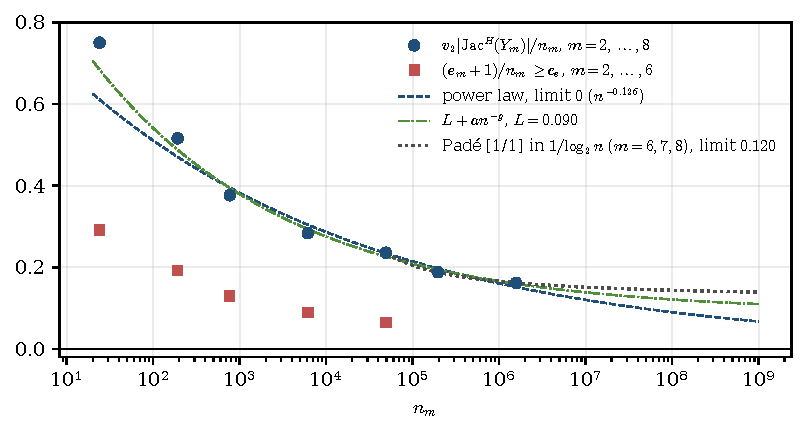
\includegraphics[width=\textwidth]{figures/fig_v2_growth.pdf}
\caption{The $2$-part of the Hecke Jacobian along the canonical $2$-tower: $v_2|\JacH(Y_m)|/n_m$ for
$m=2,\dots,8$ (Theorems~\ref{V3P6:thm:v2five}, \ref{V3P6:thm:v2eight}) and the normalized
$\F_2$-kernel dimensions $(e_m+1)/n_m$ for $m=2,\dots,6$, which decrease to the limit $c_e$
(Proposition~\ref{V3P6:prop:schur}, Theorem~\ref{V3P6:thm:v2sharp}). Three extrapolations of
$v_2/n_m$ that fit the data about equally well: a power law $n^{-0.126}$ with limit $0$ (fitted on
$m=3,\dots,8$); the least-squares optimum $0.090+an^{-g}$ of Remark~\ref{V3P6:rem:v2eight}(b); and the
Pad\'e approximant $[1/1]$ in $1/\log_2n$ through $m=6,7,8$, with limit $0.120$, drawn only on the range
of its data and beyond. The data do not decide between a positive limit and slow decay to $0$; what is
proved is $\liminf v_2/n_m\ge c_e$. Data of \texttt{code/v3p6\_level5\_v2.py}, drawn by
\texttt{code/make\_figures.py}.}
\label{V3P6:fig:v2growth}
\end{figure}

\begin{remark}[The data at levels $2$--$8$]\label{V3P6:rem:v2eight}
The numbers below are produced by lines (FT) and (E) of the script
\texttt{code/v3p6\_level5\_v2.py}.
\begin{enumerate}
\item[(a)] The sequences, with the local exponent
$\beta_m=\log\bigl(v_2(m)/v_2(m-1)\bigr)/\log(n_m/n_{m-1})$ and the ratio
$\rho_m=\bigl((e_m+1)/n_m\bigr)/\bigl((e_{m-1}+1)/n_{m-1}\bigr)$:
\begin{center}\small
\begin{tabular}{lccccccc}
\toprule
$m$ & $2$ & $3$ & $4$ & $5$ & $6$ & $7$ & $8$\\
\midrule
$n_m/n_{m-1}$ & --- & $8$ & $4$ & $8$ & $8$ & $4$ & $8$\\
$v_2/n_m$ & $0.750$ & $0.516$ & $0.376$ & $0.284$ & $0.236$ & $0.188$ & $0.162$\\
$\beta_m$ & --- & $0.820$ & $0.773$ & $0.864$ & $0.912$ & $0.836$ & $0.928$\\
$(e_m+1)/n_m$ & $0.292$ & $0.193$ & $0.130$ & $0.089$ & $0.064$ & & \\
$\rho_m$ & --- & $0.661$ & $0.676$ & $0.684$ & $0.724$ & & \\
\bottomrule
\end{tabular}
\end{center}
$v_2/n_m$ still decreases at every level, and every $\beta_m$ is below $1$. But the exponents are
increasing; along the layers of index $8$ they are $0.820$, $0.864$, $0.912$, $0.928$. Likewise
$(e_m+1)/n_m$ decreases with increasing ratios $\rho_m$, so the geometric decay by a constant factor
suggested by Remark~\ref{V3P6:rem:v2verdict}(b) is not borne out (Figure~\ref{V3P6:fig:v2growth}).
\item[(b)] \emph{Fits.} With limit $L=0$ the best power law is $v_2\sim n^{0.874}$. The
three-parameter model $v_2/n=L+an^{-g}$ fitted on $m=3,\dots,8$ has its least-squares optimum at
$L=0.090$, but the residual at $L=0$ is only $1.09$ times the optimum, and the leave-one-out optima
range over $[0,0.125]$. Exact fits through three consecutive levels jump with the period-$3$
pattern of the indices ($8,4,8,8,4,8$) and are not used. The data do not distinguish a positive
limit of order $0.1$ from slow decay to $0$.
\item[(c)] \emph{Rigorous interval.} $c_e\le\liminf v_2/n_m\le\limsup v_2/n_m\le h_H/\log2=2.977$,
with $0\le c_e\le0.0645$. The bound of Theorem~\ref{V3P6:thm:v2sharp} is far from sharp at finite
level: over $Y_4$ it gives $v_2/n_m\ge0.134,0.131,0.130$ for $m=6,7,8$, against the actual
$0.236,0.188,0.162$.
\item[(d)] \emph{The ratio to $c_e$.} At $m=2k$ the observed quotient
$\bigl(v_2|\JacH(Y_{2k})|/n_{2k}\bigr)\big/\bigl((e_k+1)/n_k\bigr)$ is $1.290,1.224,1.243$ for
$k=2,3,4$: on average a twisted block has about $1.25$ times the minimal valuation $e_k+1$. If this
quotient stays bounded, which would follow from a uniform bound on the $2$-exponents of the blocks
(they are at most $10$ at levels $6$--$8$), then $v_2|\JacH(Y_m)|/n_m$ and $(e_{\lceil m/2\rceil}+1)/n_{\lceil m/2\rceil}$ have the same
order, and $\lim v_2/n_m>0$ iff $c_e>0$.
\end{enumerate}
\emph{Verdict.} Strict positivity of the slope is not decided by levels $2$--$8$. What is proved is
that a positive mod-$2$ kernel density $c_e$ forces slope at least $c_e$; the numbers agree with
slope $\asymp c_e$, and both sequences are still decreasing, but more slowly at every level.
The open problem remains whether $c_e=\lim\dim_{\F_2}(\F_2[G_m]/\F_2[G_m]F_m)/n_m$ vanishes.
\end{remark}

\begin{remark}[Verification]\label{V3P6:rem:v2code}
The script \texttt{code/v3p6\_v2\_growth.py} uses numpy and the sparse module of scipy. It runs
in about five minutes (one minute with \texttt{--quick}, which skips line (FD)). It builds
levels $2$--$5$ (line (LV)), checks
the central elementary abelian layers and the voltages, the trace identities and the Hadamard
decomposition (BL), the valuation identity at the layers $2\to3$, $3\to4$ against the direct
values and its application at $4\to5$ (V2), the agreement of the $2$-adic eliminations with the
exact Smith forms at levels $2,3$ (SM), $e_m$ from the $\F_2$-rank of $I+A_1$ and from
$\dim C_m$ (E), the depth of $F_m$ (AU), the two automorphisms and their action on the
characters (SY), the total order and $v_2\le\log_2|\JacH|$ (TO), the direct elimination of the
$6144\times6144$ matrix (FD), and the table and growth statistics (TB), (GR).

The script \texttt{code/v3p6\_level5\_v2.py} (numpy, matplotlib; about three minutes, plus about
$70$ minutes with \texttt{--check7}) verifies Proposition~\ref{V3P6:prop:induced} and
Theorems~\ref{V3P6:thm:v2eight}, \ref{V3P6:thm:v2sharp}: the quotient models and the
elementary abelian structure of $P_k/P_m$ (QT), the conjugation orbits on the characters (CJ), the
re-derivation of $18,99,289$ by direct elimination and of $99,289,1742$ through induced characters
(VA), the new levels with the two routes to level $6$ (and, with \texttt{--check7}, the route to
level $7$ over $Y_5$) (NW), $e_m+1$ for $m\le6$ and the sharpened bound (E), the total orders (TO),
and the fits (FT). Data and the figure are written to \texttt{data/}.
\end{remark}

% Volume III, Chapter 6 -- addendum: localization over the non-analytic group ring Z_2[[P]]
% (open problem (a) of Section~\ref{V3P6:sec:retro}).  Verified by code/v3p6_pro2_localization.py
% and, for the 2-adic orders, code/v3p6_level5_v2.py.
\section{Localization over the non-analytic group \texorpdfstring{$\Z_2[[P]]$}{Z2[[P]]}}\label{V3P6:sec:pro2}

Corollary~\ref{V3P6:cor:status} leaves parts (i$'$) and (ii) of Theorem~\ref{V3P6:thm:main} open
for the canonical tower, because nothing is known about $\Lambda=\Z_2[[P]]$ beyond what holds for
every pro-$2$ group. This section separates what can be proved about $\Lambda$ from what cannot,
and proves an unconditional substitute for (ii): a compatible system of characteristic elements
at the finite levels, whose boundaries are the finite parts of the Iwasawa module and whose
reduced norms are the Artin factors of the class number formula. Throughout, $G_m=P/P_m$,
$n_m=3|G_m|$, $N_m=\sum_{g\in G_m}g\in\Z_2[G_m]$, and $\DeltaH_\Lambda\in M_3(\Lambda)$ is the
equivariant operator of Section~\ref{V3P6:sec:main} for the tower $Y_m\to X_3$, so that
$\Z_2[G_m]\otimes_\Lambda\DeltaH_\Lambda=\DeltaH(Y_m)\otimes\Z_2$ under
$\Z_2[G_m]^{3}=\Z_2^{V(Y_m)}$.

\subsection*{What is known about \texorpdfstring{$\Lambda$}{Lambda}}

\begin{proposition}[The group $P$ and its ring]\label{V3P6:prop:pro2basic}
\begin{enumerate}
\item[(i)] $P$ is a torsion-free pro-$2$ group, topologically generated by $3$ elements, of
infinite rank; $d(P_k)\ge2k$.
\item[(ii)] $\Lambda=\varprojlim_m\Z_2[G_m]$ is a compact local ring with maximal ideal
$(2,I_P)$, $I_P$ the augmentation ideal, and every finitely generated compact
$\Lambda$-module $M$ satisfies $M=\varprojlim_m\Z_2[G_m]\otimes_\Lambda M$.
\item[(iii)] The necessary condition for $\Lambda$ to be a domain holds: $\Z_2[[P]]$ has no
zero divisor of the form $(g-1)\nu$ with $g$ of finite order and $\nu$ its norm element.
\end{enumerate}
\end{proposition}

\begin{proof}
(i) Generation, rank and $d(P_k)$ are Theorem~\ref{V3P6:thm:tower}. A pro-$2$ group has no
torsion of odd order, so let $x\in1+\varphi\mathcal O$ with $x^{2^{k}}\in K^{\times}$,
$K=\F_2((t))$ the centre of $D_0$. The field $K(x)\subseteq D_0$ has degree $1$ or $3$ over $K$,
since $D_0$ is a division algebra of degree $3$. Over $K(x)$, in characteristic $2$, $y^{2^{k}}-x^{2^{k}}=(y-x)^{2^{k}}$, and the minimal
polynomial $f$ of $x$ over $K$ divides it, so $f=(y-x)^{j}$ with $j=[K(x):K]\in\{1,3\}$. If $j=3$,
then $f=y^{3}+xy^{2}+x^{2}y+x^{3}$ has its coefficients in $K$, so $x\in K$, a contradiction.
Hence $j=1$, $x\in K^{\times}\cap(1+\varphi\mathcal O)=1+t\F_2[[t]]$, and $x$ is
trivial in $P$. (ii) is standard for pro-$p$ groups: $\Lambda/(2,I_P)=\F_2$, and every element
outside $(2,I_P)$ is a unit, being a unit in every $\Z_2[G_m]$, which is local because $G_m$ is
a $2$-group; the limit statement holds because $M$ is a quotient of $\Lambda^{r}$ and inverse
limits of compact modules are exact. (iii) If $g$ has order $p$, then
$(g-1)(1+g+\dots+g^{p-1})=0$; by (i) there is no such $g\ne1$.
\end{proof}

The ring-theoretic questions that (i$'$) and (ii) need are open for $\Lambda$.

\begin{remark}[What is not known]\label{V3P6:rem:pro2open}
\begin{enumerate}
\item[(a)] \emph{Domain.} Neumann's theorem \cite{Neu88} says that $\Z_p[[G]]$ is a domain when
$G$ is a torsion-free \emph{$p$-adic analytic} pro-$p$ group; its proof goes through Lazard's
filtration and the fact that the associated graded ring is a polynomial ring \cite{Laz65}. $P$ is
not analytic (Theorem~\ref{V3P6:thm:tower}(iii)), so the theorem does not apply.
Proposition~\ref{V3P6:prop:pro2basic}(i) supplies the necessary condition, torsion-freeness, but
we know of no theorem that makes $\Z_2[[P]]$ a domain. Lazard's argument would go through if the
graded ring of $\F_2[[P]]$ for the filtration induced by the $P_m$ were a domain. The $P_m$ form a
restricted $N$-series, so by Jennings and Quillen this graded ring is the restricted enveloping
algebra of the graded restricted Lie algebra $\operatorname{gr}P$. In $\operatorname{gr}P$ the
squaring map is injective on every homogeneous piece: the square of $1+a\varphi^{k}$ is
$1+a\sigma^{k}(a)\varphi^{2k}$, and $a\sigma^{k}(a)$ is nonzero modulo the centre. So the obvious
source of zero divisors, $x^{[2]}=0$, is absent, but whether the enveloping algebra is a domain is
not known to us.
\item[(b)] \emph{Fractions.} Even for a domain, the nonzero elements need not form an Ore set.
Goldie's theorem gives the skew field $Q(\Lambda)$ for Noetherian domains, and whether
$\Z_2[[P]]$ is Noetherian is open (Corollary~\ref{V3P6:cor:status}); to our knowledge no pro-$p$ group of
infinite rank is known to have a Noetherian completed group ring. The Cohn localization at $\Sigma=\Lambda\setminus\{0\}$
exists by its universal property, but the localization sequence of
Definition~\ref{V3P6:def:cohn} needs $\Lambda\to\Sigma^{-1}\Lambda$ to be injective and stably flat,
which we cannot verify.
\item[(c)] \emph{Consequence.} The element $\mathcal L=[\DeltaH_\Lambda]\in K_1(Q(\Lambda))$ and the
identity $\partial\mathcal L=[X(Y/P)]$ are available only conditionally. Theorem~\ref{V3P6:thm:main}(i)
does hold unconditionally: $\DeltaH_\Lambda$ is injective on $\Lambda^{3}$.
\end{enumerate}
\end{remark}

\subsection*{An unconditional substitute: the tower of finite characteristic elements}

The trivial representation is the only obstruction at a finite level, so we remove it. Put
\[
A_m=\Z_2[G_m]/\Z_2N_m,\qquad \alpha_m=\text{image of }\DeltaH_\Lambda\text{ in }M_3(A_m),
\qquad X_m^{\mathrm{nt}}=\coker\bigl(\alpha_m\colon A_m^{3}\to A_m^{3}\bigr).
\]
$A_m$ is a ring, because $\Z_2N_m$ is a two-sided ideal ($gN_m=N_mg=N_m$). It is a $\Z_2$-order
in the semisimple algebra $\Q_2A_m=(1-e_m)\Q_2[G_m]=\bigoplus_{\rho\ne1}$, where
$e_m=N_m/|G_m|$ is the trivial idempotent; in particular $A_m$ is Noetherian, free of rank
$|G_m|-1$ over $\Z_2$, and $\Q_2A_m=A_m[\tfrac12]$ is its localization at the central
multiplicative set $\{2^{k}\}$. For such an order the localization sequence is classical and
unconditional:
\[
K_1(A_m)\to K_1(\Q_2A_m)\xrightarrow{\ \partial\ }K_0(A_m,\Q_2)\to K_0(A_m)\to K_0(\Q_2A_m),
\]
where $K_0(A_m,\Q_2)$ is the Grothendieck group of finite $A_m$-modules of projective dimension
$\le1$ and $\partial[\alpha]=[\coker\alpha]$ for injective $\alpha\in M_r(A_m)$, with the sign
convention of Definition~\ref{V3P6:def:cohn}.

\begin{lemma}[The rings $A_m$ form the tower]\label{V3P6:lem:pro2limit}
The projections $G_{m+1}\to G_m$ induce surjective ring maps $\pi_m\colon A_{m+1}\to A_m$ with
$\pi_m(\alpha_{m+1})=\alpha_m$, and $\Lambda\to\varprojlim_mA_m$ is an isomorphism of
topological rings.
\end{lemma}

\begin{proof}
$N_{m+1}\mapsto|P_m/P_{m+1}|\,N_m=2^{d_m}N_m$, so the ideal $\Z_2N_{m+1}$ maps into $\Z_2N_m$,
and $\pi_m$ is well defined and surjective. Both $\alpha_{m+1}$ and $\alpha_m$ are images of
$\DeltaH_\Lambda$. If $\lambda\in\Lambda$ maps to $0$ in every $A_m$, its images in
$\Z_2[G_m]$ are $c_mN_m$ with $c_m=2^{d_m}c_{m+1}$, so $c_m$ is divisible by every power of $2$,
and $\lambda=0$. Surjectivity follows from compactness, since all transition maps are
surjective.
\end{proof}

\begin{theorem}[Finite characteristic elements along the canonical tower]\label{V3P6:thm:pro2}
For every $m\ge1$, unconditionally:
\begin{enumerate}
\item[(i)] $\alpha_m$ is invertible in $M_3(\Q_2A_m)$, the sequence
$0\to A_m^{3}\xrightarrow{\alpha_m}A_m^{3}\to X_m^{\mathrm{nt}}\to0$ is exact, and
\[
X_m^{\mathrm{nt}}=\coker\bigl[\DeltaH(Y_m)\otimes\Z_2\ \big|\ \mathbf 1_{V_0},\mathbf 1_{V_1},
\mathbf 1_{V_2}\bigr]
\]
is a finite $A_m$-module of projective dimension $\le1$, where $\mathbf 1_{V_s}$ is the indicator
of the vertices of type $s$.
\item[(ii)] $\mathcal L_m:=[\alpha_m]\in K_1(\Q_2A_m)$ satisfies $\partial\mathcal L_m=[X_m^{\mathrm{nt}}]$,
and any $\mathcal L'\in K_1(\Q_2A_m)$ with $\partial\mathcal L'=[X_m^{\mathrm{nt}}]$ differs from
$\mathcal L_m$ by an element of the image of $K_1(A_m)$.
\item[(iii)] (Compatibility.) $\pi_{m*}\mathcal L_{m+1}=\mathcal L_m$ and
$A_m\otimes_{A_{m+1}}X_{m+1}^{\mathrm{nt}}\cong X_m^{\mathrm{nt}}$ with
$\operatorname{Tor}_1^{A_{m+1}}(A_m,X_{m+1}^{\mathrm{nt}})=0$, so the boundaries are compatible:
$\pi_{m*}\partial\mathcal L_{m+1}=\partial\mathcal L_m$. Hence
\[
\mathcal L_\infty:=(\mathcal L_m)_m\in\varprojlim_mK_1(\Q_2A_m),\qquad
X(Y/P)=\coker\DeltaH_\Lambda\cong\varprojlim_mX_m^{\mathrm{nt}} .
\]
\item[(iv)] (Artin descent.) Over $\C$, $\Q_2A_m\otimes\C=\bigoplus_{\rho\ne1}M_{\dim\rho}(\C)$ and
the reduced norm of $\mathcal L_m$ has components $\det\DeltaH_\rho$, $\rho\ne1$. The order of the
boundary is the class number formula:
\[
\log_2|X_m^{\mathrm{nt}}|=v_2\prod_{\rho\ne1}\det(\DeltaH_\rho)^{\dim\rho}
=v_2\Bigl([P:P_m]\,\frac{|\JacH(Y_m)|}{|\JacH(X_3)|}\Bigr)
=\log_2|G_m|+v_2|\JacH(Y_m)| .
\]
\end{enumerate}
\end{theorem}

\begin{proof}
(i) $\Q_2A_m\otimes\C$ is the sum of the nontrivial isotypic components of $\C[G_m]$, and on the
$\rho$-component $\alpha_m$ acts as $\DeltaH_\rho$ (with multiplicity $\dim\rho$), which is
nonsingular by Theorem~\ref{V3P6:thm:main}(iv). So $\alpha_m$ is invertible over $\Q_2A_m$ and
injective on the lattice $A_m^{3}$, whose cokernel is then finite; the exact sequence is a
resolution of length $1$ by free modules. Under $\Z_2[G_m]^{3}=\Z_2^{V(Y_m)}$ the element $N_me_s$
is $\mathbf 1_{V_s}$, so $A_m^{3}=\Z_2^{V(Y_m)}/\langle\mathbf 1_{V_0},\mathbf 1_{V_1},\mathbf 1_{V_2}\rangle$
and $X_m^{\mathrm{nt}}=\Z_2^{V(Y_m)}/(\operatorname{im}\DeltaH(Y_m)+\langle\mathbf 1_{V_s}\rangle)$.

(ii) is the definition of $\partial$ and the exactness of the localization sequence at
$K_1(\Q_2A_m)$.

(iii) $\pi_m(\alpha_{m+1})=\alpha_m$ by Lemma~\ref{V3P6:lem:pro2limit}. Applying
$A_m\otimes_{A_{m+1}}-$ to the resolution of (i) gives $A_m^{3}\xrightarrow{\alpha_m}A_m^{3}\to
A_m\otimes X_{m+1}^{\mathrm{nt}}\to0$, and $\alpha_m$ is injective, so the Tor term vanishes and
the base change is $X_m^{\mathrm{nt}}$. The localization sequences are natural for the ring map
$\pi_m$, which sends $2$ to $2$, so $\partial$ commutes with $\pi_{m*}$ (on $K_0(-,\Q_2)$ the map is
$[M]\mapsto[A_m\otimes^{\mathbf L}M]$). For the limit, $X=\varprojlim X_m$ with
$X_m=\Z_2[G_m]\otimes_\Lambda X=\coker\DeltaH(Y_m)\otimes\Z_2$
(Proposition~\ref{V3P6:prop:pro2basic}(ii)), and $X_m\to X_m^{\mathrm{nt}}$ is surjective with kernel
$K_m$, the $\Z_2$-span of the images of the $\mathbf 1_{V_s}$. The transition maps send
$\mathbf 1_{V_s}(Y_{m+1})\mapsto2^{d_m}\mathbf 1_{V_s}(Y_m)$, so a compatible family in $(K_m)$
lies in $\bigcap_j2^{j}K_m=0$ (Krull, $K_m$ being a finitely generated $\Z_2$-module); hence
$\varprojlim K_m=0$, and $\varprojlim X_m\cong\varprojlim X_m^{\mathrm{nt}}$ because $\varprojlim$
is exact on compact modules.

(iv) The first statement is the decomposition used in (i). For the order: $A_m^{3}$ is a free
$\Z_2$-module of rank $3(|G_m|-1)$, and for an injective endomorphism of a lattice
$|\coker\alpha_m|=|\det_{\Q_2}\alpha_m|_2^{-1}$. The $\Q_2$-determinant of $\alpha_m$ on
$\Q_2A_m^{3}$ is the determinant of $\DeltaH(Y_m)$ on the nontrivial isotypic part, i.e.\
$\prod_{\rho\ne1}\det(\DeltaH_\rho)^{\dim\rho}$, which equals $[P:P_m]|\JacH(Y_m)|/|\JacH(X_3)|$
by Theorem~\ref{V3P6:thm:main}(iv). Finally $|\JacH(X_3)|=147$ is odd.
\end{proof}

\begin{remark}[The orders, and the checks]\label{V3P6:rem:pro2check}
With Theorems~\ref{V3P6:thm:v2five} and~\ref{V3P6:thm:v2eight}, (iv) gives
$\log_2|X_m^{\mathrm{nt}}|=3+18=21$, $6+99=105$, $8+289=297$, $11+1742=1753$, $14+11595=11609$,
$16+36937=36953$ and $19+254662=254681$ for $m=2,\dots,8$. Over $\Z$ the same construction gives
$|X_2^{\mathrm{nt}}|=8\cdot|\JacH(Y_{24})|/147=2^{21}7^{14}$, which is the product of the seven
twisted determinants of the layer $Y_2\to Y_1$. The script \texttt{code/v3p6\_pro2\_localization.py}
(numpy; about three minutes) checks the ingredients at the levels $m\le5$: the orders $|G_m|$ and
the central elementary abelian layers (OR); the push-forward and pull-back identities
$\Pi\,\DeltaH(Y_{m+1})=\DeltaH(Y_m)\,\Pi$ and $\DeltaH(Y_{m+1})\Pi^{t}=\Pi^{t}\DeltaH(Y_m)$ behind
Lemma~\ref{V3P6:lem:pro2limit} (PF); the block decomposition of each layer (BL); the sector lemma
for all twisted blocks (SE); the Smith forms $\coker\DeltaH(Y_m)=\Z\oplus\JacH(Y_m)$ and the order
$|X_m^{\mathrm{nt}}|=|G_m||\JacH(Y_m)|/147$ over $\Z$ for $m=2,3$ (SM); the relative class number
formula of the layers $Y_2/Y_1$, $Y_3/Y_2$ and $Y_4/Y_3$ with exact integers, $|\JacH(Y_4)|$ being
reconstructed by Chinese remaindering (CN); and the surjectivity of
$\JacH(Y_{m+1})\to\JacH(Y_m)$ with kernel of order $\prod_{\chi\ne1}\det\DeltaH_\chi/|H_m|$ (KR).
\end{remark}

\begin{remark}[How far this goes]\label{V3P6:rem:pro2scope}
Theorem~\ref{V3P6:thm:pro2} is the form of Theorem~\ref{V3P6:thm:main}(i$'$),(ii) that holds without
knowing anything about $\Z_2[[P]]$: the characteristic element lives in the inverse limit
$\varprojlim K_1(\Q_2A_m)$ instead of $K_1(Q(\Lambda))$, its boundary is the system of finite
modules $X_m^{\mathrm{nt}}$ whose limit is $X(Y/P)$, and its reduced norms are the Artin factors. This
is the shape of the finite-level formulations of non-commutative Iwasawa theory, where $K_1$ of a
localized Iwasawa algebra is approached through the finite group rings. If $\Lambda$ turns out to be
an Ore domain, then $\mathcal L=[\DeltaH_\Lambda]\in K_1(Q(\Lambda))$ exists and
$\partial\mathcal L=[X]$ by Theorem~\ref{V3P6:thm:main}(ii); we do not claim a map relating
$\mathcal L$ to $\mathcal L_\infty$, because a skew field of fractions of $\Lambda$ need not map to
the finite-level algebras $\Q_2A_m$. Open
problem (a) of Section~\ref{V3P6:sec:retro} is therefore sharpened to: is $\Z_2[[P]]$ a Noetherian
domain, or at least an Ore domain?
\end{remark}

\begin{remark}[Corrections to the proposed programme]\label{V3P6:rem:pro2corrections}
(1) Neumann's theorem does not say that $\Z_2[[P]]$ is a domain: it requires a $p$-adic analytic
group, and $P$ is not one. What is proved is that $P$ is torsion-free
(Proposition~\ref{V3P6:prop:pro2basic}), which is necessary, not sufficient. (2) The Ore
localization at $\Lambda\setminus\{0\}$, i.e.\ the skew field $Q(\Lambda)$, is not known to exist:
Goldie's theorem needs a Noetherian ring (Remark~\ref{V3P6:rem:pro2open}). (3) Therefore
$\partial[\DeltaH_\Lambda]=[X(Y/P)]$ in $K_1(Q(\Lambda))$ is not proved unconditionally. What holds
unconditionally is Theorem~\ref{V3P6:thm:pro2}, the same identity at every finite level, compatibly
along the tower, with $X(Y/P)$ recovered as the limit. (4) The descent formula with denominator
$|\JacH(X_3)|$ is Theorem~\ref{V3P6:thm:main}(iv); in Theorem~\ref{V3P6:thm:pro2}(iv) it computes the
order of the boundary. (5) $d(P_k)\ge2k$ and the absence of the Ore set of \cite{CFKSV} are
Theorems~\ref{V3P6:thm:tower}(iii) and~\ref{V3P6:thm:nozp}, as stated in the proposed programme.
\end{remark}


\section{Verification battery}\label{V3P6:sec:battery}

\begin{table}[ht]
\centering\scriptsize
\renewcommand{\arraystretch}{1.2}
\resizebox{\textwidth}{!}{%
\begin{tabular}{lcl}
\toprule
check & complexes & result\\
\midrule
(Dg) polynomial representation of $\mathbb H_2$ (degree $\le4$); trivial module with $x_1=L_E(Y_{21})$ & --- & exact / numeric\\
(Hq) $T_i^{2}=(q-1)T_i+q$, braid relations & $Y_{21},Y_{24},Y_{168},T_6$ & exact\\
(Op) $\Delta_2=3+\sum T_i$; $A_1=(q+1)^{-1}\sum\pi_t\pi_{t+1}^{t}$; $L_E=p\,T_tT_{t+2}T_t\,p^{t}/(q(q+1))$ & $Y_{21},Y_{168}$ & exact\\
(Sa) $a=qe_1(z)$, $\bar a=qe_2(z)$, $e_3=1$; $\DeltaH$ as symmetric polynomial & $Y_{42},Y_{168}$ & numeric $10^{-8}$\\
(CN) $\prod_{\chi\ne1}\det\DeltaH_\chi=|A||\JacH(Y_A)|/|\JacH(X_3)|$ & $Y_{21},Y_{24},Y_{42}$ & numeric vs exact Smith forms\\
(B1) $b_1=0$, hence no $\Z_p$-quotient & five covers & exact\\
\midrule
\multicolumn{3}{l}{\texttt{code/v3p6\_deep\_verify.py}}\\
(CS) $x+2y+4z\equiv0$ on $T$; $u_xu_yu_z=1+t$ & --- & exact\\
(NB) the $7$ hyperplanes, $7$ lines and their incidence $=$ link of the CMSZ building, for every $\bar e$ & --- & exact\\
(FR) generators span $P/P_2=\F_8$; squares and commutators fill levels $2..13$ & --- & exact\\
(IM) image of $\Gamma^{0}$ $=$ $P/P_m$ for $m\le6$; lower bounds for $d(P_k)$ & --- & exact\\
(L2) level $2$ has $\JacH(Y_{24})$ & $Y_2$ & exact\\
(J) $v_2|\JacH|=18,99,289$; $\frac1n\log|\JacH|=1.8629,2.0416,2.0544$; Ramanujan; $\min\operatorname{Re}\mu>0$ & $Y_2,Y_3,Y_4$ & exact / numeric\\
(PL) Plancherel moments $|a|^{2}\mapsto7$, $a^{3}\mapsto21$; $h_H(2)=2.063693$ & --- & numeric $10^{-6}$\\
\bottomrule
\end{tabular}}
\medskip
\caption{Checks run by \texttt{code/v3p6\_verify.py}.}
\label{V3P6:tab:battery}
\end{table}

\section{Corrections}\label{V3P6:sec:scope}

\begin{remark}[Corrections to the proposed programme]\label{V3P6:rem:corrections}
(1) ``Strictly realized as a representation of $\mathbb H_d$'' is vacuous
(Proposition~\ref{V3P6:prop:reps}(ii)). The natural structure is $H_q$ on chambers
(Theorems~\ref{V3P6:thm:iwahori}, \ref{V3P6:thm:ops}), and the Kuramoto field is not linear.
(2) The localization sequence ends in $\to0$ only under an injectivity condition on $K_0$. The
set $\Sigma$ of the proposed programme is not the Ore set of \cite{CFKSV}, and that Ore set does not
exist over thick complexes (Theorem~\ref{V3P6:thm:nozp}). (3) An ``unconditional'' $L$-element
requires a tower, which is Hypothesis~(T); the element is then $[\DeltaH_\Lambda]$, and
$\det(I-uC^{(3)})$ enters through its specializations (Theorem~\ref{V3P6:thm:main}(v)). (4)
$\mathrm{Sel}(Y/G)$ is undefined. With $X(Y/G)$ in its place the ``main conjecture'' is a
theorem, and its content is descent and the class number formula. (5) The five-step scheme is
not a proof (Section~\ref{V3P6:sec:five}). (6) Nothing in Volume~III supports a
cosmological reading. (7) (Deepening request.) $\Gamma$ is discrete in
$\PGL_3(\F_2((s)))$, so the proposed map $\Gamma\to\PGL_3(\mathcal O_K/\mathfrak p^{m})$ at that
place does not exist. Congruence towers come from other places of $\F_2(t)$. In
characteristic $2$ their groups have infinite rank, so they are not ``uniform pro-$p$ with Lie
algebra $\mathfrak{pgl}_3$''. What is unconditional is (T$_2$) and the parts of
Theorem~\ref{V3P6:thm:main} that need only it (Corollary~\ref{V3P6:cor:status}). An ``exact
asymptotic formula'' is proved for the total order (Theorem~\ref{V3P6:thm:growth}), not for the
$2$-part.
\end{remark}

\section*{Acknowledgement of provenance and caveats}

Unrefereed. The inputs quoted without proof are the structure theory of $\mathbb H_d$
\cite{Dri86,Lus89}, the Iwahori--Hecke algebra \cite{IM65}, Cohn localization and its
$K$-theory \cite{Coh85,NR04}, Lazard's and Neumann's theorems on $\Z_p[[G]]$ \cite{Laz65,Neu88},
and the framework of \cite{CFKSV}, which is used only to explain why it does not apply. The
bibliographic data of \cite{Dri86,Lus89,IM65,Coh85,NR04,Neu88} have been checked against Crossref and zbMATH.



\backmatter
% State of Volume III -- one \item per chapter; labels of Volumes I--II are read through xr
% with the prefix M- (see ANCCFT_Volume_III.tex).
\chapter*{State of Volume III}
\addcontentsline{toc}{chapter}{State of Volume III}

\begin{itemize}
\item \textbf{Rank-two topology, proved locally} (Ch.~\ref{chap:V3P1}): the general cubic
trace identity $\Tr(\Cthree)^{3}=\Tr A_1^{3}-3q|E|+3nq^{3}$, which equals $n(q-1)^{2}(q+1)$
\emph{only under the flag condition} --- on $Y_{21}$ the true trace is $651$, of which $63$
is the flag part and $588$ comes from non-simplex $3$-cycles
(Thm.~\ref{V3P1:thm:trace}); Garland vanishing $H^{1}(Y;\mathcal E)=0$ for every unitary
local system, from the link gap $1-\sqrt q/(q+1)>\tfrac12$ alone, with no building, group
action or flag condition (Thm.~\ref{V3P1:thm:garland}); $\det(I-u\Cthree)=\det P(u)$ with
$1-u^{3}$ of multiplicity exactly $b_0=1$, the Betti numbers $b_1,b_2$ entering only on the
edge (branch) side of the Kang--Li zeta function (Thms.~\ref{V3P1:thm:det},
\ref{V3P1:thm:orbit}, Rem.~\ref{V3P1:rem:betti}); the sector lemma removing the hypothesis
of Vol.~I--II, Ch.~\ref{M-chap:X}, Thm.~\ref{M-X:thm:hecke}(ii); and the derivative identity
$\frac{d}{du}\det(I-u\Cthree)|_{u=1}=(-1)^{n}n(q-1)^{2}(q+1)|\JacH(Y)|$
(Thm.~\ref{V3P1:thm:deriv}).
\item \textbf{Simplicial sandpiles} (Ch.~\ref{chap:V3P2}): on thick complexes none of
$\Delta_1$, $\partial_2\partial_2^{t}$, $\Delta_2$, $\DeltaH$ can be switched to a Z-matrix, so
edge, chamber and Hecke toppling are not abelian and have no recurrent group; only the
vertex sandpile survives, and on thin tori the chamber sandpile is the honeycomb one
(Thm.~\ref{V3P2:thm:sign}, Cor.~\ref{V3P2:cor:nonabelian}). The Hodge factorization
$|\Jac_1|\operatorname{disc}\ker_\Z\Delta_1=n|\Jac_0||\Jac_2|\operatorname{disc}H_2(Y;\Z)$,
which reads $|\Jac_1|=\det\Delta_1$ on thick complexes (Thm.~\ref{V3P2:thm:hodge}). Exact
mean avalanche size $\langle s\rangle=n^{2}L^{+}_{ss}/(n-1)\in[n/\lambda_{\max},n/\lambda_2]$,
hence $\Theta(n)$ on expanding families against $\Theta(n\log n)$ on $2$D tori
(Thm.~\ref{V3P2:thm:mean}, Cor.~\ref{V3P2:cor:linear}); mean-field exponents conjectural
(Conj.~\ref{V3P2:conj:mf}). The $1$-skeleton of $Y_{21}$ is $K_{7,7,7}$
(Prop.~\ref{V3P2:prop:k777}).
\item \textbf{Phase oscillators} (Ch.~\ref{chap:V3P3}): chiral connections of any flux exist on
every $\Atwo$ complex and form a torsor under $\Hom(H_1,U(1))$, which has $64$ elements on
$Y_{21}$ (Prop.~\ref{V3P3:prop:chiral}). The flux sector is a gradient flow for every flux, so
there are no limit cycles and no Hopf bifurcation. Its ground states are twisted states
carrying static currents (Thms.~\ref{V3P3:thm:gradient}, \ref{V3P3:thm:ground}). For all
parameters the twisted states rotate at $\omega+K_2\sin\Phi$ with Jacobian $-c_m\Delta_0$
(Thm.~\ref{V3P3:thm:twisted}). The cluster subspace is gradient modulo rotation, and the
Jacobian at cluster states splits into $3\times3$ blocks, all real on $Y_{21}$
(Thms.~\ref{V3P3:thm:clustergrad}, \ref{V3P3:thm:blocks}). The Ott--Antonsen reduction closes
only for $K_2=0$, and then excludes chimeras for identical oscillators
(Prop.~\ref{V3P3:prop:oa}, Thm.~\ref{V3P3:thm:nochimera}); chimeras for $K_2\ne0$ remain open.
The geometric phase of a rigid rotation is $0$; flux threading permutes the twisted states
cyclically; and $\Delta\Omega$ does not involve $\chi(Y)$ (Prop.~\ref{V3P3:prop:monodromy},
Rem.~\ref{V3P3:rem:euler}).
\item \textbf{Geodesic edge operator} (Ch.~\ref{chap:V3P4}): $L_E$ is $q^{2}$-biregular and
block-cyclic. The subspace $S^{t}\C^{V}+T^{t}\C^{V}+Q\C^{V}$ is invariant and carries the Hecke
pencil (Thm.~\ref{V3P4:thm:vertex}). On its complement $W$, $L_E^{t}$ is exactly $\sqrt q$
times an isometry, unconditionally and for all $\Atilde d$ with $q^{(d-1)/2}$
(Thms.~\ref{V3P4:thm:unitary}, \ref{V3P4:thm:Ad}), and every eigenvalue has
$|\lambda|\ge\sqrt q$ (Thm.~\ref{V3P4:thm:lower}). $\det(I-uL_E)=\det
P(u)\det(I-u\bar L)/((1-u^{3})(1-q^{3}u^{3}))$ off an explicit exceptional curve, and the
two-circle Riemann hypothesis is equivalent to the Ramanujan property
(Thms.~\ref{V3P4:thm:factor}, \ref{V3P4:thm:ramanujan}). Degenerate spectra are not Poisson,
small perturbations do not give Wigner--Dyson statistics, and Brody $b=2$ is not GUE
(Props.~\ref{V3P4:prop:atom}--\ref{V3P4:prop:brody}).
\item \textbf{Chamber public-goods games} (Ch.~\ref{chap:V3P5}): the chamber game is an
additive pairwise game on the $1$-skeleton, with the flags entering only through $q+1$
(Thm.~\ref{V3P5:thm:reduction}). The mean-field threshold is $r_c=3$ for every $q$
(Prop.~\ref{V3P5:prop:mf}). Zero-noise cluster thresholds are $3\kappa/(\kappa+\delta)$ with
integer $\delta$, so $5/3$ never occurs for $q=2$, and $Y_{21}$ has no cages
(Thm.~\ref{V3P5:thm:cluster}, Prop.~\ref{V3P5:prop:Y21}). In Monte Carlo runs thick complexes
behave like random regular graphs, while the thin lattice favours cooperation
(Rem.~\ref{V3P5:rem:mc}). Cyclic replicator dynamics has no limit cycle and no torus, and
mutation produces a Hopf cycle at $\mu_H=(b-a)/18$ (Thms.~\ref{V3P5:thm:rps},
\ref{V3P5:thm:mutation}).
\item \textbf{Hecke algebras and Iwasawa theory} (Ch.~\ref{chap:V3P6}): realizing an operator
in a representation of the degenerate affine Hecke algebra is vacuous. The Iwahori--Hecke
algebra $H_q(\Atwo)$ acts on chambers under (L), and $\Delta_2$, $A_1$ and $L_E$ are expressed
through it (Prop.~\ref{V3P6:prop:reps}, Thms.~\ref{V3P6:thm:iwahori}, \ref{V3P6:thm:ops}).
Garland rigidity removes every $\Z_p$-direction, so the Ore set of Coates et al.\ is not
available (Thm.~\ref{V3P6:thm:nozp}). Under a tower hypothesis the equivariant Hecke--Laplacian
is injective, $\partial[\DeltaH_\Lambda]=[X]$, descent recovers the $\JacH(Y_U)$, and the class
number formula $\prod_{\rho\ne1}\det(\DeltaH_\rho)^{\dim\rho}=[G:U]|\JacH(Y_U)|/|\JacH(Y)|$ holds;
it equals $7^{18}$ on $Y_{21}$ (Thm.~\ref{V3P6:thm:main}). The presentation embeds in the cyclic division algebra $(\F_8(t)/\F_2(t),\mathrm{Frob},t)$ via $a_x\mapsto1+\alpha^{x}\varphi$, so the building is that of $\PGL_3(\F_2((s)))$ (Thm.~\ref{V3P6:thm:cs}). The resulting canonical pro-$2$ tower over $X_3$ is unconditional, starts with $Y_{24}$, and has a group of infinite rank that is not $p$-adic analytic (Thm.~\ref{V3P6:thm:tower}, Cor.~\ref{V3P6:cor:status}). $\frac1n\log|\JacH|\to h_H(2)=2.063693$ along any exhausting tower (Thm.~\ref{V3P6:thm:growth}).


\end{itemize}

\section*{Status at the close of Volume III}

The open problems carried by Chapter~\ref{chap:V3P6} (Section~\ref{V3P6:sec:retro}) stand as follows.
\begin{itemize}
\item[(a)] \emph{Towers.} Settled in the form in which it can be settled. The group of Vol.~I--II
is the Cartwright--Steger lattice of $\PGL_3(\F_2((s)))$, and its building is Bruhat--Tits. The
canonical pro-$2$ tower over $X_3$ exists unconditionally, starts with $Y_{24}$, and satisfies
(T$_2$). Hence Theorem~\ref{V3P6:thm:main}(i),(iii),(iv),(v) are unconditional. The tower is
\emph{not} $p$-adic analytic, and (T) is expected to fail for every tower
(Theorems~\ref{V3P6:thm:cs}, \ref{V3P6:thm:tower}, Corollary~\ref{V3P6:cor:status},
Remark~\ref{V3P6:rem:analytic}). $P$ is torsion-free, and the characteristic element exists
unconditionally as a compatible system $\mathcal L_\infty\in\varprojlim K_1(\Q_2A_m)$ with
boundaries the finite modules $X_m^{\mathrm{nt}}$, whose limit is $X(Y/P)$
(Theorem~\ref{V3P6:thm:pro2}). \emph{Still open:} whether $\Z_2[[P]]$ is an Ore domain, i.e.\ a
localization in which Theorem~\ref{V3P6:thm:main}(ii) holds.
\item[(b)] \emph{Growth of Hecke Jacobians.} Settled for the total order: along every exhausting
tower, $\frac1n\log|\JacH|\to h_H(2)=2.063693$, a Plancherel integral
(Theorem~\ref{V3P6:thm:growth}). For the $2$-part, $v_2|\JacH(Y_m)|$ is known exactly up to
$n=1572864$ (Theorem~\ref{V3P6:thm:v2eight}), and $\liminf v_2/n\ge c_e$ with $0\le c_e\le0.0645$
(Theorem~\ref{V3P6:thm:v2sharp}). \emph{Still open:} whether the slope is positive, i.e.\
essentially whether $c_e>0$ (Remark~\ref{V3P6:rem:v2eight}).
\item[(e)] \emph{Finite-noise thresholds and nonlinear chamber games.} Answered in Chapter~\ref{chap:V3P5},
Sections~\ref{V3P5:sec:nonlinear}--\ref{V3P5:sec:clocks}. Nonlinearity is exactly what makes a
chamber game irreducible. Symmetric games are potential games, so their selected state does not
depend on geometry. Chiral games break the potential and cycle in the mean field; on large
networks the cycle is coherent only when entrained by a synchronized clock. The thin-lattice
advantage is the flat interface, and finite anchors cannot remove the frontier threshold of
thick buildings. No ``topological catalysis'' by thickness exists. \emph{Still open:} the star
formula for $q\ge3$, and finite-noise phase transitions on infinite complexes.
\end{itemize}
Problems (c), (d) and (f) of that list remain open: the vertex block of $L_E$ for $\Atilde d$,
$d\ge3$ (the trace identity of (c) is settled: $\Tr(C^{(d+1)})^{d+1}=n\prod_{i=1}^{d}(1-q^{i})$ under
the flag condition, Theorem~\ref{V3P1:thm:tracead}); universality for the remainder eigenphases (on $Y_{168}$ the crossover to GUE and its
first-order scale are settled, Section~\ref{V3P4:sec:chaos}); and chimeras and transverse Hopf bifurcations
for the triadic lag. Of (f), the transverse Hopf bifurcations are found on $Y_{168}$: they have
multiplicity $21$, and in every case examined the loss of stability is hard and ends in a locked state
(Section~\ref{V3P3:sec:hopf}); whether some equivariant branch is supercritical, and the chimeras,
remain open. Volume~III closes with these results and these open problems.

\begin{thebibliography}{99}
\bibitem{CFKSV} J.~Coates, T.~Fukaya, K.~Kato, R.~Sujatha and O.~Venjakob, \emph{The $\mathrm{GL}_2$ main conjecture for elliptic curves without complex multiplication}, Publ.\ Math.\ Inst.\ Hautes \'Etudes Sci.\ \textbf{101} (2005), 163--208. \doi{10.1007/s10240-004-0029-3}

\bibitem{Dhar90} D.~Dhar, \emph{Self-organized critical state of sandpile automaton models}, Phys.\ Rev.\ Lett.\ \textbf{64} (1990), 1613--1616. \doi{10.1103/PhysRevLett.64.1613}

\bibitem{DM90} D.~Dhar and S.~N.~Majumdar, \emph{Abelian sandpile model on the Bethe lattice}, J.\ Phys.\ A \textbf{23} (1990), 4333--4350. \doi{10.1088/0305-4470/23/19/018}

\bibitem{DKM} A.~M.~Duval, C.~J.~Klivans and J.~L.~Martin, \emph{Critical groups of simplicial complexes}, Ann.\ Comb.\ \textbf{17} (2013), 53--70. \doi{10.1007/s00026-012-0168-z}

\bibitem{Harris63} T.~E.~Harris, \emph{The Theory of Branching Processes}, Grundlehren Math.\ Wiss.\ \textbf{119}, Springer, Berlin, 1963. \doi{10.1007/978-3-642-51866-9}

\bibitem{Lyons2005} R.~Lyons, \emph{Asymptotic enumeration of spanning trees}, Combin.\ Probab.\ Comput.\ \textbf{14} (2005), 491--522. \doi{10.1017/S096354830500684X}

\bibitem{DDMS} J.~D.~Dixon, M.~P.~F.~du~Sautoy, A.~Mann and D.~Segal, \emph{Analytic Pro-$p$ Groups}, 2nd ed., Cambridge Stud.\ Adv.\ Math.\ \textbf{61}, Cambridge Univ.\ Press, Cambridge, 1999. \doi{10.1017/CBO9780511470882}

\bibitem{Ga} H.~Garland, \emph{$p$-adic curvature and the cohomology of discrete subgroups of $p$-adic groups}, Ann.\ of Math.\ (2) \textbf{97} (1973), 375--423. \doi{10.2307/1970829}

\bibitem{BSw} W.~Ballmann and J.~\'Swi\k{a}tkowski, \emph{On $L^{2}$-cohomology and property (T) for automorphism groups of polyhedral cell complexes}, Geom.\ Funct.\ Anal.\ \textbf{7} (1997), 615--645. \doi{10.1007/s000390050022}

\bibitem{KL} M.-H.~Kang and W.-C.~W.~Li, \emph{Zeta functions of complexes arising from $\mathrm{PGL}(3)$}, Adv.\ Math.\ \textbf{256} (2014), 46--103. \doi{10.1016/j.aim.2013.12.033}

\bibitem{Laz65} M.~Lazard, \emph{Groupes analytiques $p$-adiques}, Publ.\ Math.\ Inst.\ Hautes \'Etudes Sci.\ \textbf{26} (1965), 5--219. \doi{10.1007/BF02684303}

\bibitem{Wei64} A.~Weil, \emph{Remarks on the cohomology of groups}, Ann.\ of Math.\ (2) \textbf{80} (1964), 149--157. \doi{10.2307/1970495}

\bibitem{AMSW08} D.~M.~Abrams, R.~Mirollo, S.~H.~Strogatz and D.~A.~Wiley, \emph{Solvable model for chimera states of coupled oscillators}, Phys.\ Rev.\ Lett.\ \textbf{101} (2008), 084103. \doi{10.1103/PhysRevLett.101.084103}

\bibitem{KB02} Y.~Kuramoto and D.~Battogtokh, \emph{Coexistence of coherence and incoherence in nonlocally coupled phase oscillators}, Nonlinear Phenom.\ Complex Syst.\ \textbf{5} (2002), 380--385.

\bibitem{LaSalle60} J.~P.~LaSalle, \emph{Some extensions of Liapunov's second method}, IRE Trans.\ Circuit Theory \textbf{7} (1960), 520--527. \doi{10.1109/TCT.1960.1086720}

\bibitem{Loj63} S.~\L{}ojasiewicz, \emph{Une propri\'et\'e topologique des sous-ensembles analytiques r\'eels}, in: Les \'Equations aux D\'eriv\'ees Partielles (Paris, 1962), Colloques Internat.\ CNRS \textbf{117}, \'Editions du CNRS, Paris, 1963, 87--89.

\bibitem{OA08} E.~Ott and T.~M.~Antonsen, \emph{Low dimensional behavior of large systems of globally coupled oscillators}, Chaos \textbf{18} (2008), 037113. \doi{10.1063/1.2930766}

\bibitem{SK86} H.~Sakaguchi and Y.~Kuramoto, \emph{A soluble active rotator model showing phase transitions via mutual entrainment}, Progr.\ Theoret.\ Phys.\ \textbf{76} (1986), 576--581. \doi{10.1143/PTP.76.576}

\bibitem{GSS88} M.~Golubitsky, I.~Stewart and D.~G.~Schaeffer, \emph{Singularities and Groups in Bifurcation Theory, Vol.~II}, Appl.\ Math.\ Sci.\ \textbf{69}, Springer, New York, 1988. \doi{10.1007/978-1-4612-4574-2}

\bibitem{SA19} P.~S.~Skardal and A.~Arenas, \emph{Abrupt desynchronization and extensive multistability in globally coupled oscillator simplexes}, Phys.\ Rev.\ Lett.\ \textbf{122} (2019), 248301. \doi{10.1103/PhysRevLett.122.248301}

\bibitem{Atas13} Y.~Y.~Atas, E.~Bogomolny, O.~Giraud and G.~Roux, \emph{Distribution of the ratio of consecutive level spacings in random matrix ensembles}, Phys.\ Rev.\ Lett.\ \textbf{110} (2013), 084101. \doi{10.1103/PhysRevLett.110.084101}

\bibitem{BGS84} O.~Bohigas, M.-J.~Giannoni and C.~Schmit, \emph{Characterization of chaotic quantum spectra and universality of level fluctuation laws}, Phys.\ Rev.\ Lett.\ \textbf{52} (1984), 1--4. \doi{10.1103/PhysRevLett.52.1}

\bibitem{Brody73} T.~A.~Brody, \emph{A statistical measure for the repulsion of energy levels}, Lett.\ Nuovo Cimento \textbf{7} (1973), 482--484. \doi{10.1007/BF02727859}

\bibitem{JMRR99} D.~Jakobson, S.~D.~Miller, I.~Rivin and Z.~Rudnick, \emph{Eigenvalue spacings for regular graphs}, in: Emerging Applications of Number Theory, IMA Vol.\ Math.\ Appl.\ \textbf{109}, Springer, New York, 1999, 317--327. \doi{10.1007/978-1-4612-1544-8_12}

\bibitem{KLW10} M.-H.~Kang, W.-C.~W.~Li and C.-J.~Wang, \emph{The zeta functions of complexes from $\mathrm{PGL}(3)$: a representation-theoretic approach}, Israel J.\ Math.\ \textbf{177} (2010), 335--348. \doi{10.1007/s11856-010-0049-2}

\bibitem{Kato} T.~Kato, \emph{Perturbation Theory for Linear Operators}, Grundlehren Math.\ Wiss.\ \textbf{132}, Springer, Berlin, 1966; reprint of the 2nd ed., Classics in Mathematics, Springer, Berlin, 1995. \doi{10.1007/978-3-642-66282-9}

\bibitem{KS97} T.~Kottos and U.~Smilansky, \emph{Quantum chaos on graphs}, Phys.\ Rev.\ Lett.\ \textbf{79} (1997), 4794--4797. \doi{10.1103/PhysRevLett.79.4794}

\bibitem{LSV05} A.~Lubotzky, B.~Samuels and U.~Vishne, \emph{Ramanujan complexes of type $\tilde A_d$}, Israel J.\ Math.\ \textbf{149} (2005), 267--299. \doi{10.1007/BF02772543}

\bibitem{Mob10} M.~Mobilia, \emph{Oscillatory dynamics in rock--paper--scissors games with mutations}, J.\ Theoret.\ Biol.\ \textbf{264} (2010), 1--10. \doi{10.1016/j.jtbi.2010.01.008}

\bibitem{NM92} M.~A.~Nowak and R.~M.~May, \emph{Evolutionary games and spatial chaos}, Nature \textbf{359} (1992), 826--829. \doi{10.1038/359826a0}

\bibitem{SPS09} A.~Szolnoki, M.~Perc and G.~Szab\'o, \emph{Topology-independent impact of noise on cooperation in spatial public goods games}, Phys.\ Rev.\ E \textbf{80} (2009), 056109. \doi{10.1103/PhysRevE.80.056109}

\bibitem{ST98} G.~Szab\'o and C.~T\H{o}ke, \emph{Evolutionary prisoner's dilemma game on a square lattice}, Phys.\ Rev.\ E \textbf{58} (1998), 69--73. \doi{10.1103/PhysRevE.58.69}

\bibitem{Coh85} P.~M.~Cohn, \emph{Free Rings and Their Relations}, 2nd ed., London Math.\ Soc.\ Monogr.\ \textbf{19}, Academic Press, London, 1985.

\bibitem{Dri86} V.~G.~Drinfeld, \emph{Degenerate affine Hecke algebras and Yangians}, Funct.\ Anal.\ Appl.\ \textbf{20} (1986), 58--60. \doi{10.1007/BF01077318}

\bibitem{IM65} N.~Iwahori and H.~Matsumoto, \emph{On some Bruhat decomposition and the structure of the Hecke rings of $p$-adic Chevalley groups}, Publ.\ Math.\ Inst.\ Hautes \'Etudes Sci.\ \textbf{25} (1965), 5--48. \doi{10.1007/BF02684396}

\bibitem{Lus89} G.~Lusztig, \emph{Affine Hecke algebras and their graded version}, J.\ Amer.\ Math.\ Soc.\ \textbf{2} (1989), 599--635. \doi{10.1090/S0894-0347-1989-0991016-9}

\bibitem{Neu88} A.~Neumann, \emph{Completed group algebras without zero divisors}, Arch.\ Math.\ \textbf{51} (1988), 496--499. \doi{10.1007/BF01261969}

\bibitem{NR04} A.~Neeman and A.~Ranicki, \emph{Noncommutative localisation in algebraic $K$-theory I}, Geom.\ Topol.\ \textbf{8} (2004), 1385--1425. \doi{10.2140/gt.2004.8.1385}

\bibitem{Mac71} I.~G.~Macdonald, \emph{Spherical Functions on a Group of $p$-adic Type}, Publ.\ Ramanujan Inst.\ \textbf{2}, Univ.\ of Madras, Madras, 1971.

\bibitem{Mar91} G.~A.~Margulis, \emph{Discrete Subgroups of Semisimple Lie Groups}, Ergeb.\ Math.\ Grenzgeb.\ (3) \textbf{17}, Springer, Berlin, 1991. \doi{10.1007/978-3-642-51445-6}

\bibitem{Opp18} I.~Oppenheim, \emph{Local spectral expansion approach to high dimensional expanders. Part I: Descent of spectral gaps}, Discrete Comput.\ Geom.\ \textbf{59} (2018), 293--330. \doi{10.1007/s00454-017-9948-x}

\bibitem{CS98} D.~I.~Cartwright and T.~Steger, \emph{A family of $\tilde A_n$-groups}, Israel J.\ Math.\ \textbf{103} (1998), 125--140. \doi{10.1007/BF02762271}

\bibitem{MS96} D.~Monderer and L.~S.~Shapley, \emph{Potential games}, Games Econom.\ Behav.\ \textbf{14} (1996), 124--143. \doi{10.1006/game.1996.0044}

\bibitem{MPS90} J.~Mallet-Paret and H.~L.~Smith, \emph{The Poincar\'e--Bendixson theorem for monotone cyclic feedback systems}, J.\ Dynam.\ Differential Equations \textbf{2} (1990), 367--421. \doi{10.1007/BF01054041}

\bibitem{Smith95} H.~L.~Smith, \emph{Monotone Dynamical Systems: An Introduction to the Theory of Competitive and Cooperative Systems}, Math.\ Surveys Monogr.\ \textbf{41}, Amer.\ Math.\ Soc., Providence, RI, 1995. \doi{10.1090/surv/041}

\bibitem{Zuk96} A.~\.Zuk, \emph{La propri\'et\'e (T) de Kazhdan pour les groupes agissant sur les poly\`edres}, C.~R.\ Acad.\ Sci.\ Paris S\'er.\ I Math.\ \textbf{323} (1996), 453--458.
\end{thebibliography}

\end{document}

